\documentclass{acm_proc_article-sp}

\usepackage[utf8]{inputenc}
\usepackage[T1]{fontenc}
\usepackage{textcomp}
\usepackage[english, french]{babel}
\usepackage[babel=true]{csquotes}
\usepackage{algorithm}
\usepackage{algpseudocode}

\usepackage{tikz}
\usepackage{pgfplots}
\newcommand*\circled[1]{\tikz[baseline=(char.base)]{
            \node[shape=circle,draw,inner sep=2pt] (char) {#1};}}

\usepackage[citestyle=authoryear]{biblatex}
% \addbibresource{OS.bib}
% \addbibresource{Flow-Based Programming.bib}
% \addbibresource{Functional Programming-Functional Reactive Programming.bib}
% \addbibresource{Stream.bib}
% \addbibresource{Dataflow.bib}
% \addbibresource{Web & Social Networks.bib}

% \bibliographystyle{abbrv}
\bibliography{../src/OS.bib}
\bibliography{../src/Flow-Based Programming.bib}
\bibliography{../src/Functional Programming-Functional Reactive Programming.bib}
\bibliography{../src/Stream.bib}
\bibliography{../src/Dataflow.bib}
\bibliography{../src/Web & Social Networks.bib}

\usepackage{marginnote}
\usepackage{xcolor}

\definecolor{todo}{rgb}{0.9,0.5,0.5}
\definecolor{text}{gray}{0.8}

\newcommand{\TODO}[1]{%
	% \marginpar
	{
		\textcolor{todo}{\LARGE \bf TODO}
		\textcolor{text}{\footnotesize #1}
	}
}
% \input{alias}
\usepackage{color}
\usepackage{listings}

% Configuration de la coloration syntaxique du code
\definecolor{bleugris}{rgb}{.2,.4,.5}
\definecolor{colKeys}{rgb}{0,0,1}
\definecolor{colIdentifier}{rgb}{0,0,0}
\definecolor{colComments}{rgb}{0,0.5,1}
\definecolor{colString}{rgb}{0.6,0.1,0.1}

\newcommand{\nClass}[1]{{\color{bleugris}{\textsl{\textbf{#1}}}}}
\newcommand{\nParameter}[1]{{\color{gray}{\textbf{#1}}}}
\newcommand{\nMethod}[1]{{\color{gray}{\textbf{#1}}}}
\newcommand{\nConstant}[1]{\texttt{\uppercase{#1}}}
\newcommand{\nKeyword}[1]{\textsl{\textbf{#1}}}


\definecolor{lightgray}{rgb}{.9,.9,.9}
\definecolor{darkgray}{rgb}{.4,.4,.4}
\definecolor{purple}{rgb}{0.65, 0.12, 0.82}
\lstdefinelanguage{JavaScript}{
  keywords={break, case, catch, continue, debugger, default, delete, do, else, false, finally, for, function, if, in, instanceof, new, null, return, switch, this, throw, true, try, typeof, var, void, while, with},
  morecomment=[l]{//},
  morecomment=[s]{/*}{*/},
  morestring=[b]',
  morestring=[b]",
  ndkeywords={class, export, boolean, throw, implements, import, this},
  keywordstyle=\color{blue}\bfseries,
  ndkeywordstyle=\color{darkgray}\bfseries,
  identifierstyle=\color{black},
  commentstyle=\color{purple}\ttfamily,
  stringstyle=\color{red}\ttfamily,
  sensitive=true
}

\newcommand{\userlstset}[1]{
  \lstset{ %
    language=#1,                   % choose the language of the code
    identifierstyle=\color{colIdentifier},%
    basicstyle=\ttfamily\scriptsize, %
    keywordstyle=\color{colKeys},%
    stringstyle=\color{colString},%
    commentstyle=\color{colComments},%
    numberstyle=\tiny,              % the size of the fonts that are used for the line-numbers
    numbers=left,                   % where to put the line-numbers
    stepnumber=1,                   % the step between two line-numbers. If it is 1 each line will be numbered
    numbersep=5pt,                  % how far the line-numbers are from the code
    backgroundcolor=\color{white},  % choose the background color. You must add \usepackage{color}
    showspaces=false,               % show spaces adding particular underscores
    showstringspaces=false,         % underline spaces within strings
    showtabs=false,                 % show tabs within strings adding particular underscores
    %frame=single,                  % adds a frame around the code
    tabsize=2,                      % sets default tabsize to 2 spaces
    captionpos=b,                   % sets the caption-position to bottom
    breaklines=true,                % sets automatic line breaking
    breakautoindent = true,         %
    breakatwhitespace=false,        % sets if automatic breaks should only happen at whitespace
    escapeinside={\%*}{*)},         % if you want to add a comment within your code
    % texcl=true
  } %
}

\newcommand{\ic}[1]{\lstinline|#1|}

\lstnewenvironment{code}[1][JavaScript]{%
  \userlstset{#1}%
  \hrule%
}{%
  \hrule%
}


% Document starts
\begin{document}

% Title portion
\title{
	% Définition d'un modèle d'execution fluxionnel
  Definition of a fluxionnal execution model
	% \titlenote{
	% 	(Does NOT produce the permission block, copyright information nor page numbering). For use with ACM\_PROC\_ARTICLE-SP.CLS. Supported by ACM.
	% }
}
\subtitle{
	[Extended Abstract]
	% \titlenote{
	% 	A full version of this paper is available as
	% 	\textit{Author's Guide to Preparing ACM SIG Proceedings Using
	% 	\LaTeX$2_\epsilon$\ and BibTeX} at
	% 	\texttt{www.acm.org/eaddress.htm}
	% }
}

\numberofauthors{4}
\author{
% 1st. author
\alignauthor
Etienne Brodu\\
  \email{\textsf{\normalsize{etienne.brodu@insa-lyon.fr}}}\\
  \affaddr{\textsf{\small{IXXI – ENS Lyon}}}\\
  \affaddr{\textsf{\small{15 parvis René Descartes – BP 7000}}}\\
  \affaddr{\textsf{\small{69342 Lyon Cedex 07  FRANCE}}}
% 2nd. author
\alignauthor
Stéphane Frénot\\
  \email{\textsf{\normalsize{stephane.frenot@insa-lyon.fr}}}\\
  \affaddr{\textsf{\small{IXXI – ENS Lyon}}}\\
  \affaddr{\textsf{\small{15 parvis René Descartes – BP 7000}}}\\
  \affaddr{\textsf{\small{69342 Lyon Cedex 07  FRANCE}}}
% 3rd. author
\alignauthor
Fabien Cellier\\
  \email{\textsf{\normalsize{fabien.cellier@worldline.com}}}\\
  \affaddr{\textsf{\small{Worldline}}}\\
  \affaddr{\textsf{\small{107-109 boulevard Vivier Merle}}}\\
  \affaddr{\textsf{\small{69438 Lyon Cedex 03}}}
\and  % use '\and' if you need 'another row' of author names
% 4th. author
\alignauthor
Frédéric Oblé\\
  \email{\textsf{\normalsize{frederic.oble@worldline.com}}}\\
  \affaddr{\textsf{\small{Worldline}}}\\
  \affaddr{\textsf{\small{107-109 boulevard Vivier Merle}}}\\
  \affaddr{\textsf{\small{69438 Lyon Cedex 03}}}
}

\maketitle

\documentclass[11pt,twocolumn]{article}
\usepackage{multicol}
\usepackage[utf8]{inputenc}
\usepackage[english]{babel}

\begin{document}

\begin{multicols}{4}
\title{\textbf{Liquefy the cloud}}
\author{
    \textbf{Etienne Brodu}\\
    PhD student, poster presenter\\
    DICE (CITI Insa Lyon / INRIA Grenoble Rhône-Alpes) \& Worldline\\
    etienne.brodu@insa-lyon.fr
  \and
    \textbf{Stéphane Frénot}\\
    DICE (CITI Insa Lyon / INRIA Grenoble Rhône-Alpes)\\
    stephane.frenot@insa-lyon.fr
  \and
    \textbf{Fabien Cellier}\\
    Worldline\\
    fabien.cellier@worldline.com
  \and
    \textbf{Frédéric Oblé}\\
    Worldline\\
    frederic.oble@worldline.com
}
\date{}
\maketitle
\end{multicols}

\maketitle

\begin{abstract}
Web services handle a fluctuating number of connected users implying variation of resources usage.
These connections are usually processed by web services as a stream of user requests.

To be able to handle these variations in the stream, classical solutions offer developers an API to split the web service into parts, and dynamically distribute them onto multiple machines to balance the load.

We offer to automatically transpile a web service from regular code to multiple atomic stateless parts instead of constraining developers to adhere to a specific syntax.

Our destination model of transpilation is composed of atomic stateless parts containing the logic, listening for messages, and sending modified messages to other parts.
A messaging system delivers messages between the parts.

To allow these stateless parts to store states, the messaging system binds a memory context with the message just before delivering it to the parts, and stores back modifications.

The messaging system then would be able to distribute these atomic parts between machines to balance the load from each part, and move memory contexts accordingly.

Using transpilation instead of a specific API, this approach keeps the scalability distinct from development, allowing developers to focus on business logic, and not en scalability issue, thus allowing small business to rapidly grow a user base.
\end{abstract}

\section*{Presentation of this poster}
Etienne Brodu is a PhD student working part time in the DICE team, in the INRIA - CITI laboratory, and in the High Processing and Volumes (HPV) team at Worldline.
He will present the poster, and the results we worked on during his first year as a PhD student.

\end{document}


% A category with the (minimum) three required fields
% \category{H.4}{Information Systems Applications}{Miscellaneous}
%A category including the fourth, optional field follows...
% \category{D.2.8}{Software Engineering}{Metrics}[complexity measures, performance measures]

\category{Software and its engineering}{Software notations and tools}{Compilers}[Runtime environments]

\terms{Compilation}

\keywords{Flow programming, Web, Javascript} % NOT required for Proceedings

\section{Introduction}

La croissance des plateformes du Web est dû partiellement à la capacité d'Internet à favoriser le développement de services avec une mise en production minimale très rapide.
En quelques heures, il est possible de mettre en ligne un produit fonctionnel afin de rassembler une première audience.
\textit{``Release early, release often''} est souvent entendu pour capter rapidement une communauté d'utilisateurs autour d'un projet open source.

Si le service répond correctement aux attentes, l'audience va probablement grossir au fur et à mesure que le service gagne en popularité.
Pour pouvoir faire face à cette croissance, la quantité de ressources utilisé par le service augmente en conséquence, et il arrive un moment dans le développement du produit où la taille des données à traiter et la quantité de ressources nécessaires, imposent l'utilisation d'un modèle de traitement plus efficace.
La plupart des modèles plus efficaces passent par une segmentation des échanges entre fonctions, en utilisant différents paradigmes de communication comme les approches \textit{three-tiers}, les événements, les messages ou les flux, afin de réduire le couplage entre les parties et pouvoir les migrer vers des environnement de plus en plus puissants. [bilbio]
Une fois segmenté, les différentes parties communiquent entre elles par un principe de messagerie le plus souvent asynchrone.
De nombreux outils ont été définis qui permettent d'exprimer ces différentes parties, leurs interactions, et de prendre en charge l'acheminement des messages [Storm, MillWheel, Spark, TimeStream ...].
Cependant, ces outils utilisent des interfaces et des langages particuliers.
Il est nécessaire de former les équipes de développement à leur utilisation, d'engager des experts et de réécrire le code initial.
Cette nouvelle architecture est globalement moins souple et souvent moins propice aux changements rapides.
% // TODO à vérifier et documenter [biblio]
Ce changement d'architecture présente une prise de risque dans la poursuite du projet de par les modifications qu'ils impliquent sur le developpement, sans impact direct sur la nature du service rendu.

Nous proposons un outil visant à automatiser ce changement d'architecture, en apportant une vision segmentée du programme sans modifier le code initalement développé.
Un tel outil permettrait de lever les risques décrit ci-dessus.
Nous visons des applications Web dont les sollicitations proviennent des flux de requêtes utilisateurs et dont le développement initial est réalisé selon une approche web 'basique' (serveur web / traitement applicatif / data).
Nous pensons qu'il est possible d'analyser cette classe d'applications dès les premières étapes d'exploitation afin de les exprimer sous la forme de flux échangés entre fonctions autonomes, relocalisables.

Nous supposons que les applications sont développées dans un langage dynamique comme Javascript, et nous proposons un outil capable d'identifier les flux internes d'échanges, de définir des unités de traitement de ces flux, et de pouvoir gérer de manière dynamique ces unités.
L'outil identifie ces unités sans être intrusif dans le code existant mais en proposant une sur-expression du programme initial reposant sur le paradigme de fluxion que nous allons définir et qui servira de cœur à notre proposition.

\TODO{La section 2 présente le principe de fluxion en le positionnant par rapport à l'existant.
La section 3 ...}

\section{Modèle d'exécution fluxionnel}

\subsection{Fluxions}

Le principe du modèle d'exécution fluxionnel est d'identifier des unités d'exécution autonomes n'ayant pour paramètre d'entrée et de sortie que des flux, c'est à dire des séquences continues et infinies de données agrégés par messages.
Nous avons appelé cette unité d'exécution autonome une fluxion.
C'est à dire une fonction, au sens de la programmation fonctionnelle, dépendant exclusivement de flux de données.
Elle est composée d'un nom unique, d'une fonction de traitement, et d'un contexte mémoire au moment de son exécution.

Les entrées et sorties d'une fluxion sont des flux.
Un flux est un ensemble de message à destination d'une fluxion.
Les messages sont composés du nom de la fluxion destinataire et d'un corps.
Ils représentent à la fois le signal d'invocation, et les données nécessaires à cette invocation.
Après avoir traité un message, la fonction de traitement modifie son contexte local, puis se termine en renvoyant un message sur son flux de sortie.
% La fonction de traitement sait à quelles fluxions les messages de sortie doivent être délivré.
% Toute la logique d'une application fluxionnel se trouve dans les fluxions, il n'est pas masqué par une interface de messagerie et un système de routage.

Les fluxions forment des chaînes de traitement lié par les flux.
À la réception d'un message de démarrage, la fluxion destinataire va envoyer un second message à une autre fluxion, qui elle même va renvoyer un troisième message à une fluxion différente, et ainsi de suite.

Le contexte d'exécution de la fonction de traitement est l'ensemble des variables de mémoire dont dépend la fluxion pour poursuivre un traitement d'une exécution à l'autre.
% En dehors du contexte d'exécution, la fonction de traitement ne peut pas persister de mémoire d'une exécution à l'autre.

% \TODO{	
% Les données et la logique d'une application étant cloisonné de manière distincte pendant l'exécution, il est possible de mettre à jour une fluxion en la remplaçant dans le système, sans impacter l'exécution de l'application.
% }

% Une fluxion peut être déplacée dynamiquement d'environnement d'exécution au cours de son activité.
% Déplacer une fluxion nécessite de déplacer sa fonction de traitement ainsi que son contexte d'exécution.
% Dans notre approche, nous avons distingué et cloisonné le contexte d'exécution, les paramètres d'appel et les paramètres de retour dans des flux.
% Mesurer le débit de ces flux permet d'estimer le coup de leurs déplacements.
% Ainsi, déplacer une fluxion consiste à déplacer le code fonctionnel vers une nouvelle destination, puis à rediriger ses flux d'entrées, de sorties et son contexte d'exécution en conséquence.



\subsection{Système de messagerie}

Le modèle d'exécution fluxionnel repose sur un système de messagerie permettant d'acheminer les flux entre les fluxion selon leurs noms.
Toute l'exécution est orchestré par ce système de messagerie.

Lorsqu'un message ou un groupe de message est soumis à l'envoie, soit par l'appel à \texttt{start}, soit au retour d'une fluxion, le système de messagerie le prend en charge.

% TODO à reformuler
% Pour chaque message, le système vérifie que la fluxion destinataire existe.
% Il appel la fonction de traitement de la fluxion destinataire, en utilisant son contexte d'exécution, et avec pour paramètre le corps du message.
% La fonction de traitement retourne un message, à son tour soumis à l'envoie.

Les messages soumis à l'envoi sont poussés sur une file de messages, en attendant d'être traité par le système de messagerie.

\begin{algorithm}
\caption{Algorithme d'envoi de message}
\begin{algorithmic}
\FORALL{$DEST$}
\STATE $FLX \leftarrow lookupFluxion(DEST)$
\STATE $SCP \leftarrow lookupScope(DEST)$
\STATE $RES \leftarrow exec(FLX, SCP, MSG)$
\STATE $enqueue ~ RES$
\ENDFOR
\end{algorithmic}
\end{algorithm}

La fonction de traitement ne sera appelé qu'avec un seul paramètre : le message reçu.
Ce message peut être vide, auquel cas, ce paramètre sera indéfini.

La fonction de traitement doit renvoyer un message, ou un tableau de plusieurs messages.
Un message se compose du nom de la fluxion destinataire, et optionnellement d'un corps.
Il se construit sous la forme suivante :

\begin{code}
{
  dest: "ma_fluxion", // nom de la fluxion destinataire du message
  body: // corps du message, optionnel
      {}, [], "", ...
}
\end{code}


\subsection{Interface}

Pour exécuter un programme exprimé sous la forme de fluxions, le modèle d'exécution fluxionnel propose deux fonctions d'interface : l'enregistrement et le démarrage.

Lors de l'initialisation du programme, il est nécessaire d'enregistrer les fluxions pour qu'elles puissent ensuite recevoir des messages.
L'enregistrement se fait à l'aide de la fonction \texttt{register(<nom>, <fn>, <contexte>)}.
Le nom de la fluxion lui permet d'être identifié de manière unique dans le modèle d'exécution, et ainsi de recevoir des messages.
Il ne peut donc pas exister plusieurs fluxions ayant le même nom.
Une fluxion peut elle-même enregistrer d'autres fluxions dynamiquement.

% L'exécution d'une fluxion n'est déclenchée que par la réception d'un message.
L'exécution des fluxions enregistré dans le modèle d'exécution se fait en envoyant un message à une première fluxion, qui va elle même envoyer un message à une seconde et ainsi de suite.
% L'exécution d'une fluxion est déclenchée par le système de messagerie qui traite tous les messages en attente.
Pour déclencher cette chaîne un premier message est envoyé au système de messagerie en utilisant la fonction \texttt{start(<nom>,<msg>)}.


Le système fluxionnel ne manipule que des fluxion par l'intermédiaire d'un système de messagerie.
Afin de pouvoir interagir avec le monde extérieur, il faut définir des interfaces de bordure.
Les bordures du systèmes sont des fluxions qui font l'interface avec l'extérieur du système.

Notre approche repose sur une espérance de gain technologique principalement sur les architectures Web.
Le premier point d'entré visé est l'intégration des interfaces REST, mais tout autre point d'entrée est valable tant qu'une interface de bordure en flux peut être défini.

Dans notre approche, il existe deux types de fluxion de bordures web :

\begin{itemize}
	\item[les \textbf{entrées}]
    permettent de recevoir des connections client entrantes suivant le protocole HTTP.
    C'est donc le premier maillon de la chaîne de traitement.
    Pour chaque connexion entrante, l'entrée va générer une bordure de sortie permettant de répondre au client.
	\item[les \textbf{sorties}]
    permettent d'envoyer le résultat de la chaîne de traitement au client.
    C'est donc le dernier maillon de la chaîne de traitement.
\end{itemize}


Le schéma~\ref{fig:schemaweb} présente les éléments d'un système Web fluxionnel.

\begin{figure}[h!]
	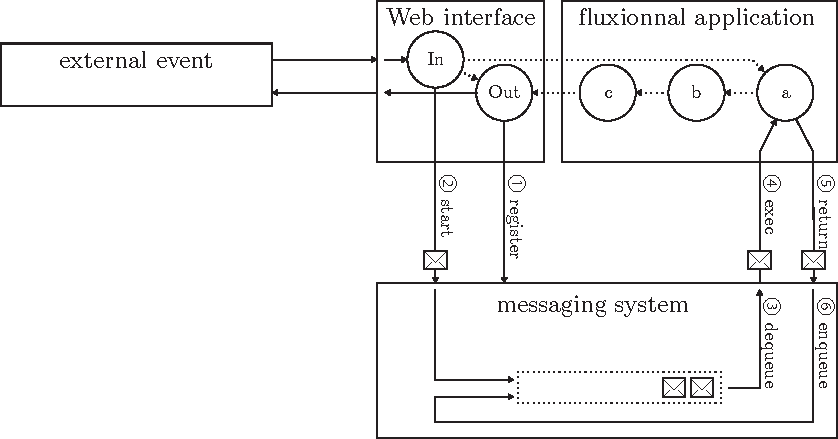
\includegraphics[width=0.5\textwidth]{schema-web.pdf}
	\caption{Schema d'un système fluxionnel avec une interface web}
	\label{fig:schemaweb}
\end{figure}

Le système Web est donc le déclencheur d'une chaîne de traitement de requêtes à chaque nouvelle requête d'un utilisateur un appel à la fonction \lstinline|start('/', <param>)| est réalisé dans le système de messagerie.
Au démarrage du système Web, deux fluxions de bordure sont lancées.
La fluxion de bordure 'in' n'est pas enregistré dans le système de messagerie.
Elle prend les paramètres de la requête Web, place l'identifiant de la connexion client dans le contexte de la demi-fluxion de sortie, puis lance le traitement de la requête en invoquant la fonction `start` du système de messagerie.

\subsection{Exemple de fluxion}

\TODO{}







\section{Performance evaluation}

We use the web service example described in the previous section, Figure \ref{fig:fluxions}, to compare the fluxionnal execution model and the basic Javascript implementation, listing \ref{lst:classique}.
For this evaluation we developed several fluxionnal execution models using different instructions for chaining fluxions.
Thus, through multiple implementation, we can compare the efficiency of the model itself, not of one implementation.

\subsection{About the message queue}

To implement the message queue in Javascript, we used already existing mechanisms as Javascript interpreters are oftnely packaged with an event loop.
We distinguishe three different ways to queue and dequeue messages. These three implementations come the nature of the \texttt{node.js} event loop, and how Javascripts event are processed.

As shown in Figure \ref{fig:eventloop} detailing the different layers of the event loop, the \texttt{node.js} event loop queues messages.
These messages queues stacks of function, which queues functions.
One can queue a message using \texttt{setTimeout}.
Inside a message, one can queue a stack using the \texttt{node.js} instruction \texttt{process.nextTick}.
Inside a stack, one can stack a function by calling directly this function.

Network messages come from I/O operations, thus, they are queued as a new message in the event loop.
So to get network messages, the current message have to end, in order to get the next one, might it come from the network.
However, it's well known that queueing messages in the event loop is far from efficient.

\begin{figure}[h!]
  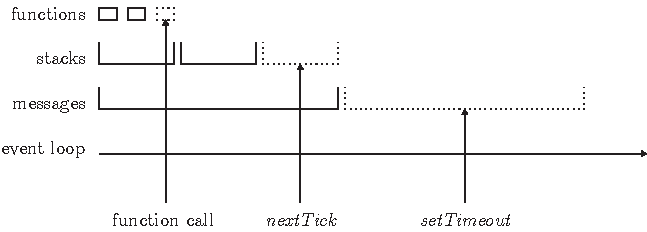
\includegraphics[width=\linewidth]{eventloop.pdf}
  \caption{Javascript event loop details}
  \label{fig:eventloop}
\end{figure}

\subsection{Three different implementations}

We tested our model with three different implementations.

\begin{itemize}
	\item[\textbf{Chain}]
		This implementation chains fluxions one after another by a direct function call.
		The whole fluxion chain is contain inside a same stack on Figure \ref{fig:eventloop}.
		It set the fluxions chain length maximum to the macimum function call stack size, and it's impossible to interleave messages from network in the middle of a fluxion chain.

	\item[\textbf{NextTick}]
		This implementation uses the instruction \texttt{process.nextTick} to chain fluxions execution.
		This instruction add a function call at the end of the current execution.
		Two local fluxion processing chain could run concurrently, but it's only possible to probe network messages every \textit{n} fluxions execution.
		By default \textit{n} is set to 1000.

	\item[\textbf{SetTimeout}]
		This implementation uses the instruction \texttt{setTimeout}.
		It probes network messages after every fluxion execution, thus networks messages can be interleaved between each local messages.
\end{itemize}

With these differents implementations, we want to highlight the advantages and drawbacks of the fluxionnal execution model.

% \begin{figure}
% \begin{tikzpicture}
\begin{axis}[ybar, ylabel={Average response time}, nodes near coords, nodes near coords align={vertical}, xtick=data, x tick label style={rotate=45,anchor=east}, symbolic x coords={chain, basic, nextTick, setTimeout}]
\addplot[color=black]
coordinates {(chain,30542.77957)(basic,55281.24429)(nextTick,80505.31194)(setTimeout,156418.66783)};
\end{axis}
\end{tikzpicture}

% \caption{Average response time for each implementation - 100 parallel clients, sequentillay connecting 1000 times}
% \label{fig:reponsetime}
% \end{figure}

% \begin{figure}
% \begin{tikzpicture}
\begin{semilogxaxis}[xmin=0,xmax=1000000, ylabel=Number of client, xlabel=Response time (ms)]
\addplot[color=blue, mark=x] coordinates {(6900,1)(9700,1)(10800,1)(11500,1)(11900,2)(12100,1)(12300,3)(12400,4)(12500,15)(12600,11)(12700,12)(12800,43)(12900,39)(13000,33)(13100,37)(13200,62)(13300,49)(13400,72)(13500,99)(13600,90)(13700,104)(13800,122)(13900,136)(14000,119)(14100,104)(14200,175)(14300,110)(14400,119)(14500,185)(14600,173)(14700,159)(14800,192)(14900,208)(15000,197)(15100,259)(15200,238)(15300,225)(15400,298)(15500,316)(15600,255)(15700,275)(15800,284)(15900,314)(16000,301)(16100,335)(16200,338)(16300,385)(16400,364)(16500,365)(16600,361)(16700,369)(16800,371)(16900,467)(17000,469)(17100,478)(17200,487)(17300,435)(17400,497)(17500,557)(17600,555)(17700,614)(17800,635)(17900,528)(18000,596)(18100,598)(18200,496)(18300,603)(18400,595)(18500,536)(18600,501)(18700,495)(18800,514)(18900,478)(19000,510)(19100,464)(19200,470)(19300,518)(19400,496)(19500,597)(19600,530)(19700,556)(19800,604)(19900,615)(20000,586)(20100,597)(20200,616)(20300,594)(20400,579)(20500,594)(20600,625)(20700,572)(20800,536)(20900,561)(21000,534)(21100,611)(21200,595)(21300,540)(21400,546)(21500,546)(21600,500)(21700,523)(21800,540)(21900,513)(22000,514)(22100,510)(22200,458)(22300,516)(22400,490)(22500,458)(22600,515)(22700,451)(22800,432)(22900,456)(23000,425)(23100,417)(23200,393)(23300,437)(23400,403)(23500,395)(23600,417)(23700,390)(23800,401)(23900,448)(24000,382)(24100,367)(24200,389)(24300,388)(24400,438)(24500,431)(24600,425)(24700,441)(24800,435)(24900,412)(25000,396)(25100,368)(25200,366)(25300,415)(25400,386)(25500,358)(25600,367)(25700,328)(25800,341)(25900,306)(26000,315)(26100,332)(26200,306)(26300,276)(26400,267)(26500,298)(26600,279)(26700,281)(26800,261)(26900,291)(27000,261)(27100,265)(27200,264)(27300,278)(27400,272)(27500,296)(27600,252)(27700,282)(27800,304)(27900,314)(28000,220)(28100,257)(28200,242)(28300,227)(28400,254)(28500,255)(28600,244)(28700,215)(28800,228)(28900,224)(29000,220)(29100,239)(29200,257)(29300,287)(29400,279)(29500,229)(29600,238)(29700,248)(29800,242)(29900,262)(30000,282)(30100,227)(30200,234)(30300,266)(30400,229)(30500,267)(30600,285)(30700,248)(30800,270)(30900,253)(31000,250)(31100,297)(31200,290)(31300,260)(31400,256)(31500,229)(31600,226)(31700,247)(31800,225)(31900,252)(32000,218)(32100,239)(32200,205)(32300,243)(32400,203)(32500,175)(32600,176)(32700,172)(32800,192)(32900,193)(33000,170)(33100,168)(33200,181)(33300,209)(33400,192)(33500,184)(33600,183)(33700,206)(33800,203)(33900,203)(34000,215)(34100,173)(34200,208)(34300,191)(34400,202)(34500,189)(34600,146)(34700,166)(34800,192)(34900,190)(35000,172)(35100,158)(35200,223)(35300,162)(35400,187)(35500,182)(35600,179)(35700,163)(35800,169)(35900,153)(36000,161)(36100,118)(36200,127)(36300,156)(36400,155)(36500,133)(36600,142)(36700,169)(36800,151)(36900,179)(37000,156)(37100,146)(37200,142)(37300,146)(37400,182)(37500,175)(37600,199)(37700,179)(37800,155)(37900,165)(38000,156)(38100,182)(38200,135)(38300,156)(38400,144)(38500,157)(38600,152)(38700,140)(38800,158)(38900,146)(39000,119)(39100,134)(39200,118)(39300,112)(39400,139)(39500,124)(39600,137)(39700,132)(39800,116)(39900,153)(40000,132)(40100,146)(40200,137)(40300,132)(40400,127)(40500,133)(40600,133)(40700,131)(40800,112)(40900,136)(41000,119)(41100,124)(41200,145)(41300,117)(41400,127)(41500,121)(41600,150)(41700,101)(41800,142)(41900,110)(42000,107)(42100,129)(42200,108)(42300,133)(42400,117)(42500,128)(42600,123)(42700,115)(42800,126)(42900,126)(43000,126)(43100,134)(43200,130)(43300,162)(43400,105)(43500,112)(43600,139)(43700,163)(43800,99)(43900,99)(44000,120)(44100,110)(44200,104)(44300,92)(44400,108)(44500,117)(44600,112)(44700,105)(44800,80)(44900,114)(45000,111)(45100,98)(45200,110)(45300,102)(45400,115)(45500,83)(45600,94)(45700,95)(45800,98)(45900,114)(46000,90)(46100,93)(46200,50)(46300,75)(46400,75)(46500,64)(46600,63)(46700,70)(46800,70)(46900,85)(47000,74)(47100,82)(47200,84)(47300,58)(47400,65)(47500,67)(47600,68)(47700,60)(47800,71)(47900,68)(48000,66)(48100,55)(48200,65)(48300,59)(48400,66)(48500,57)(48600,58)(48700,57)(48800,55)(48900,52)(49000,60)(49100,65)(49200,64)(49300,58)(49400,79)(49500,59)(49600,49)(49700,61)(49800,51)(49900,42)(50000,59)(50100,69)(50200,59)(50300,54)(50400,59)(50500,60)(50600,61)(50700,53)(50800,70)(50900,71)(51000,59)(51100,61)(51200,57)(51300,59)(51400,48)(51500,59)(51600,56)(51700,58)(51800,44)(51900,51)(52000,56)(52100,49)(52200,47)(52300,57)(52400,66)(52500,35)(52600,44)(52700,48)(52800,48)(52900,38)(53000,57)(53100,50)(53200,51)(53300,50)(53400,50)(53500,41)(53600,45)(53700,50)(53800,51)(53900,31)(54000,35)(54100,44)(54200,36)(54300,35)(54400,42)(54500,35)(54600,48)(54700,37)(54800,23)(54900,29)(55000,42)(55100,36)(55200,52)(55300,32)(55400,48)(55500,55)(55600,48)(55700,48)(55800,33)(55900,33)(56000,50)(56100,54)(56200,37)(56300,49)(56400,42)(56500,51)(56600,39)(56700,42)(56800,40)(56900,42)(57000,32)(57100,39)(57200,59)(57300,50)(57400,51)(57500,42)(57600,32)(57700,49)(57800,34)(57900,41)(58000,39)(58100,36)(58200,34)(58300,48)(58400,33)(58500,35)(58600,38)(58700,34)(58800,33)(58900,38)(59000,33)(59100,32)(59200,33)(59300,30)(59400,30)(59500,40)(59600,52)(59700,42)(59800,38)(59900,34)(60000,29)(60100,40)(60200,28)(60300,31)(60400,29)(60500,35)(60600,38)(60700,24)(60800,23)(60900,34)(61000,32)(61100,28)(61200,19)(61300,20)(61400,25)(61500,28)(61600,12)(61700,25)(61800,24)(61900,9)(62000,17)(62100,16)(62200,18)(62300,17)(62400,22)(62500,19)(62600,17)(62700,16)(62800,14)(62900,17)(63000,11)(63100,14)(63200,16)(63300,15)(63400,17)(63500,10)(63600,9)(63700,10)(63800,9)(63900,13)(64000,13)(64100,10)(64200,23)(64300,13)(64400,10)(64500,8)(64600,13)(64700,16)(64800,14)(64900,7)(65000,12)(65100,19)(65200,18)(65300,13)(65400,16)(65500,13)(65600,15)(65700,14)(65800,12)(65900,15)(66000,12)(66100,10)(66200,19)(66300,15)(66400,14)(66500,10)(66600,16)(66700,12)(66800,11)(66900,12)(67000,13)(67100,16)(67200,8)(67300,11)(67400,9)(67500,7)(67600,9)(67700,8)(67800,4)(67900,5)(68000,1)(68100,8)(68200,6)(68300,4)(68400,6)(68500,5)(68600,5)(68700,8)(68800,5)(68900,3)(69000,8)(69100,6)(69200,1)(69300,7)(69400,6)(69500,7)(69600,3)(69700,6)(69800,12)(69900,9)(70000,7)(70100,5)(70200,7)(70300,13)(70400,5)(70500,5)(70600,6)(70700,5)(70800,3)(70900,10)(71000,7)(71100,14)(71200,5)(71300,9)(71400,5)(71500,7)(71600,8)(71700,10)(71800,8)(71900,6)(72000,3)(72100,5)(72200,2)(72300,7)(72400,5)(72500,8)(72600,3)(72700,7)(72800,8)(72900,5)(73000,11)(73100,10)(73200,18)(73300,13)(73400,7)(73500,7)(73600,7)(73700,2)(73800,4)(73900,6)(74000,7)(74100,5)(74200,5)(74300,2)(74400,3)(74500,3)(74600,5)(74700,1)(74800,7)(74900,2)(75000,3)(75100,3)(75200,2)(75300,6)(75400,2)(75500,6)(75600,4)(75700,2)(75800,6)(75900,7)(76000,4)(76100,3)(76200,6)(76300,5)(76400,1)(76500,5)(76600,6)(76700,3)(76800,5)(76900,5)(77000,8)(77100,5)(77200,5)(77300,3)(77400,4)(77500,8)(77600,3)(77700,2)(77800,5)(77900,6)(78000,14)(78100,4)(78200,7)(78300,14)(78400,16)(78500,17)(78600,10)(78700,18)(78800,10)(78900,12)(79000,13)(79100,7)(79200,14)(79300,13)(79400,16)(79500,17)(79600,12)(79700,26)(79800,18)(79900,8)(80000,14)(80100,14)(80200,10)(80300,12)(80400,15)(80500,16)(80600,11)(80700,13)(80800,8)(80900,12)(81000,7)(81100,9)(81200,6)(81300,9)(81400,16)(81500,9)(81600,9)(81700,3)(81800,10)(81900,7)(82000,11)(82100,9)(82200,8)(82300,13)(82400,11)(82500,9)(82600,7)(82700,8)(82800,10)(82900,8)(83000,3)(83100,8)(83200,6)(83300,3)(83400,5)(83500,8)(83600,6)(83700,11)(83800,8)(83900,6)(84000,4)(84100,7)(84200,7)(84300,8)(84400,5)(84500,1)(84600,3)(84700,7)(84800,2)(84900,5)(85000,9)(85100,3)(85200,7)(85300,5)(85400,9)(85500,6)(85600,9)(85700,6)(85800,6)(85900,10)(86000,5)(86100,10)(86200,7)(86300,5)(86400,7)(86500,11)(86600,11)(86700,5)(86800,13)(86900,7)(87000,11)(87100,3)(87200,6)(87300,6)(87400,6)(87500,10)(87600,5)(87700,5)(87800,5)(87900,5)(88000,6)(88100,6)(88200,4)(88300,2)(88400,6)(88500,7)(88600,6)(88700,3)(88800,5)(88900,3)(89000,7)(89100,4)(89200,2)(89300,4)(89400,8)(89500,7)(89600,2)(89700,3)(89800,9)(89900,7)(90000,5)(90100,8)(90200,11)(90300,3)(90400,10)(90500,3)(90600,4)(90700,10)(90800,5)(90900,7)(91000,9)(91100,6)(91200,7)(91300,9)(91400,3)(91500,4)(91600,4)(91700,4)(91800,4)(91900,4)(92000,2)(92100,2)(92200,5)(92300,3)(92400,4)(92500,3)(92600,2)(92700,2)(92800,2)(92900,2)(93000,2)(93100,7)(93200,11)(93300,3)(93400,6)(93500,7)(93600,8)(93700,10)(93800,6)(93900,8)(94000,8)(94100,10)(94200,5)(94300,4)(94400,11)(94500,13)(94600,8)(94700,8)(94800,9)(94900,6)(95000,9)(95100,6)(95200,4)(95300,5)(95400,5)(95500,3)(95600,1)(95700,1)(95900,1)(96000,1)(96100,3)(96200,3)(96300,1)(96500,1)(96600,2)(96700,2)(96900,2)(97100,1)(97700,2)(97800,1)(98000,2)(98200,1)(98300,1)(98400,1)(98700,2)(98800,1)(99100,1)(99200,3)(99400,2)(99500,2)(99900,2)(100000,1)(100200,2)(100400,2)(100500,1)(100800,1)(100900,3)(101000,1)(101100,1)(101200,2)(101500,3)(101600,1)(101700,1)(101900,2)(102400,1)(103100,1)(103500,1)(103800,1)(104300,1)(104500,1)(105200,1)(105300,2)(105500,1)(105600,1)(106400,1)(106500,2)(106600,3)(106800,1)(106900,1)(107200,1)(107400,2)(107500,4)(107600,1)(107700,5)(107800,2)(107900,3)(108000,2)(108100,2)(108200,1)(108300,1)(108400,2)(108500,3)(108600,2)(108700,2)(108800,1)(108900,4)(109000,2)(109200,1)(109300,1)(109700,1)(110000,2)(110100,4)(110300,1)(110500,1)(110600,2)(110700,2)(110800,1)(111200,1)(111300,1)(111400,1)(111500,1)(111600,1)(111700,3)(111900,1)(112700,2)(114500,2)(114600,1)(115400,1)(132400,1)(132500,1)(133000,2)(133200,1)(136700,1)(137000,1)(138100,1)(138300,1)(138400,1)(138500,2)(138600,2)(138700,3)(138800,7)(139000,3)(139100,1)(139200,1)(139400,1)(139500,3)(139600,5)(139700,1)(139800,1)(140000,1)(140300,1)(140500,2)(140600,4)(140800,4)(140900,2)(141000,5)(141200,1)(141300,2)(141400,1)(141500,1)(141600,3)(141700,1)(141800,1)(141900,1)(142100,1)(142400,1)(142500,1)(142900,1)(143000,1)(143100,1)(143200,3)(143500,1)(143600,2)(143700,1)(143900,1)(144000,1)(144200,2)(144300,1)(144400,1)(144500,1)(144600,2)(144700,1)(144800,2)(144900,1)(145000,2)(145100,6)(145200,2)(145300,13)(145400,5)(145500,5)(145600,3)(145700,3)(145800,4)(145900,3)(146000,7)(146100,5)(146200,3)(146300,2)(146400,3)(146500,1)(146600,1)(146700,3)(146900,2)(147000,3)(147100,1)(147300,1)(147400,1)(147600,3)(147700,3)(147800,3)(147900,2)(148000,3)(148100,2)(148200,1)(148400,3)(148500,1)(148600,1)(148700,3)(153200,3)(153300,2)(154000,1)(154200,1)(154700,1)(197500,2)(197600,1)(198100,1)(238600,1)(238900,1)(239200,1)(278700,1)(278800,1)(279500,1)(283900,1)(284000,1)(284200,1)(284300,1)(284500,1)(284800,1)(285200,1)(285500,1)(318700,1)(319100,1)(319300,1)(319400,1)(398500,1)(398700,2)(398900,2)(399100,1)(399300,1)(399500,1)(399600,1)(399800,4)(400200,3)(400300,6)(400400,4)(400600,1)(400700,2)(400900,1)(401000,1)(401100,1)(401300,2)(401400,3)(401500,1)(401600,1)(401800,2)(402100,1)(402200,2)(402400,1)(402500,4)(402800,1)(402900,1)(403000,1)(403500,1)(403800,1)(404200,1)(405500,1)(406300,2)(406500,1)(407200,1)(407400,2)(407600,1)(407900,1)(408000,1)(408100,1)(408600,1)(408700,1)(409000,1)(409300,1)(409600,3)(410600,1)(411100,1)(411300,1)(411500,1)(412100,1)(412300,1)(412500,1)(412700,1)(413400,1)(414100,1)(414800,1)(415500,1)(416300,1)(416400,3)(416500,1)(416600,1)(416800,1)(416900,1)(417500,1)(418100,1)(418300,1)(495600,1)(495900,1)(496300,5)(496400,3)(496500,6)(496600,5)(496700,2)(496800,8)(496900,5)(497100,5)(497200,4)(497300,5)(497400,3)(497500,8)(497600,13)(497700,2)(497800,2)(497900,2)(498000,1)(498100,1)(498200,1)(498300,2)(498400,3)(498500,1)};
\addplot[color=red, mark=x] coordinates {(8000,3)(8200,1)(8600,1)(9100,1)(9300,1)(9400,1)(9600,1)(9700,2)(10000,1)(11300,2)(11500,2)(11800,1)(12100,1)(12400,5)(12500,7)(12600,2)(12700,12)(12800,46)(12900,63)(13000,54)(13100,80)(13200,104)(13300,113)(13400,162)(13500,177)(13600,216)(13700,242)(13800,268)(13900,317)(14000,329)(14100,401)(14200,450)(14300,430)(14400,460)(14500,504)(14600,522)(14700,527)(14800,523)(14900,501)(15000,568)(15100,598)(15200,513)(15300,568)(15400,558)(15500,524)(15600,555)(15700,519)(15800,594)(15900,468)(16000,523)(16100,511)(16200,574)(16300,567)(16400,653)(16500,597)(16600,704)(16700,723)(16800,699)(16900,636)(17000,672)(17100,701)(17200,633)(17300,656)(17400,665)(17500,651)(17600,642)(17700,668)(17800,729)(17900,662)(18000,672)(18100,705)(18200,698)(18300,677)(18400,616)(18500,574)(18600,655)(18700,635)(18800,604)(18900,590)(19000,593)(19100,607)(19200,566)(19300,620)(19400,554)(19500,603)(19600,611)(19700,694)(19800,604)(19900,584)(20000,616)(20100,622)(20200,587)(20300,624)(20400,658)(20500,659)(20600,686)(20700,750)(20800,709)(20900,722)(21000,681)(21100,648)(21200,695)(21300,647)(21400,681)(21500,673)(21600,691)(21700,662)(21800,630)(21900,670)(22000,566)(22100,652)(22200,664)(22300,620)(22400,662)(22500,589)(22600,560)(22700,545)(22800,594)(22900,537)(23000,517)(23100,556)(23200,520)(23300,507)(23400,529)(23500,452)(23600,501)(23700,455)(23800,470)(23900,471)(24000,503)(24100,465)(24200,428)(24300,414)(24400,407)(24500,396)(24600,390)(24700,401)(24800,393)(24900,366)(25000,375)(25100,338)(25200,354)(25300,317)(25400,300)(25500,291)(25600,295)(25700,334)(25800,335)(25900,306)(26000,320)(26100,318)(26200,287)(26300,290)(26400,254)(26500,293)(26600,270)(26700,235)(26800,226)(26900,245)(27000,238)(27100,235)(27200,261)(27300,264)(27400,263)(27500,252)(27600,282)(27700,238)(27800,267)(27900,290)(28000,264)(28100,267)(28200,252)(28300,255)(28400,275)(28500,242)(28600,251)(28700,264)(28800,249)(28900,231)(29000,248)(29100,259)(29200,229)(29300,206)(29400,194)(29500,202)(29600,212)(29700,212)(29800,180)(29900,187)(30000,185)(30100,188)(30200,170)(30300,156)(30400,211)(30500,174)(30600,187)(30700,182)(30800,186)(30900,181)(31000,196)(31100,172)(31200,164)(31300,184)(31400,196)(31500,191)(31600,203)(31700,154)(31800,172)(31900,186)(32000,195)(32100,188)(32200,177)(32300,193)(32400,161)(32500,151)(32600,172)(32700,171)(32800,198)(32900,163)(33000,173)(33100,166)(33200,184)(33300,143)(33400,141)(33500,162)(33600,135)(33700,163)(33800,150)(33900,144)(34000,101)(34100,161)(34200,131)(34300,152)(34400,132)(34500,120)(34600,102)(34700,110)(34800,137)(34900,116)(35000,118)(35100,92)(35200,122)(35300,86)(35400,84)(35500,81)(35600,97)(35700,114)(35800,100)(35900,104)(36000,105)(36100,94)(36200,110)(36300,110)(36400,121)(36500,121)(36600,100)(36700,115)(36800,119)(36900,95)(37000,106)(37100,115)(37200,112)(37300,112)(37400,100)(37500,78)(37600,90)(37700,86)(37800,84)(37900,113)(38000,92)(38100,78)(38200,82)(38300,53)(38400,67)(38500,64)(38600,76)(38700,82)(38800,77)(38900,83)(39000,69)(39100,58)(39200,50)(39300,53)(39400,75)(39500,70)(39600,65)(39700,77)(39800,83)(39900,67)(40000,62)(40100,77)(40200,72)(40300,86)(40400,86)(40500,84)(40600,76)(40700,67)(40800,71)(40900,78)(41000,81)(41100,74)(41200,63)(41300,82)(41400,61)(41500,78)(41600,69)(41700,86)(41800,63)(41900,38)(42000,64)(42100,79)(42200,39)(42300,64)(42400,72)(42500,77)(42600,68)(42700,57)(42800,82)(42900,52)(43000,56)(43100,66)(43200,59)(43300,51)(43400,57)(43500,43)(43600,49)(43700,45)(43800,70)(43900,43)(44000,43)(44100,54)(44200,55)(44300,52)(44400,41)(44500,29)(44600,37)(44700,74)(44800,43)(44900,40)(45000,46)(45100,43)(45200,40)(45300,51)(45400,40)(45500,50)(45600,48)(45700,41)(45800,58)(45900,40)(46000,46)(46100,34)(46200,43)(46300,50)(46400,36)(46500,55)(46600,40)(46700,40)(46800,40)(46900,36)(47000,36)(47100,23)(47200,36)(47300,40)(47400,48)(47500,36)(47600,28)(47700,40)(47800,40)(47900,38)(48000,47)(48100,26)(48200,31)(48300,41)(48400,37)(48500,42)(48600,35)(48700,45)(48800,38)(48900,31)(49000,36)(49100,47)(49200,30)(49300,37)(49400,32)(49500,36)(49600,27)(49700,20)(49800,22)(49900,23)(50000,26)(50100,28)(50200,28)(50300,26)(50400,34)(50500,47)(50600,33)(50700,27)(50800,32)(50900,27)(51000,26)(51100,17)(51200,26)(51300,29)(51400,23)(51500,25)(51600,29)(51700,29)(51800,28)(51900,27)(52000,27)(52100,13)(52200,19)(52300,26)(52400,19)(52500,21)(52600,42)(52700,33)(52800,27)(52900,29)(53000,29)(53100,33)(53200,29)(53300,36)(53400,30)(53500,35)(53600,37)(53700,30)(53800,33)(53900,23)(54000,23)(54100,28)(54200,26)(54300,28)(54400,42)(54500,31)(54600,59)(54700,25)(54800,22)(54900,31)(55000,14)(55100,13)(55200,9)(55300,22)(55400,29)(55500,26)(55600,11)(55700,15)(55800,31)(55900,22)(56000,19)(56100,17)(56200,17)(56300,30)(56400,15)(56500,12)(56600,19)(56700,22)(56800,26)(56900,21)(57000,25)(57100,20)(57200,15)(57300,19)(57400,19)(57500,17)(57600,17)(57700,21)(57800,19)(57900,17)(58000,10)(58100,12)(58200,16)(58300,21)(58400,13)(58500,7)(58600,10)(58700,9)(58800,15)(58900,14)(59000,6)(59100,6)(59200,10)(59300,12)(59400,10)(59500,11)(59600,9)(59700,7)(59800,6)(59900,12)(60000,12)(60100,11)(60200,8)(60300,10)(60400,16)(60500,9)(60600,12)(60700,11)(60800,8)(60900,11)(61000,7)(61100,7)(61200,8)(61300,8)(61400,10)(61500,22)(61600,15)(61700,9)(61800,7)(61900,13)(62000,10)(62100,8)(62200,3)(62300,6)(62400,3)(62500,10)(62600,6)(62700,6)(62800,5)(62900,4)(63000,2)(63100,3)(63200,4)(63300,1)(63400,8)(63500,3)(63600,4)(63700,2)(63800,5)(63900,9)(64000,4)(64100,3)(64200,7)(64300,7)(64400,5)(64500,6)(64600,5)(64700,5)(64800,5)(64900,1)(65000,2)(65100,6)(65200,3)(65300,10)(65400,9)(65500,5)(65600,10)(65700,4)(65800,2)(65900,5)(66000,1)(66100,2)(66200,4)(66300,5)(66400,4)(66500,2)(66600,3)(66700,6)(66800,5)(66900,4)(67000,3)(67100,4)(67200,4)(67300,6)(67400,3)(67500,3)(67600,2)(67800,2)(67900,2)(68000,3)(68100,3)(68200,1)(68400,1)(68500,4)(68600,7)(68800,4)(68900,3)(69000,3)(69100,1)(69200,5)(69300,4)(69400,2)(69500,3)(69600,2)(69800,3)(69900,3)(70200,3)(70300,3)(70400,2)(70500,3)(70600,6)(70700,5)(70800,2)(70900,5)(71000,5)(71100,3)(71200,1)(71300,6)(71400,2)(71500,3)(71600,4)(71700,6)(71800,7)(71900,5)(72000,7)(72100,2)(72200,5)(72300,3)(72400,9)(72500,1)(72600,5)(72700,7)(72800,8)(72900,3)(73000,3)(73100,5)(73200,9)(73300,7)(73400,1)(73500,2)(73600,2)(73700,3)(73800,3)(73900,5)(74000,1)(74100,9)(74200,5)(74300,3)(74400,3)(74500,2)(74600,1)(74700,1)(74800,2)(75000,6)(75100,3)(75200,1)(75300,4)(75400,2)(75500,4)(75600,5)(75700,1)(75800,2)(75900,2)(76000,5)(76200,1)(76400,5)(76500,3)(76600,2)(76700,2)(76800,2)(77000,3)(77100,2)(77200,1)(77400,1)(77500,3)(77600,2)(77700,1)(77800,1)(77900,2)(78000,3)(78100,2)(78200,1)(78300,1)(78400,1)(78500,1)(78700,2)(78800,6)(78900,2)(79000,2)(79100,5)(79200,5)(79300,5)(79400,1)(79500,6)(79600,3)(79700,2)(79800,3)(79900,3)(80100,6)(80300,1)(80500,1)(80700,1)(80800,2)(80900,1)(81000,2)(81200,3)(81300,1)(81400,2)(81500,1)(81600,1)(81700,1)(81900,2)(82000,2)(82200,1)(82300,1)(82500,1)(82600,1)(82800,1)(83000,1)(83100,1)(83200,1)(83300,1)(83400,1)(83600,2)(83900,2)(84300,3)(84700,2)(85000,2)(85400,2)(85500,3)(86300,1)(87100,1)(87600,2)(87900,1)(88100,1)(88200,1)(88500,1)(88900,1)(89300,2)(89700,1)(90000,1)(90100,2)(90200,2)(90600,2)(91000,2)(91200,2)(91300,1)(91400,2)(91600,4)(91700,1)(91800,1)(91900,1)(92000,2)(92200,1)(92400,1)(92600,1)(92700,1)(92800,1)(92900,1)(93000,1)(93200,1)(93300,1)(93400,2)(93500,1)(93600,1)(93700,1)(93800,1)(94100,1)(94200,1)(94300,1)(94500,1)(94600,2)(94700,1)(94800,1)(95300,2)};
\addplot[color=green, mark=x] coordinates {(7100,1)(7300,1)(7600,1)(7700,1)(7800,1)(10300,1)(11300,1)(11500,1)(11600,3)(11700,17)(11800,64)(11900,73)(12000,73)(12100,79)(12200,116)(12300,102)(12400,82)(12500,82)(12600,89)(12700,142)(12800,186)(12900,175)(13000,277)(13100,298)(13200,318)(13300,425)(13400,484)(13500,364)(13600,365)(13700,414)(13800,488)(13900,509)(14000,532)(14100,503)(14200,516)(14300,515)(14400,595)(14500,655)(14600,595)(14700,717)(14800,662)(14900,693)(15000,678)(15100,702)(15200,704)(15300,698)(15400,672)(15500,653)(15600,673)(15700,593)(15800,564)(15900,564)(16000,489)(16100,521)(16200,489)(16300,451)(16400,456)(16500,413)(16600,458)(16700,473)(16800,441)(16900,435)(17000,479)(17100,485)(17200,476)(17300,487)(17400,544)(17500,566)(17600,558)(17700,599)(17800,548)(17900,511)(18000,547)(18100,606)(18200,583)(18300,589)(18400,587)(18500,635)(18600,602)(18700,616)(18800,680)(18900,621)(19000,632)(19100,644)(19200,700)(19300,698)(19400,742)(19500,667)(19600,644)(19700,629)(19800,668)(19900,642)(20000,741)(20100,708)(20200,641)(20300,621)(20400,724)(20500,688)(20600,628)(20700,643)(20800,633)(20900,557)(21000,625)(21100,590)(21200,556)(21300,537)(21400,521)(21500,523)(21600,523)(21700,477)(21800,531)(21900,496)(22000,504)(22100,449)(22200,499)(22300,479)(22400,494)(22500,509)(22600,502)(22700,494)(22800,487)(22900,488)(23000,530)(23100,515)(23200,454)(23300,490)(23400,461)(23500,441)(23600,453)(23700,415)(23800,423)(23900,428)(24000,388)(24100,384)(24200,323)(24300,387)(24400,410)(24500,378)(24600,395)(24700,383)(24800,348)(24900,361)(25000,394)(25100,393)(25200,328)(25300,365)(25400,379)(25500,362)(25600,345)(25700,341)(25800,322)(25900,321)(26000,329)(26100,331)(26200,303)(26300,301)(26400,300)(26500,303)(26600,313)(26700,249)(26800,273)(26900,241)(27000,276)(27100,284)(27200,235)(27300,242)(27400,222)(27500,230)(27600,208)(27700,185)(27800,212)(27900,193)(28000,180)(28100,202)(28200,228)(28300,253)(28400,207)(28500,203)(28600,196)(28700,163)(28800,194)(28900,210)(29000,232)(29100,228)(29200,236)(29300,239)(29400,210)(29500,209)(29600,172)(29700,172)(29800,182)(29900,169)(30000,181)(30100,160)(30200,147)(30300,181)(30400,131)(30500,156)(30600,146)(30700,165)(30800,155)(30900,176)(31000,188)(31100,142)(31200,168)(31300,166)(31400,176)(31500,171)(31600,194)(31700,192)(31800,178)(31900,188)(32000,159)(32100,190)(32200,183)(32300,171)(32400,168)(32500,157)(32600,145)(32700,153)(32800,148)(32900,140)(33000,121)(33100,151)(33200,134)(33300,115)(33400,128)(33500,118)(33600,96)(33700,105)(33800,107)(33900,94)(34000,121)(34100,85)(34200,87)(34300,82)(34400,86)(34500,88)(34600,122)(34700,98)(34800,84)(34900,79)(35000,87)(35100,72)(35200,93)(35300,102)(35400,116)(35500,102)(35600,94)(35700,97)(35800,86)(35900,81)(36000,105)(36100,92)(36200,91)(36300,134)(36400,112)(36500,118)(36600,127)(36700,129)(36800,119)(36900,113)(37000,80)(37100,89)(37200,74)(37300,81)(37400,87)(37500,85)(37600,82)(37700,76)(37800,83)(37900,85)(38000,94)(38100,103)(38200,87)(38300,96)(38400,77)(38500,79)(38600,104)(38700,94)(38800,89)(38900,102)(39000,80)(39100,124)(39200,83)(39300,88)(39400,95)(39500,101)(39600,87)(39700,84)(39800,99)(39900,97)(40000,105)(40100,86)(40200,93)(40300,102)(40400,81)(40500,86)(40600,84)(40700,91)(40800,72)(40900,75)(41000,73)(41100,88)(41200,82)(41300,77)(41400,82)(41500,75)(41600,68)(41700,101)(41800,78)(41900,80)(42000,72)(42100,96)(42200,77)(42300,79)(42400,89)(42500,92)(42600,84)(42700,78)(42800,86)(42900,62)(43000,59)(43100,67)(43200,48)(43300,58)(43400,56)(43500,63)(43600,45)(43700,70)(43800,57)(43900,57)(44000,64)(44100,33)(44200,59)(44300,60)(44400,46)(44500,47)(44600,45)(44700,44)(44800,46)(44900,37)(45000,42)(45100,40)(45200,41)(45300,43)(45400,50)(45500,39)(45600,48)(45700,39)(45800,51)(45900,48)(46000,52)(46100,47)(46200,47)(46300,47)(46400,55)(46500,49)(46600,38)(46700,50)(46800,47)(46900,47)(47000,37)(47100,41)(47200,26)(47300,46)(47400,35)(47500,52)(47600,57)(47700,40)(47800,28)(47900,31)(48000,21)(48100,18)(48200,43)(48300,30)(48400,25)(48500,43)(48600,34)(48700,25)(48800,27)(48900,18)(49000,30)(49100,25)(49200,39)(49300,30)(49400,43)(49500,35)(49600,21)(49700,31)(49800,30)(49900,23)(50000,16)(50100,27)(50200,32)(50300,25)(50400,43)(50500,33)(50600,38)(50700,42)(50800,30)(50900,41)(51000,58)(51100,40)(51200,43)(51300,34)(51400,37)(51500,36)(51600,41)(51700,36)(51800,24)(51900,34)(52000,33)(52100,27)(52200,32)(52300,44)(52400,27)(52500,33)(52600,30)(52700,27)(52800,16)(52900,15)(53000,32)(53100,19)(53200,11)(53300,15)(53400,20)(53500,17)(53600,19)(53700,16)(53800,12)(53900,16)(54000,20)(54100,11)(54200,9)(54300,16)(54400,20)(54500,11)(54600,14)(54700,18)(54800,25)(54900,12)(55000,19)(55100,13)(55200,10)(55300,15)(55400,19)(55500,22)(55600,19)(55700,16)(55800,14)(55900,11)(56000,12)(56100,8)(56200,18)(56300,12)(56400,19)(56500,15)(56600,17)(56700,17)(56800,10)(56900,21)(57000,18)(57100,9)(57200,5)(57300,10)(57400,14)(57500,13)(57600,13)(57700,15)(57800,22)(57900,12)(58000,14)(58100,11)(58200,11)(58300,11)(58400,24)(58500,33)(58600,18)(58700,16)(58800,15)(58900,16)(59000,15)(59100,14)(59200,20)(59300,30)(59400,22)(59500,11)(59600,14)(59700,14)(59800,16)(59900,23)(60000,12)(60100,13)(60200,10)(60300,13)(60400,9)(60500,17)(60600,20)(60700,22)(60800,20)(60900,16)(61000,14)(61100,10)(61200,24)(61300,13)(61400,17)(61500,13)(61600,18)(61700,19)(61800,21)(61900,19)(62000,18)(62100,9)(62200,14)(62300,17)(62400,14)(62500,13)(62600,10)(62700,10)(62800,10)(62900,11)(63000,15)(63100,14)(63200,9)(63300,11)(63400,8)(63500,10)(63600,14)(63700,15)(63800,11)(63900,7)(64000,9)(64100,8)(64200,8)(64300,9)(64400,8)(64500,10)(64600,10)(64700,19)(64800,9)(64900,13)(65000,11)(65100,10)(65200,9)(65300,11)(65400,12)(65500,8)(65600,9)(65700,16)(65800,20)(65900,13)(66000,9)(66100,8)(66200,10)(66300,9)(66400,9)(66500,5)(66600,10)(66700,13)(66800,6)(66900,5)(67000,8)(67100,8)(67200,7)(67300,7)(67400,5)(67500,10)(67600,3)(67700,6)(67800,10)(67900,8)(68000,8)(68100,10)(68200,6)(68300,10)(68400,10)(68500,5)(68600,4)(68700,5)(68800,8)(68900,7)(69000,12)(69100,11)(69200,7)(69300,10)(69400,8)(69500,11)(69600,7)(69700,4)(69800,5)(69900,11)(70000,10)(70100,5)(70200,6)(70300,3)(70400,3)(70500,4)(70600,2)(70700,3)(70800,3)(70900,4)(71000,6)(71100,4)(71200,3)(71300,5)(71400,6)(71500,7)(71600,7)(71700,6)(71900,1)(72000,5)(72100,2)(72200,6)(72300,10)(72400,3)(72500,4)(72600,2)(72700,3)(72800,5)(73000,1)(73100,3)(73200,4)(73300,8)(73400,6)(73500,3)(73600,2)(73700,5)(73800,2)(73900,2)(74000,3)(74100,7)(74200,5)(74300,2)(74400,3)(74500,4)(74600,2)(74700,1)(74800,4)(74900,5)(75000,3)(75100,8)(75200,5)(75300,6)(75400,8)(75500,1)(75600,2)(75700,6)(75800,3)(75900,5)(76000,4)(76100,2)(76200,2)(76300,5)(76400,2)(76500,5)(76600,3)(76700,3)(76800,7)(76900,8)(77000,1)(77100,3)(77200,10)(77300,2)(77400,3)(77500,3)(77600,5)(77700,8)(77800,6)(77900,2)(78000,6)(78100,5)(78200,7)(78300,5)(78400,7)(78500,5)(78600,3)(78700,4)(78800,4)(78900,5)(79000,4)(79100,2)(79200,2)(79300,3)(79400,3)(79500,6)(79600,10)(79700,12)(79800,9)(79900,6)(80000,4)(80100,4)(80200,3)(80300,8)(80400,8)(80500,6)(80600,9)(80700,5)(80800,11)(80900,2)(81000,4)(81100,8)(81200,7)(81300,9)(81400,5)(81500,6)(81600,5)(81700,8)(81800,6)(81900,8)(82000,6)(82100,4)(82200,9)(82300,7)(82400,6)(82500,6)(82600,7)(82700,9)(82800,2)(82900,6)(83000,1)(83100,3)(83200,4)(83300,4)(83400,5)(83500,3)(83600,4)(83700,2)(83800,4)(83900,4)(84000,2)(84100,2)(84200,5)(84300,8)(84400,4)(84500,6)(84600,3)(84700,2)(84800,3)(85000,4)(85100,4)(85200,7)(85300,5)(85400,3)(85500,6)(85600,6)(85700,5)(85800,7)(85900,14)(86000,14)(86100,5)(86200,3)(86300,5)(86400,7)(86500,4)(86600,2)(86700,5)(86800,4)(86900,5)(87000,1)(87100,4)(87200,5)(87300,4)(87400,1)(87500,3)(87600,1)(87700,6)(87800,1)(87900,1)(88000,3)(88100,2)(88200,2)(88300,1)(88400,3)(88500,2)(88600,2)(88700,1)(88800,1)(89000,2)(89100,3)(89200,2)(89400,2)(89500,1)(89900,2)(90000,1)(90200,2)(90300,1)(90700,1)(141000,1)(141300,3)(141500,3)(141600,1)(141800,2)(141900,1)(142000,4)(142100,3)(142200,1)(142300,6)(142400,1)(142600,1)(142700,3)(142800,2)(142900,2)(143000,1)(143200,2)(143300,3)(143600,2)(143700,1)(143800,2)(144000,3)(144100,2)(144400,3)(144700,2)(144800,4)(144900,1)(145000,1)(145100,2)(145300,1)(145500,3)(145900,3)(146000,1)(146100,1)(146200,2)(146300,2)(146400,2)(146500,2)(146600,1)(146700,1)(146900,1)(147000,3)(147100,2)(147200,1)(147300,2)(147500,1)(147900,1)(166900,1)(167000,1)(167300,2)(167400,2)(167500,2)(167700,1)(167900,1)(168100,1)(168500,1)(168900,1)(169000,1)(263900,1)(264400,1)(264500,1)(264600,1)(265000,1)(265400,1)(265600,1)(281800,2)(282700,1)(283100,1)(298900,1)(299000,1)(299200,1)(299400,1)(299600,1)(299800,2)(299900,3)(300000,2)(300100,2)(300400,1)(300600,1)(300800,2)(300900,3)(301000,4)(301200,3)(301300,2)(301400,3)(301500,1)(301600,1)(301700,1)(301900,1)(302100,1)(302200,4)(302300,1)(302600,1)(303100,1)(305100,1)(305200,1)(305500,1)(305600,1)(305700,3)(306200,1)(306300,1)(306500,1)(306600,1)(306800,2)(307400,1)(307600,1)(308000,1)(308900,1)(310200,1)(310500,1)(310700,1)(311300,1)(311700,1)(313300,1)(313500,3)(313900,2)(314000,2)(314200,1)(314300,2)(314400,1)(315200,1)(315400,1)(315500,1)};
\addplot[color=yellow, mark=x] coordinates {(20000,1)(21000,1)(22000,1)(22300,1)(22600,1)(23000,1)(23500,1)(24800,1)(25000,1)(27100,1)(27400,1)(27600,1)(29300,1)(29500,1)(31200,1)(32100,1)(32300,1)(34100,1)(34300,1)(35900,1)(36100,1)(37100,1)(38500,1)(38800,1)(39800,1)(41600,1)(44600,1)(45100,1)(45500,1)(45700,1)(47500,1)(48500,1)(49800,1)(51500,1)(51700,2)(51800,1)(51900,3)(52000,7)(52100,1)(52200,1)(52300,8)(52600,1)(52700,8)(52800,4)(52900,10)(53000,11)(53100,8)(53200,7)(53300,7)(53400,4)(53500,3)(53600,5)(53700,12)(53800,8)(53900,8)(54000,16)(54100,14)(54200,24)(54300,39)(54400,5)(54500,7)(54600,4)(54700,3)(54800,2)(54900,3)(55000,8)(55100,16)(55200,9)(55300,4)(55400,21)(55500,17)(55600,19)(55700,9)(55800,8)(55900,9)(56000,8)(56100,13)(56200,8)(56300,7)(56400,6)(56500,14)(56600,9)(56700,6)(56800,10)(56900,14)(57000,10)(57100,8)(57200,17)(57300,7)(57400,7)(57500,12)(57600,7)(57700,8)(57800,18)(57900,14)(58000,18)(58100,16)(58200,16)(58300,3)(58400,15)(58500,10)(58600,11)(58700,15)(58800,7)(58900,8)(59000,8)(59100,16)(59200,21)(59300,19)(59400,24)(59500,15)(59600,20)(59700,16)(59800,27)(59900,31)(60000,39)(60100,24)(60200,30)(60300,17)(60400,25)(60500,26)(60600,15)(60700,25)(60800,26)(60900,31)(61000,23)(61100,27)(61200,32)(61300,20)(61400,17)(61500,30)(61600,36)(61700,33)(61800,30)(61900,35)(62000,25)(62100,24)(62200,25)(62300,29)(62400,41)(62500,51)(62600,39)(62700,66)(62800,49)(62900,43)(63000,41)(63100,59)(63200,59)(63300,63)(63400,48)(63500,42)(63600,52)(63700,54)(63800,72)(63900,54)(64000,66)(64100,79)(64200,81)(64300,106)(64400,106)(64500,100)(64600,76)(64700,78)(64800,103)(64900,110)(65000,91)(65100,100)(65200,110)(65300,84)(65400,95)(65500,123)(65600,117)(65700,146)(65800,176)(65900,159)(66000,160)(66100,167)(66200,182)(66300,203)(66400,146)(66500,182)(66600,151)(66700,168)(66800,167)(66900,180)(67000,221)(67100,195)(67200,215)(67300,170)(67400,201)(67500,174)(67600,183)(67700,190)(67800,187)(67900,188)(68000,260)(68100,266)(68200,267)(68300,276)(68400,281)(68500,277)(68600,275)(68700,251)(68800,269)(68900,310)(69000,319)(69100,285)(69200,310)(69300,311)(69400,304)(69500,336)(69600,337)(69700,385)(69800,381)(69900,387)(70000,431)(70100,368)(70200,414)(70300,410)(70400,387)(70500,426)(70600,399)(70700,385)(70800,455)(70900,431)(71000,429)(71100,483)(71200,495)(71300,475)(71400,459)(71500,471)(71600,484)(71700,517)(71800,498)(71900,532)(72000,496)(72100,592)(72200,577)(72300,647)(72400,544)(72500,556)(72600,518)(72700,541)(72800,584)(72900,593)(73000,628)(73100,639)(73200,641)(73300,762)(73400,696)(73500,662)(73600,663)(73700,705)(73800,701)(73900,667)(74000,761)(74100,838)(74200,744)(74300,773)(74400,876)(74500,842)(74600,942)(74700,856)(74800,862)(74900,955)(75000,865)(75100,838)(75200,944)(75300,872)(75400,847)(75500,842)(75600,932)(75700,835)(75800,928)(75900,931)(76000,891)(76100,867)(76200,1004)(76300,897)(76400,938)(76500,852)(76600,778)(76700,948)(76800,885)(76900,960)(77000,973)(77100,933)(77200,798)(77300,800)(77400,750)(77500,743)(77600,732)(77700,741)(77800,667)(77900,661)(78000,618)(78100,669)(78200,695)(78300,641)(78400,611)(78500,633)(78600,637)(78700,661)(78800,580)(78900,579)(79000,619)(79100,550)(79200,536)(79300,522)(79400,485)(79500,477)(79600,498)(79700,461)(79800,456)(79900,520)(80000,452)(80100,512)(80200,466)(80300,418)(80400,420)(80500,371)(80600,394)(80700,359)(80800,364)(80900,366)(81000,363)(81100,343)(81200,331)(81300,319)(81400,310)(81500,323)(81600,318)(81700,289)(81800,281)(81900,281)(82000,278)(82100,281)(82200,212)(82300,244)(82400,201)(82500,178)(82600,190)(82700,188)(82800,190)(82900,169)(83000,188)(83100,180)(83200,166)(83300,128)(83400,124)(83500,121)(83600,164)(83700,135)(83800,131)(83900,132)(84000,103)(84100,109)(84200,115)(84300,152)(84400,128)(84500,123)(84600,117)(84700,122)(84800,121)(84900,115)(85000,120)(85100,86)(85200,93)(85300,109)(85400,127)(85500,103)(85600,81)(85700,91)(85800,108)(85900,111)(86000,102)(86100,97)(86200,90)(86300,68)(86400,81)(86500,78)(86600,80)(86700,86)(86800,92)(86900,66)(87000,64)(87100,48)(87200,64)(87300,60)(87400,68)(87500,53)(87600,69)(87700,51)(87800,54)(87900,59)(88000,76)(88100,54)(88200,65)(88300,57)(88400,58)(88500,40)(88600,53)(88700,56)(88800,60)(88900,41)(89000,42)(89100,47)(89200,58)(89300,64)(89400,49)(89500,63)(89600,62)(89700,45)(89800,75)(89900,50)(90000,58)(90100,77)(90200,43)(90300,70)(90400,53)(90500,46)(90600,47)(90700,55)(90800,53)(90900,47)(91000,27)(91100,44)(91200,43)(91300,30)(91400,57)(91500,39)(91600,52)(91700,49)(91800,38)(91900,53)(92000,50)(92100,29)(92200,37)(92300,37)(92400,31)(92500,30)(92600,33)(92700,39)(92800,37)(92900,44)(93000,38)(93100,38)(93200,28)(93300,45)(93400,38)(93500,30)(93600,24)(93700,18)(93800,23)(93900,21)(94000,29)(94100,24)(94200,31)(94300,33)(94400,26)(94500,21)(94600,27)(94700,29)(94800,25)(94900,12)(95000,20)(95100,24)(95200,15)(95300,18)(95400,16)(95500,21)(95600,18)(95700,22)(95800,34)(95900,20)(96000,16)(96100,14)(96200,15)(96300,22)(96400,12)(96500,11)(96600,8)(96700,14)(96800,11)(96900,16)(97000,14)(97100,16)(97200,12)(97300,22)(97400,19)(97500,17)(97600,12)(97700,9)(97800,11)(97900,16)(98000,12)(98100,10)(98200,11)(98300,10)(98400,9)(98500,7)(98600,6)(98700,2)(98800,9)(98900,4)(99000,4)(99100,4)(99200,7)(99300,4)(99400,6)(99500,6)(99600,10)(99700,14)(99800,7)(99900,4)(100000,6)(100100,6)(100200,8)(100300,4)(100400,4)(100500,4)(100600,6)(100700,8)(100800,6)(100900,9)(101000,7)(101100,2)(101300,4)(101400,1)(101500,11)(101600,5)(101700,5)(101800,6)(101900,12)(102000,6)(102100,6)(102200,5)(102300,5)(102400,6)(102500,7)(102600,5)(102700,8)(102800,4)(102900,5)(103000,2)(103100,7)(103200,7)(103300,3)(103400,9)(103500,8)(103600,7)(103700,4)(103800,4)(103900,2)(104000,5)(104100,4)(104200,3)(104300,2)(104400,2)(104500,2)(104600,3)(104700,5)(104800,8)(104900,6)(105000,5)(105100,3)(105200,7)(105300,6)(105400,6)(105500,4)(105600,1)(105700,5)(105800,7)(105900,10)(106000,6)(106100,16)(106200,7)(106300,5)(106400,6)(106500,6)(106600,3)(106700,2)(106800,3)(106900,6)(107000,6)(107100,8)(107200,8)(107300,2)(107400,4)(107500,5)(107600,4)(107700,7)(107800,5)(107900,5)(108000,8)(108100,4)(108200,5)(108300,9)(108400,2)(108500,4)(108600,7)(108700,4)(108800,11)(108900,7)(109000,4)(109100,5)(109200,3)(109300,3)(109500,1)(109600,3)(109700,2)(109800,5)(109900,4)(110000,4)(110200,1)(110400,1)(110500,1)(110600,1)(110700,1)(110800,2)(110900,2)(111000,2)(111200,1)(111300,2)(111500,1)(111600,4)(111700,2)(111800,3)(111900,1)(112000,1)(112100,2)(112200,3)(112300,3)(112500,5)(112700,3)(112800,3)(112900,5)(113000,2)(113100,2)(113300,2)(113400,2)(113500,1)(113600,1)(113700,2)(113800,2)(113900,3)(114000,3)(114100,1)(114300,1)(114600,1)(114700,2)(115000,1)(115200,1)(115300,1)(115400,1)(115500,3)(115600,1)(115800,1)(116200,1)(116400,1)(116500,1)(116600,2)(117000,1)(117100,1)(117300,1)(118100,1)(118300,1)(118600,1)(118800,1)(118900,1)(119000,3)(119100,1)(120100,1)(120300,2)(120400,3)(120500,1)(120600,3)(120800,1)(121000,3)(121100,3)(121200,1)(121300,1)(121400,1)(121600,2)(122000,2)(122200,1)(122500,2)(122700,1)(122900,1)(123000,1)(123400,1)(123900,1)(124600,2)(124900,1)(125500,1)(125600,1)(125700,1)(126000,1)(126500,1)(126700,1)(126900,1)(127100,1)(128200,1)(128300,1)};
\legend{chain, basic, nextTick, setTimeout}
\end{semilogxaxis}
\end{tikzpicture}

% \caption{Distribution of response time for each implementation - 100 parallel clients, sequentillay connecting 1000 times}
% \label{fig:distribution}
% \end{figure}

% \begin{figure}
% \begin{tikzpicture}
\begin{semilogxaxis}[xmin=0,xmax=1000000, ylabel=Number of client, xlabel=Response time (ms)]

\addplot[color=black, mark=x] coordinates {(8000,3)(8200,1)(8600,1)(9100,1)(9300,1)(9400,1)(9600,1)(9700,2)(10000,1)(11300,2)(11500,2)(11800,1)(12100,1)(12400,5)(12500,7)(12600,2)(12700,12)(12800,46)(12900,63)(13000,54)(13100,80)(13200,104)(13300,113)(13400,162)(13500,177)(13600,216)(13700,242)(13800,268)(13900,317)(14000,329)(14100,401)(14200,450)(14300,430)(14400,460)(14500,504)(14600,522)(14700,527)(14800,523)(14900,501)(15000,568)(15100,598)(15200,513)(15300,568)(15400,558)(15500,524)(15600,555)(15700,519)(15800,594)(15900,468)(16000,523)(16100,511)(16200,574)(16300,567)(16400,653)(16500,597)(16600,704)(16700,723)(16800,699)(16900,636)(17000,672)(17100,701)(17200,633)(17300,656)(17400,665)(17500,651)(17600,642)(17700,668)(17800,729)(17900,662)(18000,672)(18100,705)(18200,698)(18300,677)(18400,616)(18500,574)(18600,655)(18700,635)(18800,604)(18900,590)(19000,593)(19100,607)(19200,566)(19300,620)(19400,554)(19500,603)(19600,611)(19700,694)(19800,604)(19900,584)(20000,616)(20100,622)(20200,587)(20300,624)(20400,658)(20500,659)(20600,686)(20700,750)(20800,709)(20900,722)(21000,681)(21100,648)(21200,695)(21300,647)(21400,681)(21500,673)(21600,691)(21700,662)(21800,630)(21900,670)(22000,566)(22100,652)(22200,664)(22300,620)(22400,662)(22500,589)(22600,560)(22700,545)(22800,594)(22900,537)(23000,517)(23100,556)(23200,520)(23300,507)(23400,529)(23500,452)(23600,501)(23700,455)(23800,470)(23900,471)(24000,503)(24100,465)(24200,428)(24300,414)(24400,407)(24500,396)(24600,390)(24700,401)(24800,393)(24900,366)(25000,375)(25100,338)(25200,354)(25300,317)(25400,300)(25500,291)(25600,295)(25700,334)(25800,335)(25900,306)(26000,320)(26100,318)(26200,287)(26300,290)(26400,254)(26500,293)(26600,270)(26700,235)(26800,226)(26900,245)(27000,238)(27100,235)(27200,261)(27300,264)(27400,263)(27500,252)(27600,282)(27700,238)(27800,267)(27900,290)(28000,264)(28100,267)(28200,252)(28300,255)(28400,275)(28500,242)(28600,251)(28700,264)(28800,249)(28900,231)(29000,248)(29100,259)(29200,229)(29300,206)(29400,194)(29500,202)(29600,212)(29700,212)(29800,180)(29900,187)(30000,185)(30100,188)(30200,170)(30300,156)(30400,211)(30500,174)(30600,187)(30700,182)(30800,186)(30900,181)(31000,196)(31100,172)(31200,164)(31300,184)(31400,196)(31500,191)(31600,203)(31700,154)(31800,172)(31900,186)(32000,195)(32100,188)(32200,177)(32300,193)(32400,161)(32500,151)(32600,172)(32700,171)(32800,198)(32900,163)(33000,173)(33100,166)(33200,184)(33300,143)(33400,141)(33500,162)(33600,135)(33700,163)(33800,150)(33900,144)(34000,101)(34100,161)(34200,131)(34300,152)(34400,132)(34500,120)(34600,102)(34700,110)(34800,137)(34900,116)(35000,118)(35100,92)(35200,122)(35300,86)(35400,84)(35500,81)(35600,97)(35700,114)(35800,100)(35900,104)(36000,105)(36100,94)(36200,110)(36300,110)(36400,121)(36500,121)(36600,100)(36700,115)(36800,119)(36900,95)(37000,106)(37100,115)(37200,112)(37300,112)(37400,100)(37500,78)(37600,90)(37700,86)(37800,84)(37900,113)(38000,92)(38100,78)(38200,82)(38300,53)(38400,67)(38500,64)(38600,76)(38700,82)(38800,77)(38900,83)(39000,69)(39100,58)(39200,50)(39300,53)(39400,75)(39500,70)(39600,65)(39700,77)(39800,83)(39900,67)(40000,62)(40100,77)(40200,72)(40300,86)(40400,86)(40500,84)(40600,76)(40700,67)(40800,71)(40900,78)(41000,81)(41100,74)(41200,63)(41300,82)(41400,61)(41500,78)(41600,69)(41700,86)(41800,63)(41900,38)(42000,64)(42100,79)(42200,39)(42300,64)(42400,72)(42500,77)(42600,68)(42700,57)(42800,82)(42900,52)(43000,56)(43100,66)(43200,59)(43300,51)(43400,57)(43500,43)(43600,49)(43700,45)(43800,70)(43900,43)(44000,43)(44100,54)(44200,55)(44300,52)(44400,41)(44500,29)(44600,37)(44700,74)(44800,43)(44900,40)(45000,46)(45100,43)(45200,40)(45300,51)(45400,40)(45500,50)(45600,48)(45700,41)(45800,58)(45900,40)(46000,46)(46100,34)(46200,43)(46300,50)(46400,36)(46500,55)(46600,40)(46700,40)(46800,40)(46900,36)(47000,36)(47100,23)(47200,36)(47300,40)(47400,48)(47500,36)(47600,28)(47700,40)(47800,40)(47900,38)(48000,47)(48100,26)(48200,31)(48300,41)(48400,37)(48500,42)(48600,35)(48700,45)(48800,38)(48900,31)(49000,36)(49100,47)(49200,30)(49300,37)(49400,32)(49500,36)(49600,27)(49700,20)(49800,22)(49900,23)(50000,26)(50100,28)(50200,28)(50300,26)(50400,34)(50500,47)(50600,33)(50700,27)(50800,32)(50900,27)(51000,26)(51100,17)(51200,26)(51300,29)(51400,23)(51500,25)(51600,29)(51700,29)(51800,28)(51900,27)(52000,27)(52100,13)(52200,19)(52300,26)(52400,19)(52500,21)(52600,42)(52700,33)(52800,27)(52900,29)(53000,29)(53100,33)(53200,29)(53300,36)(53400,30)(53500,35)(53600,37)(53700,30)(53800,33)(53900,23)(54000,23)(54100,28)(54200,26)(54300,28)(54400,42)(54500,31)(54600,59)(54700,25)(54800,22)(54900,31)(55000,14)(55100,13)(55200,9)(55300,22)(55400,29)(55500,26)(55600,11)(55700,15)(55800,31)(55900,22)(56000,19)(56100,17)(56200,17)(56300,30)(56400,15)(56500,12)(56600,19)(56700,22)(56800,26)(56900,21)(57000,25)(57100,20)(57200,15)(57300,19)(57400,19)(57500,17)(57600,17)(57700,21)(57800,19)(57900,17)(58000,10)(58100,12)(58200,16)(58300,21)(58400,13)(58500,7)(58600,10)(58700,9)(58800,15)(58900,14)(59000,6)(59100,6)(59200,10)(59300,12)(59400,10)(59500,11)(59600,9)(59700,7)(59800,6)(59900,12)(60000,12)(60100,11)(60200,8)(60300,10)(60400,16)(60500,9)(60600,12)(60700,11)(60800,8)(60900,11)(61000,7)(61100,7)(61200,8)(61300,8)(61400,10)(61500,22)(61600,15)(61700,9)(61800,7)(61900,13)(62000,10)(62100,8)(62200,3)(62300,6)(62400,3)(62500,10)(62600,6)(62700,6)(62800,5)(62900,4)(63000,2)(63100,3)(63200,4)(63300,1)(63400,8)(63500,3)(63600,4)(63700,2)(63800,5)(63900,9)(64000,4)(64100,3)(64200,7)(64300,7)(64400,5)(64500,6)(64600,5)(64700,5)(64800,5)(64900,1)(65000,2)(65100,6)(65200,3)(65300,10)(65400,9)(65500,5)(65600,10)(65700,4)(65800,2)(65900,5)(66000,1)(66100,2)(66200,4)(66300,5)(66400,4)(66500,2)(66600,3)(66700,6)(66800,5)(66900,4)(67000,3)(67100,4)(67200,4)(67300,6)(67400,3)(67500,3)(67600,2)(67800,2)(67900,2)(68000,3)(68100,3)(68200,1)(68400,1)(68500,4)(68600,7)(68800,4)(68900,3)(69000,3)(69100,1)(69200,5)(69300,4)(69400,2)(69500,3)(69600,2)(69800,3)(69900,3)(70200,3)(70300,3)(70400,2)(70500,3)(70600,6)(70700,5)(70800,2)(70900,5)(71000,5)(71100,3)(71200,1)(71300,6)(71400,2)(71500,3)(71600,4)(71700,6)(71800,7)(71900,5)(72000,7)(72100,2)(72200,5)(72300,3)(72400,9)(72500,1)(72600,5)(72700,7)(72800,8)(72900,3)(73000,3)(73100,5)(73200,9)(73300,7)(73400,1)(73500,2)(73600,2)(73700,3)(73800,3)(73900,5)(74000,1)(74100,9)(74200,5)(74300,3)(74400,3)(74500,2)(74600,1)(74700,1)(74800,2)(75000,6)(75100,3)(75200,1)(75300,4)(75400,2)(75500,4)(75600,5)(75700,1)(75800,2)(75900,2)(76000,5)(76200,1)(76400,5)(76500,3)(76600,2)(76700,2)(76800,2)(77000,3)(77100,2)(77200,1)(77400,1)(77500,3)(77600,2)(77700,1)(77800,1)(77900,2)(78000,3)(78100,2)(78200,1)(78300,1)(78400,1)(78500,1)(78700,2)(78800,6)(78900,2)(79000,2)(79100,5)(79200,5)(79300,5)(79400,1)(79500,6)(79600,3)(79700,2)(79800,3)(79900,3)(80100,6)(80300,1)(80500,1)(80700,1)(80800,2)(80900,1)(81000,2)(81200,3)(81300,1)(81400,2)(81500,1)(81600,1)(81700,1)(81900,2)(82000,2)(82200,1)(82300,1)(82500,1)(82600,1)(82800,1)(83000,1)(83100,1)(83200,1)(83300,1)(83400,1)(83600,2)(83900,2)(84300,3)(84700,2)(85000,2)(85400,2)(85500,3)(86300,1)(87100,1)(87600,2)(87900,1)(88100,1)(88200,1)(88500,1)(88900,1)(89300,2)(89700,1)(90000,1)(90100,2)(90200,2)(90600,2)(91000,2)(91200,2)(91300,1)(91400,2)(91600,4)(91700,1)(91800,1)(91900,1)(92000,2)(92200,1)(92400,1)(92600,1)(92700,1)(92800,1)(92900,1)(93000,1)(93200,1)(93300,1)(93400,2)(93500,1)(93600,1)(93700,1)(93800,1)(94100,1)(94200,1)(94300,1)(94500,1)(94600,2)(94700,1)(94800,1)(95300,2)};
\end{semilogxaxis}
\end{tikzpicture}

% \caption{Response time for count\_basic - 100 parallel clients, sequentillay connecting 1000 times}
% \label{fig:timecountbasic}
% \end{figure}

% \begin{figure}
% \begin{tikzpicture}
\begin{semilogxaxis}[xmin=0,xmax=1000000, ylabel=Number of client, xlabel=Response time (ms)]

\addplot[color=black, mark=x] coordinates {(6900,1)(9700,1)(10800,1)(11500,1)(11900,2)(12100,1)(12300,3)(12400,4)(12500,15)(12600,11)(12700,12)(12800,43)(12900,39)(13000,33)(13100,37)(13200,62)(13300,49)(13400,72)(13500,99)(13600,90)(13700,104)(13800,122)(13900,136)(14000,119)(14100,104)(14200,175)(14300,110)(14400,119)(14500,185)(14600,173)(14700,159)(14800,192)(14900,208)(15000,197)(15100,259)(15200,238)(15300,225)(15400,298)(15500,316)(15600,255)(15700,275)(15800,284)(15900,314)(16000,301)(16100,335)(16200,338)(16300,385)(16400,364)(16500,365)(16600,361)(16700,369)(16800,371)(16900,467)(17000,469)(17100,478)(17200,487)(17300,435)(17400,497)(17500,557)(17600,555)(17700,614)(17800,635)(17900,528)(18000,596)(18100,598)(18200,496)(18300,603)(18400,595)(18500,536)(18600,501)(18700,495)(18800,514)(18900,478)(19000,510)(19100,464)(19200,470)(19300,518)(19400,496)(19500,597)(19600,530)(19700,556)(19800,604)(19900,615)(20000,586)(20100,597)(20200,616)(20300,594)(20400,579)(20500,594)(20600,625)(20700,572)(20800,536)(20900,561)(21000,534)(21100,611)(21200,595)(21300,540)(21400,546)(21500,546)(21600,500)(21700,523)(21800,540)(21900,513)(22000,514)(22100,510)(22200,458)(22300,516)(22400,490)(22500,458)(22600,515)(22700,451)(22800,432)(22900,456)(23000,425)(23100,417)(23200,393)(23300,437)(23400,403)(23500,395)(23600,417)(23700,390)(23800,401)(23900,448)(24000,382)(24100,367)(24200,389)(24300,388)(24400,438)(24500,431)(24600,425)(24700,441)(24800,435)(24900,412)(25000,396)(25100,368)(25200,366)(25300,415)(25400,386)(25500,358)(25600,367)(25700,328)(25800,341)(25900,306)(26000,315)(26100,332)(26200,306)(26300,276)(26400,267)(26500,298)(26600,279)(26700,281)(26800,261)(26900,291)(27000,261)(27100,265)(27200,264)(27300,278)(27400,272)(27500,296)(27600,252)(27700,282)(27800,304)(27900,314)(28000,220)(28100,257)(28200,242)(28300,227)(28400,254)(28500,255)(28600,244)(28700,215)(28800,228)(28900,224)(29000,220)(29100,239)(29200,257)(29300,287)(29400,279)(29500,229)(29600,238)(29700,248)(29800,242)(29900,262)(30000,282)(30100,227)(30200,234)(30300,266)(30400,229)(30500,267)(30600,285)(30700,248)(30800,270)(30900,253)(31000,250)(31100,297)(31200,290)(31300,260)(31400,256)(31500,229)(31600,226)(31700,247)(31800,225)(31900,252)(32000,218)(32100,239)(32200,205)(32300,243)(32400,203)(32500,175)(32600,176)(32700,172)(32800,192)(32900,193)(33000,170)(33100,168)(33200,181)(33300,209)(33400,192)(33500,184)(33600,183)(33700,206)(33800,203)(33900,203)(34000,215)(34100,173)(34200,208)(34300,191)(34400,202)(34500,189)(34600,146)(34700,166)(34800,192)(34900,190)(35000,172)(35100,158)(35200,223)(35300,162)(35400,187)(35500,182)(35600,179)(35700,163)(35800,169)(35900,153)(36000,161)(36100,118)(36200,127)(36300,156)(36400,155)(36500,133)(36600,142)(36700,169)(36800,151)(36900,179)(37000,156)(37100,146)(37200,142)(37300,146)(37400,182)(37500,175)(37600,199)(37700,179)(37800,155)(37900,165)(38000,156)(38100,182)(38200,135)(38300,156)(38400,144)(38500,157)(38600,152)(38700,140)(38800,158)(38900,146)(39000,119)(39100,134)(39200,118)(39300,112)(39400,139)(39500,124)(39600,137)(39700,132)(39800,116)(39900,153)(40000,132)(40100,146)(40200,137)(40300,132)(40400,127)(40500,133)(40600,133)(40700,131)(40800,112)(40900,136)(41000,119)(41100,124)(41200,145)(41300,117)(41400,127)(41500,121)(41600,150)(41700,101)(41800,142)(41900,110)(42000,107)(42100,129)(42200,108)(42300,133)(42400,117)(42500,128)(42600,123)(42700,115)(42800,126)(42900,126)(43000,126)(43100,134)(43200,130)(43300,162)(43400,105)(43500,112)(43600,139)(43700,163)(43800,99)(43900,99)(44000,120)(44100,110)(44200,104)(44300,92)(44400,108)(44500,117)(44600,112)(44700,105)(44800,80)(44900,114)(45000,111)(45100,98)(45200,110)(45300,102)(45400,115)(45500,83)(45600,94)(45700,95)(45800,98)(45900,114)(46000,90)(46100,93)(46200,50)(46300,75)(46400,75)(46500,64)(46600,63)(46700,70)(46800,70)(46900,85)(47000,74)(47100,82)(47200,84)(47300,58)(47400,65)(47500,67)(47600,68)(47700,60)(47800,71)(47900,68)(48000,66)(48100,55)(48200,65)(48300,59)(48400,66)(48500,57)(48600,58)(48700,57)(48800,55)(48900,52)(49000,60)(49100,65)(49200,64)(49300,58)(49400,79)(49500,59)(49600,49)(49700,61)(49800,51)(49900,42)(50000,59)(50100,69)(50200,59)(50300,54)(50400,59)(50500,60)(50600,61)(50700,53)(50800,70)(50900,71)(51000,59)(51100,61)(51200,57)(51300,59)(51400,48)(51500,59)(51600,56)(51700,58)(51800,44)(51900,51)(52000,56)(52100,49)(52200,47)(52300,57)(52400,66)(52500,35)(52600,44)(52700,48)(52800,48)(52900,38)(53000,57)(53100,50)(53200,51)(53300,50)(53400,50)(53500,41)(53600,45)(53700,50)(53800,51)(53900,31)(54000,35)(54100,44)(54200,36)(54300,35)(54400,42)(54500,35)(54600,48)(54700,37)(54800,23)(54900,29)(55000,42)(55100,36)(55200,52)(55300,32)(55400,48)(55500,55)(55600,48)(55700,48)(55800,33)(55900,33)(56000,50)(56100,54)(56200,37)(56300,49)(56400,42)(56500,51)(56600,39)(56700,42)(56800,40)(56900,42)(57000,32)(57100,39)(57200,59)(57300,50)(57400,51)(57500,42)(57600,32)(57700,49)(57800,34)(57900,41)(58000,39)(58100,36)(58200,34)(58300,48)(58400,33)(58500,35)(58600,38)(58700,34)(58800,33)(58900,38)(59000,33)(59100,32)(59200,33)(59300,30)(59400,30)(59500,40)(59600,52)(59700,42)(59800,38)(59900,34)(60000,29)(60100,40)(60200,28)(60300,31)(60400,29)(60500,35)(60600,38)(60700,24)(60800,23)(60900,34)(61000,32)(61100,28)(61200,19)(61300,20)(61400,25)(61500,28)(61600,12)(61700,25)(61800,24)(61900,9)(62000,17)(62100,16)(62200,18)(62300,17)(62400,22)(62500,19)(62600,17)(62700,16)(62800,14)(62900,17)(63000,11)(63100,14)(63200,16)(63300,15)(63400,17)(63500,10)(63600,9)(63700,10)(63800,9)(63900,13)(64000,13)(64100,10)(64200,23)(64300,13)(64400,10)(64500,8)(64600,13)(64700,16)(64800,14)(64900,7)(65000,12)(65100,19)(65200,18)(65300,13)(65400,16)(65500,13)(65600,15)(65700,14)(65800,12)(65900,15)(66000,12)(66100,10)(66200,19)(66300,15)(66400,14)(66500,10)(66600,16)(66700,12)(66800,11)(66900,12)(67000,13)(67100,16)(67200,8)(67300,11)(67400,9)(67500,7)(67600,9)(67700,8)(67800,4)(67900,5)(68000,1)(68100,8)(68200,6)(68300,4)(68400,6)(68500,5)(68600,5)(68700,8)(68800,5)(68900,3)(69000,8)(69100,6)(69200,1)(69300,7)(69400,6)(69500,7)(69600,3)(69700,6)(69800,12)(69900,9)(70000,7)(70100,5)(70200,7)(70300,13)(70400,5)(70500,5)(70600,6)(70700,5)(70800,3)(70900,10)(71000,7)(71100,14)(71200,5)(71300,9)(71400,5)(71500,7)(71600,8)(71700,10)(71800,8)(71900,6)(72000,3)(72100,5)(72200,2)(72300,7)(72400,5)(72500,8)(72600,3)(72700,7)(72800,8)(72900,5)(73000,11)(73100,10)(73200,18)(73300,13)(73400,7)(73500,7)(73600,7)(73700,2)(73800,4)(73900,6)(74000,7)(74100,5)(74200,5)(74300,2)(74400,3)(74500,3)(74600,5)(74700,1)(74800,7)(74900,2)(75000,3)(75100,3)(75200,2)(75300,6)(75400,2)(75500,6)(75600,4)(75700,2)(75800,6)(75900,7)(76000,4)(76100,3)(76200,6)(76300,5)(76400,1)(76500,5)(76600,6)(76700,3)(76800,5)(76900,5)(77000,8)(77100,5)(77200,5)(77300,3)(77400,4)(77500,8)(77600,3)(77700,2)(77800,5)(77900,6)(78000,14)(78100,4)(78200,7)(78300,14)(78400,16)(78500,17)(78600,10)(78700,18)(78800,10)(78900,12)(79000,13)(79100,7)(79200,14)(79300,13)(79400,16)(79500,17)(79600,12)(79700,26)(79800,18)(79900,8)(80000,14)(80100,14)(80200,10)(80300,12)(80400,15)(80500,16)(80600,11)(80700,13)(80800,8)(80900,12)(81000,7)(81100,9)(81200,6)(81300,9)(81400,16)(81500,9)(81600,9)(81700,3)(81800,10)(81900,7)(82000,11)(82100,9)(82200,8)(82300,13)(82400,11)(82500,9)(82600,7)(82700,8)(82800,10)(82900,8)(83000,3)(83100,8)(83200,6)(83300,3)(83400,5)(83500,8)(83600,6)(83700,11)(83800,8)(83900,6)(84000,4)(84100,7)(84200,7)(84300,8)(84400,5)(84500,1)(84600,3)(84700,7)(84800,2)(84900,5)(85000,9)(85100,3)(85200,7)(85300,5)(85400,9)(85500,6)(85600,9)(85700,6)(85800,6)(85900,10)(86000,5)(86100,10)(86200,7)(86300,5)(86400,7)(86500,11)(86600,11)(86700,5)(86800,13)(86900,7)(87000,11)(87100,3)(87200,6)(87300,6)(87400,6)(87500,10)(87600,5)(87700,5)(87800,5)(87900,5)(88000,6)(88100,6)(88200,4)(88300,2)(88400,6)(88500,7)(88600,6)(88700,3)(88800,5)(88900,3)(89000,7)(89100,4)(89200,2)(89300,4)(89400,8)(89500,7)(89600,2)(89700,3)(89800,9)(89900,7)(90000,5)(90100,8)(90200,11)(90300,3)(90400,10)(90500,3)(90600,4)(90700,10)(90800,5)(90900,7)(91000,9)(91100,6)(91200,7)(91300,9)(91400,3)(91500,4)(91600,4)(91700,4)(91800,4)(91900,4)(92000,2)(92100,2)(92200,5)(92300,3)(92400,4)(92500,3)(92600,2)(92700,2)(92800,2)(92900,2)(93000,2)(93100,7)(93200,11)(93300,3)(93400,6)(93500,7)(93600,8)(93700,10)(93800,6)(93900,8)(94000,8)(94100,10)(94200,5)(94300,4)(94400,11)(94500,13)(94600,8)(94700,8)(94800,9)(94900,6)(95000,9)(95100,6)(95200,4)(95300,5)(95400,5)(95500,3)(95600,1)(95700,1)(95900,1)(96000,1)(96100,3)(96200,3)(96300,1)(96500,1)(96600,2)(96700,2)(96900,2)(97100,1)(97700,2)(97800,1)(98000,2)(98200,1)(98300,1)(98400,1)(98700,2)(98800,1)(99100,1)(99200,3)(99400,2)(99500,2)(99900,2)(100000,1)(100200,2)(100400,2)(100500,1)(100800,1)(100900,3)(101000,1)(101100,1)(101200,2)(101500,3)(101600,1)(101700,1)(101900,2)(102400,1)(103100,1)(103500,1)(103800,1)(104300,1)(104500,1)(105200,1)(105300,2)(105500,1)(105600,1)(106400,1)(106500,2)(106600,3)(106800,1)(106900,1)(107200,1)(107400,2)(107500,4)(107600,1)(107700,5)(107800,2)(107900,3)(108000,2)(108100,2)(108200,1)(108300,1)(108400,2)(108500,3)(108600,2)(108700,2)(108800,1)(108900,4)(109000,2)(109200,1)(109300,1)(109700,1)(110000,2)(110100,4)(110300,1)(110500,1)(110600,2)(110700,2)(110800,1)(111200,1)(111300,1)(111400,1)(111500,1)(111600,1)(111700,3)(111900,1)(112700,2)(114500,2)(114600,1)(115400,1)(132400,1)(132500,1)(133000,2)(133200,1)(136700,1)(137000,1)(138100,1)(138300,1)(138400,1)(138500,2)(138600,2)(138700,3)(138800,7)(139000,3)(139100,1)(139200,1)(139400,1)(139500,3)(139600,5)(139700,1)(139800,1)(140000,1)(140300,1)(140500,2)(140600,4)(140800,4)(140900,2)(141000,5)(141200,1)(141300,2)(141400,1)(141500,1)(141600,3)(141700,1)(141800,1)(141900,1)(142100,1)(142400,1)(142500,1)(142900,1)(143000,1)(143100,1)(143200,3)(143500,1)(143600,2)(143700,1)(143900,1)(144000,1)(144200,2)(144300,1)(144400,1)(144500,1)(144600,2)(144700,1)(144800,2)(144900,1)(145000,2)(145100,6)(145200,2)(145300,13)(145400,5)(145500,5)(145600,3)(145700,3)(145800,4)(145900,3)(146000,7)(146100,5)(146200,3)(146300,2)(146400,3)(146500,1)(146600,1)(146700,3)(146900,2)(147000,3)(147100,1)(147300,1)(147400,1)(147600,3)(147700,3)(147800,3)(147900,2)(148000,3)(148100,2)(148200,1)(148400,3)(148500,1)(148600,1)(148700,3)(153200,3)(153300,2)(154000,1)(154200,1)(154700,1)(197500,2)(197600,1)(198100,1)(238600,1)(238900,1)(239200,1)(278700,1)(278800,1)(279500,1)(283900,1)(284000,1)(284200,1)(284300,1)(284500,1)(284800,1)(285200,1)(285500,1)(318700,1)(319100,1)(319300,1)(319400,1)(398500,1)(398700,2)(398900,2)(399100,1)(399300,1)(399500,1)(399600,1)(399800,4)(400200,3)(400300,6)(400400,4)(400600,1)(400700,2)(400900,1)(401000,1)(401100,1)(401300,2)(401400,3)(401500,1)(401600,1)(401800,2)(402100,1)(402200,2)(402400,1)(402500,4)(402800,1)(402900,1)(403000,1)(403500,1)(403800,1)(404200,1)(405500,1)(406300,2)(406500,1)(407200,1)(407400,2)(407600,1)(407900,1)(408000,1)(408100,1)(408600,1)(408700,1)(409000,1)(409300,1)(409600,3)(410600,1)(411100,1)(411300,1)(411500,1)(412100,1)(412300,1)(412500,1)(412700,1)(413400,1)(414100,1)(414800,1)(415500,1)(416300,1)(416400,3)(416500,1)(416600,1)(416800,1)(416900,1)(417500,1)(418100,1)(418300,1)(495600,1)(495900,1)(496300,5)(496400,3)(496500,6)(496600,5)(496700,2)(496800,8)(496900,5)(497100,5)(497200,4)(497300,5)(497400,3)(497500,8)(497600,13)(497700,2)(497800,2)(497900,2)(498000,1)(498100,1)(498200,1)(498300,2)(498400,3)(498500,1)};
\end{semilogxaxis}
\end{tikzpicture}

% \caption{Response time for count\_chain - 100 parallel clients, sequentillay connecting 1000 times}
% \label{fig:timecountchain}
% \end{figure}

% \begin{figure}
% \begin{tikzpicture}
\begin{semilogxaxis}[xmin=0,xmax=1000000, ylabel=Number of client, xlabel=Response time (ms)]

\addplot[color=black, mark=x] coordinates {(7100,1)(7300,1)(7600,1)(7700,1)(7800,1)(10300,1)(11300,1)(11500,1)(11600,3)(11700,17)(11800,64)(11900,73)(12000,73)(12100,79)(12200,116)(12300,102)(12400,82)(12500,82)(12600,89)(12700,142)(12800,186)(12900,175)(13000,277)(13100,298)(13200,318)(13300,425)(13400,484)(13500,364)(13600,365)(13700,414)(13800,488)(13900,509)(14000,532)(14100,503)(14200,516)(14300,515)(14400,595)(14500,655)(14600,595)(14700,717)(14800,662)(14900,693)(15000,678)(15100,702)(15200,704)(15300,698)(15400,672)(15500,653)(15600,673)(15700,593)(15800,564)(15900,564)(16000,489)(16100,521)(16200,489)(16300,451)(16400,456)(16500,413)(16600,458)(16700,473)(16800,441)(16900,435)(17000,479)(17100,485)(17200,476)(17300,487)(17400,544)(17500,566)(17600,558)(17700,599)(17800,548)(17900,511)(18000,547)(18100,606)(18200,583)(18300,589)(18400,587)(18500,635)(18600,602)(18700,616)(18800,680)(18900,621)(19000,632)(19100,644)(19200,700)(19300,698)(19400,742)(19500,667)(19600,644)(19700,629)(19800,668)(19900,642)(20000,741)(20100,708)(20200,641)(20300,621)(20400,724)(20500,688)(20600,628)(20700,643)(20800,633)(20900,557)(21000,625)(21100,590)(21200,556)(21300,537)(21400,521)(21500,523)(21600,523)(21700,477)(21800,531)(21900,496)(22000,504)(22100,449)(22200,499)(22300,479)(22400,494)(22500,509)(22600,502)(22700,494)(22800,487)(22900,488)(23000,530)(23100,515)(23200,454)(23300,490)(23400,461)(23500,441)(23600,453)(23700,415)(23800,423)(23900,428)(24000,388)(24100,384)(24200,323)(24300,387)(24400,410)(24500,378)(24600,395)(24700,383)(24800,348)(24900,361)(25000,394)(25100,393)(25200,328)(25300,365)(25400,379)(25500,362)(25600,345)(25700,341)(25800,322)(25900,321)(26000,329)(26100,331)(26200,303)(26300,301)(26400,300)(26500,303)(26600,313)(26700,249)(26800,273)(26900,241)(27000,276)(27100,284)(27200,235)(27300,242)(27400,222)(27500,230)(27600,208)(27700,185)(27800,212)(27900,193)(28000,180)(28100,202)(28200,228)(28300,253)(28400,207)(28500,203)(28600,196)(28700,163)(28800,194)(28900,210)(29000,232)(29100,228)(29200,236)(29300,239)(29400,210)(29500,209)(29600,172)(29700,172)(29800,182)(29900,169)(30000,181)(30100,160)(30200,147)(30300,181)(30400,131)(30500,156)(30600,146)(30700,165)(30800,155)(30900,176)(31000,188)(31100,142)(31200,168)(31300,166)(31400,176)(31500,171)(31600,194)(31700,192)(31800,178)(31900,188)(32000,159)(32100,190)(32200,183)(32300,171)(32400,168)(32500,157)(32600,145)(32700,153)(32800,148)(32900,140)(33000,121)(33100,151)(33200,134)(33300,115)(33400,128)(33500,118)(33600,96)(33700,105)(33800,107)(33900,94)(34000,121)(34100,85)(34200,87)(34300,82)(34400,86)(34500,88)(34600,122)(34700,98)(34800,84)(34900,79)(35000,87)(35100,72)(35200,93)(35300,102)(35400,116)(35500,102)(35600,94)(35700,97)(35800,86)(35900,81)(36000,105)(36100,92)(36200,91)(36300,134)(36400,112)(36500,118)(36600,127)(36700,129)(36800,119)(36900,113)(37000,80)(37100,89)(37200,74)(37300,81)(37400,87)(37500,85)(37600,82)(37700,76)(37800,83)(37900,85)(38000,94)(38100,103)(38200,87)(38300,96)(38400,77)(38500,79)(38600,104)(38700,94)(38800,89)(38900,102)(39000,80)(39100,124)(39200,83)(39300,88)(39400,95)(39500,101)(39600,87)(39700,84)(39800,99)(39900,97)(40000,105)(40100,86)(40200,93)(40300,102)(40400,81)(40500,86)(40600,84)(40700,91)(40800,72)(40900,75)(41000,73)(41100,88)(41200,82)(41300,77)(41400,82)(41500,75)(41600,68)(41700,101)(41800,78)(41900,80)(42000,72)(42100,96)(42200,77)(42300,79)(42400,89)(42500,92)(42600,84)(42700,78)(42800,86)(42900,62)(43000,59)(43100,67)(43200,48)(43300,58)(43400,56)(43500,63)(43600,45)(43700,70)(43800,57)(43900,57)(44000,64)(44100,33)(44200,59)(44300,60)(44400,46)(44500,47)(44600,45)(44700,44)(44800,46)(44900,37)(45000,42)(45100,40)(45200,41)(45300,43)(45400,50)(45500,39)(45600,48)(45700,39)(45800,51)(45900,48)(46000,52)(46100,47)(46200,47)(46300,47)(46400,55)(46500,49)(46600,38)(46700,50)(46800,47)(46900,47)(47000,37)(47100,41)(47200,26)(47300,46)(47400,35)(47500,52)(47600,57)(47700,40)(47800,28)(47900,31)(48000,21)(48100,18)(48200,43)(48300,30)(48400,25)(48500,43)(48600,34)(48700,25)(48800,27)(48900,18)(49000,30)(49100,25)(49200,39)(49300,30)(49400,43)(49500,35)(49600,21)(49700,31)(49800,30)(49900,23)(50000,16)(50100,27)(50200,32)(50300,25)(50400,43)(50500,33)(50600,38)(50700,42)(50800,30)(50900,41)(51000,58)(51100,40)(51200,43)(51300,34)(51400,37)(51500,36)(51600,41)(51700,36)(51800,24)(51900,34)(52000,33)(52100,27)(52200,32)(52300,44)(52400,27)(52500,33)(52600,30)(52700,27)(52800,16)(52900,15)(53000,32)(53100,19)(53200,11)(53300,15)(53400,20)(53500,17)(53600,19)(53700,16)(53800,12)(53900,16)(54000,20)(54100,11)(54200,9)(54300,16)(54400,20)(54500,11)(54600,14)(54700,18)(54800,25)(54900,12)(55000,19)(55100,13)(55200,10)(55300,15)(55400,19)(55500,22)(55600,19)(55700,16)(55800,14)(55900,11)(56000,12)(56100,8)(56200,18)(56300,12)(56400,19)(56500,15)(56600,17)(56700,17)(56800,10)(56900,21)(57000,18)(57100,9)(57200,5)(57300,10)(57400,14)(57500,13)(57600,13)(57700,15)(57800,22)(57900,12)(58000,14)(58100,11)(58200,11)(58300,11)(58400,24)(58500,33)(58600,18)(58700,16)(58800,15)(58900,16)(59000,15)(59100,14)(59200,20)(59300,30)(59400,22)(59500,11)(59600,14)(59700,14)(59800,16)(59900,23)(60000,12)(60100,13)(60200,10)(60300,13)(60400,9)(60500,17)(60600,20)(60700,22)(60800,20)(60900,16)(61000,14)(61100,10)(61200,24)(61300,13)(61400,17)(61500,13)(61600,18)(61700,19)(61800,21)(61900,19)(62000,18)(62100,9)(62200,14)(62300,17)(62400,14)(62500,13)(62600,10)(62700,10)(62800,10)(62900,11)(63000,15)(63100,14)(63200,9)(63300,11)(63400,8)(63500,10)(63600,14)(63700,15)(63800,11)(63900,7)(64000,9)(64100,8)(64200,8)(64300,9)(64400,8)(64500,10)(64600,10)(64700,19)(64800,9)(64900,13)(65000,11)(65100,10)(65200,9)(65300,11)(65400,12)(65500,8)(65600,9)(65700,16)(65800,20)(65900,13)(66000,9)(66100,8)(66200,10)(66300,9)(66400,9)(66500,5)(66600,10)(66700,13)(66800,6)(66900,5)(67000,8)(67100,8)(67200,7)(67300,7)(67400,5)(67500,10)(67600,3)(67700,6)(67800,10)(67900,8)(68000,8)(68100,10)(68200,6)(68300,10)(68400,10)(68500,5)(68600,4)(68700,5)(68800,8)(68900,7)(69000,12)(69100,11)(69200,7)(69300,10)(69400,8)(69500,11)(69600,7)(69700,4)(69800,5)(69900,11)(70000,10)(70100,5)(70200,6)(70300,3)(70400,3)(70500,4)(70600,2)(70700,3)(70800,3)(70900,4)(71000,6)(71100,4)(71200,3)(71300,5)(71400,6)(71500,7)(71600,7)(71700,6)(71900,1)(72000,5)(72100,2)(72200,6)(72300,10)(72400,3)(72500,4)(72600,2)(72700,3)(72800,5)(73000,1)(73100,3)(73200,4)(73300,8)(73400,6)(73500,3)(73600,2)(73700,5)(73800,2)(73900,2)(74000,3)(74100,7)(74200,5)(74300,2)(74400,3)(74500,4)(74600,2)(74700,1)(74800,4)(74900,5)(75000,3)(75100,8)(75200,5)(75300,6)(75400,8)(75500,1)(75600,2)(75700,6)(75800,3)(75900,5)(76000,4)(76100,2)(76200,2)(76300,5)(76400,2)(76500,5)(76600,3)(76700,3)(76800,7)(76900,8)(77000,1)(77100,3)(77200,10)(77300,2)(77400,3)(77500,3)(77600,5)(77700,8)(77800,6)(77900,2)(78000,6)(78100,5)(78200,7)(78300,5)(78400,7)(78500,5)(78600,3)(78700,4)(78800,4)(78900,5)(79000,4)(79100,2)(79200,2)(79300,3)(79400,3)(79500,6)(79600,10)(79700,12)(79800,9)(79900,6)(80000,4)(80100,4)(80200,3)(80300,8)(80400,8)(80500,6)(80600,9)(80700,5)(80800,11)(80900,2)(81000,4)(81100,8)(81200,7)(81300,9)(81400,5)(81500,6)(81600,5)(81700,8)(81800,6)(81900,8)(82000,6)(82100,4)(82200,9)(82300,7)(82400,6)(82500,6)(82600,7)(82700,9)(82800,2)(82900,6)(83000,1)(83100,3)(83200,4)(83300,4)(83400,5)(83500,3)(83600,4)(83700,2)(83800,4)(83900,4)(84000,2)(84100,2)(84200,5)(84300,8)(84400,4)(84500,6)(84600,3)(84700,2)(84800,3)(85000,4)(85100,4)(85200,7)(85300,5)(85400,3)(85500,6)(85600,6)(85700,5)(85800,7)(85900,14)(86000,14)(86100,5)(86200,3)(86300,5)(86400,7)(86500,4)(86600,2)(86700,5)(86800,4)(86900,5)(87000,1)(87100,4)(87200,5)(87300,4)(87400,1)(87500,3)(87600,1)(87700,6)(87800,1)(87900,1)(88000,3)(88100,2)(88200,2)(88300,1)(88400,3)(88500,2)(88600,2)(88700,1)(88800,1)(89000,2)(89100,3)(89200,2)(89400,2)(89500,1)(89900,2)(90000,1)(90200,2)(90300,1)(90700,1)(141000,1)(141300,3)(141500,3)(141600,1)(141800,2)(141900,1)(142000,4)(142100,3)(142200,1)(142300,6)(142400,1)(142600,1)(142700,3)(142800,2)(142900,2)(143000,1)(143200,2)(143300,3)(143600,2)(143700,1)(143800,2)(144000,3)(144100,2)(144400,3)(144700,2)(144800,4)(144900,1)(145000,1)(145100,2)(145300,1)(145500,3)(145900,3)(146000,1)(146100,1)(146200,2)(146300,2)(146400,2)(146500,2)(146600,1)(146700,1)(146900,1)(147000,3)(147100,2)(147200,1)(147300,2)(147500,1)(147900,1)(166900,1)(167000,1)(167300,2)(167400,2)(167500,2)(167700,1)(167900,1)(168100,1)(168500,1)(168900,1)(169000,1)(263900,1)(264400,1)(264500,1)(264600,1)(265000,1)(265400,1)(265600,1)(281800,2)(282700,1)(283100,1)(298900,1)(299000,1)(299200,1)(299400,1)(299600,1)(299800,2)(299900,3)(300000,2)(300100,2)(300400,1)(300600,1)(300800,2)(300900,3)(301000,4)(301200,3)(301300,2)(301400,3)(301500,1)(301600,1)(301700,1)(301900,1)(302100,1)(302200,4)(302300,1)(302600,1)(303100,1)(305100,1)(305200,1)(305500,1)(305600,1)(305700,3)(306200,1)(306300,1)(306500,1)(306600,1)(306800,2)(307400,1)(307600,1)(308000,1)(308900,1)(310200,1)(310500,1)(310700,1)(311300,1)(311700,1)(313300,1)(313500,3)(313900,2)(314000,2)(314200,1)(314300,2)(314400,1)(315200,1)(315400,1)(315500,1)};
\end{semilogxaxis}
\end{tikzpicture}

% \caption{Response time for count\_nextTick - 100 parallel clients, sequentillay connecting 1000 times}
% \label{fig:timecountnextTick}
% \end{figure}

% \begin{figure}
% \begin{tikzpicture}
\begin{semilogxaxis}[xmin=0,xmax=1000000, ylabel=Number of client, xlabel=Response time (ms)]

\addplot[color=black, mark=x] coordinates {(20000,1)(21000,1)(22000,1)(22300,1)(22600,1)(23000,1)(23500,1)(24800,1)(25000,1)(27100,1)(27400,1)(27600,1)(29300,1)(29500,1)(31200,1)(32100,1)(32300,1)(34100,1)(34300,1)(35900,1)(36100,1)(37100,1)(38500,1)(38800,1)(39800,1)(41600,1)(44600,1)(45100,1)(45500,1)(45700,1)(47500,1)(48500,1)(49800,1)(51500,1)(51700,2)(51800,1)(51900,3)(52000,7)(52100,1)(52200,1)(52300,8)(52600,1)(52700,8)(52800,4)(52900,10)(53000,11)(53100,8)(53200,7)(53300,7)(53400,4)(53500,3)(53600,5)(53700,12)(53800,8)(53900,8)(54000,16)(54100,14)(54200,24)(54300,39)(54400,5)(54500,7)(54600,4)(54700,3)(54800,2)(54900,3)(55000,8)(55100,16)(55200,9)(55300,4)(55400,21)(55500,17)(55600,19)(55700,9)(55800,8)(55900,9)(56000,8)(56100,13)(56200,8)(56300,7)(56400,6)(56500,14)(56600,9)(56700,6)(56800,10)(56900,14)(57000,10)(57100,8)(57200,17)(57300,7)(57400,7)(57500,12)(57600,7)(57700,8)(57800,18)(57900,14)(58000,18)(58100,16)(58200,16)(58300,3)(58400,15)(58500,10)(58600,11)(58700,15)(58800,7)(58900,8)(59000,8)(59100,16)(59200,21)(59300,19)(59400,24)(59500,15)(59600,20)(59700,16)(59800,27)(59900,31)(60000,39)(60100,24)(60200,30)(60300,17)(60400,25)(60500,26)(60600,15)(60700,25)(60800,26)(60900,31)(61000,23)(61100,27)(61200,32)(61300,20)(61400,17)(61500,30)(61600,36)(61700,33)(61800,30)(61900,35)(62000,25)(62100,24)(62200,25)(62300,29)(62400,41)(62500,51)(62600,39)(62700,66)(62800,49)(62900,43)(63000,41)(63100,59)(63200,59)(63300,63)(63400,48)(63500,42)(63600,52)(63700,54)(63800,72)(63900,54)(64000,66)(64100,79)(64200,81)(64300,106)(64400,106)(64500,100)(64600,76)(64700,78)(64800,103)(64900,110)(65000,91)(65100,100)(65200,110)(65300,84)(65400,95)(65500,123)(65600,117)(65700,146)(65800,176)(65900,159)(66000,160)(66100,167)(66200,182)(66300,203)(66400,146)(66500,182)(66600,151)(66700,168)(66800,167)(66900,180)(67000,221)(67100,195)(67200,215)(67300,170)(67400,201)(67500,174)(67600,183)(67700,190)(67800,187)(67900,188)(68000,260)(68100,266)(68200,267)(68300,276)(68400,281)(68500,277)(68600,275)(68700,251)(68800,269)(68900,310)(69000,319)(69100,285)(69200,310)(69300,311)(69400,304)(69500,336)(69600,337)(69700,385)(69800,381)(69900,387)(70000,431)(70100,368)(70200,414)(70300,410)(70400,387)(70500,426)(70600,399)(70700,385)(70800,455)(70900,431)(71000,429)(71100,483)(71200,495)(71300,475)(71400,459)(71500,471)(71600,484)(71700,517)(71800,498)(71900,532)(72000,496)(72100,592)(72200,577)(72300,647)(72400,544)(72500,556)(72600,518)(72700,541)(72800,584)(72900,593)(73000,628)(73100,639)(73200,641)(73300,762)(73400,696)(73500,662)(73600,663)(73700,705)(73800,701)(73900,667)(74000,761)(74100,838)(74200,744)(74300,773)(74400,876)(74500,842)(74600,942)(74700,856)(74800,862)(74900,955)(75000,865)(75100,838)(75200,944)(75300,872)(75400,847)(75500,842)(75600,932)(75700,835)(75800,928)(75900,931)(76000,891)(76100,867)(76200,1004)(76300,897)(76400,938)(76500,852)(76600,778)(76700,948)(76800,885)(76900,960)(77000,973)(77100,933)(77200,798)(77300,800)(77400,750)(77500,743)(77600,732)(77700,741)(77800,667)(77900,661)(78000,618)(78100,669)(78200,695)(78300,641)(78400,611)(78500,633)(78600,637)(78700,661)(78800,580)(78900,579)(79000,619)(79100,550)(79200,536)(79300,522)(79400,485)(79500,477)(79600,498)(79700,461)(79800,456)(79900,520)(80000,452)(80100,512)(80200,466)(80300,418)(80400,420)(80500,371)(80600,394)(80700,359)(80800,364)(80900,366)(81000,363)(81100,343)(81200,331)(81300,319)(81400,310)(81500,323)(81600,318)(81700,289)(81800,281)(81900,281)(82000,278)(82100,281)(82200,212)(82300,244)(82400,201)(82500,178)(82600,190)(82700,188)(82800,190)(82900,169)(83000,188)(83100,180)(83200,166)(83300,128)(83400,124)(83500,121)(83600,164)(83700,135)(83800,131)(83900,132)(84000,103)(84100,109)(84200,115)(84300,152)(84400,128)(84500,123)(84600,117)(84700,122)(84800,121)(84900,115)(85000,120)(85100,86)(85200,93)(85300,109)(85400,127)(85500,103)(85600,81)(85700,91)(85800,108)(85900,111)(86000,102)(86100,97)(86200,90)(86300,68)(86400,81)(86500,78)(86600,80)(86700,86)(86800,92)(86900,66)(87000,64)(87100,48)(87200,64)(87300,60)(87400,68)(87500,53)(87600,69)(87700,51)(87800,54)(87900,59)(88000,76)(88100,54)(88200,65)(88300,57)(88400,58)(88500,40)(88600,53)(88700,56)(88800,60)(88900,41)(89000,42)(89100,47)(89200,58)(89300,64)(89400,49)(89500,63)(89600,62)(89700,45)(89800,75)(89900,50)(90000,58)(90100,77)(90200,43)(90300,70)(90400,53)(90500,46)(90600,47)(90700,55)(90800,53)(90900,47)(91000,27)(91100,44)(91200,43)(91300,30)(91400,57)(91500,39)(91600,52)(91700,49)(91800,38)(91900,53)(92000,50)(92100,29)(92200,37)(92300,37)(92400,31)(92500,30)(92600,33)(92700,39)(92800,37)(92900,44)(93000,38)(93100,38)(93200,28)(93300,45)(93400,38)(93500,30)(93600,24)(93700,18)(93800,23)(93900,21)(94000,29)(94100,24)(94200,31)(94300,33)(94400,26)(94500,21)(94600,27)(94700,29)(94800,25)(94900,12)(95000,20)(95100,24)(95200,15)(95300,18)(95400,16)(95500,21)(95600,18)(95700,22)(95800,34)(95900,20)(96000,16)(96100,14)(96200,15)(96300,22)(96400,12)(96500,11)(96600,8)(96700,14)(96800,11)(96900,16)(97000,14)(97100,16)(97200,12)(97300,22)(97400,19)(97500,17)(97600,12)(97700,9)(97800,11)(97900,16)(98000,12)(98100,10)(98200,11)(98300,10)(98400,9)(98500,7)(98600,6)(98700,2)(98800,9)(98900,4)(99000,4)(99100,4)(99200,7)(99300,4)(99400,6)(99500,6)(99600,10)(99700,14)(99800,7)(99900,4)(100000,6)(100100,6)(100200,8)(100300,4)(100400,4)(100500,4)(100600,6)(100700,8)(100800,6)(100900,9)(101000,7)(101100,2)(101300,4)(101400,1)(101500,11)(101600,5)(101700,5)(101800,6)(101900,12)(102000,6)(102100,6)(102200,5)(102300,5)(102400,6)(102500,7)(102600,5)(102700,8)(102800,4)(102900,5)(103000,2)(103100,7)(103200,7)(103300,3)(103400,9)(103500,8)(103600,7)(103700,4)(103800,4)(103900,2)(104000,5)(104100,4)(104200,3)(104300,2)(104400,2)(104500,2)(104600,3)(104700,5)(104800,8)(104900,6)(105000,5)(105100,3)(105200,7)(105300,6)(105400,6)(105500,4)(105600,1)(105700,5)(105800,7)(105900,10)(106000,6)(106100,16)(106200,7)(106300,5)(106400,6)(106500,6)(106600,3)(106700,2)(106800,3)(106900,6)(107000,6)(107100,8)(107200,8)(107300,2)(107400,4)(107500,5)(107600,4)(107700,7)(107800,5)(107900,5)(108000,8)(108100,4)(108200,5)(108300,9)(108400,2)(108500,4)(108600,7)(108700,4)(108800,11)(108900,7)(109000,4)(109100,5)(109200,3)(109300,3)(109500,1)(109600,3)(109700,2)(109800,5)(109900,4)(110000,4)(110200,1)(110400,1)(110500,1)(110600,1)(110700,1)(110800,2)(110900,2)(111000,2)(111200,1)(111300,2)(111500,1)(111600,4)(111700,2)(111800,3)(111900,1)(112000,1)(112100,2)(112200,3)(112300,3)(112500,5)(112700,3)(112800,3)(112900,5)(113000,2)(113100,2)(113300,2)(113400,2)(113500,1)(113600,1)(113700,2)(113800,2)(113900,3)(114000,3)(114100,1)(114300,1)(114600,1)(114700,2)(115000,1)(115200,1)(115300,1)(115400,1)(115500,3)(115600,1)(115800,1)(116200,1)(116400,1)(116500,1)(116600,2)(117000,1)(117100,1)(117300,1)(118100,1)(118300,1)(118600,1)(118800,1)(118900,1)(119000,3)(119100,1)(120100,1)(120300,2)(120400,3)(120500,1)(120600,3)(120800,1)(121000,3)(121100,3)(121200,1)(121300,1)(121400,1)(121600,2)(122000,2)(122200,1)(122500,2)(122700,1)(122900,1)(123000,1)(123400,1)(123900,1)(124600,2)(124900,1)(125500,1)(125600,1)(125700,1)(126000,1)(126500,1)(126700,1)(126900,1)(127100,1)(128200,1)(128300,1)};
\end{semilogxaxis}
\end{tikzpicture}

% \caption{Response time for count\_setTimeout - 100 parallel clients, sequentillay connecting 1000 times}
% \label{fig:timecountsetTimeout}
% \end{figure}

\begin{figure}
\begin{tikzpicture}
\begin{axis}[xlabel = Number of simultaneous connections, ylabel = Response time]
\addplot[color = blue] coordinates {(1, 12505.3) (5, 4292.56) (9, 4625.188888888889)};
\addplot[color = red] coordinates {(1, 10089.8) (5, 5774.32) (9, 4199.611111111111)};
\addplot[color = green] coordinates {(1, 11160.3) (5, 4476.14) (9, 4241.6)};
\addplot[color = yellow] coordinates {(1, 15129.2) (5, 9901.06) (9, 9863.466666666667)};
\legend{chain, basic, nextTick, setTimeout};
\end{axis}
\end{tikzpicture}

\caption{Response time for each implemetation in function of the number of simultaneous clients}
\label{fig:timecountsetTimeout}
\end{figure}

As we can see on Figure \ref{fig:distribution}, the difference between the basic implementation and the chained implementation is insignificant, we can conclude that splitting a web service into fluxions doesn't induce significative performance loss.
And event the implementation using \texttt{nextTick} is almost as efficient as the basic implementation.
However, the implementation using \texttt{setTimeout} is about 5 times less efficient than the basic implementation.

% \begin{figure}
% \begin{tikzpicture}
\begin{axis}[ybar, ylabel={Average response time}, nodes near coords, nodes near coords align={vertical}, xtick=data, x tick label style={rotate=45,anchor=east}, symbolic x coords={chain, basic, nextTick, setTimeout}]
\addplot[color=black]
coordinates {(chain,205126.26935)(basic,389687.74261)(nextTick,603045.29273)(setTimeout,1367504.08018)};
\end{axis}
\end{tikzpicture}

% \caption{Average response time for each implementation - 1000 parallel clients, sequentillay connecting 100 times}
% \label{fig:reponsetimeparallel}
% \end{figure}

% \begin{figure}
% \begin{tikzpicture}
\begin{semilogxaxis}[xmin=0,xmax=1000000, ylabel=Number of client, xlabel=Response time (ms)]
\addplot[color=blue, mark=x] coordinates {(39200,1)(39300,1)(39400,1)(39700,1)(40200,1)(40300,1)(40600,1)(40900,1)(41100,1)(41300,1)(41600,1)(41800,1)(42000,1)(52400,1)(52800,1)(53100,1)(53500,1)(53800,1)(54100,1)(54300,1)(54600,1)(54800,1)(55000,1)(55100,1)(55600,1)(56200,1)(56300,1)(56700,1)(56800,1)(57000,1)(57300,1)(57400,1)(58600,1)(58700,1)(58800,1)(59000,1)(59100,1)(59300,1)(59500,1)(59600,1)(60000,1)(60200,1)(62000,1)(62200,1)(62900,1)(63100,1)(63200,1)(63300,1)(63400,1)(63500,1)(63600,1)(63700,1)(63800,1)(64000,1)(69700,1)(70000,1)(70700,1)(70900,1)(71100,1)(71200,1)(71300,1)(71500,2)(71600,1)(72400,1)(72500,1)(72600,1)(72700,1)(72800,1)(72900,2)(73000,1)(73200,2)(73300,1)(73400,1)(73500,1)(74000,1)(74100,1)(74200,1)(74300,1)(74400,1)(74500,1)(74600,1)(74700,1)(75100,1)(75300,1)(75600,1)(76600,1)(76800,1)(77000,1)(77200,1)(77300,1)(77500,1)(77600,1)(77800,2)(77900,1)(78100,1)(78600,1)(78700,2)(78800,3)(78900,5)(79000,2)(79100,1)(79200,2)(79400,1)(79500,1)(79600,1)(79700,2)(80100,1)(80400,1)(80900,1)(81000,1)(81300,1)(83000,1)(83200,1)(84800,1)(84900,1)(85200,1)(86000,1)(89100,1)(90800,1)(91000,1)(91200,1)(91300,1)(91600,1)(91700,1)(91800,1)(92000,1)(92400,1)(92600,1)(92700,1)(93000,2)(94100,1)(94200,1)(94300,1)(94500,1)(94600,1)(94700,1)(94800,1)(94900,1)(95100,1)(95200,1)(95300,1)(95400,1)(95600,2)(95800,1)(95900,1)(96000,1)(96100,1)(96300,1)(96400,1)(96500,1)(96600,1)(96700,1)(96800,1)(96900,1)(97000,1)(97200,1)(97300,1)(97400,1)(97500,1)(97600,1)(97700,1)(97900,1)(98000,1)(98100,1)(98200,1)(98400,1)(98600,1)(98700,1)(98800,1)(99000,1)(99100,1)(99200,1)(99300,1)(100200,1)(100400,1)(100500,1)(100700,1)(100900,1)(101000,1)(101200,1)(101700,1)(101800,1)(102000,1)(102100,1)(102200,1)(102300,1)(102500,1)(102700,1)(102900,1)(103100,1)(103300,1)(103800,1)(104000,1)(104100,1)(104300,1)(104500,1)(104700,1)(104900,1)(105000,1)(105200,1)(105400,1)(105600,1)(105700,1)(105800,1)(105900,1)(106100,1)(106300,1)(106800,1)(107000,1)(107200,1)(107400,1)(107600,1)(107800,1)(108000,1)(108200,1)(108400,1)(108600,1)(109700,1)(109800,1)(110000,1)(110200,1)(110400,1)(110500,1)(110700,1)(110800,1)(111000,1)(111100,1)(111200,1)(111400,2)(111600,1)(111800,1)(112100,1)(112200,1)(112300,1)(112500,1)(112600,1)(112700,1)(112800,1)(113000,1)(113100,1)(113200,1)(113400,1)(113600,1)(113800,1)(114000,1)(114100,1)(114300,1)(114500,1)(114600,1)(114800,1)(114900,1)(116600,1)(116800,1)(116900,1)(117000,1)(117200,1)(117300,1)(117500,1)(117600,1)(117700,1)(118400,1)(118500,1)(118600,1)(118800,2)(118900,2)(119000,1)(119100,1)(119200,2)(119300,2)(119400,1)(119600,1)(119700,1)(119800,1)(119900,1)(120000,1)(120200,1)(120300,1)(120400,1)(120500,1)(120600,1)(120800,1)(120900,1)(121000,1)(121100,1)(121300,1)(121400,1)(121500,1)(121600,1)(121700,1)(121800,1)(121900,1)(122100,1)(122200,1)(122300,1)(122400,1)(122500,1)(122700,1)(122900,1)(123100,1)(123300,1)(124100,1)(124300,1)(124500,1)(124700,1)(124900,1)(125100,1)(125400,1)(125600,1)(125800,1)(125900,1)(126100,1)(126300,1)(126500,1)(126700,1)(126900,1)(127100,1)(127300,1)(127400,1)(127500,1)(127700,1)(127900,1)(128000,1)(128200,1)(128300,1)(128500,1)(128700,1)(128800,1)(128900,1)(129100,1)(129300,1)(129400,1)(129600,1)(129800,1)(132600,1)(132900,1)(133000,1)(133100,1)(133200,1)(134400,1)(134500,1)(134600,1)(134700,1)(134800,1)(134900,1)(135500,1)(135700,1)(135800,1)(135900,1)(136000,1)(136100,1)(136200,1)(136300,1)(136400,1)(136600,1)(136800,1)(137000,1)(137200,1)(137300,1)(137500,1)(137700,1)(137800,1)(138500,1)(139100,1)(139200,1)(139300,1)(139400,1)(140200,1)(140400,2)(140500,6)(140600,2)(140700,4)(140800,10)(140900,9)(141000,11)(141100,15)(141200,43)(141300,31)(141400,50)(141500,58)(141600,60)(141700,27)(141800,30)(141900,29)(142000,27)(142100,35)(142200,31)(142300,26)(142400,24)(142500,47)(142600,51)(142700,48)(142800,43)(142900,40)(143000,59)(143100,55)(143200,45)(143300,42)(143400,39)(143500,35)(143600,38)(143700,21)(143800,17)(143900,26)(144000,24)(144100,18)(144200,15)(144300,16)(144400,23)(144500,16)(144600,22)(144700,21)(144800,9)(144900,14)(145000,14)(145100,14)(145200,10)(145300,9)(145400,11)(145500,14)(145600,8)(145700,11)(145800,6)(145900,6)(146000,7)(146100,16)(146200,7)(146300,15)(146400,16)(146500,15)(146600,19)(146700,32)(146800,32)(146900,36)(147000,23)(147100,36)(147200,34)(147300,29)(147400,17)(147500,19)(147600,22)(147700,21)(147800,31)(147900,37)(148000,38)(148100,41)(148200,33)(148300,30)(148400,33)(148500,35)(148600,27)(148700,27)(148800,33)(148900,35)(149000,40)(149100,36)(149200,65)(149300,72)(149400,52)(149500,37)(149600,49)(149700,44)(149800,48)(149900,46)(150000,58)(150100,30)(150200,24)(150300,35)(150400,37)(150500,54)(150600,41)(150700,44)(150800,48)(150900,49)(151000,43)(151100,44)(151200,55)(151300,59)(151400,60)(151500,51)(151600,68)(151700,77)(151800,53)(151900,31)(152000,36)(152100,27)(152200,23)(152300,19)(152400,19)(152500,23)(152600,24)(152700,21)(152800,19)(152900,16)(153000,11)(153100,33)(153200,24)(153300,16)(153400,14)(153500,20)(153600,22)(153700,19)(153800,19)(153900,16)(154000,16)(154100,21)(154200,18)(154300,22)(154400,12)(154500,24)(154600,23)(154700,39)(154800,40)(154900,25)(155000,50)(155100,43)(155200,30)(155300,36)(155400,44)(155500,70)(155600,47)(155700,47)(155800,67)(155900,98)(156000,78)(156100,63)(156200,89)(156300,77)(156400,97)(156500,102)(156600,128)(156700,131)(156800,139)(156900,136)(157000,145)(157100,128)(157200,144)(157300,131)(157400,126)(157500,123)(157600,145)(157700,153)(157800,145)(157900,114)(158000,123)(158100,127)(158200,118)(158300,102)(158400,85)(158500,64)(158600,78)(158700,73)(158800,59)(158900,76)(159000,80)(159100,72)(159200,72)(159300,54)(159400,62)(159500,61)(159600,60)(159700,77)(159800,68)(159900,42)(160000,45)(160100,67)(160200,71)(160300,60)(160400,88)(160500,76)(160600,85)(160700,88)(160800,122)(160900,130)(161000,104)(161100,72)(161200,83)(161300,83)(161400,119)(161500,90)(161600,72)(161700,87)(161800,86)(161900,87)(162000,65)(162100,78)(162200,63)(162300,56)(162400,57)(162500,71)(162600,50)(162700,45)(162800,65)(162900,84)(163000,75)(163100,89)(163200,93)(163300,74)(163400,74)(163500,60)(163600,60)(163700,85)(163800,82)(163900,74)(164000,106)(164100,73)(164200,70)(164300,84)(164400,94)(164500,97)(164600,109)(164700,107)(164800,81)(164900,99)(165000,107)(165100,103)(165200,120)(165300,108)(165400,77)(165500,89)(165600,118)(165700,122)(165800,108)(165900,127)(166000,85)(166100,85)(166200,106)(166300,102)(166400,104)(166500,80)(166600,104)(166700,94)(166800,111)(166900,103)(167000,80)(167100,80)(167200,85)(167300,138)(167400,111)(167500,66)(167600,76)(167700,119)(167800,100)(167900,82)(168000,83)(168100,84)(168200,65)(168300,76)(168400,100)(168500,123)(168600,102)(168700,151)(168800,129)(168900,142)(169000,122)(169100,144)(169200,111)(169300,103)(169400,121)(169500,84)(169600,105)(169700,87)(169800,115)(169900,60)(170000,69)(170100,89)(170200,75)(170300,107)(170400,60)(170500,42)(170600,63)(170700,49)(170800,52)(170900,61)(171000,47)(171100,58)(171200,55)(171300,79)(171400,79)(171500,68)(171600,100)(171700,97)(171800,111)(171900,74)(172000,61)(172100,54)(172200,55)(172300,71)(172400,85)(172500,69)(172600,80)(172700,59)(172800,86)(172900,79)(173000,110)(173100,80)(173200,96)(173300,73)(173400,109)(173500,93)(173600,64)(173700,62)(173800,70)(173900,89)(174000,70)(174100,75)(174200,88)(174300,73)(174400,71)(174500,59)(174600,67)(174700,65)(174800,88)(174900,92)(175000,86)(175100,88)(175200,111)(175300,100)(175400,119)(175500,79)(175600,78)(175700,95)(175800,101)(175900,91)(176000,93)(176100,102)(176200,92)(176300,79)(176400,81)(176500,95)(176600,97)(176700,115)(176800,106)(176900,74)(177000,66)(177100,85)(177200,81)(177300,96)(177400,100)(177500,96)(177600,82)(177700,78)(177800,97)(177900,108)(178000,77)(178100,101)(178200,103)(178300,90)(178400,117)(178500,100)(178600,92)(178700,127)(178800,139)(178900,133)(179000,129)(179100,120)(179200,105)(179300,127)(179400,116)(179500,121)(179600,111)(179700,108)(179800,118)(179900,105)(180000,115)(180100,112)(180200,97)(180300,100)(180400,124)(180500,106)(180600,103)(180700,98)(180800,106)(180900,87)(181000,98)(181100,96)(181200,102)(181300,103)(181400,100)(181500,101)(181600,108)(181700,99)(181800,104)(181900,117)(182000,132)(182100,110)(182200,121)(182300,83)(182400,88)(182500,109)(182600,84)(182700,84)(182800,78)(182900,88)(183000,91)(183100,75)(183200,72)(183300,99)(183400,114)(183500,94)(183600,82)(183700,94)(183800,70)(183900,80)(184000,71)(184100,82)(184200,88)(184300,75)(184400,98)(184500,89)(184600,87)(184700,95)(184800,94)(184900,91)(185000,88)(185100,72)(185200,93)(185300,106)(185400,106)(185500,136)(185600,107)(185700,95)(185800,122)(185900,103)(186000,100)(186100,139)(186200,128)(186300,124)(186400,111)(186500,95)(186600,92)(186700,89)(186800,104)(186900,94)(187000,107)(187100,120)(187200,123)(187300,103)(187400,101)(187500,121)(187600,115)(187700,94)(187800,110)(187900,130)(188000,135)(188100,145)(188200,96)(188300,114)(188400,131)(188500,127)(188600,144)(188700,116)(188800,118)(188900,115)(189000,110)(189100,120)(189200,150)(189300,138)(189400,134)(189500,167)(189600,174)(189700,195)(189800,163)(189900,168)(190000,169)(190100,130)(190200,124)(190300,147)(190400,137)(190500,139)(190600,204)(190700,176)(190800,160)(190900,149)(191000,159)(191100,143)(191200,161)(191300,231)(191400,196)(191500,172)(191600,183)(191700,131)(191800,149)(191900,144)(192000,134)(192100,150)(192200,161)(192300,146)(192400,136)(192500,152)(192600,182)(192700,182)(192800,133)(192900,168)(193000,172)(193100,157)(193200,182)(193300,158)(193400,195)(193500,163)(193600,141)(193700,132)(193800,127)(193900,131)(194000,127)(194100,138)(194200,128)(194300,159)(194400,150)(194500,143)(194600,137)(194700,150)(194800,200)(194900,146)(195000,150)(195100,149)(195200,168)(195300,180)(195400,138)(195500,133)(195600,131)(195700,119)(195800,114)(195900,168)(196000,130)(196100,98)(196200,133)(196300,117)(196400,146)(196500,124)(196600,138)(196700,135)(196800,149)(196900,167)(197000,139)(197100,101)(197200,158)(197300,144)(197400,148)(197500,185)(197600,183)(197700,201)(197800,164)(197900,174)(198000,167)(198100,176)(198200,200)(198300,188)(198400,177)(198500,149)(198600,144)(198700,161)(198800,149)(198900,160)(199000,175)(199100,137)(199200,160)(199300,164)(199400,119)(199500,113)(199600,113)(199700,131)(199800,107)(199900,109)(200000,122)(200100,106)(200200,111)(200300,94)(200400,78)(200500,87)(200600,97)(200700,105)(200800,96)(200900,106)(201000,84)(201100,88)(201200,98)(201300,73)(201400,91)(201500,107)(201600,117)(201700,119)(201800,96)(201900,117)(202000,138)(202100,124)(202200,135)(202300,107)(202400,115)(202500,138)(202600,149)(202700,103)(202800,115)(202900,121)(203000,140)(203100,143)(203200,156)(203300,141)(203400,136)(203500,146)(203600,128)(203700,125)(203800,125)(203900,148)(204000,137)(204100,123)(204200,114)(204300,86)(204400,114)(204500,123)(204600,148)(204700,122)(204800,110)(204900,83)(205000,104)(205100,101)(205200,112)(205300,100)(205400,77)(205500,101)(205600,102)(205700,74)(205800,97)(205900,81)(206000,91)(206100,76)(206200,109)(206300,95)(206400,80)(206500,98)(206600,92)(206700,110)(206800,115)(206900,145)(207000,149)(207100,101)(207200,132)(207300,99)(207400,138)(207500,155)(207600,138)(207700,111)(207800,122)(207900,122)(208000,138)(208100,126)(208200,129)(208300,141)(208400,142)(208500,156)(208600,135)(208700,129)(208800,164)(208900,141)(209000,138)(209100,127)(209200,116)(209300,129)(209400,142)(209500,153)(209600,111)(209700,121)(209800,154)(209900,128)(210000,131)(210100,130)(210200,167)(210300,134)(210400,130)(210500,138)(210600,134)(210700,153)(210800,123)(210900,124)(211000,105)(211100,76)(211200,90)(211300,106)(211400,88)(211500,96)(211600,115)(211700,125)(211800,110)(211900,127)(212000,107)(212100,116)(212200,119)(212300,112)(212400,130)(212500,139)(212600,99)(212700,113)(212800,93)(212900,82)(213000,93)(213100,123)(213200,103)(213300,99)(213400,87)(213500,75)(213600,95)(213700,104)(213800,107)(213900,103)(214000,83)(214100,64)(214200,68)(214300,64)(214400,80)(214500,81)(214600,71)(214700,101)(214800,83)(214900,85)(215000,84)(215100,77)(215200,74)(215300,84)(215400,89)(215500,126)(215600,112)(215700,131)(215800,147)(215900,131)(216000,111)(216100,106)(216200,106)(216300,90)(216400,107)(216500,84)(216600,87)(216700,101)(216800,93)(216900,94)(217000,82)(217100,88)(217200,93)(217300,99)(217400,103)(217500,58)(217600,72)(217700,103)(217800,99)(217900,106)(218000,111)(218100,120)(218200,95)(218300,91)(218400,108)(218500,63)(218600,93)(218700,74)(218800,87)(218900,68)(219000,62)(219100,80)(219200,64)(219300,63)(219400,61)(219500,46)(219600,43)(219700,57)(219800,55)(219900,55)(220000,42)(220100,51)(220200,48)(220300,50)(220400,44)(220500,54)(220600,67)(220700,54)(220800,60)(220900,64)(221000,38)(221100,47)(221200,62)(221300,72)(221400,64)(221500,64)(221600,68)(221700,91)(221800,85)(221900,134)(222000,115)(222100,79)(222200,75)(222300,86)(222400,95)(222500,100)(222600,94)(222700,139)(222800,115)(222900,64)(223000,77)(223100,91)(223200,79)(223300,104)(223400,94)(223500,83)(223600,95)(223700,80)(223800,83)(223900,78)(224000,88)(224100,105)(224200,109)(224300,74)(224400,100)(224500,94)(224600,88)(224700,98)(224800,85)(224900,96)(225000,85)(225100,76)(225200,71)(225300,101)(225400,73)(225500,83)(225600,86)(225700,81)(225800,87)(225900,65)(226000,79)(226100,57)(226200,56)(226300,57)(226400,56)(226500,52)(226600,60)(226700,53)(226800,50)(226900,42)(227000,77)(227100,64)(227200,72)(227300,55)(227400,63)(227500,44)(227600,86)(227700,67)(227800,67)(227900,78)(228000,68)(228100,60)(228200,61)(228300,72)(228400,50)(228500,55)(228600,45)(228700,37)(228800,31)(228900,30)(229000,40)(229100,56)(229200,45)(229300,52)(229400,65)(229500,80)(229600,44)(229700,47)(229800,43)(229900,38)(230000,42)(230100,49)(230200,69)(230300,72)(230400,63)(230500,58)(230600,73)(230700,66)(230800,67)(230900,69)(231000,32)(231100,48)(231200,34)(231300,47)(231400,42)(231500,38)(231600,44)(231700,41)(231800,37)(231900,30)(232000,44)(232100,27)(232200,33)(232300,37)(232400,42)(232500,47)(232600,56)(232700,41)(232800,32)(232900,29)(233000,51)(233100,34)(233200,35)(233300,36)(233400,36)(233500,37)(233600,36)(233700,28)(233800,35)(233900,36)(234000,43)(234100,35)(234200,38)(234300,33)(234400,40)(234500,33)(234600,56)(234700,51)(234800,39)(234900,41)(235000,44)(235100,59)(235200,44)(235300,41)(235400,69)(235500,65)(235600,70)(235700,39)(235800,28)(235900,40)(236000,21)(236100,23)(236200,32)(236300,46)(236400,51)(236500,30)(236600,37)(236700,43)(236800,44)(236900,49)(237000,61)(237100,56)(237200,53)(237300,45)(237400,61)(237500,49)(237600,63)(237700,76)(237800,74)(237900,37)(238000,38)(238100,49)(238200,59)(238300,44)(238400,39)(238500,45)(238600,49)(238700,44)(238800,32)(238900,33)(239000,32)(239100,37)(239200,32)(239300,34)(239400,26)(239500,37)(239600,38)(239700,35)(239800,40)(239900,37)(240000,27)(240100,41)(240200,29)(240300,27)(240400,42)(240500,31)(240600,39)(240700,39)(240800,35)(240900,30)(241000,31)(241100,23)(241200,21)(241300,18)(241400,20)(241500,25)(241600,23)(241700,17)(241800,21)(241900,20)(242000,29)(242100,12)(242200,23)(242300,26)(242400,29)(242500,45)(242600,34)(242700,42)(242800,34)(242900,23)(243000,36)(243100,30)(243200,28)(243300,37)(243400,55)(243500,44)(243600,40)(243700,32)(243800,38)(243900,39)(244000,26)(244100,28)(244200,40)(244300,44)(244400,28)(244500,45)(244600,36)(244700,27)(244800,47)(244900,32)(245000,34)(245100,23)(245200,32)(245300,34)(245400,64)(245500,60)(245600,68)(245700,59)(245800,78)(245900,90)(246000,70)(246100,94)(246200,87)(246300,68)(246400,62)(246500,79)(246600,89)(246700,90)(246800,79)(246900,62)(247000,86)(247100,71)(247200,84)(247300,92)(247400,80)(247500,69)(247600,64)(247700,63)(247800,48)(247900,49)(248000,49)(248100,48)(248200,45)(248300,33)(248400,32)(248500,22)(248600,30)(248700,31)(248800,32)(248900,23)(249000,25)(249100,17)(249200,20)(249300,25)(249400,21)(249500,43)(249600,25)(249700,39)(249800,41)(249900,34)(250000,35)(250100,46)(250200,33)(250300,40)(250400,35)(250500,48)(250600,45)(250700,50)(250800,45)(250900,52)(251000,53)(251100,52)(251200,52)(251300,48)(251400,25)(251500,39)(251600,26)(251700,33)(251800,31)(251900,30)(252000,35)(252100,25)(252200,17)(252300,15)(252400,21)(252500,19)(252600,17)(252700,23)(252800,17)(252900,15)(253000,21)(253100,29)(253200,35)(253300,26)(253400,22)(253500,25)(253600,26)(253700,23)(253800,20)(253900,16)(254000,6)(254100,12)(254200,10)(254300,13)(254400,14)(254500,26)(254600,11)(254700,21)(254800,25)(254900,10)(255000,16)(255100,20)(255200,15)(255300,25)(255400,24)(255500,35)(255600,45)(255700,66)(255800,30)(255900,35)(256000,38)(256100,23)(256200,27)(256300,37)(256400,31)(256500,17)(256600,16)(256700,12)(256800,9)(256900,9)(257000,19)(257100,12)(257200,9)(257300,17)(257400,14)(257500,18)(257600,29)(257700,34)(257800,35)(257900,31)(258000,22)(258100,17)(258200,26)(258300,26)(258400,32)(258500,20)(258600,42)(258700,38)(258800,33)(258900,42)(259000,38)(259100,27)(259200,21)(259300,22)(259400,36)(259500,42)(259600,46)(259700,42)(259800,24)(259900,13)(260000,24)(260100,22)(260200,24)(260300,24)(260400,12)(260500,12)(260600,14)(260700,21)(260800,24)(260900,14)(261000,12)(261100,12)(261200,11)(261300,12)(261400,8)(261500,10)(261600,8)(261700,16)(261800,14)(261900,13)(262000,6)(262100,18)(262200,13)(262300,23)(262400,21)(262500,6)(262600,5)(262700,14)(262800,12)(262900,14)(263000,14)(263100,15)(263200,9)(263300,5)(263400,8)(263500,19)(263600,24)(263700,32)(263800,29)(263900,26)(264000,33)(264100,28)(264200,25)(264300,27)(264400,23)(264500,17)(264600,22)(264700,24)(264800,29)(264900,33)(265000,24)(265100,31)(265200,17)(265300,34)(265400,30)(265500,20)(265600,20)(265700,18)(265800,18)(265900,19)(266000,25)(266100,15)(266200,22)(266300,28)(266400,13)(266500,14)(266600,21)(266700,21)(266800,19)(266900,9)(267000,10)(267100,8)(267200,13)(267300,10)(267400,13)(267500,6)(267600,11)(267700,3)(267800,4)(267900,8)(268000,11)(268100,9)(268200,13)(268300,2)(268400,17)(268500,4)(268600,9)(268700,16)(268800,9)(268900,22)(269000,25)(269100,13)(269200,38)(269300,27)(269400,21)(269500,20)(269600,25)(269700,28)(269800,26)(269900,45)(270000,18)(270100,31)(270200,14)(270300,13)(270400,32)(270500,26)(270600,22)(270700,16)(270800,22)(270900,19)(271000,27)(271100,22)(271200,8)(271300,31)(271400,13)(271500,21)(271600,21)(271700,22)(271800,16)(271900,19)(272000,13)(272100,14)(272200,15)(272300,17)(272400,24)(272500,19)(272600,16)(272700,10)(272800,11)(272900,20)(273000,9)(273100,11)(273200,10)(273300,17)(273400,21)(273500,19)(273600,22)(273700,21)(273800,15)(273900,19)(274000,11)(274100,14)(274200,12)(274300,17)(274400,12)(274500,9)(274600,8)(274700,11)(274800,13)(274900,3)(275000,3)(275100,4)(275200,8)(275300,6)(275400,2)(275500,3)(275600,10)(275700,7)(275800,9)(275900,2)(276000,5)(276100,4)(276200,6)(276300,3)(276400,6)(276500,7)(276600,9)(276700,8)(276800,3)(276900,6)(277000,3)(277100,5)(277200,9)(277300,6)(277400,9)(277500,3)(277600,4)(277700,8)(277800,4)(277900,8)(278000,7)(278100,10)(278200,14)(278300,10)(278400,9)(278500,8)(278600,7)(278700,6)(278800,4)(278900,15)(279000,16)(279100,7)(279200,6)(279300,6)(279400,10)(279500,4)(279600,1)(279700,4)(279800,12)(279900,11)(280000,15)(280100,7)(280200,11)(280300,14)(280400,13)(280500,15)(280600,11)(280700,27)(280800,13)(280900,7)(281000,6)(281100,11)(281200,6)(281300,8)(281400,7)(281500,10)(281600,7)(281700,10)(281800,12)(281900,14)(282000,13)(282100,6)(282200,10)(282300,7)(282400,7)(282500,10)(282600,8)(282700,6)(282800,13)(282900,8)(283000,9)(283100,9)(283200,8)(283300,9)(283400,8)(283500,6)(283600,10)(283700,14)(283800,9)(283900,12)(284000,16)(284100,14)(284200,13)(284300,26)(284400,26)(284500,23)(284600,28)(284700,16)(284800,19)(284900,15)(285000,9)(285100,20)(285200,16)(285300,21)(285400,22)(285500,12)(285600,22)(285700,24)(285800,18)(285900,12)(286000,11)(286100,9)(286200,10)(286300,13)(286400,12)(286500,11)(286600,16)(286700,10)(286800,12)(286900,12)(287000,3)(287100,9)(287200,10)(287300,7)(287400,4)(287500,13)(287600,8)(287700,7)(287800,3)(287900,11)(288000,10)(288100,8)(288200,11)(288300,14)(288400,16)(288500,9)(288600,16)(288700,17)(288800,3)(288900,6)(289000,5)(289100,15)(289200,13)(289300,6)(289400,7)(289500,5)(289700,6)(289800,6)(289900,2)(290000,4)(290100,2)(290200,7)(290300,9)(290400,3)(290500,4)(290700,6)(290800,9)(290900,3)(291000,5)(291100,4)(291200,9)(291300,10)(291400,9)(291500,16)(291600,9)(291700,11)(291800,15)(291900,9)(292000,6)(292100,10)(292200,14)(292300,20)(292400,18)(292500,15)(292600,17)(292700,19)(292800,14)(292900,10)(293000,5)(293100,6)(293200,10)(293300,8)(293400,15)(293500,12)(293600,13)(293700,24)(293800,10)(293900,24)(294000,19)(294100,26)(294200,37)(294300,26)(294400,13)(294500,9)(294600,14)(294700,15)(294800,31)(294900,22)(295000,14)(295100,5)(295200,5)(295300,5)(295400,11)(295500,9)(295600,11)(295700,7)(295800,9)(295900,6)(296000,1)(296100,3)(296200,2)(296300,3)(296400,4)(296500,4)(296600,4)(296700,2)(296800,2)(296900,5)(297000,1)(297100,5)(297200,2)(297300,1)(297400,2)(297500,2)(297600,6)(297700,3)(297800,6)(297900,1)(298000,2)(298100,2)(298200,2)(298400,2)(298500,3)(298600,1)(298700,1)(298800,5)(298900,1)(299000,3)(299100,1)(299200,1)(299300,2)(299400,1)(299500,3)(299600,1)(299700,2)(299800,4)(299900,1)(300000,2)(300100,4)(300300,2)(300400,3)(300500,2)(300600,4)(300700,2)(300800,2)(300900,6)(301000,3)(301100,1)(301200,3)(301300,1)(301400,3)(301500,3)(301600,1)(301700,4)(301800,3)(301900,6)(302000,1)(302100,5)(302200,2)(302300,3)(302400,2)(302500,3)(302600,4)(302700,2)(302800,7)(302900,8)(303000,6)(303100,3)(303200,1)(303300,4)(303400,3)(303500,2)(303600,2)(303700,3)(303800,2)(303900,2)(304200,2)(311100,1)(311300,1)(311400,2)(311700,1)(311800,1)(312000,1)(312400,1)(322800,1)(322900,1)(323000,2)(323100,1)(323200,1)(323500,1)(323700,1)(338600,1)(338700,2)(339600,1)(341800,1)(341900,1)(342000,1)(342100,1)(380000,4)(380800,3)(394300,1)(394500,1)(394600,1)(394700,2)(394800,2)(394900,1)(395000,2)(395100,2)(395200,4)(395300,4)(395400,4)(395500,6)(395600,3)(395700,1)(395800,1)(396000,1)(396200,2)(403800,2)(404200,1)(404300,2)(404400,2)(404600,1)(404700,2)(405100,1)(405300,1)(405400,4)(405500,3)(405700,1)(405800,1)(405900,3)(406000,1)(406100,3)(406200,3)(406300,1)(406400,3)(406500,2)(406700,1)(406800,1)(407200,1)(407400,1)(407600,1)(407800,1)(408100,1)(408300,1)(408400,1)(408500,1)(408800,1)(408900,1)(409100,2)(409200,2)(409300,1)(409400,1)(409500,1)(409700,2)(409900,1)(410000,2)(410100,1)(410300,1)(410400,1)(410500,1)(410700,5)(410900,2)(411000,2)(411100,1)(411200,1)(411300,1)(411400,1)(411500,1)(411600,1)(411700,1)(411800,1)(412100,1)(412200,1)(412300,1)(412700,1)(412800,1)(413000,1)(413100,2)(413200,1)(413400,1)(413500,1)(413700,2)(413800,2)(413900,1)(414000,2)(414100,1)(414200,1)(414300,3)(414400,2)(414500,1)(414600,6)(414700,5)(414800,3)(414900,1)(415000,2)(415100,1)(415200,3)(415300,5)(415400,2)(415500,4)(415600,2)(415700,6)(415800,5)(415900,5)(416000,2)(416100,1)(416200,5)(416300,1)(416400,8)(416500,3)(416600,1)(416700,2)(416800,4)(416900,4)(417000,3)(417100,9)(417200,6)(417300,3)(417400,6)(417500,3)(417600,1)(417700,3)(417800,4)(417900,2)(418000,7)(418100,5)(418200,4)(418300,3)(418500,2)(418800,1)(419000,2)(419100,2)(419200,1)(419300,3)(419400,2)(419500,1)(419600,2)(419700,6)(419800,3)(419900,3)(420000,2)(420100,3)(420200,16)(420300,3)(420400,4)(420500,4)(420600,3)(420800,2)(421000,2)(421100,1)(421200,1)(421400,2)(421500,1)(421600,1)(421800,1)(421900,3)(422000,1)(422100,1)(422200,3)(422300,2)(422400,2)(422500,2)(422600,1)(422700,5)(422800,4)(422900,5)(423000,4)(423100,7)(423200,6)(423300,2)(423400,8)(423500,10)(423600,12)(423700,16)(423800,12)(423900,10)(424000,14)(424100,10)(424200,14)(424300,15)(424400,18)(424500,25)(424600,16)(424700,30)(424800,24)(424900,23)(425000,23)(425100,34)(425200,16)(425300,18)(425400,20)(425500,13)(425600,10)(425700,24)(425800,18)(425900,17)(426000,8)(426100,5)(426200,10)(426300,11)(426400,8)(426500,11)(426600,7)(426700,7)(426800,10)(426900,18)(427000,18)(427100,15)(427200,11)(427300,22)(427400,12)(427500,8)(427600,16)(427700,14)(427800,4)(427900,6)(428000,7)(428100,2)(428200,6)(428300,3)(428400,1)(428500,5)(428600,3)(428700,6)(428800,1)(428900,4)(429000,4)(429100,2)(429200,1)(429300,3)(429400,3)(429500,7)(429600,6)(429700,7)(429800,2)(429900,1)(430000,2)(430100,1)(430200,1)(430300,3)(430500,1)(430600,4)(430900,1)(431000,1)(431200,2)(431300,1)(431400,1)(431500,1)(431600,1)(431700,1)(431800,1)(432000,1)(432100,1)(432300,2)(432400,2)(432500,3)(432600,3)(432800,1)(432900,2)(433000,8)(433100,6)(433200,10)(433300,3)(433400,3)(433500,2)(433600,1)(433700,5)(433800,13)(433900,9)(434000,3)(434100,3)(434200,8)(434400,7)(434500,1)(434700,2)(434800,1)(435100,1)(435300,2)(435400,1)(435500,1)(435600,2)(435700,1)(435800,2)(436000,3)(436100,1)(436200,1)(436500,4)(436600,2)(436700,2)(436800,2)(436900,1)(437400,2)(437500,2)(437600,2)(437700,1)(437900,2)(438100,2)(438300,2)(438400,1)(438500,1)(438700,4)(438800,1)(438900,1)(439000,3)(439100,2)(439300,1)(439400,2)(439500,2)(439600,1)(439700,1)(439800,4)(439900,1)(440000,1)(440100,2)(440200,1)(440300,1)(440400,2)(440500,2)(440600,2)(440700,3)(440800,1)(440900,2)(441000,1)(441100,2)(441300,1)(441400,2)(441500,3)(441600,1)(441800,3)(441900,3)(442000,1)(442100,1)(442300,1)(442400,2)(442500,2)(442600,2)(442700,1)(442800,1)(442900,2)(443100,2)(443300,3)(443400,1)(443500,1)(443700,1)(443800,1)(443900,2)(444000,2)(444100,2)(444200,1)(444400,1)(444500,1)(444600,1)(444700,1)(444800,1)(444900,1)(445100,4)(445400,1)(445500,3)(445700,2)(445800,1)(446000,1)(446200,1)(446300,1)(446400,1)(446500,6)(446600,4)(446700,5)(446800,14)(446900,18)(447000,19)(447100,12)(447200,20)(447300,24)(447400,19)(447500,15)(447600,12)(447700,7)(447800,4)(447900,9)(448000,10)(448100,7)(448300,1)(448400,1)(448500,3)(448600,2)(448700,1)(448800,1)(448900,2)(449000,2)(449100,1)(449400,2)(449500,2)(449700,2)(449800,3)(449900,3)(450000,2)(450100,1)(450200,1)(450300,2)(450600,5)(450700,1)(450900,3)(451000,1)(451200,2)(451300,2)(472500,1)(472600,2)(472700,1)(472800,2)(472900,1)(473000,4)(473100,2)(473200,1)(473400,1)(473500,4)(473700,2)(474000,5)(474100,1)(474200,1)(474300,1)(474400,2)(474500,6)(474600,1)(474700,1)(474800,3)(474900,2)(475100,1)(475300,2)(475400,2)(475500,2)(475600,6)(475700,6)(475800,7)(475900,11)(476000,15)(476100,9)(476200,11)(476300,10)(476400,7)(476500,13)(476600,10)(476700,8)(476800,7)(476900,8)(477000,8)(477100,4)(477200,2)(477300,1)(477400,2)(477500,2)(477600,1)(477700,3)(477800,2)(478000,2)(478200,2)(478700,2)(479100,5)(479200,2)(479300,4)(479400,1)(479500,1)(479600,3)(479700,3)(479800,11)(479900,4)(480000,2)(480100,3)(480200,5)(480300,2)(480400,8)(480500,6)(480700,2)(480800,2)(481100,1)(481200,3)(481300,1)(481500,4)(481600,3)(481700,2)(481800,2)(482000,2)(482100,2)(482200,2)(482400,1)(482500,3)(482600,1)(482700,1)(482800,1)(482900,1)};
\addplot[color=red, mark=x] coordinates {(38700,1)(39800,1)(40100,1)(40400,1)(40600,1)(40800,1)(41100,1)(41400,1)(41600,1)(41800,1)(42000,1)(42300,1)(42400,1)(42600,1)(42900,1)(43400,1)(44800,1)(45100,1)(45200,1)(45400,1)(46400,1)(46600,1)(47100,1)(47500,1)(48000,1)(48100,1)(48300,1)(48400,1)(48600,1)(48800,1)(48900,1)(49700,1)(51100,1)(51300,1)(51500,1)(51700,1)(51800,1)(51900,1)(52100,1)(52300,1)(52600,1)(52800,1)(54000,1)(54700,1)(55400,1)(55500,1)(55700,1)(55900,1)(56100,1)(56300,1)(56400,1)(56500,1)(56600,1)(56900,1)(57100,1)(57300,1)(58000,1)(58200,1)(58500,1)(58700,1)(59000,1)(59400,1)(59600,1)(59800,1)(60100,1)(67700,1)(68000,1)(68200,1)(68400,1)(68600,1)(68700,1)(68900,1)(69100,1)(69300,1)(69500,1)(69700,1)(70000,1)(70100,1)(70300,1)(70500,1)(70700,1)(70900,1)(71100,1)(71200,1)(71500,1)(72000,1)(72200,1)(72400,1)(72600,1)(73600,1)(73800,1)(73900,1)(74100,1)(74200,1)(74400,1)(74500,1)(74700,1)(74900,1)(75500,1)(75700,1)(75900,1)(76000,1)(76100,1)(76300,1)(76500,1)(76700,1)(76900,1)(77000,1)(77300,1)(77400,1)(77500,1)(77600,2)(77800,1)(78200,1)(78300,1)(78400,2)(78500,1)(78600,1)(78900,1)(79000,1)(79300,1)(79700,1)(79800,1)(81900,1)(82400,1)(83200,1)(83400,1)(83700,1)(85200,1)(90200,1)(92000,1)(92300,1)(92400,1)(92600,1)(93000,1)(93200,1)(93400,1)(93600,1)(94200,1)(94400,1)(94600,1)(94800,1)(95000,1)(95200,1)(95400,1)(95600,1)(95700,1)(95900,1)(96100,1)(96300,1)(96400,1)(96600,1)(96800,1)(97000,1)(97100,1)(97300,1)(97400,1)(97700,1)(97800,1)(98000,1)(98200,1)(98400,1)(98500,1)(98700,1)(98900,1)(99100,1)(99300,1)(99400,1)(99600,1)(99900,1)(100000,1)(100200,1)(100300,1)(100600,1)(100700,1)(100900,1)(101100,1)(101200,1)(101300,1)(101500,1)(101700,1)(101900,1)(102100,1)(102300,1)(102500,1)(102700,1)(102900,1)(103100,1)(103200,1)(103400,1)(103500,1)(103600,1)(103800,1)(104000,1)(104100,1)(104300,1)(104500,2)(104800,1)(104900,1)(105000,1)(105200,1)(105300,1)(105400,1)(105600,1)(105700,1)(105900,1)(106000,1)(106100,1)(106200,1)(106300,1)(106400,1)(106500,1)(106700,1)(106800,1)(106900,1)(107100,1)(107200,1)(107300,1)(107400,1)(107500,1)(107600,1)(107800,1)(107900,1)(108000,1)(108200,1)(108300,1)(108400,1)(108600,1)(108700,1)(108800,1)(109000,1)(109200,1)(109400,1)(110800,1)(111000,1)(111300,1)(111500,1)(112100,1)(112300,1)(112500,1)(112600,1)(112700,1)(112800,1)(113000,1)(113100,1)(113300,1)(113400,1)(113600,1)(113700,1)(113800,1)(113900,1)(114100,1)(114200,1)(114400,2)(114600,1)(114700,1)(114900,1)(115000,1)(116100,1)(116300,1)(116500,1)(116700,1)(116900,1)(117100,1)(117300,1)(117400,1)(117600,1)(117700,1)(117900,1)(118000,1)(118300,1)(119100,1)(119200,1)(119400,1)(119700,1)(119800,1)(120000,1)(120100,1)(120300,1)(120400,1)(120600,1)(120800,1)(121100,1)(121200,1)(121300,1)(121500,1)(121700,1)(121800,1)(121900,1)(122100,1)(122500,1)(122700,1)(122800,1)(122900,1)(123100,1)(123200,1)(123400,1)(123500,1)(123700,1)(123800,1)(123900,1)(124000,1)(124300,1)(124500,1)(124700,1)(124900,1)(125100,1)(125200,1)(125300,1)(125500,1)(125700,1)(125800,1)(125900,1)(126100,1)(126200,1)(126300,1)(126500,1)(126600,1)(126700,1)(126800,1)(126900,1)(127100,1)(127200,1)(127400,1)(127500,1)(127800,1)(128000,1)(128200,1)(128400,1)(128500,1)(128600,1)(128800,1)(129000,2)(129200,1)(129300,1)(129400,1)(129600,1)(129700,1)(129800,1)(129900,1)(130000,1)(130100,1)(130300,1)(130400,1)(130500,1)(130700,1)(130900,2)(131000,1)(132300,1)(132500,1)(132700,1)(132800,1)(132900,1)(133100,1)(133200,1)(133300,1)(133400,1)(133600,1)(133700,1)(133800,1)(133900,1)(134100,2)(134300,1)(134400,1)(134600,1)(134800,1)(134900,1)(135100,1)(135300,1)(135400,1)(135600,1)(135800,1)(135900,1)(136100,1)(136300,1)(136800,2)(137100,3)(137200,2)(137300,2)(137400,3)(137500,1)(137600,10)(137700,8)(137800,16)(137900,7)(138000,9)(138100,11)(138200,17)(138300,10)(138400,19)(138500,23)(138600,21)(138700,35)(138800,19)(138900,16)(139000,15)(139100,14)(139200,16)(139300,9)(139400,13)(139500,19)(139600,14)(139700,18)(139800,21)(139900,25)(140000,27)(140100,34)(140200,38)(140300,69)(140400,71)(140500,67)(140600,75)(140700,59)(140800,88)(140900,84)(141000,83)(141100,108)(141200,152)(141300,144)(141400,125)(141500,106)(141600,123)(141700,124)(141800,88)(141900,92)(142000,97)(142100,120)(142200,133)(142300,98)(142400,112)(142500,89)(142600,68)(142700,89)(142800,72)(142900,56)(143000,71)(143100,52)(143200,28)(143300,38)(143400,22)(143500,39)(143600,33)(143700,44)(143800,56)(143900,48)(144000,50)(144100,63)(144200,46)(144300,63)(144400,83)(144500,51)(144600,67)(144700,55)(144800,68)(144900,62)(145000,100)(145100,99)(145200,90)(145300,83)(145400,82)(145500,104)(145600,74)(145700,98)(145800,113)(145900,94)(146000,70)(146100,65)(146200,74)(146300,101)(146400,86)(146500,67)(146600,55)(146700,75)(146800,59)(146900,45)(147000,47)(147100,55)(147200,71)(147300,58)(147400,60)(147500,61)(147600,75)(147700,70)(147800,78)(147900,90)(148000,85)(148100,100)(148200,121)(148300,106)(148400,70)(148500,77)(148600,86)(148700,78)(148800,58)(148900,87)(149000,114)(149100,110)(149200,101)(149300,97)(149400,129)(149500,112)(149600,135)(149700,122)(149800,126)(149900,146)(150000,148)(150100,137)(150200,164)(150300,143)(150400,138)(150500,142)(150600,162)(150700,139)(150800,119)(150900,140)(151000,107)(151100,142)(151200,127)(151300,109)(151400,158)(151500,129)(151600,136)(151700,147)(151800,119)(151900,149)(152000,193)(152100,170)(152200,167)(152300,142)(152400,137)(152500,199)(152600,172)(152700,152)(152800,145)(152900,103)(153000,120)(153100,147)(153200,156)(153300,118)(153400,111)(153500,137)(153600,132)(153700,153)(153800,123)(153900,113)(154000,116)(154100,97)(154200,111)(154300,111)(154400,116)(154500,102)(154600,116)(154700,121)(154800,134)(154900,124)(155000,152)(155100,152)(155200,161)(155300,192)(155400,179)(155500,177)(155600,212)(155700,157)(155800,156)(155900,158)(156000,149)(156100,137)(156200,168)(156300,171)(156400,187)(156500,214)(156600,163)(156700,151)(156800,144)(156900,168)(157000,160)(157100,152)(157200,144)(157300,187)(157400,168)(157500,137)(157600,168)(157700,187)(157800,211)(157900,219)(158000,198)(158100,187)(158200,160)(158300,131)(158400,165)(158500,158)(158600,143)(158700,155)(158800,165)(158900,181)(159000,186)(159100,188)(159200,189)(159300,148)(159400,131)(159500,154)(159600,173)(159700,168)(159800,150)(159900,143)(160000,134)(160100,137)(160200,116)(160300,137)(160400,100)(160500,128)(160600,119)(160700,104)(160800,92)(160900,75)(161000,85)(161100,63)(161200,78)(161300,74)(161400,63)(161500,54)(161600,62)(161700,58)(161800,85)(161900,74)(162000,71)(162100,95)(162200,73)(162300,65)(162400,76)(162500,62)(162600,57)(162700,54)(162800,34)(162900,43)(163000,33)(163100,51)(163200,45)(163300,41)(163400,37)(163500,45)(163600,56)(163700,35)(163800,50)(163900,60)(164000,63)(164100,91)(164200,85)(164300,86)(164400,95)(164500,56)(164600,59)(164700,72)(164800,88)(164900,117)(165000,62)(165100,56)(165200,57)(165300,54)(165400,74)(165500,75)(165600,86)(165700,85)(165800,90)(165900,96)(166000,108)(166100,115)(166200,106)(166300,131)(166400,107)(166500,95)(166600,95)(166700,105)(166800,108)(166900,110)(167000,100)(167100,128)(167200,123)(167300,117)(167400,99)(167500,125)(167600,69)(167700,85)(167800,83)(167900,119)(168000,118)(168100,104)(168200,109)(168300,57)(168400,95)(168500,101)(168600,80)(168700,78)(168800,73)(168900,100)(169000,74)(169100,59)(169200,84)(169300,103)(169400,101)(169500,96)(169600,103)(169700,75)(169800,100)(169900,109)(170000,107)(170100,148)(170200,124)(170300,150)(170400,143)(170500,132)(170600,149)(170700,138)(170800,124)(170900,100)(171000,122)(171100,120)(171200,96)(171300,96)(171400,125)(171500,79)(171600,124)(171700,99)(171800,117)(171900,116)(172000,108)(172100,117)(172200,103)(172300,135)(172400,135)(172500,133)(172600,139)(172700,126)(172800,101)(172900,110)(173000,132)(173100,108)(173200,119)(173300,97)(173400,127)(173500,130)(173600,103)(173700,109)(173800,127)(173900,123)(174000,111)(174100,138)(174200,112)(174300,101)(174400,95)(174500,91)(174600,107)(174700,151)(174800,106)(174900,110)(175000,118)(175100,133)(175200,138)(175300,107)(175400,122)(175500,143)(175600,163)(175700,118)(175800,156)(175900,171)(176000,150)(176100,153)(176200,137)(176300,127)(176400,132)(176500,135)(176600,104)(176700,121)(176800,108)(176900,109)(177000,105)(177100,119)(177200,99)(177300,102)(177400,83)(177500,67)(177600,85)(177700,101)(177800,84)(177900,80)(178000,67)(178100,59)(178200,60)(178300,89)(178400,94)(178500,97)(178600,89)(178700,108)(178800,96)(178900,99)(179000,123)(179100,108)(179200,104)(179300,108)(179400,96)(179500,88)(179600,112)(179700,124)(179800,115)(179900,89)(180000,106)(180100,126)(180200,94)(180300,98)(180400,106)(180500,120)(180600,97)(180700,119)(180800,133)(180900,137)(181000,168)(181100,138)(181200,112)(181300,140)(181400,126)(181500,148)(181600,149)(181700,151)(181800,144)(181900,174)(182000,225)(182100,228)(182200,191)(182300,179)(182400,136)(182500,171)(182600,185)(182700,191)(182800,184)(182900,174)(183000,179)(183100,209)(183200,173)(183300,150)(183400,154)(183500,117)(183600,138)(183700,148)(183800,122)(183900,134)(184000,170)(184100,114)(184200,117)(184300,129)(184400,125)(184500,153)(184600,120)(184700,131)(184800,141)(184900,128)(185000,125)(185100,143)(185200,145)(185300,133)(185400,176)(185500,165)(185600,155)(185700,158)(185800,155)(185900,107)(186000,156)(186100,140)(186200,130)(186300,167)(186400,147)(186500,145)(186600,156)(186700,165)(186800,192)(186900,153)(187000,158)(187100,192)(187200,202)(187300,148)(187400,185)(187500,144)(187600,165)(187700,168)(187800,185)(187900,160)(188000,127)(188100,141)(188200,140)(188300,122)(188400,142)(188500,138)(188600,141)(188700,174)(188800,141)(188900,148)(189000,136)(189100,135)(189200,131)(189300,119)(189400,136)(189500,122)(189600,113)(189700,117)(189800,107)(189900,133)(190000,116)(190100,133)(190200,136)(190300,132)(190400,136)(190500,114)(190600,138)(190700,122)(190800,105)(190900,148)(191000,134)(191100,154)(191200,171)(191300,170)(191400,132)(191500,180)(191600,171)(191700,168)(191800,151)(191900,173)(192000,184)(192100,155)(192200,165)(192300,155)(192400,147)(192500,130)(192600,138)(192700,153)(192800,129)(192900,143)(193000,112)(193100,128)(193200,143)(193300,131)(193400,150)(193500,162)(193600,136)(193700,157)(193800,171)(193900,171)(194000,195)(194100,182)(194200,154)(194300,187)(194400,168)(194500,186)(194600,179)(194700,166)(194800,182)(194900,186)(195000,171)(195100,197)(195200,196)(195300,185)(195400,201)(195500,233)(195600,215)(195700,210)(195800,220)(195900,243)(196000,220)(196100,194)(196200,253)(196300,237)(196400,219)(196500,197)(196600,218)(196700,186)(196800,156)(196900,158)(197000,176)(197100,179)(197200,164)(197300,206)(197400,193)(197500,195)(197600,186)(197700,192)(197800,201)(197900,182)(198000,224)(198100,201)(198200,204)(198300,219)(198400,228)(198500,235)(198600,208)(198700,179)(198800,169)(198900,171)(199000,194)(199100,165)(199200,163)(199300,191)(199400,163)(199500,139)(199600,158)(199700,176)(199800,174)(199900,185)(200000,189)(200100,182)(200200,161)(200300,168)(200400,174)(200500,205)(200600,208)(200700,189)(200800,173)(200900,154)(201000,159)(201100,197)(201200,157)(201300,153)(201400,151)(201500,146)(201600,140)(201700,113)(201800,128)(201900,111)(202000,115)(202100,133)(202200,125)(202300,113)(202400,157)(202500,136)(202600,140)(202700,129)(202800,143)(202900,173)(203000,123)(203100,157)(203200,152)(203300,174)(203400,156)(203500,146)(203600,144)(203700,127)(203800,130)(203900,114)(204000,138)(204100,94)(204200,120)(204300,122)(204400,119)(204500,102)(204600,103)(204700,117)(204800,116)(204900,117)(205000,131)(205100,110)(205200,133)(205300,117)(205400,122)(205500,107)(205600,94)(205700,128)(205800,107)(205900,80)(206000,104)(206100,94)(206200,114)(206300,79)(206400,90)(206500,81)(206600,75)(206700,85)(206800,73)(206900,93)(207000,81)(207100,72)(207200,72)(207300,86)(207400,92)(207500,86)(207600,77)(207700,70)(207800,71)(207900,74)(208000,78)(208100,71)(208200,103)(208300,86)(208400,86)(208500,84)(208600,95)(208700,84)(208800,84)(208900,73)(209000,75)(209100,90)(209200,77)(209300,83)(209400,68)(209500,84)(209600,71)(209700,71)(209800,58)(209900,49)(210000,58)(210100,51)(210200,48)(210300,56)(210400,59)(210500,68)(210600,61)(210700,69)(210800,76)(210900,85)(211000,99)(211100,84)(211200,83)(211300,103)(211400,99)(211500,101)(211600,85)(211700,81)(211800,60)(211900,74)(212000,81)(212100,84)(212200,70)(212300,66)(212400,80)(212500,56)(212600,78)(212700,59)(212800,62)(212900,51)(213000,41)(213100,44)(213200,53)(213300,49)(213400,58)(213500,42)(213600,43)(213700,39)(213800,55)(213900,31)(214000,33)(214100,40)(214200,43)(214300,44)(214400,40)(214500,50)(214600,47)(214700,39)(214800,33)(214900,38)(215000,44)(215100,34)(215200,34)(215300,34)(215400,41)(215500,59)(215600,23)(215700,16)(215800,20)(215900,39)(216000,27)(216100,37)(216200,32)(216300,35)(216400,31)(216500,52)(216600,34)(216700,40)(216800,49)(216900,42)(217000,44)(217100,32)(217200,39)(217300,42)(217400,44)(217500,42)(217600,41)(217700,43)(217800,28)(217900,30)(218000,27)(218100,19)(218200,24)(218300,21)(218400,27)(218500,32)(218600,35)(218700,37)(218800,38)(218900,20)(219000,31)(219100,27)(219200,19)(219300,26)(219400,29)(219500,37)(219600,36)(219700,45)(219800,29)(219900,45)(220000,12)(220100,27)(220200,23)(220300,21)(220400,19)(220500,16)(220600,12)(220700,15)(220800,13)(220900,10)(221000,14)(221100,14)(221200,11)(221300,7)(221400,14)(221500,21)(221600,16)(221700,27)(221800,26)(221900,30)(222000,22)(222100,25)(222200,19)(222300,18)(222400,13)(222500,15)(222600,18)(222700,22)(222800,18)(222900,22)(223000,15)(223100,15)(223200,13)(223300,8)(223400,20)(223500,12)(223600,12)(223700,11)(223800,18)(223900,34)(224000,23)(224100,14)(224200,14)(224300,15)(224400,11)(224500,12)(224600,8)(224700,14)(224800,7)(224900,7)(225000,8)(225100,10)(225200,15)(225300,10)(225400,13)(225500,11)(225600,18)(225700,17)(225800,9)(225900,15)(226000,19)(226100,9)(226200,18)(226300,9)(226400,10)(226500,12)(226600,19)(226700,9)(226800,17)(226900,15)(227000,22)(227100,6)(227200,9)(227300,14)(227400,21)(227500,13)(227600,13)(227700,9)(227800,11)(227900,17)(228000,16)(228100,9)(228200,13)(228300,12)(228400,14)(228500,12)(228600,11)(228700,12)(228800,5)(228900,12)(229000,14)(229100,17)(229200,17)(229300,6)(229400,19)(229500,9)(229600,12)(229700,11)(229800,14)(229900,11)(230000,6)(230100,11)(230200,14)(230300,17)(230400,19)(230500,21)(230600,14)(230700,22)(230800,15)(230900,21)(231000,17)(231100,17)(231200,16)(231300,15)(231400,34)(231500,32)(231600,19)(231700,24)(231800,25)(231900,31)(232000,21)(232100,40)(232200,27)(232300,30)(232400,24)(232500,25)(232600,15)(232700,16)(232800,22)(232900,19)(233000,21)(233100,17)(233200,13)(233300,13)(233400,16)(233500,16)(233600,15)(233700,15)(233800,26)(233900,19)(234000,19)(234100,21)(234200,17)(234300,24)(234400,14)(234500,21)(234600,10)(234700,17)(234800,20)(234900,14)(235000,16)(235100,16)(235200,14)(235300,16)(235400,17)(235500,14)(235600,9)(235700,10)(235800,12)(235900,7)(236000,14)(236100,12)(236200,5)(236300,12)(236400,9)(236500,11)(236600,7)(236700,18)(236800,15)(236900,12)(237000,5)(237100,9)(237200,8)(237300,10)(237400,12)(237500,8)(237600,8)(237700,9)(237800,5)(237900,9)(238000,10)(238100,11)(238200,6)(238300,18)(238400,16)(238500,13)(238600,8)(238700,7)(238800,4)(238900,6)(239000,9)(239100,15)(239200,6)(239300,8)(239400,7)(239500,10)(239600,9)(239700,5)(239800,10)(239900,18)(240000,9)(240100,5)(240200,8)(240300,6)(240400,7)(240500,13)(240600,9)(240700,5)(240800,8)(240900,14)(241000,17)(241100,18)(241200,16)(241300,7)(241400,12)(241500,9)(241600,12)(241700,22)(241800,20)(241900,17)(242000,21)(242100,16)(242200,19)(242300,23)(242400,23)(242500,12)(242600,19)(242700,27)(242800,23)(242900,15)(243000,14)(243100,7)(243200,11)(243300,12)(243400,9)(243500,14)(243600,7)(243700,13)(243800,10)(243900,12)(244000,5)(244100,11)(244200,11)(244300,10)(244400,10)(244500,5)(244600,12)(244700,7)(244800,6)(244900,7)(245000,12)(245100,10)(245200,3)(245300,9)(245400,8)(245500,13)(245600,6)(245700,11)(245800,8)(245900,7)(246000,15)(246100,11)(246200,7)(246300,10)(246400,5)(246500,5)(246600,6)(246700,5)(246800,6)(246900,6)(247000,6)(247100,6)(247200,9)(247300,4)(247400,8)(247500,3)(247600,5)(247700,12)(247800,8)(247900,1)(248000,3)(248100,7)(248200,4)(248300,5)(248400,9)(248500,11)(248600,4)(248700,6)(248800,6)(248900,10)(249000,7)(249100,13)(249200,17)(249300,7)(249400,20)(249500,26)(249600,24)(249700,37)(249800,16)(249900,12)(250000,11)(250100,13)(250200,11)(250300,12)(250400,14)(250500,15)(250600,14)(250700,14)(250800,15)(250900,13)(251000,12)(251100,9)(251200,20)(251300,12)(251400,14)(251500,15)(251600,12)(251700,13)(251800,9)(251900,11)(252000,15)(252100,14)(252200,15)(252300,13)(252400,25)(252500,20)(252600,24)(252700,10)(252800,25)(252900,16)(253000,11)(253100,13)(253200,13)(253300,19)(253400,21)(253500,21)(253600,19)(253700,15)(253800,16)(253900,19)(254000,25)(254100,7)(254200,13)(254300,8)(254400,12)(254500,10)(254600,15)(254700,18)(254800,9)(254900,13)(255000,11)(255100,12)(255200,12)(255300,8)(255400,11)(255500,10)(255600,5)(255700,11)(255800,4)(255900,4)(256000,10)(256100,11)(256200,4)(256300,9)(256400,5)(256500,13)(256600,9)(256700,6)(256800,12)(256900,4)(257000,18)(257100,9)(257200,7)(257300,5)(257400,10)(257500,11)(257600,11)(257700,7)(257800,10)(257900,11)(258000,11)(258100,17)(258200,9)(258300,10)(258400,10)(258500,13)(258600,16)(258700,18)(258800,19)(258900,14)(259000,15)(259100,17)(259200,17)(259300,14)(259400,17)(259500,9)(259600,8)(259700,9)(259800,9)(259900,12)(260000,11)(260100,13)(260200,11)(260300,4)(260400,3)(260500,5)(260600,9)(260700,11)(260800,16)(260900,9)(261000,4)(261100,3)(261200,9)(261300,9)(261400,7)(261500,9)(261600,9)(261700,11)(261800,12)(261900,16)(262000,10)(262100,8)(262200,10)(262300,22)(262400,11)(262500,20)(262600,33)(262700,23)(262800,13)(262900,6)(263000,8)(263100,10)(263200,7)(263300,11)(263400,17)(263500,10)(263600,5)(263700,12)(263800,6)(263900,2)(264000,3)(264100,6)(264200,7)(264300,6)(264400,4)(264500,16)(264600,8)(264700,9)(264800,2)(264900,6)(265000,5)(265100,4)(265200,6)(265300,12)(265400,6)(265500,4)(265600,6)(265700,4)(265800,7)(265900,1)(266000,1)(266100,3)(266200,8)(266300,5)(266400,5)(266500,5)(266600,1)(266700,2)(266800,1)(266900,2)(267100,3)(267200,3)(267300,4)(267400,5)(267600,1)(267700,3)(267800,5)(267900,2)(268000,2)(268100,3)(268200,1)(268300,1)(268500,2)(268600,1)(268700,7)(268800,7)(268900,4)(269000,9)(269100,8)(269200,13)(269300,6)(269400,16)(269500,7)(269600,8)(269700,12)(269800,9)(269900,12)(270000,9)(270100,9)(270200,4)(270300,13)(270400,7)(270500,3)(270600,4)(270700,3)(270900,1)(271000,1)(271100,7)(271200,1)(271300,1)(271400,6)(271500,2)(271700,2)(271800,1)(271900,9)(272000,3)(272100,4)(272400,9)(272600,3)(272700,2)(272800,1)(272900,2)(273000,8)(273100,6)(273200,1)(273400,2)(273500,1)(273600,4)(273700,4)(273800,3)(273900,2)(274000,5)(274100,2)(274200,3)(274400,2)(274500,2)(274600,4)(274700,14)(274800,7)(274900,4)(275000,2)(275200,5)(275300,6)(275400,1)(275500,3)(275600,7)(275700,10)(275800,8)(275900,8)(276000,1)(276100,5)(276200,6)(276300,12)(276400,5)(276500,7)(276600,5)(276700,8)(276800,7)(276900,7)(277000,10)(277100,7)(277200,5)(277300,9)(277400,2)(277500,5)(277600,9)(277700,8)(277800,9)(277900,6)(278000,9)(278100,5)(278200,4)(278300,2)(278400,6)(278500,10)(278600,6)(278700,11)(278800,10)(278900,18)(279000,19)(279100,18)(279200,16)(279300,8)(279400,10)(279500,8)(279600,7)(279700,14)(279800,4)(279900,5)(280000,4)(280100,2)(280200,4)(280300,8)(280400,6)(280500,6)(280600,5)(280700,8)(280800,13)(280900,9)(281000,10)(281100,3)(281200,5)(281300,6)(281400,8)(281500,8)(281600,4)(281700,6)(281800,6)(281900,8)(282000,3)(282100,4)(282200,7)(282300,5)(282400,9)(282500,4)(282600,4)(282700,11)(282800,4)(283000,1)(283100,2)(283200,5)(283300,5)(283400,2)(283500,3)(283600,3)(283700,1)(283800,3)(283900,2)(284000,7)(284200,4)(284300,4)(284600,7)(284800,1)(284900,2)(285000,2)(285100,3)(285200,6)(285300,1)(285400,3)(285600,7)(285700,1)(285800,1)(285900,5)(286000,4)(286100,1)(286300,2)(286400,4)(286800,1)(286900,1)(288400,1)(288600,1)(288800,2)(288900,1)(289000,3)(289100,2)(289200,4)(289400,1)(289600,1)(289700,1)(289800,2)(289900,2)(290100,1)(290200,1)(290400,4)(290500,5)(290700,2)(290800,2)(290900,1)(291000,3)(291200,1)(291300,8)(291400,3)(291500,5)(291600,8)(291700,7)(291800,4)(291900,7)(292000,5)(292100,4)(292200,1)(292300,8)(292400,8)(292500,9)(292600,4)(292700,7)(292800,5)(292900,10)(293000,7)(293100,2)(293200,1)(293300,1)(293400,5)(293500,10)(293600,8)(293700,5)(293800,5)(293900,8)(294000,9)(294100,5)(294200,3)(294300,7)(294400,3)(294600,7)(294700,2)(294800,1)(294900,4)(295000,1)(295200,1)(295400,4)(295500,5)(295600,5)(295700,3)(295800,2)(295900,6)(296000,4)(296100,4)(296200,3)(296300,5)(296400,2)(296500,7)(296600,7)(296700,3)(296900,2)(297000,2)(297200,2)(297300,1)(297400,2)(297500,4)(297600,1)(297800,1)(297900,4)(298000,4)(298100,5)(298200,2)(298300,4)(298400,5)(298500,2)(298700,5)(298800,4)(298900,8)(299000,3)(299100,1)(299200,8)(299300,3)(299400,4)(299500,2)(299600,7)(299700,1)(299800,2)(299900,5)(300000,2)(300100,4)(300200,2)(300300,1)(300400,5)(300500,2)(300600,1)(300700,2)(300800,1)(300900,2)(301000,6)(301100,2)(301200,4)(301300,7)(301400,3)(301500,6)(301600,4)(301700,6)(301800,6)(301900,6)(302000,15)(302100,7)(302200,2)(302300,4)(302400,4)(302500,4)(302600,11)(302700,8)(302800,8)(302900,7)(303000,11)(303100,6)(303200,12)(303300,9)(303400,10)(303500,13)(303600,14)(303700,7)(303800,6)(303900,4)(304000,7)(304100,10)(304200,10)(304300,7)(304400,6)(304500,6)(304600,5)(304700,6)(304800,5)(304900,4)(305000,5)(305100,8)(305200,5)(305300,6)(305400,3)(305600,2)(305700,1)(305800,2)(305900,1)(306100,1)(306200,2)(306300,1)(306400,4)(306500,4)(306600,2)(306700,7)(306800,10)(306900,6)(307000,2)(307100,13)(307200,8)(307300,5)(307400,4)(307500,10)(307600,2)(307700,4)(307800,9)(307900,4)(308000,8)(308100,7)(308200,2)(308300,6)(308400,2)(308500,3)(308600,2)(308700,5)(308800,5)(308900,1)(309000,5)(309100,2)(309200,3)(309300,2)(309400,3)(309500,4)(309600,1)(309700,3)(309800,3)(309900,3)(310000,1)(310200,3)(310300,3)(310400,1)(310700,2)};
\addplot[color=green, mark=x] coordinates {(43700,1)(44900,1)(45200,1)(46100,1)(46400,1)(46700,1)(47000,1)(47100,1)(47300,1)(47600,1)(47700,1)(47900,1)(48100,1)(48200,1)(48600,1)(49400,1)(50100,1)(50300,1)(50600,1)(50900,1)(51800,1)(51900,1)(52200,1)(52600,1)(52900,1)(53000,1)(53200,1)(53300,1)(53400,1)(53700,1)(54500,1)(54800,1)(56600,1)(56700,1)(56900,1)(57000,1)(57300,2)(57500,1)(57700,2)(57900,1)(58800,1)(59400,1)(60100,1)(60400,1)(60500,1)(60600,1)(60800,1)(61000,2)(61300,1)(68800,1)(68900,1)(69200,1)(69400,1)(70100,2)(70400,1)(70500,1)(70800,1)(71000,1)(71200,1)(71300,1)(71600,1)(72300,1)(72700,1)(72900,1)(73500,1)(73800,1)(73900,1)(74000,1)(74200,1)(74400,1)(74500,1)(74700,1)(74900,1)(75000,1)(75200,1)(75400,1)(75500,1)(75700,1)(75900,1)(76000,1)(76200,1)(76800,1)(77100,1)(77200,1)(78400,1)(78600,1)(78800,1)(79000,1)(79200,1)(79300,1)(79500,1)(79700,2)(79900,1)(80400,1)(80600,1)(80800,1)(80900,1)(81100,1)(81300,1)(81500,1)(81700,1)(81900,1)(82200,1)(82300,1)(82600,1)(82900,1)(83000,1)(83200,1)(83400,1)(83500,1)(83800,1)(84000,2)(84200,1)(84300,1)(84700,1)(84900,1)(85100,1)(85300,1)(85800,1)(87000,1)(87300,1)(87900,1)(88000,1)(88200,1)(89300,1)(94400,1)(95300,1)(95400,1)(95600,1)(95700,1)(95900,1)(96100,1)(96200,1)(96300,1)(97000,1)(97200,1)(97300,1)(97500,1)(97600,1)(97700,1)(97800,1)(98200,2)(98400,1)(98500,1)(98700,2)(98900,1)(99000,1)(99200,2)(99400,1)(99600,1)(99800,1)(100000,1)(100200,1)(100400,1)(100700,1)(100900,1)(101100,1)(101300,1)(101600,1)(101700,1)(101900,1)(102200,1)(102500,1)(102600,1)(102900,1)(103100,1)(103300,1)(103500,1)(103700,1)(103900,1)(104200,1)(104300,1)(104500,1)(104600,1)(104900,1)(105000,1)(105300,1)(105400,1)(105600,1)(105700,1)(105900,1)(106100,1)(106200,1)(106300,1)(106500,1)(106700,1)(106900,1)(107700,1)(107800,1)(108000,1)(108200,2)(108400,1)(108500,1)(108700,1)(108800,1)(109000,1)(109100,1)(109400,1)(109500,1)(109600,1)(109700,1)(109900,1)(110000,1)(110200,1)(110300,1)(110600,1)(110700,1)(110900,1)(111100,1)(111300,1)(111500,1)(111700,1)(111900,1)(112600,1)(112700,1)(112800,1)(113000,1)(113200,2)(113400,1)(113500,1)(113700,2)(113800,1)(114000,1)(114200,1)(115000,1)(115100,1)(115200,1)(115500,2)(115600,1)(115700,1)(116000,2)(116100,1)(116200,1)(116400,1)(116500,1)(116600,1)(116700,1)(116900,1)(117000,1)(117100,1)(117300,1)(117500,1)(117600,1)(117700,1)(117900,1)(118100,1)(118200,1)(119700,1)(119900,1)(120000,1)(120100,1)(120300,1)(120400,1)(120500,1)(120700,1)(120800,1)(120900,1)(121000,1)(121100,1)(121200,1)(121400,2)(121600,1)(121700,1)(121800,1)(121900,1)(122000,1)(122100,1)(122300,1)(122400,1)(122500,1)(122600,1)(122700,1)(122800,1)(122900,1)(123000,1)(123200,1)(123300,1)(123400,1)(123600,1)(123700,1)(123800,1)(123900,1)(124100,1)(124200,1)(124300,1)(124400,1)(124500,1)(124600,1)(124700,1)(124900,1)(125000,1)(125100,1)(125300,1)(125400,1)(125500,1)(125600,1)(125700,1)(125800,1)(125900,1)(126100,2)(126300,1)(126400,1)(126500,1)(126700,1)(126800,1)(126900,1)(127000,1)(127100,1)(127300,1)(127700,1)(127800,1)(128000,1)(128100,1)(128300,1)(128500,1)(128600,1)(128700,1)(128900,1)(129000,1)(129200,1)(129300,1)(129500,1)(129600,1)(129800,1)(130000,1)(130300,1)(130400,1)(130500,1)(130700,1)(130900,1)(131100,1)(131300,1)(131500,1)(131600,1)(131700,1)(131800,1)(131900,1)(132100,1)(132200,1)(132300,1)(132400,1)(133800,1)(133900,1)(134100,1)(134200,1)(134500,2)(134700,1)(134900,1)(135100,1)(135200,1)(135400,1)(135600,1)(135700,1)(135900,1)(136200,1)(136400,1)(136600,1)(136800,1)(137100,1)(137300,1)(137400,2)(137500,1)(137600,7)(137700,6)(137800,4)(137900,6)(138000,5)(138100,5)(138200,6)(138300,4)(138400,8)(138500,5)(138600,7)(138700,5)(138800,6)(138900,3)(139000,4)(139100,3)(139200,5)(139300,6)(139400,4)(139600,5)(139700,9)(139800,4)(139900,3)(140000,5)(140100,7)(140200,3)(140300,5)(140400,1)(140500,5)(140600,3)(140800,3)(140900,4)(141000,8)(141100,2)(141200,4)(141300,2)(141400,3)(141500,2)(141600,3)(141700,3)(141800,2)(141900,4)(142000,3)(142100,2)(142200,1)(142300,2)(142400,4)(142500,2)(142600,1)(142700,3)(142800,1)(143000,2)(143100,3)(143200,8)(143300,5)(143400,7)(143500,12)(143600,9)(143700,9)(143800,10)(143900,9)(144000,16)(144100,3)(144200,10)(144300,7)(144400,7)(144500,7)(144600,17)(144700,13)(144800,12)(144900,12)(145000,15)(145100,11)(145200,12)(145300,2)(145400,11)(145500,12)(145600,7)(145700,6)(145800,9)(145900,8)(146000,17)(146100,16)(146200,15)(146300,13)(146400,11)(146500,23)(146600,13)(146700,24)(146800,19)(146900,33)(147000,27)(147100,13)(147200,14)(147300,24)(147400,20)(147500,13)(147600,14)(147700,12)(147800,13)(147900,18)(148000,16)(148100,15)(148200,11)(148300,9)(148400,7)(148500,10)(148600,9)(148700,13)(148800,3)(148900,7)(149000,8)(149100,27)(149200,24)(149300,22)(149400,26)(149500,37)(149600,31)(149700,23)(149800,52)(149900,43)(150000,25)(150100,16)(150200,17)(150300,9)(150400,15)(150500,24)(150600,28)(150700,40)(150800,26)(150900,33)(151000,26)(151100,39)(151200,50)(151300,34)(151400,49)(151500,39)(151600,49)(151700,37)(151800,36)(151900,49)(152000,35)(152100,18)(152200,41)(152300,44)(152400,26)(152500,31)(152600,46)(152700,24)(152800,21)(152900,28)(153000,40)(153100,22)(153200,23)(153300,15)(153400,19)(153500,20)(153600,17)(153700,15)(153800,20)(153900,20)(154000,15)(154100,20)(154200,21)(154300,12)(154400,14)(154500,28)(154600,29)(154700,22)(154800,29)(154900,25)(155000,34)(155100,31)(155200,43)(155300,33)(155400,50)(155500,56)(155600,62)(155700,50)(155800,75)(155900,65)(156000,64)(156100,82)(156200,48)(156300,60)(156400,38)(156500,48)(156600,51)(156700,63)(156800,59)(156900,63)(157000,54)(157100,64)(157200,77)(157300,60)(157400,55)(157500,64)(157600,68)(157700,68)(157800,49)(157900,51)(158000,74)(158100,86)(158200,80)(158300,87)(158400,83)(158500,77)(158600,73)(158700,83)(158800,111)(158900,108)(159000,73)(159100,75)(159200,54)(159300,66)(159400,78)(159500,90)(159600,72)(159700,76)(159800,60)(159900,70)(160000,102)(160100,112)(160200,102)(160300,105)(160400,63)(160500,54)(160600,78)(160700,59)(160800,57)(160900,48)(161000,42)(161100,41)(161200,56)(161300,53)(161400,47)(161500,56)(161600,70)(161700,76)(161800,41)(161900,65)(162000,46)(162100,33)(162200,38)(162300,54)(162400,47)(162500,57)(162600,65)(162700,96)(162800,80)(162900,125)(163000,99)(163100,94)(163200,85)(163300,73)(163400,74)(163500,92)(163600,57)(163700,58)(163800,76)(163900,79)(164000,62)(164100,73)(164200,61)(164300,45)(164400,63)(164500,57)(164600,49)(164700,40)(164800,48)(164900,34)(165000,61)(165100,68)(165200,62)(165300,88)(165400,98)(165500,89)(165600,46)(165700,57)(165800,59)(165900,52)(166000,72)(166100,54)(166200,52)(166300,74)(166400,58)(166500,46)(166600,51)(166700,64)(166800,78)(166900,78)(167000,74)(167100,58)(167200,73)(167300,82)(167400,65)(167500,76)(167600,85)(167700,89)(167800,121)(167900,97)(168000,83)(168100,65)(168200,77)(168300,46)(168400,71)(168500,92)(168600,101)(168700,102)(168800,143)(168900,109)(169000,94)(169100,92)(169200,139)(169300,145)(169400,110)(169500,107)(169600,118)(169700,138)(169800,131)(169900,98)(170000,94)(170100,109)(170200,74)(170300,108)(170400,91)(170500,62)(170600,92)(170700,66)(170800,65)(170900,67)(171000,69)(171100,53)(171200,62)(171300,69)(171400,61)(171500,61)(171600,55)(171700,66)(171800,94)(171900,86)(172000,103)(172100,73)(172200,69)(172300,92)(172400,80)(172500,85)(172600,89)(172700,80)(172800,93)(172900,100)(173000,112)(173100,112)(173200,137)(173300,93)(173400,71)(173500,88)(173600,87)(173700,95)(173800,107)(173900,85)(174000,100)(174100,72)(174200,76)(174300,65)(174400,79)(174500,83)(174600,60)(174700,56)(174800,62)(174900,77)(175000,62)(175100,90)(175200,116)(175300,80)(175400,95)(175500,97)(175600,69)(175700,65)(175800,85)(175900,61)(176000,74)(176100,93)(176200,73)(176300,75)(176400,84)(176500,102)(176600,89)(176700,120)(176800,89)(176900,83)(177000,69)(177100,87)(177200,90)(177300,75)(177400,67)(177500,57)(177600,64)(177700,61)(177800,63)(177900,57)(178000,46)(178100,74)(178200,71)(178300,77)(178400,83)(178500,68)(178600,42)(178700,71)(178800,58)(178900,72)(179000,68)(179100,53)(179200,87)(179300,87)(179400,82)(179500,62)(179600,72)(179700,76)(179800,47)(179900,46)(180000,51)(180100,49)(180200,58)(180300,53)(180400,61)(180500,70)(180600,84)(180700,78)(180800,96)(180900,69)(181000,81)(181100,52)(181200,95)(181300,74)(181400,69)(181500,59)(181600,60)(181700,40)(181800,72)(181900,61)(182000,59)(182100,41)(182200,59)(182300,48)(182400,72)(182500,92)(182600,86)(182700,80)(182800,117)(182900,110)(183000,95)(183100,89)(183200,117)(183300,106)(183400,89)(183500,82)(183600,78)(183700,82)(183800,72)(183900,95)(184000,56)(184100,46)(184200,49)(184300,57)(184400,39)(184500,45)(184600,30)(184700,39)(184800,52)(184900,55)(185000,60)(185100,42)(185200,62)(185300,50)(185400,67)(185500,56)(185600,52)(185700,62)(185800,82)(185900,73)(186000,76)(186100,77)(186200,84)(186300,68)(186400,51)(186500,66)(186600,70)(186700,64)(186800,71)(186900,52)(187000,53)(187100,61)(187200,63)(187300,38)(187400,58)(187500,43)(187600,39)(187700,47)(187800,34)(187900,58)(188000,46)(188100,44)(188200,42)(188300,36)(188400,52)(188500,54)(188600,76)(188700,81)(188800,88)(188900,79)(189000,90)(189100,85)(189200,91)(189300,78)(189400,67)(189500,67)(189600,78)(189700,110)(189800,66)(189900,71)(190000,72)(190100,69)(190200,74)(190300,65)(190400,63)(190500,81)(190600,66)(190700,92)(190800,92)(190900,114)(191000,76)(191100,73)(191200,86)(191300,78)(191400,78)(191500,64)(191600,89)(191700,85)(191800,74)(191900,50)(192000,50)(192100,65)(192200,61)(192300,75)(192400,121)(192500,91)(192600,97)(192700,113)(192800,85)(192900,107)(193000,92)(193100,103)(193200,107)(193300,103)(193400,98)(193500,94)(193600,117)(193700,91)(193800,100)(193900,101)(194000,131)(194100,116)(194200,116)(194300,113)(194400,142)(194500,160)(194600,143)(194700,100)(194800,125)(194900,151)(195000,147)(195100,180)(195200,173)(195300,125)(195400,120)(195500,142)(195600,141)(195700,170)(195800,196)(195900,188)(196000,170)(196100,161)(196200,137)(196300,162)(196400,153)(196500,157)(196600,138)(196700,159)(196800,141)(196900,156)(197000,181)(197100,191)(197200,144)(197300,137)(197400,169)(197500,167)(197600,143)(197700,166)(197800,158)(197900,129)(198000,133)(198100,110)(198200,133)(198300,113)(198400,102)(198500,114)(198600,133)(198700,127)(198800,115)(198900,122)(199000,124)(199100,98)(199200,125)(199300,123)(199400,131)(199500,156)(199600,139)(199700,158)(199800,154)(199900,141)(200000,126)(200100,118)(200200,98)(200300,91)(200400,106)(200500,104)(200600,87)(200700,83)(200800,93)(200900,104)(201000,92)(201100,100)(201200,106)(201300,112)(201400,98)(201500,119)(201600,137)(201700,108)(201800,102)(201900,99)(202000,139)(202100,146)(202200,147)(202300,167)(202400,153)(202500,165)(202600,210)(202700,147)(202800,161)(202900,161)(203000,163)(203100,149)(203200,121)(203300,113)(203400,154)(203500,131)(203600,140)(203700,123)(203800,118)(203900,112)(204000,124)(204100,138)(204200,115)(204300,117)(204400,111)(204500,100)(204600,120)(204700,136)(204800,124)(204900,96)(205000,123)(205100,124)(205200,138)(205300,143)(205400,126)(205500,157)(205600,132)(205700,157)(205800,161)(205900,139)(206000,177)(206100,152)(206200,152)(206300,154)(206400,148)(206500,139)(206600,149)(206700,162)(206800,177)(206900,130)(207000,107)(207100,142)(207200,135)(207300,162)(207400,143)(207500,131)(207600,132)(207700,156)(207800,159)(207900,131)(208000,127)(208100,135)(208200,128)(208300,114)(208400,104)(208500,126)(208600,175)(208700,159)(208800,143)(208900,135)(209000,154)(209100,157)(209200,153)(209300,156)(209400,148)(209500,163)(209600,131)(209700,121)(209800,119)(209900,140)(210000,117)(210100,130)(210200,179)(210300,170)(210400,154)(210500,143)(210600,166)(210700,174)(210800,142)(210900,147)(211000,141)(211100,135)(211200,159)(211300,130)(211400,182)(211500,157)(211600,157)(211700,143)(211800,126)(211900,122)(212000,127)(212100,107)(212200,107)(212300,104)(212400,99)(212500,92)(212600,88)(212700,112)(212800,106)(212900,111)(213000,104)(213100,83)(213200,107)(213300,115)(213400,109)(213500,86)(213600,96)(213700,108)(213800,101)(213900,128)(214000,96)(214100,118)(214200,125)(214300,151)(214400,164)(214500,146)(214600,137)(214700,133)(214800,132)(214900,152)(215000,143)(215100,148)(215200,131)(215300,124)(215400,140)(215500,128)(215600,145)(215700,136)(215800,131)(215900,119)(216000,134)(216100,132)(216200,128)(216300,143)(216400,120)(216500,92)(216600,121)(216700,106)(216800,83)(216900,89)(217000,111)(217100,92)(217200,77)(217300,102)(217400,93)(217500,81)(217600,80)(217700,102)(217800,110)(217900,105)(218000,123)(218100,92)(218200,110)(218300,105)(218400,101)(218500,97)(218600,118)(218700,111)(218800,113)(218900,114)(219000,110)(219100,120)(219200,96)(219300,120)(219400,130)(219500,109)(219600,118)(219700,127)(219800,89)(219900,115)(220000,124)(220100,99)(220200,128)(220300,139)(220400,107)(220500,91)(220600,109)(220700,92)(220800,101)(220900,102)(221000,82)(221100,91)(221200,89)(221300,78)(221400,82)(221500,89)(221600,104)(221700,73)(221800,61)(221900,100)(222000,110)(222100,122)(222200,115)(222300,110)(222400,150)(222500,158)(222600,131)(222700,134)(222800,127)(222900,134)(223000,117)(223100,107)(223200,132)(223300,142)(223400,150)(223500,143)(223600,124)(223700,111)(223800,119)(223900,121)(224000,124)(224100,131)(224200,99)(224300,116)(224400,107)(224500,119)(224600,109)(224700,102)(224800,95)(224900,78)(225000,84)(225100,102)(225200,81)(225300,85)(225400,88)(225500,76)(225600,72)(225700,74)(225800,88)(225900,78)(226000,65)(226100,112)(226200,51)(226300,58)(226400,60)(226500,79)(226600,118)(226700,97)(226800,89)(226900,70)(227000,93)(227100,109)(227200,128)(227300,116)(227400,94)(227500,116)(227600,141)(227700,124)(227800,143)(227900,125)(228000,116)(228100,114)(228200,115)(228300,133)(228400,121)(228500,149)(228600,128)(228700,120)(228800,108)(228900,103)(229000,141)(229100,108)(229200,96)(229300,84)(229400,89)(229500,112)(229600,128)(229700,110)(229800,94)(229900,102)(230000,119)(230100,105)(230200,95)(230300,82)(230400,89)(230500,96)(230600,110)(230700,73)(230800,98)(230900,97)(231000,100)(231100,68)(231200,92)(231300,76)(231400,90)(231500,78)(231600,76)(231700,74)(231800,77)(231900,63)(232000,55)(232100,51)(232200,51)(232300,56)(232400,59)(232500,69)(232600,64)(232700,62)(232800,60)(232900,69)(233000,63)(233100,57)(233200,61)(233300,66)(233400,69)(233500,73)(233600,72)(233700,73)(233800,86)(233900,77)(234000,86)(234100,93)(234200,97)(234300,95)(234400,69)(234500,71)(234600,50)(234700,63)(234800,98)(234900,79)(235000,68)(235100,69)(235200,43)(235300,37)(235400,45)(235500,58)(235600,44)(235700,34)(235800,48)(235900,55)(236000,65)(236100,58)(236200,54)(236300,63)(236400,69)(236500,60)(236600,57)(236700,46)(236800,69)(236900,54)(237000,70)(237100,62)(237200,64)(237300,57)(237400,47)(237500,66)(237600,66)(237700,54)(237800,50)(237900,57)(238000,46)(238100,48)(238200,45)(238300,43)(238400,34)(238500,41)(238600,56)(238700,64)(238800,39)(238900,43)(239000,30)(239100,54)(239200,51)(239300,45)(239400,36)(239500,37)(239600,33)(239700,40)(239800,43)(239900,39)(240000,20)(240100,45)(240200,33)(240300,39)(240400,40)(240500,38)(240600,44)(240700,40)(240800,44)(240900,35)(241000,37)(241100,36)(241200,50)(241300,58)(241400,53)(241500,37)(241600,40)(241700,40)(241800,43)(241900,46)(242000,45)(242100,37)(242200,42)(242300,37)(242400,56)(242500,33)(242600,37)(242700,43)(242800,44)(242900,52)(243000,37)(243100,51)(243200,43)(243300,51)(243400,44)(243500,35)(243600,36)(243700,30)(243800,45)(243900,27)(244000,28)(244100,23)(244200,26)(244300,26)(244400,25)(244500,32)(244600,27)(244700,41)(244800,28)(244900,26)(245000,47)(245100,41)(245200,34)(245300,39)(245400,42)(245500,31)(245600,22)(245700,33)(245800,32)(245900,26)(246000,36)(246100,13)(246200,26)(246300,31)(246400,28)(246500,21)(246600,16)(246700,20)(246800,14)(246900,18)(247000,19)(247100,14)(247200,19)(247300,17)(247400,14)(247500,26)(247600,15)(247700,21)(247800,19)(247900,10)(248000,9)(248100,16)(248200,12)(248300,13)(248400,14)(248500,18)(248600,11)(248700,13)(248800,15)(248900,26)(249000,24)(249100,16)(249200,24)(249300,24)(249400,29)(249500,15)(249600,20)(249700,27)(249800,30)(249900,26)(250000,23)(250100,23)(250200,21)(250300,29)(250400,34)(250500,15)(250600,26)(250700,26)(250800,21)(250900,26)(251000,30)(251100,21)(251200,17)(251300,28)(251400,32)(251500,26)(251600,28)(251700,27)(251800,31)(251900,21)(252000,38)(252100,25)(252200,34)(252300,35)(252400,26)(252500,25)(252600,32)(252700,34)(252800,30)(252900,52)(253000,59)(253100,21)(253200,24)(253300,31)(253400,38)(253500,47)(253600,58)(253700,45)(253800,43)(253900,33)(254000,43)(254100,37)(254200,43)(254300,33)(254400,25)(254500,45)(254600,34)(254700,33)(254800,34)(254900,35)(255000,49)(255100,39)(255200,45)(255300,41)(255400,35)(255500,41)(255600,37)(255700,48)(255800,45)(255900,43)(256000,59)(256100,44)(256200,40)(256300,34)(256400,56)(256500,47)(256600,47)(256700,52)(256800,55)(256900,59)(257000,42)(257100,46)(257200,38)(257300,50)(257400,56)(257500,50)(257600,57)(257700,37)(257800,28)(257900,39)(258000,37)(258100,30)(258200,39)(258300,38)(258400,33)(258500,37)(258600,27)(258700,22)(258800,28)(258900,28)(259000,32)(259100,27)(259200,24)(259300,38)(259400,30)(259500,24)(259600,22)(259700,28)(259800,22)(259900,22)(260000,26)(260100,22)(260200,16)(260300,27)(260400,38)(260500,30)(260600,20)(260700,34)(260800,36)(260900,29)(261000,41)(261100,46)(261200,42)(261300,35)(261400,31)(261500,40)(261600,45)(261700,50)(261800,41)(261900,32)(262000,31)(262100,49)(262200,47)(262300,39)(262400,19)(262500,34)(262600,28)(262700,29)(262800,24)(262900,29)(263000,26)(263100,32)(263200,37)(263300,42)(263400,26)(263500,29)(263600,35)(263700,22)(263800,32)(263900,31)(264000,32)(264100,33)(264200,40)(264300,32)(264400,39)(264500,28)(264600,25)(264700,19)(264800,25)(264900,22)(265000,27)(265100,17)(265200,23)(265300,13)(265400,15)(265500,20)(265600,20)(265700,23)(265800,28)(265900,35)(266000,23)(266100,20)(266200,14)(266300,20)(266400,21)(266500,17)(266600,19)(266700,28)(266800,20)(266900,20)(267000,11)(267100,13)(267200,13)(267300,19)(267400,18)(267500,18)(267600,17)(267700,17)(267800,18)(267900,8)(268000,18)(268100,13)(268200,18)(268300,29)(268400,18)(268500,24)(268600,14)(268700,34)(268800,25)(268900,30)(269000,27)(269100,25)(269200,25)(269300,27)(269400,25)(269500,25)(269600,24)(269700,47)(269800,29)(269900,42)(270000,34)(270100,42)(270200,33)(270300,42)(270400,46)(270500,36)(270600,46)(270700,54)(270800,50)(270900,49)(271000,45)(271100,70)(271200,57)(271300,50)(271400,47)(271500,39)(271600,34)(271700,33)(271800,24)(271900,21)(272000,23)(272100,26)(272200,18)(272300,33)(272400,8)(272500,9)(272600,16)(272700,23)(272800,20)(272900,21)(273000,18)(273100,18)(273200,21)(273300,17)(273400,27)(273500,25)(273600,24)(273700,21)(273800,21)(273900,25)(274000,33)(274100,27)(274200,19)(274300,28)(274400,30)(274500,28)(274600,22)(274700,20)(274800,26)(274900,25)(275000,11)(275100,17)(275200,22)(275300,21)(275400,23)(275500,17)(275600,13)(275700,20)(275800,23)(275900,16)(276000,20)(276100,25)(276200,21)(276300,15)(276400,23)(276500,28)(276600,34)(276700,21)(276800,12)(276900,6)(277000,15)(277100,14)(277200,16)(277300,19)(277400,22)(277500,34)(277600,22)(277700,20)(277800,23)(277900,33)(278000,24)(278100,33)(278200,31)(278300,34)(278400,30)(278500,31)(278600,26)(278700,26)(278800,12)(278900,19)(279000,19)(279100,9)(279200,6)(279300,24)(279400,16)(279500,10)(279600,10)(279700,14)(279800,9)(279900,8)(280000,9)(280100,10)(280200,9)(280300,10)(280400,8)(280500,18)(280600,12)(280700,9)(280800,16)(280900,8)(281000,8)(281100,21)(281200,29)(281300,21)(281400,24)(281500,17)(281600,19)(281700,15)(281800,16)(281900,16)(282000,22)(282100,17)(282200,15)(282300,17)(282400,12)(282500,25)(282600,21)(282700,16)(282800,19)(282900,13)(283000,10)(283100,10)(283200,11)(283300,11)(283400,10)(283500,5)(283600,9)(283700,2)(283800,7)(283900,5)(284000,1)(284100,5)(284200,7)(284300,5)(284400,5)(284500,4)(284600,1)(284700,1)(284900,1)(285000,3)(285100,4)(285300,5)(285600,3)(285800,2)(286000,3)(286100,1)(286200,1)(286300,1)(286400,3)(286500,1)(286600,1)(286700,1)(286800,1)(286900,5)(287000,2)(287100,6)(287200,1)(287300,1)(287400,1)(287500,6)(287600,3)(287700,6)(287800,3)(287900,3)(288000,3)(288100,3)(288200,2)(288300,10)(288400,8)(288500,5)(288600,8)(288700,7)(288800,5)(288900,3)(289000,6)(289100,9)(289200,11)(289300,14)(289400,17)(289500,20)(289600,9)(289700,17)(289800,18)(289900,17)(290000,7)(290100,8)(290200,15)(290300,6)(290400,8)(290500,9)(290600,8)(290700,5)(290800,12)(290900,12)(291000,10)(291100,10)(291200,5)(291300,10)(291400,5)(291500,4)(291600,4)(291700,11)(291800,11)(291900,4)(292000,7)(292100,9)(292200,12)(292300,6)(292400,6)(292500,7)(292600,4)(292700,10)(292800,13)(292900,5)(293000,8)(293100,24)(293200,14)(293300,17)(293400,8)(293500,16)(293600,5)(293700,14)(293800,12)(293900,11)(294000,8)(294100,11)(294200,13)(294300,14)(294400,3)(294500,9)(294600,14)(294700,15)(294800,5)(294900,7)(295000,15)(295100,7)(295200,12)(295300,16)(295400,11)(295500,10)(295600,7)(295700,7)(295800,7)(295900,15)(296000,9)(296100,11)(296200,9)(296300,13)(296400,5)(296500,13)(296600,18)(296700,13)(296800,6)(296900,8)(297000,6)(297100,8)(297200,4)(297300,4)(297400,10)(297500,10)(297600,8)(297700,4)(297800,8)(297900,8)(298000,8)(298100,9)(298200,18)(298300,8)(298400,11)(298500,19)(298600,15)(298700,12)(298800,6)(298900,11)(299000,12)(299100,18)(299200,18)(299300,9)(299400,9)(299500,17)(299600,9)(299700,8)(299800,8)(299900,7)(300000,5)(300100,6)(300200,13)(300300,4)(300400,5)(300500,10)(300600,13)(300700,8)(300800,14)(300900,5)(301000,4)(301100,16)(301200,3)(301300,10)(301400,9)(301500,4)(301600,9)(301700,6)(301800,12)(301900,17)(302000,10)(302100,6)(302200,19)(302300,19)(302400,27)(302500,14)(302600,13)(302700,17)(302800,10)(302900,13)(303000,18)(303100,27)(303200,13)(303300,20)(303400,19)(303500,12)(303600,8)(303700,12)(303800,12)(303900,13)(304000,14)(304100,11)(304200,12)(304300,11)(304400,3)(304500,6)(304600,9)(304700,7)(304800,11)(304900,8)(305000,8)(305100,2)(305200,3)(305300,7)(305400,2)(305500,9)(305600,2)(305700,5)(305800,10)(305900,13)(306000,19)(306100,20)(306200,14)(306300,8)(306400,12)(306500,9)(306600,4)(306700,4)(306800,13)(306900,16)(307000,8)(307100,5)(307200,4)(307300,10)(307400,4)(307500,9)(307600,4)(307700,5)(307800,3)(307900,13)(308000,3)(308100,3)(308200,5)(308300,3)(308400,1)(308500,3)(308600,8)(308700,4)(308800,3)(308900,2)(309000,7)(309100,2)(309200,1)(309300,10)(309400,6)(309500,3)(309600,7)(309700,4)(309800,7)(309900,6)(310000,4)(310100,5)(310200,5)(310300,2)(310400,2)(310500,1)(310600,2)(310900,2)(311100,1)(311600,2)(311700,1)(311900,1)(312000,1)(312100,5)(312200,4)(312300,3)(312400,1)(312500,4)(312600,3)(312700,2)(312800,3)(312900,2)(313000,4)(313100,3)(313300,2)(313400,1)(313500,7)(313600,3)(313700,1)(313800,3)(313900,2)(314000,1)(314100,5)(314200,2)(314700,1)(315100,2)(315200,2)(315300,2)(315600,2)(315700,1)(315800,2)(315900,3)(316000,4)(316100,2)(316200,2)(316300,3)(316500,1)(316700,4)(316900,2)(317000,4)(317200,1)(317400,2)(317500,4)(317600,10)(317700,3)(317800,3)(317900,3)(318000,4)(318100,7)(318300,7)(318400,3)(318500,3)(318600,1)(318700,6)(318800,7)(318900,3)(319000,2)(319100,4)(319200,5)(319300,4)(319400,9)(319500,1)(319600,7)(319700,4)(319800,5)(319900,1)(320000,10)(320100,11)(320200,17)(320300,15)(320400,11)(320500,7)(320600,3)(320700,1)(320800,3)(320900,10)(321000,8)(321100,5)(321200,9)(321300,6)(321400,5)(321500,3)(321600,4)(321700,4)(321800,3)(321900,4)(322000,4)(322100,4)(322200,2)(322300,1)(322400,2)(322500,4)(322600,7)(322700,4)(322900,1)(323000,3)(323100,4)(323200,6)(323300,3)(323400,2)(323500,3)(323600,5)(323700,3)(323800,3)(323900,4)(324000,3)(324100,3)(324200,2)(324300,6)(324400,4)(324500,3)(324600,2)(324700,2)(324800,4)(324900,4)(325000,4)(325100,2)(325200,4)(325300,5)(325400,4)(325500,4)(325600,3)(325700,2)(325800,1)(325900,2)(326000,4)(326100,5)(326200,2)(326300,3)(326400,4)(326500,4)(326600,2)(326700,3)(326800,3)(326900,1)(327000,4)(327100,7)(327200,3)(327300,6)(327400,7)(327500,8)(327600,5)(327700,5)(327800,4)(327900,4)(328000,9)(328100,7)(328200,9)(328300,6)(328400,5)(328500,7)(328600,7)(328700,5)(328800,5)(328900,7)(329000,5)(329100,2)(329200,3)(329300,2)(329400,5)(329500,5)(329600,4)(329700,8)(329800,4)(329900,4)(330000,8)(330100,8)(330200,11)(330300,3)(330400,6)(330500,6)(330600,9)(330700,7)(330800,5)(330900,5)(331000,8)(331100,4)(331200,4)(331300,4)(331400,1)(331500,1)(331600,4)(331700,5)(331800,3)(331900,8)(332000,7)(332100,15)(332200,6)(332300,5)(332400,2)(332500,9)(332600,1)(332700,8)(332800,5)(332900,9)(333000,10)(333100,9)(333200,21)(333300,11)(333400,18)(333500,12)(333600,12)(333700,10)(333800,9)(333900,7)(334000,3)(334100,8)(334200,13)(334300,12)(334400,10)(334500,11)(334600,1)(334700,4)(334800,1)(334900,2)(335000,1)(335100,3)(335200,9)(335300,6)(335400,4)(335500,2)(335600,2)(335700,3)(335800,2)(336200,2)(336400,1)(336500,1)(336600,3)(336700,2)(336800,1)(336900,1)(337000,4)(337200,2)(337300,3)(337400,1)(337600,2)(337700,1)(337800,1)(337900,1)(338000,2)(338100,1)(338200,3)(338300,1)(338400,1)(338500,3)(338600,1)(338700,1)(338800,1)(338900,1)(339200,2)(339400,2)(339500,2)(339700,1)(339800,1)(339900,2)(340000,2)(340100,1)(340200,4)(340300,5)(340400,9)(340500,7)(340600,9)(340700,4)(340800,2)(340900,3)(341000,2)(341100,4)(341200,7)(341300,5)(341400,4)(341500,4)(341600,6)(341700,8)(341800,3)(341900,1)(342000,2)(342100,5)(342200,3)(342300,2)(342500,1)(342600,1)(342700,1)(342900,2)(343000,1)(343100,1)(343200,1)(343400,1)(343500,2)(343600,3)(343700,3)(343900,1)(344100,2)(344200,2)(344300,2)(344400,1)(344500,1)(344600,1)(344900,1)(345100,2)(345200,2)(345300,1)(345400,1)(345600,1)(345700,1)(345800,1)(346000,5)(346100,2)(346200,1)(346300,1)(346400,1)(346800,1)(346900,2)(347000,1)(347100,1)(347300,3)(347400,1)(347500,3)(347600,2)(347700,1)(347800,1)(348300,2)(348400,2)(348500,5)(348600,1)(348700,2)(348800,1)(349000,2)(349100,1)(349200,4)(349300,5)(349400,4)(349600,2)(349800,3)(349900,3)(350000,2)(350200,2)(350300,4)(350400,1)(350500,1)(350600,2)(350800,2)(350900,2)(351000,1)(351100,2)(351300,2)(351400,1)(351500,1)(351600,2)(351700,1)(352000,1)(352100,1)(352200,4)(352300,4)(352400,2)(352500,4)(352600,1)(352700,1)(352800,3)(352900,1)(353100,1)(353200,4)(353300,1)(353400,1)(353500,2)(353700,8)(353800,3)(354100,2)(354300,1)(354600,2)(354800,1)(354900,1)(355000,3)(355100,3)(355300,2)(355400,1)(355500,1)(355600,4)(355900,2)(356100,1)(356200,1)(356400,1)(356500,1)(356800,2)(356900,1)(357000,2)(357100,5)(357200,2)(357300,2)(357400,1)(357600,5)(357700,4)(357800,5)(357900,1)(358000,1)(358200,1)(358400,2)(358500,1)(358600,3)(359000,3)(359100,5)(359200,2)(359300,1)(359600,3)(359800,1)(360100,1)(360400,2)(360600,1)(360900,3)(361000,1)(361100,2)(361200,1)(361300,1)(361600,1)(361700,1)(361900,1)(362000,1)(362100,2)(362200,2)(362500,1)(362600,2)(363100,1)(363600,2)(363700,1)(363800,1)(378300,1)(378400,1)(379400,1)(380600,1)(380700,1)(380800,1)(381000,1)(381200,1)(381300,1)(381500,1)(381600,2)(381700,2)(381900,1)(382000,2)(382800,1)(382900,1)(383000,1)(383100,1)(383200,1)(383300,3)(383400,4)(383500,1)(383700,2)(384100,3)(384300,1)(384500,1)(384600,1)(384800,2)(385000,2)(385100,2)(385500,1)(385600,1)(385900,1)(386000,1)(386100,1)(386200,3)(386300,2)(386400,1)(386700,2)(386800,3)(387000,1)(387300,1)(387500,1)(387600,1)(387700,1)(387800,1)(387900,1)(388000,2)(388100,1)(388200,1)(388400,1)(388600,1)(388900,1)(389000,1)(389800,1)(390100,1)(390500,3)(390600,4)(390700,2)(390800,1)(391200,2)(391600,1)(391700,1)(391800,1)(391900,1)(392800,1)(392900,1)(393000,1)(393100,2)(393300,1)(393600,1)(393900,1)(394000,2)(394100,1)(394500,1)(394600,1)(394700,2)(395200,1)(395400,1)(395600,1)(395900,1)(396000,1)(396100,2)(396300,1)(396400,2)(396500,2)(396600,2)(396700,1)(397300,1)(397400,1)(397500,1)(397900,1)(398000,1)(398100,2)(398300,1)(398400,1)(398600,1)(398700,1)(399000,1)(399300,1)(399400,2)(399800,1)(400000,1)(400100,1)(400900,1)(401400,1)(401700,2)(402000,1)(402100,1)(402400,1)(402500,1)(402800,1)(402900,1)(403100,1)(403300,1)(403400,1)(403500,1)(403700,1)(403800,1)(403900,1)(404400,1)(404600,1)(404900,1)(405000,1)(405100,1)(405200,1)(405400,1)(405500,2)(405700,2)(406100,1)(406300,1)(406500,1)(406900,1)(407000,1)(407100,1)(407300,1)(407400,2)(407500,1)(407700,2)(407800,1)(408000,1)(408200,1)(408300,1)(408500,1)(408600,2)(408800,1)(408900,1)(409100,1)(409200,1)(409400,4)(409700,2)(409800,6)(409900,1)(410000,3)(410100,2)(410200,4)(410400,1)(410500,2)(410600,3)(410800,2)(410900,6)(411200,1)(411300,4)(411400,1)(411500,1)(411600,2)(411700,1)(411800,2)(412100,1)(412300,1)(412500,1)(412600,7)(412800,1)(412900,1)(413000,2)(413100,2)(413300,1)(413400,1)(413600,1)(413900,2)(414000,4)(414100,3)(414300,4)(414400,1)(414600,1)(414700,1)(414800,1)(414900,1)(415100,5)(415200,2)(415400,1)(415800,2)(416000,1)(416100,3)(416200,5)(416300,1)(416500,1)(416600,3)(416700,1)(416800,2)(417000,1)(417200,4)(417300,7)(418000,3)(418300,1)(468900,1)(469700,2)(470500,1)(474900,1)(475100,1)(475200,1)(486500,3)(486600,7)(486800,4)(486900,2)(487000,4)(487100,9)(487200,6)(487300,7)(487400,5)(487500,5)(487600,11)(487700,9)(487800,13)(487900,6)(488000,12)(488100,7)(488200,7)(488300,9)(488400,5)(488500,4)(488600,4)(488700,3)(488800,9)(488900,5)(489000,1)(489100,2)(489300,1)(496200,1)(496600,2)(496700,4)(496800,11)(496900,6)(497000,2)(497100,6)(497200,6)(497300,3)(497400,13)(497500,9)(497600,8)(497700,3)(497800,7)(497900,6)(498000,9)(498100,9)(498200,13)(498300,11)(498400,11)(498500,3)(498600,2)(498700,11)(498800,9)(498900,8)(499000,8)(499100,7)(499200,7)(499300,8)(499400,13)(499500,8)(499600,7)(499700,6)(499800,6)(499900,4)(500000,2)(500100,3)(500200,3)(500300,3)(500500,2)(502200,1)(502300,1)(502400,4)(502500,1)(502600,3)(502700,5)(502800,4)(502900,11)(503000,4)(503100,8)(503200,11)(503300,11)(503400,9)(503500,8)(503600,6)(503700,1)(503800,5)(503900,6)(504000,3)(504200,3)(504300,1)(509500,1)(509700,4)(509800,2)(509900,3)(510000,6)(510100,13)(510200,6)(510300,6)(510400,8)(510500,6)(510600,7)(510700,12)(510800,13)(510900,6)(511000,4)(511100,8)(511200,8)(511300,5)(511400,13)(511500,18)(511600,18)(511700,16)(511800,26)(511900,21)(512000,11)(512100,20)(512200,14)(512300,22)(512400,14)(512500,12)(512600,21)(512700,9)(512800,9)(512900,4)(513000,8)(513100,6)(513200,6)(513300,4)(513400,10)(513500,3)(513600,3)(513700,4)(513900,3)(514000,2)(514100,6)(514200,8)(514300,3)(514400,3)(514500,3)(514600,3)(514700,4)(514800,3)(514900,2)(515000,3)(515100,2)(515200,4)(515300,1)};
\addplot[color=yellow, mark=x] coordinates {(72200,1)(74900,1)(75200,2)(75500,1)(76300,1)(78700,1)(79000,1)(79200,1)(79400,1)(79600,1)(81900,1)(82200,1)(82400,1)(83800,1)(84600,1)(86500,1)(88400,2)(88500,1)(88700,1)(90600,1)(91300,1)(92100,1)(92300,1)(92400,1)(94000,1)(95600,1)(95800,1)(95900,1)(96500,1)(99400,1)(100100,1)(100500,1)(100700,1)(100900,1)(102700,1)(102900,1)(103300,1)(105200,1)(105500,1)(105800,1)(106600,1)(107000,1)(109000,1)(109300,1)(109700,1)(109900,1)(110100,1)(122500,1)(122600,1)(122700,1)(124900,1)(125100,1)(126000,1)(126200,1)(126300,1)(128100,1)(129800,1)(130000,1)(130200,1)(130400,1)(131800,1)(134500,1)(134600,1)(134700,1)(134800,1)(135000,1)(135200,1)(136300,1)(136500,1)(138200,1)(138500,1)(138700,1)(138900,1)(139100,1)(139200,1)(140000,1)(140200,1)(140900,1)(141200,1)(142200,1)(142500,1)(142700,1)(142800,1)(143000,1)(143200,1)(143500,1)(143900,1)(144100,1)(144300,1)(146400,1)(146600,1)(146700,1)(146900,1)(147100,1)(147300,1)(148700,1)(148900,1)(149100,1)(149300,1)(150200,1)(151200,1)(151500,1)(151700,1)(151900,2)(152000,1)(152100,1)(153600,1)(154800,1)(155100,1)(155200,1)(155300,1)(155500,1)(155600,1)(156600,1)(156900,1)(157100,1)(158700,1)(158900,1)(159100,1)(159200,1)(159400,1)(162200,1)(162500,1)(162700,1)(163100,1)(163400,1)(164500,1)(166100,1)(166700,1)(167400,1)(169400,1)(169600,1)(171200,1)(171400,1)(171500,1)(173500,1)(173600,1)(175200,1)(175400,1)(175500,1)(177100,1)(177200,1)(180300,1)(180500,1)(180700,1)(182700,1)(182900,1)(183300,1)(183400,1)(183600,1)(186700,1)(186900,1)(187100,1)(187300,1)(187400,1)(191300,1)(191600,1)(191700,1)(191900,1)(192000,1)(195200,1)(195400,1)(195500,1)(195600,1)(195700,1)(198800,1)(199000,1)(199100,1)(199300,1)(199500,1)(202800,1)(203000,1)(203200,1)(203300,1)(203500,1)(206400,1)(206700,1)(206800,1)(207000,1)(207200,1)(210400,1)(210600,1)(210800,1)(210900,1)(211100,1)(214200,1)(214400,1)(214600,1)(214700,1)(214900,1)(217700,1)(217900,1)(218100,1)(219600,1)(219800,1)(221400,1)(221600,1)(221700,1)(221900,1)(222000,1)(226400,1)(226700,1)(226800,1)(227000,1)(227100,1)(230200,1)(230400,1)(230600,1)(230700,1)(230900,1)(233900,1)(234100,1)(234200,1)(234300,1)(234500,1)(237600,1)(237800,1)(237900,1)(238100,1)(238200,1)(242000,1)(242300,1)(242400,1)(242500,1)(242700,1)(245900,1)(246100,1)(246200,1)(246300,1)(246400,1)(249100,1)(249300,1)(249400,1)(250800,1)(251000,1)(252600,1)(252800,1)(252900,1)(254700,1)(254800,1)(256400,1)(256600,1)(256700,1)(258300,1)(258500,1)(260500,1)(260700,1)(260800,1)(262800,1)(263000,1)(263200,1)(263400,1)(263600,1)(266700,1)(267000,1)(267100,1)(267300,1)(267400,1)(270500,1)(270700,1)(270800,1)(270900,1)(271000,1)(273800,1)(273900,1)(274000,1)(274100,1)(274300,1)(277500,1)(277700,1)(277800,1)(277900,1)(278000,1)(281000,1)(281200,1)(281400,1)(281500,1)(281700,1)(284800,1)(285100,1)(285200,1)(285400,1)(285600,1)(288900,1)(289100,1)(289300,1)(289500,1)(289700,1)(294000,1)(294300,1)(294400,1)(294600,1)(294800,1)(297900,1)(298100,1)(298300,1)(298400,1)(298600,1)(301800,1)(302000,1)(302100,1)(302200,1)(302400,1)(306500,1)(306700,1)(306900,1)(307000,1)(307200,1)(310400,1)(310600,1)(310800,1)(310900,1)(311100,1)(314300,1)(314500,1)(314700,1)(314900,1)(315000,1)(317300,1)(319000,1)(319200,1)(319400,1)(319600,1)(321400,1)(321900,1)(322100,1)(322200,1)(322300,1)(325400,1)(325700,1)(325800,1)(325900,1)(326000,1)(330300,1)(330600,1)(330700,1)(330900,1)(331000,1)(334300,1)(334500,1)(334600,1)(334700,1)(334800,1)(339200,1)(339400,1)(339600,1)(339700,1)(339900,1)(343100,1)(343400,1)(343500,1)(343700,1)(343900,1)(347100,1)(347400,1)(347600,1)(347700,1)(347900,1)(351100,1)(351300,1)(351400,1)(351500,1)(351600,1)(354500,1)(354800,1)(354900,1)(355100,1)(355300,1)(358300,1)(358500,1)(358700,1)(358900,1)(359000,1)(362200,1)(362400,1)(362600,1)(362800,1)(362900,1)(366300,1)(366500,1)(366700,1)(366900,1)(367100,1)(370900,1)(371100,1)(371300,1)(373000,1)(373200,1)(376900,1)(377300,1)(380800,1)(381000,1)(381200,1)(383300,1)(383500,1)(383700,1)(383800,1)(384200,1)(386300,1)(386800,1)(386900,1)(387100,1)(387200,1)(390300,1)(390600,1)(390700,1)(390900,1)(391000,1)(394300,1)(394600,1)(394800,1)(394900,1)(395100,1)(398200,1)(398500,1)(398600,1)(398800,1)(398900,1)(402200,1)(402400,1)(402600,1)(402700,1)(402900,1)(406100,1)(406400,1)(406500,1)(406700,1)(406800,1)(409700,1)(409900,1)(410000,1)(410100,1)(410200,1)(414400,1)(414700,1)(414800,1)(415000,1)(415200,1)(418400,1)(418600,1)(418700,1)(418800,1)(418900,1)(422300,1)(422500,1)(422700,1)(422800,1)(423300,1)(426900,1)(427100,1)(427200,1)(427400,1)(427500,1)(431400,1)(431600,1)(431800,1)(431900,1)(432100,1)(435200,1)(435500,1)(435600,1)(435800,1)(435900,1)(438900,1)(439100,1)(439300,1)(439400,1)(439500,1)(442400,1)(442600,1)(442800,1)(443000,1)(443100,1)(446200,1)(446400,1)(446500,1)(446600,1)(446700,1)(449700,1)(449900,1)(450100,1)(450200,1)(450400,1)(453600,1)(453800,1)(454000,1)(454100,1)(454300,1)(457700,1)(457900,1)(458100,1)(458200,1)(458300,1)(461300,1)(461500,1)(461600,1)(461700,1)(461800,1)(465100,1)(465300,1)(465500,1)(465600,1)(465800,1)(468800,1)(469000,1)(469200,1)(469300,1)(469500,1)(472500,1)(472800,1)(472900,1)(473100,1)(473300,1)(476400,1)(476700,1)(476800,1)(477000,1)(477100,1)(480300,1)(480500,1)(480700,1)(480800,1)(481000,1)(483900,1)(484100,1)(484200,1)(484400,1)(484500,1)(487500,1)(487700,1)(487900,1)(488000,1)(488200,1)(491700,1)(491900,1)(492000,1)(492100,1)(492300,1)(495400,1)(495600,1)(495800,1)(495900,1)(496100,1)(499000,1)(499300,1)(499500,1)(499600,1)(499700,1)(502600,1)(502800,1)(502900,1)(503000,1)(503200,1)(506000,1)(506100,1)(506200,1)(506400,1)(506500,1)(509300,1)(509500,1)(509700,1)(509800,1)(510000,1)(513000,1)(513200,1)(513400,1)(513500,1)(513700,1)(516800,1)(517000,1)(517100,1)(517200,1)(517400,1)(520400,1)(520600,1)(520700,1)(520900,1)(521000,1)(523900,1)(524100,1)(524200,1)(524400,1)(524600,1)(527700,1)(528000,1)(528200,1)(528400,1)(528500,1)(532000,1)(532200,1)(532400,1)(532600,1)(532700,1)(534400,1)(536100,1)(536200,1)(536400,1)(536500,1)(536600,1)(539400,1)(539600,1)(539800,1)(539900,1)(540100,1)(542900,1)(543000,1)(543200,1)(543300,1)(543400,1)(546400,1)(546600,1)(546800,1)(546900,1)(547000,1)(549700,1)(549800,1)(550000,1)(550100,1)(550200,1)(553400,1)(553600,1)(553700,1)(553900,1)(554000,1)(556900,1)(557200,1)(557300,1)(557400,1)(557600,1)(560600,1)(560900,1)(561000,1)(561100,1)(561200,1)(564300,1)(564500,1)(564700,1)(564800,1)(565000,1)(567900,1)(568000,1)(568200,1)(568300,1)(568400,1)(571100,1)(571300,1)(571400,1)(571600,1)(571700,1)(574500,1)(574600,1)(574700,1)(574800,1)(574900,1)(577400,1)(579200,1)(579300,1)(579500,1)(579600,1)(581300,1)(583000,1)(583100,1)(583200,1)(583300,1)(585100,1)(586900,1)(587100,1)(587300,1)(587400,1)(589000,1)(591000,1)(591300,2)(591400,1)(591500,1)(594600,1)(594900,1)(595100,1)(596500,1)(596800,1)(598800,1)(599500,1)(599600,1)(599800,1)(600000,1)(602900,1)(603100,1)(603300,1)(603500,1)(603700,1)(606500,1)(606700,1)(606900,1)(607100,1)(607200,1)(609900,1)(610100,1)(610200,1)(610400,1)(610500,1)(613600,1)(613800,1)(614800,1)(615000,1)(615100,1)(618400,1)(618700,1)(618800,1)(618900,1)(619100,1)(622100,1)(622400,1)(622600,1)(622800,1)(623000,1)(625900,1)(626200,1)(626300,1)(626400,1)(626500,1)(629600,1)(629900,1)(630000,1)(630200,1)(630400,1)(633100,1)(633300,1)(633500,1)(633700,1)(633800,1)(636700,1)(636900,1)(637100,1)(637200,1)(637400,1)(640200,1)(640400,1)(640500,1)(640700,1)(640900,1)(643900,1)(644100,1)(644300,1)(644400,1)(644600,1)(647600,1)(647800,1)(648000,1)(648200,1)(648300,1)(654700,1)(654900,1)(655100,1)(655200,1)(655300,1)(658400,1)(658500,1)(658600,2)(658800,1)(659000,3)(659100,3)(659200,1)(659300,1)(659400,1)(659600,1)(659700,4)(659800,1)(659900,3)(660000,3)(660100,2)(660300,4)(660400,3)(660500,2)(660600,5)(660700,3)(660800,4)(661000,4)(661100,3)(661200,2)(661300,4)(661400,4)(661500,2)(661600,1)(661700,1)(662000,9)(662100,5)(662200,6)(662300,12)(662400,7)(662500,8)(662600,3)(662700,3)(662800,10)(662900,6)(663000,2)(663200,1)(663300,6)(663400,4)(663500,4)(663600,1)(663700,7)(663800,1)(663900,2)(664900,3)(665000,4)(665100,1)(665200,1)(665400,3)(665500,2)(665600,3)(666000,1)(666200,1)(666300,1)(666500,2)(666600,5)(668100,2)(668200,1)(668700,2)(668900,1)(669000,1)(669100,2)(669300,2)(669400,1)(669600,3)(669700,3)(669800,1)(669900,4)(670000,6)(670100,5)(670200,2)(670300,7)(670400,4)(670500,3)(670600,2)(670700,1)(670900,2)(671000,4)(671100,1)(671200,16)(671300,2)(671400,12)(671500,15)(671600,5)(671700,6)(671800,3)(671900,9)(672000,1)(672100,2)(672200,3)(672300,5)(672400,12)(672500,9)(672600,11)(672700,17)(672800,9)(672900,14)(673000,8)(673100,19)(673200,8)(673300,8)(673400,11)(673500,10)(673600,6)(673700,4)(673800,6)(673900,8)(674000,12)(674100,6)(674200,9)(674300,13)(674400,13)(674500,15)(674600,6)(674700,20)(674800,8)(674900,15)(675000,14)(675100,11)(675200,14)(675300,10)(675400,20)(675500,20)(675600,13)(675700,18)(675800,13)(675900,9)(676000,25)(676100,16)(676200,13)(676300,15)(676400,15)(676500,12)(676600,26)(676700,29)(676800,36)(676900,37)(677000,34)(677100,27)(677200,15)(677300,15)(677400,15)(677500,8)(677600,20)(677700,17)(677800,6)(677900,11)(678000,21)(678100,33)(678200,19)(678300,22)(678400,13)(678500,29)(678600,20)(678700,21)(678800,15)(678900,14)(679000,16)(679100,18)(679200,18)(679300,16)(679400,21)(679500,20)(679600,30)(679700,27)(679800,28)(679900,21)(680000,24)(680100,23)(680200,31)(680300,30)(680400,20)(680500,17)(680600,29)(680700,17)(680800,26)(680900,21)(681000,33)(681100,19)(681200,17)(681300,23)(681400,19)(681500,36)(681600,20)(681700,20)(681800,6)(681900,8)(682000,12)(682100,18)(682200,11)(682300,17)(682400,16)(682500,18)(682600,17)(682700,19)(682800,23)(682900,13)(683000,10)(683100,27)(683200,18)(683300,12)(683400,27)(683500,22)(683600,24)(683700,18)(683800,12)(683900,21)(684000,25)(684100,13)(684200,17)(684300,25)(684400,26)(684500,29)(684600,28)(684700,43)(684800,39)(684900,32)(685000,35)(685100,32)(685200,40)(685300,25)(685400,27)(685500,24)(685600,17)(685700,27)(685800,21)(685900,23)(686000,33)(686100,26)(686200,25)(686300,24)(686400,29)(686500,38)(686600,28)(686700,30)(686800,16)(686900,41)(687000,21)(687100,24)(687200,21)(687300,24)(687400,20)(687500,21)(687600,26)(687700,19)(687800,33)(687900,30)(688000,40)(688100,38)(688200,23)(688300,26)(688400,14)(688500,18)(688600,24)(688700,14)(688800,15)(688900,22)(689000,19)(689100,14)(689200,18)(689300,15)(689400,21)(689500,17)(689600,13)(689700,11)(689800,12)(689900,18)(690000,24)(690100,26)(690200,27)(690300,21)(690400,26)(690500,24)(690600,33)(690700,21)(690800,28)(690900,19)(691000,27)(691100,16)(691200,16)(691300,25)(691400,19)(691500,17)(691600,31)(691700,29)(691800,33)(691900,32)(692000,36)(692100,31)(692200,22)(692300,40)(692400,27)(692500,25)(692600,18)(692700,38)(692800,25)(692900,24)(693000,38)(693100,39)(693200,42)(693300,41)(693400,38)(693500,32)(693600,29)(693700,25)(693800,41)(693900,38)(694000,37)(694100,34)(694200,32)(694300,35)(694400,33)(694500,40)(694600,42)(694700,33)(694800,38)(694900,27)(695000,25)(695100,30)(695200,35)(695300,34)(695400,37)(695500,39)(695600,40)(695700,40)(695800,47)(695900,54)(696000,48)(696100,45)(696200,41)(696300,35)(696400,29)(696500,38)(696600,30)(696700,42)(696800,36)(696900,37)(697000,58)(697100,59)(697200,32)(697300,52)(697400,36)(697500,42)(697600,51)(697700,25)(697800,49)(697900,33)(698000,43)(698100,48)(698200,21)(698300,43)(698400,40)(698500,31)(698600,40)(698700,32)(698800,46)(698900,31)(699000,41)(699100,33)(699200,26)(699300,41)(699400,30)(699500,44)(699600,39)(699700,46)(699800,34)(699900,35)(700000,33)(700100,40)(700200,25)(700300,34)(700400,28)(700500,29)(700600,21)(700700,26)(700800,33)(700900,29)(701000,27)(701100,31)(701200,47)(701300,40)(701400,34)(701500,38)(701600,30)(701700,31)(701800,23)(701900,28)(702000,35)(702100,29)(702200,38)(702300,30)(702400,41)(702500,32)(702600,27)(702700,29)(702800,26)(702900,36)(703000,26)(703100,30)(703200,33)(703300,32)(703400,27)(703500,21)(703600,24)(703700,24)(703800,24)(703900,23)(704000,19)(704100,24)(704200,20)(704300,14)(704400,19)(704500,22)(704600,24)(704700,23)(704800,28)(704900,16)(705000,26)(705100,16)(705200,22)(705300,22)(705400,20)(705500,21)(705600,20)(705700,21)(705800,27)(705900,33)(706000,28)(706100,18)(706200,22)(706300,35)(706400,31)(706500,34)(706600,37)(706700,38)(706800,36)(706900,28)(707000,30)(707100,31)(707200,25)(707300,28)(707400,40)(707500,53)(707600,62)(707700,45)(707800,35)(707900,44)(708000,42)(708100,37)(708200,50)(708300,43)(708400,39)(708500,52)(708600,59)(708700,62)(708800,48)(708900,43)(709000,62)(709100,38)(709200,37)(709300,27)(709400,46)(709500,43)(709600,47)(709700,37)(709800,45)(709900,40)(710000,45)(710100,39)(710200,48)(710300,49)(710400,63)(710500,46)(710600,42)(710700,36)(710800,41)(710900,34)(711000,39)(711100,27)(711200,42)(711300,52)(711400,41)(711500,60)(711600,54)(711700,54)(711800,47)(711900,50)(712000,50)(712100,51)(712200,43)(712300,34)(712400,21)(712500,28)(712600,39)(712700,43)(712800,48)(712900,32)(713000,48)(713100,38)(713200,40)(713300,41)(713400,46)(713500,55)(713600,37)(713700,52)(713800,45)(713900,26)(714000,24)(714100,56)(714200,51)(714300,35)(714400,40)(714500,38)(714600,33)(714700,23)(714800,24)(714900,40)(715000,39)(715100,32)(715200,45)(715300,39)(715400,32)(715500,37)(715600,45)(715700,38)(715800,35)(715900,39)(716000,47)(716100,44)(716200,32)(716300,25)(716400,29)(716500,30)(716600,26)(716700,35)(716800,35)(716900,25)(717000,24)(717100,29)(717200,44)(717300,34)(717400,40)(717500,37)(717600,34)(717700,32)(717800,28)(717900,34)(718000,33)(718100,27)(718200,32)(718300,42)(718400,40)(718500,40)(718600,43)(718700,37)(718800,41)(718900,39)(719000,34)(719100,48)(719200,39)(719300,52)(719400,48)(719500,40)(719600,33)(719700,63)(719800,49)(719900,47)(720000,57)(720100,44)(720200,66)(720300,49)(720400,51)(720500,37)(720600,43)(720700,39)(720800,43)(720900,67)(721000,68)(721100,47)(721200,48)(721300,56)(721400,52)(721500,55)(721600,35)(721700,54)(721800,76)(721900,64)(722000,40)(722100,42)(722200,46)(722300,62)(722400,57)(722500,41)(722600,66)(722700,61)(722800,51)(722900,59)(723000,74)(723100,60)(723200,62)(723300,81)(723400,59)(723500,68)(723600,73)(723700,44)(723800,48)(723900,50)(724000,58)(724100,54)(724200,52)(724300,49)(724400,51)(724500,55)(724600,58)(724700,63)(724800,56)(724900,71)(725000,58)(725100,58)(725200,47)(725300,52)(725400,57)(725500,58)(725600,71)(725700,69)(725800,69)(725900,54)(726000,54)(726100,63)(726200,57)(726300,45)(726400,36)(726500,68)(726600,39)(726700,38)(726800,43)(726900,61)(727000,62)(727100,54)(727200,52)(727300,58)(727400,45)(727500,50)(727600,55)(727700,42)(727800,45)(727900,61)(728000,33)(728100,36)(728200,41)(728300,42)(728400,37)(728500,47)(728600,46)(728700,57)(728800,40)(728900,43)(729000,40)(729100,58)(729200,48)(729300,46)(729400,38)(729500,30)(729600,43)(729700,52)(729800,52)(729900,43)(730000,41)(730100,43)(730200,49)(730300,58)(730400,50)(730500,42)(730600,34)(730700,66)(730800,46)(730900,43)(731000,57)(731100,69)(731200,75)(731300,52)(731400,57)(731500,46)(731600,51)(731700,69)(731800,44)(731900,56)(732000,58)(732100,47)(732200,51)(732300,46)(732400,47)(732500,40)(732600,56)(732700,43)(732800,55)(732900,54)(733000,56)(733100,55)(733200,45)(733300,36)(733400,56)(733500,49)(733600,62)(733700,62)(733800,63)(733900,58)(734000,41)(734100,46)(734200,38)(734300,56)(734400,52)(734500,68)(734600,48)(734700,56)(734800,50)(734900,59)(735000,44)(735100,73)(735200,42)(735300,59)(735400,57)(735500,44)(735600,53)(735700,48)(735800,51)(735900,54)(736000,42)(736100,47)(736200,50)(736300,47)(736400,31)(736500,34)(736600,52)(736700,63)(736800,68)(736900,56)(737000,50)(737100,38)(737200,36)(737300,49)(737400,57)(737500,44)(737600,60)(737700,62)(737800,81)(737900,61)(738000,65)(738100,89)(738200,57)(738300,80)(738400,55)(738500,68)(738600,71)(738700,44)(738800,39)(738900,53)(739000,59)(739100,58)(739200,57)(739300,71)(739400,53)(739500,72)(739600,71)(739700,60)(739800,69)(739900,39)(740000,70)(740100,48)(740200,64)(740300,67)(740400,66)(740500,74)(740600,56)(740700,56)(740800,45)(740900,43)(741000,46)(741100,36)(741200,31)(741300,50)(741400,41)(741500,45)(741600,41)(741700,64)(741800,43)(741900,38)(742000,43)(742100,46)(742200,47)(742300,48)(742400,45)(742500,52)(742600,45)(742700,40)(742800,43)(742900,31)(743000,28)(743100,35)(743200,43)(743300,44)(743400,49)(743500,45)(743600,49)(743700,41)(743800,38)(743900,35)(744000,52)(744100,45)(744200,45)(744300,38)(744400,34)(744500,41)(744600,49)(744700,50)(744800,51)(744900,59)(745000,55)(745100,53)(745200,47)(745300,46)(745400,43)(745500,46)(745600,57)(745700,44)(745800,46)(745900,54)(746000,45)(746100,46)(746200,56)(746300,61)(746400,80)(746500,61)(746600,63)(746700,60)(746800,46)(746900,51)(747000,52)(747100,55)(747200,63)(747300,44)(747400,51)(747500,55)(747600,69)(747700,70)(747800,85)(747900,79)(748000,55)(748100,56)(748200,66)(748300,54)(748400,60)(748500,59)(748600,48)(748700,43)(748800,67)(748900,66)(749000,52)(749100,59)(749200,48)(749300,48)(749400,57)(749500,78)(749600,52)(749700,51)(749800,63)(749900,56)(750000,47)(750100,47)(750200,77)(750300,46)(750400,59)(750500,59)(750600,65)(750700,88)(750800,66)(750900,77)(751000,57)(751100,59)(751200,81)(751300,73)(751400,55)(751500,61)(751600,72)(751700,70)(751800,58)(751900,63)(752000,79)(752100,72)(752200,86)(752300,70)(752400,66)(752500,78)(752600,61)(752700,86)(752800,82)(752900,62)(753000,66)(753100,61)(753200,72)(753300,89)(753400,95)(753500,82)(753600,72)(753700,77)(753800,79)(753900,93)(754000,83)(754100,60)(754200,61)(754300,76)(754400,55)(754500,64)(754600,66)(754700,74)(754800,91)(754900,81)(755000,78)(755100,104)(755200,83)(755300,57)(755400,85)(755500,80)(755600,83)(755700,63)(755800,94)(755900,105)(756000,94)(756100,83)(756200,84)(756300,86)(756400,90)(756500,88)(756600,83)(756700,87)(756800,89)(756900,94)(757000,78)(757100,69)(757200,91)(757300,89)(757400,103)(757500,75)(757600,64)(757700,74)(757800,97)(757900,99)(758000,92)(758100,73)(758200,68)(758300,53)(758400,59)(758500,73)(758600,70)(758700,88)(758800,104)(758900,71)(759000,78)(759100,78)(759200,57)(759300,64)(759400,63)(759500,79)(759600,77)(759700,67)(759800,73)(759900,52)(760000,69)(760100,88)(760200,79)(760300,97)(760400,61)(760500,66)(760600,75)(760700,96)(760800,100)(760900,120)(761000,123)(761100,102)(761200,94)(761300,70)(761400,128)(761500,91)(761600,102)(761700,107)(761800,102)(761900,114)(762000,116)(762100,99)(762200,93)(762300,132)(762400,142)(762500,116)(762600,87)(762700,98)(762800,106)(762900,108)(763000,118)(763100,121)(763200,127)(763300,99)(763400,118)(763500,89)(763600,92)(763700,128)(763800,104)(763900,102)(764000,116)(764100,112)(764200,105)(764300,124)(764400,108)(764500,135)(764600,85)(764700,101)(764800,104)(764900,100)(765000,100)(765100,101)(765200,105)(765300,95)(765400,99)(765500,121)(765600,105)(765700,118)(765800,101)(765900,101)(766000,107)(766100,79)(766200,112)(766300,108)(766400,112)(766500,92)(766600,83)(766700,98)(766800,94)(766900,108)(767000,66)(767100,97)(767200,112)(767300,121)(767400,82)(767500,92)(767600,89)(767700,90)(767800,87)(767900,73)(768000,81)(768100,69)(768200,84)(768300,71)(768400,70)(768500,78)(768600,60)(768700,84)(768800,72)(768900,76)(769000,63)(769100,85)(769200,68)(769300,86)(769400,98)(769500,103)(769600,65)(769700,80)(769800,70)(769900,64)(770000,102)(770100,79)(770200,81)(770300,101)(770400,87)(770500,100)(770600,95)(770700,69)(770800,64)(770900,46)(771000,69)(771100,105)(771200,96)(771300,75)(771400,87)(771500,73)(771600,70)(771700,92)(771800,85)(771900,92)(772000,91)(772100,126)(772200,111)(772300,107)(772400,121)(772500,106)(772600,131)(772700,124)(772800,108)(772900,105)(773000,106)(773100,90)(773200,102)(773300,93)(773400,93)(773500,101)(773600,115)(773700,97)(773800,90)(773900,101)(774000,99)(774100,91)(774200,101)(774300,97)(774400,87)(774500,84)(774600,83)(774700,85)(774800,95)(774900,122)(775000,120)(775100,101)(775200,104)(775300,97)(775400,93)(775500,88)(775600,83)(775700,91)(775800,81)(775900,74)(776000,80)(776100,79)(776200,115)(776300,98)(776400,110)(776500,75)(776600,94)(776700,82)(776800,89)(776900,94)(777000,79)(777100,63)(777200,73)(777300,91)(777400,58)(777500,68)(777600,59)(777700,78)(777800,84)(777900,93)(778000,79)(778100,66)(778200,69)(778300,85)(778400,77)(778500,66)(778600,95)(778700,70)(778800,78)(778900,59)(779000,58)(779100,74)(779200,102)(779300,80)(779400,78)(779500,94)(779600,73)(779700,93)(779800,100)(779900,80)(780000,98)(780100,91)(780200,93)(780300,120)(780400,97)(780500,107)(780600,114)(780700,117)(780800,120)(780900,114)(781000,107)(781100,107)(781200,115)(781300,124)(781400,133)(781500,136)(781600,138)(781700,173)(781800,162)(781900,132)(782000,128)(782100,138)(782200,158)(782300,170)(782400,144)(782500,135)(782600,105)(782700,125)(782800,129)(782900,121)(783000,156)(783100,144)(783200,128)(783300,131)(783400,145)(783500,125)(783600,109)(783700,113)(783800,135)(783900,133)(784000,102)(784100,108)(784200,134)(784300,117)(784400,150)(784500,161)(784600,132)(784700,142)(784800,127)(784900,135)(785000,109)(785100,89)(785200,109)(785300,105)(785400,77)(785500,101)(785600,127)(785700,124)(785800,156)(785900,116)(786000,138)(786100,148)(786200,132)(786300,121)(786400,102)(786500,97)(786600,113)(786700,96)(786800,108)(786900,124)(787000,127)(787100,113)(787200,91)(787300,116)(787400,114)(787500,137)(787600,94)(787700,89)(787800,119)(787900,79)(788000,97)(788100,93)(788200,100)(788300,103)(788400,98)(788500,119)(788600,109)(788700,124)(788800,131)(788900,123)(789000,117)(789100,117)(789200,108)(789300,105)(789400,119)(789500,97)(789600,98)(789700,100)(789800,124)(789900,116)(790000,97)(790100,103)(790200,99)(790300,115)(790400,95)(790500,125)(790600,118)(790700,114)(790800,125)(790900,96)(791000,111)(791100,130)(791200,123)(791300,134)(791400,128)(791500,118)(791600,109)(791700,104)(791800,116)(791900,110)(792000,108)(792100,136)(792200,115)(792300,113)(792400,108)(792500,110)(792600,103)(792700,113)(792800,105)(792900,116)(793000,109)(793100,112)(793200,114)(793300,113)(793400,133)(793500,144)(793600,140)(793700,112)(793800,90)(793900,109)(794000,91)(794100,118)(794200,88)(794300,112)(794400,97)(794500,124)(794600,79)(794700,101)(794800,112)(794900,135)(795000,103)(795100,94)(795200,90)(795300,100)(795400,112)(795500,106)(795600,107)(795700,98)(795800,87)(795900,104)(796000,85)(796100,77)(796200,114)(796300,123)(796400,108)(796500,94)(796600,104)(796700,99)(796800,78)(796900,102)(797000,118)(797100,100)(797200,102)(797300,110)(797400,115)(797500,108)(797600,80)(797700,119)(797800,80)(797900,70)(798000,76)(798100,74)(798200,72)(798300,87)(798400,84)(798500,82)(798600,89)(798700,79)(798800,99)(798900,106)(799000,96)(799100,76)(799200,96)(799300,121)(799400,90)(799500,98)(799600,97)(799700,111)(799800,92)(799900,102)(800000,95)(800100,82)(800200,100)(800300,99)(800400,85)(800500,102)(800600,81)(800700,85)(800800,84)(800900,94)(801000,69)(801100,62)(801200,53)(801300,87)(801400,86)(801500,82)(801600,82)(801700,64)(801800,75)(801900,83)(802000,60)(802100,61)(802200,73)(802300,79)(802400,70)(802500,61)(802600,71)(802700,57)(802800,60)(802900,56)(803000,58)(803100,78)(803200,66)(803300,65)(803400,78)(803500,82)(803600,61)(803700,81)(803800,60)(803900,78)(804000,49)(804100,47)(804200,64)(804300,47)(804400,59)(804500,69)(804600,56)(804700,55)(804800,53)(804900,54)(805000,59)(805100,55)(805200,58)(805300,74)(805400,89)(805500,59)(805600,50)(805700,75)(805800,65)(805900,75)(806000,69)(806100,78)(806200,95)(806300,97)(806400,83)(806500,83)(806600,71)(806700,71)(806800,78)(806900,66)(807000,65)(807100,66)(807200,85)(807300,80)(807400,85)(807500,79)(807600,74)(807700,68)(807800,83)(807900,82)(808000,71)(808100,92)(808200,79)(808300,90)(808400,95)(808500,85)(808600,83)(808700,54)(808800,55)(808900,66)(809000,91)(809100,88)(809200,76)(809300,85)(809400,62)(809500,79)(809600,68)(809700,81)(809800,68)(809900,52)(810000,56)(810100,61)(810200,54)(810300,44)(810400,50)(810500,48)(810600,44)(810700,66)(810800,48)(810900,52)(811000,51)(811100,54)(811200,56)(811300,64)(811400,43)(811500,54)(811600,39)(811700,39)(811800,57)(811900,69)(812000,60)(812100,60)(812200,81)(812300,70)(812400,56)(812500,63)(812600,75)(812700,62)(812800,60)(812900,57)(813000,55)(813100,50)(813200,52)(813300,47)(813400,66)(813500,50)(813600,61)(813700,72)(813800,50)(813900,54)(814000,54)(814100,55)(814200,47)(814300,40)(814400,41)(814500,63)(814600,43)(814700,62)(814800,60)(814900,65)(815000,85)(815100,76)(815200,73)(815300,70)(815400,42)(815500,56)(815600,63)(815700,58)(815800,62)(815900,72)(816000,76)(816100,73)(816200,77)(816300,79)(816400,57)(816500,69)(816600,58)(816700,72)(816800,58)(816900,61)(817000,68)(817100,48)(817200,72)(817300,57)(817400,59)(817500,68)(817600,71)(817700,79)(817800,75)(817900,90)(818000,91)(818100,85)(818200,71)(818300,82)(818400,58)(818500,34)(818600,67)(818700,55)(818800,77)(818900,91)(819000,97)(819100,75)(819200,70)(819300,69)(819400,63)(819500,59)(819600,64)(819700,67)(819800,57)(819900,38)(820000,52)(820100,55)(820200,69)(820300,51)(820400,55)(820500,39)(820600,48)(820700,62)(820800,65)(820900,53)(821000,60)(821100,55)(821200,55)(821300,48)(821400,38)(821500,46)(821600,42)(821700,40)(821800,50)(821900,49)(822000,37)(822100,43)(822200,48)(822300,53)(822400,58)(822500,34)(822600,26)(822700,21)(822800,48)(822900,42)(823000,32)(823100,32)(823200,32)(823300,26)(823400,12)(823500,47)(823600,34)(823700,31)(823800,34)(823900,30)(824000,32)(824100,31)(824200,33)(824300,33)(824400,15)(824500,21)(824600,23)(824700,36)(824800,30)(824900,24)(825000,30)(825100,24)(825200,40)(825300,38)(825400,29)(825500,22)(825600,35)(825700,32)(825800,27)(825900,22)(826000,22)(826100,22)(826200,38)(826300,35)(826400,34)(826500,26)(826600,32)(826700,28)(826800,24)(826900,25)(827000,23)(827100,24)(827200,15)(827300,29)(827400,21)(827500,27)(827600,28)(827700,24)(827800,16)(827900,19)(828000,26)(828100,34)(828200,25)(828300,27)(828400,18)(828500,21)(828600,30)(828700,20)(828800,22)(828900,28)(829000,29)(829100,18)(829200,20)(829300,29)(829400,34)(829500,24)(829600,21)(829700,21)(829800,18)(829900,16)(830000,23)(830100,15)(830200,28)(830300,19)(830400,26)(830500,18)(830600,16)(830700,14)(830800,26)(830900,16)(831000,16)(831100,14)(831200,16)(831300,11)(831400,21)(831500,29)(831600,31)(831700,19)(831800,17)(831900,17)(832000,15)(832100,16)(832200,7)(832300,11)(832400,5)(832500,14)(832600,11)(832700,16)(832800,19)(832900,15)(833000,28)(833100,27)(833200,15)(833300,18)(833400,12)(833500,9)(833600,7)(833700,4)(833800,7)(833900,9)(834000,3)(834100,15)(834200,11)(834300,9)(834400,15)(834500,10)(834600,11)(834700,14)(834800,6)(834900,14)(835000,19)(835100,13)(835200,12)(835300,7)(835400,12)(835500,13)(835600,6)(835700,4)(835800,12)(835900,9)(836000,9)(836100,20)(836200,21)(836300,12)(836400,8)(836500,7)(836600,4)(836700,3)(836800,8)(836900,6)(837000,3)(837100,4)(837200,15)(837300,4)(837400,11)(837500,12)(837600,9)(837700,9)(837800,15)(837900,12)(838000,9)(838100,18)(838200,12)(838300,12)(838400,16)(838500,10)(838600,7)(838700,9)(838800,5)(838900,16)(839000,9)(839100,12)(839200,10)(839300,13)(839400,17)(839500,8)(839600,1)(839700,10)(839800,7)(839900,8)(840000,11)(840100,16)(840200,13)(840300,8)(840400,7)(840500,14)(840600,3)(840700,3)(840800,8)(840900,12)(841000,8)(841100,9)(841200,7)(841300,11)(841400,15)(841500,3)(841600,16)(841700,5)(841800,5)(841900,5)(842000,1)(842100,6)(842200,6)(842300,5)(842400,13)(842500,9)(842600,17)(842700,16)(842800,12)(842900,5)(843000,16)(843100,7)(843200,7)(843300,7)(843400,16)(843500,14)(843600,10)(843700,12)(843800,24)(843900,22)(844000,14)(844100,11)(844200,16)(844300,13)(844400,20)(844500,9)(844600,10)(844700,18)(844800,9)(844900,5)(845000,10)(845100,11)(845200,14)(845300,21)(845400,18)(845500,11)(845600,26)(845700,12)(845800,16)(845900,16)(846000,27)(846100,22)(846200,18)(846300,33)(846400,20)(846500,30)(846600,22)(846700,16)(846800,14)(846900,6)(847000,22)(847100,36)(847200,16)(847300,9)(847400,18)(847500,8)(847600,19)(847700,8)(847800,14)(847900,24)(848000,11)(848100,14)(848200,10)(848300,9)(848400,5)(848500,6)(848600,21)(848700,20)(848800,12)(848900,10)(849000,6)(849100,10)(849200,11)(849300,10)(849400,6)(849500,4)(849600,7)(849700,6)(849800,2)(849900,3)(850000,3)(850100,5)(850200,10)(850300,9)(850400,10)(850500,8)(850600,5)(850700,8)(850800,10)(850900,5)(851000,4)(851100,3)(851200,6)(851300,4)(851400,3)(851500,7)(851600,9)(851700,11)(851800,9)(851900,12)(852000,3)(852100,10)(852300,4)(852400,4)(852600,3)(852700,11)(852800,6)(852900,3)(853000,6)(853100,4)(853200,2)(853300,7)(853400,7)(853500,5)(853700,1)(853900,3)(854000,1)(854100,3)(854200,1)(854300,1)(854400,4)(854500,1)(854600,6)(854700,5)(854800,3)(854900,5)(855000,1)(855200,4)(855300,2)(855400,1)(855600,2)(855700,7)(855800,4)(856000,7)(856100,10)(856200,4)(856300,1)(856400,3)(856500,4)(856600,5)(856700,2)(856800,1)(856900,2)(857100,2)(857200,2)(857300,9)(857400,2)(857600,2)(857700,2)(857800,1)(857900,2)(858000,1)(858100,1)(858300,5)(858400,3)(858500,7)(858600,5)(858700,5)(858800,2)(858900,5)(859000,4)(859100,1)(859200,5)(859300,1)(859400,3)(859500,3)(859600,2)(859800,2)(860100,2)(860300,1)(860400,1)(860500,1)(860600,4)(860700,2)(860900,2)(861000,1)(861100,2)(861200,3)(861300,2)(861400,4)(861500,2)(861600,1)(861700,3)(861800,4)(861900,3)(862000,9)(862100,1)(862200,6)(862300,4)(862500,2)(862600,1)(862700,2)(862800,1)(862900,4)(863000,4)(863100,1)(863300,6)(863400,6)(863700,2)(863800,1)(863900,2)(864000,3)(864100,1)(864300,1)(864500,6)(864600,8)(864700,2)(865000,1)(865100,5)(865200,2)(865300,2)(865400,1)(865500,2)(865700,2)(865800,3)(866100,1)(866300,1)(866500,2)(866700,2)(866900,1)(867200,1)(867600,1)(867700,1)(867800,1)(867900,3)(868000,1)(868100,2)(868200,3)(868300,1)(868400,3)(868600,1)(868700,2)(868800,3)(869000,1)(869100,1)(869300,3)(869500,2)(869600,6)(869700,3)(869800,4)(870000,2)(870100,4)(870200,1)(870400,3)(870500,6)(870600,3)(870700,4)(870800,3)(870900,5)(871000,5)(871100,3)(871200,6)(871300,1)(871400,1)(871500,4)(871600,2)(871700,1)(871800,1)(871900,1)(872000,7)(872100,4)(872200,2)(872300,3)(872400,3)(872500,2)(872700,1)(872800,1)(873000,6)(873100,3)(873200,4)(873300,6)(873400,2)(873500,2)(873600,2)(873700,3)(873800,2)(873900,1)(874000,3)(874300,2)(874400,2)(874500,1)(874600,4)(874700,3)(874800,4)(874900,4)(875000,4)(875100,9)(875200,5)(875300,2)(875400,1)(875500,3)(875600,2)(875700,1)(875900,2)(876000,3)(876100,2)(876200,2)(876300,1)(876500,2)(876600,2)(876700,2)(876900,1)(877000,2)(877100,2)(877200,4)(877300,1)(877400,2)(877500,2)(877700,1)(877900,2)(878000,3)(878100,4)(878200,2)(878500,2)(878600,2)(878700,5)(878800,1)(878900,1)(879200,1)(879300,3)(879400,3)(879800,2)(879900,1)(880000,1)(880500,1)(880600,1)(880700,1)(880800,1)(880900,3)(881000,2)(881100,1)(881200,1)(881300,1)(881400,2)(881500,1)(881600,1)(881700,4)(881800,3)(881900,2)(882000,2)(882100,1)(882200,5)(882400,1)(882500,1)(882700,1)(882800,3)(883000,1)(883100,5)(883300,1)(883400,1)(883500,4)(883600,3)(883700,2)(883800,2)(883900,7)(884000,1)(884100,2)(884200,1)(884300,1)(884400,2)(884500,3)(884600,1)(884700,4)(884800,3)(884900,7)(885000,2)(885100,2)(885200,1)(885300,1)(885500,1)(885600,3)(885700,3)(885800,2)(886000,1)(886100,2)(886200,3)(886300,1)(886400,1)(886500,2)(886600,1)(886700,2)(887000,2)(887100,2)(887200,3)(887300,2)(887400,5)(887500,6)(887600,2)(887700,2)(887800,2)(887900,2)(888000,1)(888100,1)(888200,1)(888300,1)(888400,2)(888500,2)(888600,2)(888700,2)(888900,2)(889000,1)(889100,3)(889200,3)(889300,4)(889400,3)(889500,1)(889700,5)(889800,4)(889900,1)(890000,3)(890100,2)(890500,1)(890600,3)(890700,1)(890900,2)(891100,1)(891200,1)(891300,1)(891400,1)(891500,1)(891600,3)(891800,1)(891900,1)(892000,2)(892100,4)(892200,2)(892400,3)(892900,1)(893100,1)(893200,3)(893300,1)(893500,1)(893600,1)(893800,1)(893900,2)(894000,4)(894100,1)(894200,3)(894300,1)(894400,4)(894500,5)(894600,2)(894700,3)(894800,10)(894900,12)(895000,12)(895100,7)(895200,12)(895300,7)(895400,1)(895500,3)(895600,6)(895700,4)(895800,2)(895900,2)(896000,4)(896100,3)(896200,5)(896300,6)(896400,3)(896500,7)(896600,4)(896700,4)(896800,4)(896900,4)(897000,1)(897300,1)(897400,2)(897500,1)(897600,1)(897700,1)(897800,2)(897900,2)(898000,5)(898100,6)(898200,4)(898300,6)(898400,3)(898600,1)(898700,1)(899000,1)(899100,2)(899200,2)(899300,6)(899400,1)(899500,1)(899800,1)(899900,1)};
\legend{chain, basic, nextTick, setTimeout}
\end{semilogxaxis}
\end{tikzpicture}

% \caption{Distribution of response time for each implementation - 1000 parallel clients, sequentillay connecting 100 times}
% \label{fig:distributionparallel}
% \end{figure}




\TODO{}
Although, using a fluxionnal approach is a way to build an efficient distributed system we consider that the most important part of our work is to enable code transformation from a standard basic web approach to a flow of fluxions.
We show now the main code transformation we propose.
% \section{Transformation d'un modèle à l'autre}

	Nous développons ici les étapes de compilation necessaire pour passer d'un modèle de programmation classique utilisant Javascript, vers le modèle d'execution fluxionnel décrit dans la précédente section.

	Nous listons ici l'ensemble des points de différence entre les deux modèles nécessitant une transformation lors de la compilation.

	Nous considérons qu'un service web se situe dans un sous-ensemble des programmes classiques écrit dans un langage dynamique.
	Ce sous-ensemble implique que le programme soit structuré de manière à enchaîner des traitements séquentiellement les uns après les autres.

	\subsection{Différences entre les deux modèles}

		\subsubsection{Utilisation de la mémoire}

			Dans le modèle classique, la mémoire est centrale.
			Elle est cependant cloisonné en scopes de fonctions, et en contexte d'exécution.
			Une fonction n'as accès qu'à son scope, et au contexte dans lequel elle est exécutée.

			Dans le modèle fluxionnel, la mémoire est décentralisé et encapsulé dans des scopes.

			1. Une fonction n'utilise aucune mémoire, ou n'utilise aucune persistance entre ses invocations.
			    -> pas de scope

			\begin{code}[Javascript, caption={Code fluxionnel},label={lst:mem1}]
				function(mon_argument) {
				    return mon_argument + 3; // traitements
				}
			\end{code}


			2. Une fonction utilise une closure comme scope et elle est la seule à accéder à cette closure.
			    -> scope représentant la closure

			\begin{code}[Javascript, caption={Code fluxionnel},label={lst:mem2}]
				function(mon_scope) {
				    // mon_scope accessible
				    return function(mon_argument) {
				        // mon_argument et mon_scope accessible
				        return mon_scope + mon_argument; // traitements
				    }
				}
			\end{code}

			3. Une fonction utilise une closure comme scope et elle n'est pas la seule à accéder à cette closure, cas de l'objet global.
			    -> scope représentant la closure, partagé entre les fluxions.

			\begin{code}[Javascript, caption={Code fluxionnel},label={lst:mem3}]
				var global ...

				function fn1(mon_scope) {
				    // global, mon_argument accessibles
				    return mon_scope + global; // traitements
				}

				function fn2(mon_scope) {
				    // global, mon_argument accessibles
				    return mon_scope + global; // traitements
				}
			\end{code}

		\subsubsection{Appel de fonction}

			Dans le modèle classique d'un service web, les fonctions de traitement sont appelé les unes après les autres en suivant un principe de chaîne de traitement.

			Dans le modèle fluxionnel, le pointeur d'exécution est passé de manière événementiel, porté par le système de messagerie.

			1. Une fonction appelle une autre fonction à la fin de son exécution
			    -> la fluxion représentant la fonction appelante envoie un message à la fluxion représentant la fonction appelée.

			\begin{code}[Javascript, caption={Code fluxionnel},label={lst:fn1}]
				function(req) {
				    // traitements sur req
				    return next(req);
				}
			\end{code}

			fluxion appelante -> fluxion appelée

			2. Une fonction appelle une autre fonction avant la fin de son exécution.
			    -> la fonction appelante est découpé en deux fluxions.
			    la fluxion représentant la fonction appelée va servir d'intermédiaire entre ces deux fluxions.

			fluxion appelante 1 -> fluxion appelée -> fluxion appelante 2

% \section{Performance evaluation}

We use the web service example described in the previous section, Figure \ref{fig:fluxions}, to compare the fluxionnal execution model and the basic Javascript implementation, listing \ref{lst:classique}.
For this evaluation we developed several fluxionnal execution models using different instructions for chaining fluxions.
Thus, through multiple implementation, we can compare the efficiency of the model itself, not of one implementation.

\subsection{About the message queue}

To implement the message queue in Javascript, we used already existing mechanisms as Javascript interpreters are oftnely packaged with an event loop.
We distinguishe three different ways to queue and dequeue messages. These three implementations come the nature of the \texttt{node.js} event loop, and how Javascripts event are processed.

As shown in Figure \ref{fig:eventloop} detailing the different layers of the event loop, the \texttt{node.js} event loop queues messages.
These messages queues stacks of function, which queues functions.
One can queue a message using \texttt{setTimeout}.
Inside a message, one can queue a stack using the \texttt{node.js} instruction \texttt{process.nextTick}.
Inside a stack, one can stack a function by calling directly this function.

Network messages come from I/O operations, thus, they are queued as a new message in the event loop.
So to get network messages, the current message have to end, in order to get the next one, might it come from the network.
However, it's well known that queueing messages in the event loop is far from efficient.

\begin{figure}[h!]
  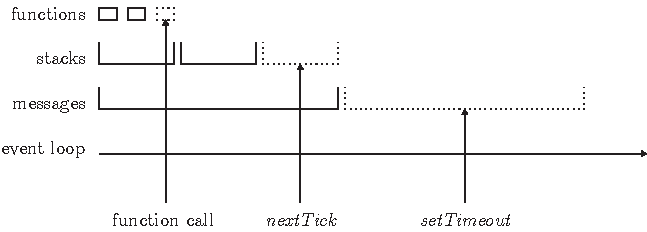
\includegraphics[width=\linewidth]{eventloop.pdf}
  \caption{Javascript event loop details}
  \label{fig:eventloop}
\end{figure}

\subsection{Three different implementations}

We tested our model with three different implementations.

\begin{itemize}
	\item[\textbf{Chain}]
		This implementation chains fluxions one after another by a direct function call.
		The whole fluxion chain is contain inside a same stack on Figure \ref{fig:eventloop}.
		It set the fluxions chain length maximum to the macimum function call stack size, and it's impossible to interleave messages from network in the middle of a fluxion chain.

	\item[\textbf{NextTick}]
		This implementation uses the instruction \texttt{process.nextTick} to chain fluxions execution.
		This instruction add a function call at the end of the current execution.
		Two local fluxion processing chain could run concurrently, but it's only possible to probe network messages every \textit{n} fluxions execution.
		By default \textit{n} is set to 1000.

	\item[\textbf{SetTimeout}]
		This implementation uses the instruction \texttt{setTimeout}.
		It probes network messages after every fluxion execution, thus networks messages can be interleaved between each local messages.
\end{itemize}

With these differents implementations, we want to highlight the advantages and drawbacks of the fluxionnal execution model.

% \begin{figure}
% \begin{tikzpicture}
\begin{axis}[ybar, ylabel={Average response time}, nodes near coords, nodes near coords align={vertical}, xtick=data, x tick label style={rotate=45,anchor=east}, symbolic x coords={chain, basic, nextTick, setTimeout}]
\addplot[color=black]
coordinates {(chain,30542.77957)(basic,55281.24429)(nextTick,80505.31194)(setTimeout,156418.66783)};
\end{axis}
\end{tikzpicture}

% \caption{Average response time for each implementation - 100 parallel clients, sequentillay connecting 1000 times}
% \label{fig:reponsetime}
% \end{figure}

% \begin{figure}
% \begin{tikzpicture}
\begin{semilogxaxis}[xmin=0,xmax=1000000, ylabel=Number of client, xlabel=Response time (ms)]
\addplot[color=blue, mark=x] coordinates {(6900,1)(9700,1)(10800,1)(11500,1)(11900,2)(12100,1)(12300,3)(12400,4)(12500,15)(12600,11)(12700,12)(12800,43)(12900,39)(13000,33)(13100,37)(13200,62)(13300,49)(13400,72)(13500,99)(13600,90)(13700,104)(13800,122)(13900,136)(14000,119)(14100,104)(14200,175)(14300,110)(14400,119)(14500,185)(14600,173)(14700,159)(14800,192)(14900,208)(15000,197)(15100,259)(15200,238)(15300,225)(15400,298)(15500,316)(15600,255)(15700,275)(15800,284)(15900,314)(16000,301)(16100,335)(16200,338)(16300,385)(16400,364)(16500,365)(16600,361)(16700,369)(16800,371)(16900,467)(17000,469)(17100,478)(17200,487)(17300,435)(17400,497)(17500,557)(17600,555)(17700,614)(17800,635)(17900,528)(18000,596)(18100,598)(18200,496)(18300,603)(18400,595)(18500,536)(18600,501)(18700,495)(18800,514)(18900,478)(19000,510)(19100,464)(19200,470)(19300,518)(19400,496)(19500,597)(19600,530)(19700,556)(19800,604)(19900,615)(20000,586)(20100,597)(20200,616)(20300,594)(20400,579)(20500,594)(20600,625)(20700,572)(20800,536)(20900,561)(21000,534)(21100,611)(21200,595)(21300,540)(21400,546)(21500,546)(21600,500)(21700,523)(21800,540)(21900,513)(22000,514)(22100,510)(22200,458)(22300,516)(22400,490)(22500,458)(22600,515)(22700,451)(22800,432)(22900,456)(23000,425)(23100,417)(23200,393)(23300,437)(23400,403)(23500,395)(23600,417)(23700,390)(23800,401)(23900,448)(24000,382)(24100,367)(24200,389)(24300,388)(24400,438)(24500,431)(24600,425)(24700,441)(24800,435)(24900,412)(25000,396)(25100,368)(25200,366)(25300,415)(25400,386)(25500,358)(25600,367)(25700,328)(25800,341)(25900,306)(26000,315)(26100,332)(26200,306)(26300,276)(26400,267)(26500,298)(26600,279)(26700,281)(26800,261)(26900,291)(27000,261)(27100,265)(27200,264)(27300,278)(27400,272)(27500,296)(27600,252)(27700,282)(27800,304)(27900,314)(28000,220)(28100,257)(28200,242)(28300,227)(28400,254)(28500,255)(28600,244)(28700,215)(28800,228)(28900,224)(29000,220)(29100,239)(29200,257)(29300,287)(29400,279)(29500,229)(29600,238)(29700,248)(29800,242)(29900,262)(30000,282)(30100,227)(30200,234)(30300,266)(30400,229)(30500,267)(30600,285)(30700,248)(30800,270)(30900,253)(31000,250)(31100,297)(31200,290)(31300,260)(31400,256)(31500,229)(31600,226)(31700,247)(31800,225)(31900,252)(32000,218)(32100,239)(32200,205)(32300,243)(32400,203)(32500,175)(32600,176)(32700,172)(32800,192)(32900,193)(33000,170)(33100,168)(33200,181)(33300,209)(33400,192)(33500,184)(33600,183)(33700,206)(33800,203)(33900,203)(34000,215)(34100,173)(34200,208)(34300,191)(34400,202)(34500,189)(34600,146)(34700,166)(34800,192)(34900,190)(35000,172)(35100,158)(35200,223)(35300,162)(35400,187)(35500,182)(35600,179)(35700,163)(35800,169)(35900,153)(36000,161)(36100,118)(36200,127)(36300,156)(36400,155)(36500,133)(36600,142)(36700,169)(36800,151)(36900,179)(37000,156)(37100,146)(37200,142)(37300,146)(37400,182)(37500,175)(37600,199)(37700,179)(37800,155)(37900,165)(38000,156)(38100,182)(38200,135)(38300,156)(38400,144)(38500,157)(38600,152)(38700,140)(38800,158)(38900,146)(39000,119)(39100,134)(39200,118)(39300,112)(39400,139)(39500,124)(39600,137)(39700,132)(39800,116)(39900,153)(40000,132)(40100,146)(40200,137)(40300,132)(40400,127)(40500,133)(40600,133)(40700,131)(40800,112)(40900,136)(41000,119)(41100,124)(41200,145)(41300,117)(41400,127)(41500,121)(41600,150)(41700,101)(41800,142)(41900,110)(42000,107)(42100,129)(42200,108)(42300,133)(42400,117)(42500,128)(42600,123)(42700,115)(42800,126)(42900,126)(43000,126)(43100,134)(43200,130)(43300,162)(43400,105)(43500,112)(43600,139)(43700,163)(43800,99)(43900,99)(44000,120)(44100,110)(44200,104)(44300,92)(44400,108)(44500,117)(44600,112)(44700,105)(44800,80)(44900,114)(45000,111)(45100,98)(45200,110)(45300,102)(45400,115)(45500,83)(45600,94)(45700,95)(45800,98)(45900,114)(46000,90)(46100,93)(46200,50)(46300,75)(46400,75)(46500,64)(46600,63)(46700,70)(46800,70)(46900,85)(47000,74)(47100,82)(47200,84)(47300,58)(47400,65)(47500,67)(47600,68)(47700,60)(47800,71)(47900,68)(48000,66)(48100,55)(48200,65)(48300,59)(48400,66)(48500,57)(48600,58)(48700,57)(48800,55)(48900,52)(49000,60)(49100,65)(49200,64)(49300,58)(49400,79)(49500,59)(49600,49)(49700,61)(49800,51)(49900,42)(50000,59)(50100,69)(50200,59)(50300,54)(50400,59)(50500,60)(50600,61)(50700,53)(50800,70)(50900,71)(51000,59)(51100,61)(51200,57)(51300,59)(51400,48)(51500,59)(51600,56)(51700,58)(51800,44)(51900,51)(52000,56)(52100,49)(52200,47)(52300,57)(52400,66)(52500,35)(52600,44)(52700,48)(52800,48)(52900,38)(53000,57)(53100,50)(53200,51)(53300,50)(53400,50)(53500,41)(53600,45)(53700,50)(53800,51)(53900,31)(54000,35)(54100,44)(54200,36)(54300,35)(54400,42)(54500,35)(54600,48)(54700,37)(54800,23)(54900,29)(55000,42)(55100,36)(55200,52)(55300,32)(55400,48)(55500,55)(55600,48)(55700,48)(55800,33)(55900,33)(56000,50)(56100,54)(56200,37)(56300,49)(56400,42)(56500,51)(56600,39)(56700,42)(56800,40)(56900,42)(57000,32)(57100,39)(57200,59)(57300,50)(57400,51)(57500,42)(57600,32)(57700,49)(57800,34)(57900,41)(58000,39)(58100,36)(58200,34)(58300,48)(58400,33)(58500,35)(58600,38)(58700,34)(58800,33)(58900,38)(59000,33)(59100,32)(59200,33)(59300,30)(59400,30)(59500,40)(59600,52)(59700,42)(59800,38)(59900,34)(60000,29)(60100,40)(60200,28)(60300,31)(60400,29)(60500,35)(60600,38)(60700,24)(60800,23)(60900,34)(61000,32)(61100,28)(61200,19)(61300,20)(61400,25)(61500,28)(61600,12)(61700,25)(61800,24)(61900,9)(62000,17)(62100,16)(62200,18)(62300,17)(62400,22)(62500,19)(62600,17)(62700,16)(62800,14)(62900,17)(63000,11)(63100,14)(63200,16)(63300,15)(63400,17)(63500,10)(63600,9)(63700,10)(63800,9)(63900,13)(64000,13)(64100,10)(64200,23)(64300,13)(64400,10)(64500,8)(64600,13)(64700,16)(64800,14)(64900,7)(65000,12)(65100,19)(65200,18)(65300,13)(65400,16)(65500,13)(65600,15)(65700,14)(65800,12)(65900,15)(66000,12)(66100,10)(66200,19)(66300,15)(66400,14)(66500,10)(66600,16)(66700,12)(66800,11)(66900,12)(67000,13)(67100,16)(67200,8)(67300,11)(67400,9)(67500,7)(67600,9)(67700,8)(67800,4)(67900,5)(68000,1)(68100,8)(68200,6)(68300,4)(68400,6)(68500,5)(68600,5)(68700,8)(68800,5)(68900,3)(69000,8)(69100,6)(69200,1)(69300,7)(69400,6)(69500,7)(69600,3)(69700,6)(69800,12)(69900,9)(70000,7)(70100,5)(70200,7)(70300,13)(70400,5)(70500,5)(70600,6)(70700,5)(70800,3)(70900,10)(71000,7)(71100,14)(71200,5)(71300,9)(71400,5)(71500,7)(71600,8)(71700,10)(71800,8)(71900,6)(72000,3)(72100,5)(72200,2)(72300,7)(72400,5)(72500,8)(72600,3)(72700,7)(72800,8)(72900,5)(73000,11)(73100,10)(73200,18)(73300,13)(73400,7)(73500,7)(73600,7)(73700,2)(73800,4)(73900,6)(74000,7)(74100,5)(74200,5)(74300,2)(74400,3)(74500,3)(74600,5)(74700,1)(74800,7)(74900,2)(75000,3)(75100,3)(75200,2)(75300,6)(75400,2)(75500,6)(75600,4)(75700,2)(75800,6)(75900,7)(76000,4)(76100,3)(76200,6)(76300,5)(76400,1)(76500,5)(76600,6)(76700,3)(76800,5)(76900,5)(77000,8)(77100,5)(77200,5)(77300,3)(77400,4)(77500,8)(77600,3)(77700,2)(77800,5)(77900,6)(78000,14)(78100,4)(78200,7)(78300,14)(78400,16)(78500,17)(78600,10)(78700,18)(78800,10)(78900,12)(79000,13)(79100,7)(79200,14)(79300,13)(79400,16)(79500,17)(79600,12)(79700,26)(79800,18)(79900,8)(80000,14)(80100,14)(80200,10)(80300,12)(80400,15)(80500,16)(80600,11)(80700,13)(80800,8)(80900,12)(81000,7)(81100,9)(81200,6)(81300,9)(81400,16)(81500,9)(81600,9)(81700,3)(81800,10)(81900,7)(82000,11)(82100,9)(82200,8)(82300,13)(82400,11)(82500,9)(82600,7)(82700,8)(82800,10)(82900,8)(83000,3)(83100,8)(83200,6)(83300,3)(83400,5)(83500,8)(83600,6)(83700,11)(83800,8)(83900,6)(84000,4)(84100,7)(84200,7)(84300,8)(84400,5)(84500,1)(84600,3)(84700,7)(84800,2)(84900,5)(85000,9)(85100,3)(85200,7)(85300,5)(85400,9)(85500,6)(85600,9)(85700,6)(85800,6)(85900,10)(86000,5)(86100,10)(86200,7)(86300,5)(86400,7)(86500,11)(86600,11)(86700,5)(86800,13)(86900,7)(87000,11)(87100,3)(87200,6)(87300,6)(87400,6)(87500,10)(87600,5)(87700,5)(87800,5)(87900,5)(88000,6)(88100,6)(88200,4)(88300,2)(88400,6)(88500,7)(88600,6)(88700,3)(88800,5)(88900,3)(89000,7)(89100,4)(89200,2)(89300,4)(89400,8)(89500,7)(89600,2)(89700,3)(89800,9)(89900,7)(90000,5)(90100,8)(90200,11)(90300,3)(90400,10)(90500,3)(90600,4)(90700,10)(90800,5)(90900,7)(91000,9)(91100,6)(91200,7)(91300,9)(91400,3)(91500,4)(91600,4)(91700,4)(91800,4)(91900,4)(92000,2)(92100,2)(92200,5)(92300,3)(92400,4)(92500,3)(92600,2)(92700,2)(92800,2)(92900,2)(93000,2)(93100,7)(93200,11)(93300,3)(93400,6)(93500,7)(93600,8)(93700,10)(93800,6)(93900,8)(94000,8)(94100,10)(94200,5)(94300,4)(94400,11)(94500,13)(94600,8)(94700,8)(94800,9)(94900,6)(95000,9)(95100,6)(95200,4)(95300,5)(95400,5)(95500,3)(95600,1)(95700,1)(95900,1)(96000,1)(96100,3)(96200,3)(96300,1)(96500,1)(96600,2)(96700,2)(96900,2)(97100,1)(97700,2)(97800,1)(98000,2)(98200,1)(98300,1)(98400,1)(98700,2)(98800,1)(99100,1)(99200,3)(99400,2)(99500,2)(99900,2)(100000,1)(100200,2)(100400,2)(100500,1)(100800,1)(100900,3)(101000,1)(101100,1)(101200,2)(101500,3)(101600,1)(101700,1)(101900,2)(102400,1)(103100,1)(103500,1)(103800,1)(104300,1)(104500,1)(105200,1)(105300,2)(105500,1)(105600,1)(106400,1)(106500,2)(106600,3)(106800,1)(106900,1)(107200,1)(107400,2)(107500,4)(107600,1)(107700,5)(107800,2)(107900,3)(108000,2)(108100,2)(108200,1)(108300,1)(108400,2)(108500,3)(108600,2)(108700,2)(108800,1)(108900,4)(109000,2)(109200,1)(109300,1)(109700,1)(110000,2)(110100,4)(110300,1)(110500,1)(110600,2)(110700,2)(110800,1)(111200,1)(111300,1)(111400,1)(111500,1)(111600,1)(111700,3)(111900,1)(112700,2)(114500,2)(114600,1)(115400,1)(132400,1)(132500,1)(133000,2)(133200,1)(136700,1)(137000,1)(138100,1)(138300,1)(138400,1)(138500,2)(138600,2)(138700,3)(138800,7)(139000,3)(139100,1)(139200,1)(139400,1)(139500,3)(139600,5)(139700,1)(139800,1)(140000,1)(140300,1)(140500,2)(140600,4)(140800,4)(140900,2)(141000,5)(141200,1)(141300,2)(141400,1)(141500,1)(141600,3)(141700,1)(141800,1)(141900,1)(142100,1)(142400,1)(142500,1)(142900,1)(143000,1)(143100,1)(143200,3)(143500,1)(143600,2)(143700,1)(143900,1)(144000,1)(144200,2)(144300,1)(144400,1)(144500,1)(144600,2)(144700,1)(144800,2)(144900,1)(145000,2)(145100,6)(145200,2)(145300,13)(145400,5)(145500,5)(145600,3)(145700,3)(145800,4)(145900,3)(146000,7)(146100,5)(146200,3)(146300,2)(146400,3)(146500,1)(146600,1)(146700,3)(146900,2)(147000,3)(147100,1)(147300,1)(147400,1)(147600,3)(147700,3)(147800,3)(147900,2)(148000,3)(148100,2)(148200,1)(148400,3)(148500,1)(148600,1)(148700,3)(153200,3)(153300,2)(154000,1)(154200,1)(154700,1)(197500,2)(197600,1)(198100,1)(238600,1)(238900,1)(239200,1)(278700,1)(278800,1)(279500,1)(283900,1)(284000,1)(284200,1)(284300,1)(284500,1)(284800,1)(285200,1)(285500,1)(318700,1)(319100,1)(319300,1)(319400,1)(398500,1)(398700,2)(398900,2)(399100,1)(399300,1)(399500,1)(399600,1)(399800,4)(400200,3)(400300,6)(400400,4)(400600,1)(400700,2)(400900,1)(401000,1)(401100,1)(401300,2)(401400,3)(401500,1)(401600,1)(401800,2)(402100,1)(402200,2)(402400,1)(402500,4)(402800,1)(402900,1)(403000,1)(403500,1)(403800,1)(404200,1)(405500,1)(406300,2)(406500,1)(407200,1)(407400,2)(407600,1)(407900,1)(408000,1)(408100,1)(408600,1)(408700,1)(409000,1)(409300,1)(409600,3)(410600,1)(411100,1)(411300,1)(411500,1)(412100,1)(412300,1)(412500,1)(412700,1)(413400,1)(414100,1)(414800,1)(415500,1)(416300,1)(416400,3)(416500,1)(416600,1)(416800,1)(416900,1)(417500,1)(418100,1)(418300,1)(495600,1)(495900,1)(496300,5)(496400,3)(496500,6)(496600,5)(496700,2)(496800,8)(496900,5)(497100,5)(497200,4)(497300,5)(497400,3)(497500,8)(497600,13)(497700,2)(497800,2)(497900,2)(498000,1)(498100,1)(498200,1)(498300,2)(498400,3)(498500,1)};
\addplot[color=red, mark=x] coordinates {(8000,3)(8200,1)(8600,1)(9100,1)(9300,1)(9400,1)(9600,1)(9700,2)(10000,1)(11300,2)(11500,2)(11800,1)(12100,1)(12400,5)(12500,7)(12600,2)(12700,12)(12800,46)(12900,63)(13000,54)(13100,80)(13200,104)(13300,113)(13400,162)(13500,177)(13600,216)(13700,242)(13800,268)(13900,317)(14000,329)(14100,401)(14200,450)(14300,430)(14400,460)(14500,504)(14600,522)(14700,527)(14800,523)(14900,501)(15000,568)(15100,598)(15200,513)(15300,568)(15400,558)(15500,524)(15600,555)(15700,519)(15800,594)(15900,468)(16000,523)(16100,511)(16200,574)(16300,567)(16400,653)(16500,597)(16600,704)(16700,723)(16800,699)(16900,636)(17000,672)(17100,701)(17200,633)(17300,656)(17400,665)(17500,651)(17600,642)(17700,668)(17800,729)(17900,662)(18000,672)(18100,705)(18200,698)(18300,677)(18400,616)(18500,574)(18600,655)(18700,635)(18800,604)(18900,590)(19000,593)(19100,607)(19200,566)(19300,620)(19400,554)(19500,603)(19600,611)(19700,694)(19800,604)(19900,584)(20000,616)(20100,622)(20200,587)(20300,624)(20400,658)(20500,659)(20600,686)(20700,750)(20800,709)(20900,722)(21000,681)(21100,648)(21200,695)(21300,647)(21400,681)(21500,673)(21600,691)(21700,662)(21800,630)(21900,670)(22000,566)(22100,652)(22200,664)(22300,620)(22400,662)(22500,589)(22600,560)(22700,545)(22800,594)(22900,537)(23000,517)(23100,556)(23200,520)(23300,507)(23400,529)(23500,452)(23600,501)(23700,455)(23800,470)(23900,471)(24000,503)(24100,465)(24200,428)(24300,414)(24400,407)(24500,396)(24600,390)(24700,401)(24800,393)(24900,366)(25000,375)(25100,338)(25200,354)(25300,317)(25400,300)(25500,291)(25600,295)(25700,334)(25800,335)(25900,306)(26000,320)(26100,318)(26200,287)(26300,290)(26400,254)(26500,293)(26600,270)(26700,235)(26800,226)(26900,245)(27000,238)(27100,235)(27200,261)(27300,264)(27400,263)(27500,252)(27600,282)(27700,238)(27800,267)(27900,290)(28000,264)(28100,267)(28200,252)(28300,255)(28400,275)(28500,242)(28600,251)(28700,264)(28800,249)(28900,231)(29000,248)(29100,259)(29200,229)(29300,206)(29400,194)(29500,202)(29600,212)(29700,212)(29800,180)(29900,187)(30000,185)(30100,188)(30200,170)(30300,156)(30400,211)(30500,174)(30600,187)(30700,182)(30800,186)(30900,181)(31000,196)(31100,172)(31200,164)(31300,184)(31400,196)(31500,191)(31600,203)(31700,154)(31800,172)(31900,186)(32000,195)(32100,188)(32200,177)(32300,193)(32400,161)(32500,151)(32600,172)(32700,171)(32800,198)(32900,163)(33000,173)(33100,166)(33200,184)(33300,143)(33400,141)(33500,162)(33600,135)(33700,163)(33800,150)(33900,144)(34000,101)(34100,161)(34200,131)(34300,152)(34400,132)(34500,120)(34600,102)(34700,110)(34800,137)(34900,116)(35000,118)(35100,92)(35200,122)(35300,86)(35400,84)(35500,81)(35600,97)(35700,114)(35800,100)(35900,104)(36000,105)(36100,94)(36200,110)(36300,110)(36400,121)(36500,121)(36600,100)(36700,115)(36800,119)(36900,95)(37000,106)(37100,115)(37200,112)(37300,112)(37400,100)(37500,78)(37600,90)(37700,86)(37800,84)(37900,113)(38000,92)(38100,78)(38200,82)(38300,53)(38400,67)(38500,64)(38600,76)(38700,82)(38800,77)(38900,83)(39000,69)(39100,58)(39200,50)(39300,53)(39400,75)(39500,70)(39600,65)(39700,77)(39800,83)(39900,67)(40000,62)(40100,77)(40200,72)(40300,86)(40400,86)(40500,84)(40600,76)(40700,67)(40800,71)(40900,78)(41000,81)(41100,74)(41200,63)(41300,82)(41400,61)(41500,78)(41600,69)(41700,86)(41800,63)(41900,38)(42000,64)(42100,79)(42200,39)(42300,64)(42400,72)(42500,77)(42600,68)(42700,57)(42800,82)(42900,52)(43000,56)(43100,66)(43200,59)(43300,51)(43400,57)(43500,43)(43600,49)(43700,45)(43800,70)(43900,43)(44000,43)(44100,54)(44200,55)(44300,52)(44400,41)(44500,29)(44600,37)(44700,74)(44800,43)(44900,40)(45000,46)(45100,43)(45200,40)(45300,51)(45400,40)(45500,50)(45600,48)(45700,41)(45800,58)(45900,40)(46000,46)(46100,34)(46200,43)(46300,50)(46400,36)(46500,55)(46600,40)(46700,40)(46800,40)(46900,36)(47000,36)(47100,23)(47200,36)(47300,40)(47400,48)(47500,36)(47600,28)(47700,40)(47800,40)(47900,38)(48000,47)(48100,26)(48200,31)(48300,41)(48400,37)(48500,42)(48600,35)(48700,45)(48800,38)(48900,31)(49000,36)(49100,47)(49200,30)(49300,37)(49400,32)(49500,36)(49600,27)(49700,20)(49800,22)(49900,23)(50000,26)(50100,28)(50200,28)(50300,26)(50400,34)(50500,47)(50600,33)(50700,27)(50800,32)(50900,27)(51000,26)(51100,17)(51200,26)(51300,29)(51400,23)(51500,25)(51600,29)(51700,29)(51800,28)(51900,27)(52000,27)(52100,13)(52200,19)(52300,26)(52400,19)(52500,21)(52600,42)(52700,33)(52800,27)(52900,29)(53000,29)(53100,33)(53200,29)(53300,36)(53400,30)(53500,35)(53600,37)(53700,30)(53800,33)(53900,23)(54000,23)(54100,28)(54200,26)(54300,28)(54400,42)(54500,31)(54600,59)(54700,25)(54800,22)(54900,31)(55000,14)(55100,13)(55200,9)(55300,22)(55400,29)(55500,26)(55600,11)(55700,15)(55800,31)(55900,22)(56000,19)(56100,17)(56200,17)(56300,30)(56400,15)(56500,12)(56600,19)(56700,22)(56800,26)(56900,21)(57000,25)(57100,20)(57200,15)(57300,19)(57400,19)(57500,17)(57600,17)(57700,21)(57800,19)(57900,17)(58000,10)(58100,12)(58200,16)(58300,21)(58400,13)(58500,7)(58600,10)(58700,9)(58800,15)(58900,14)(59000,6)(59100,6)(59200,10)(59300,12)(59400,10)(59500,11)(59600,9)(59700,7)(59800,6)(59900,12)(60000,12)(60100,11)(60200,8)(60300,10)(60400,16)(60500,9)(60600,12)(60700,11)(60800,8)(60900,11)(61000,7)(61100,7)(61200,8)(61300,8)(61400,10)(61500,22)(61600,15)(61700,9)(61800,7)(61900,13)(62000,10)(62100,8)(62200,3)(62300,6)(62400,3)(62500,10)(62600,6)(62700,6)(62800,5)(62900,4)(63000,2)(63100,3)(63200,4)(63300,1)(63400,8)(63500,3)(63600,4)(63700,2)(63800,5)(63900,9)(64000,4)(64100,3)(64200,7)(64300,7)(64400,5)(64500,6)(64600,5)(64700,5)(64800,5)(64900,1)(65000,2)(65100,6)(65200,3)(65300,10)(65400,9)(65500,5)(65600,10)(65700,4)(65800,2)(65900,5)(66000,1)(66100,2)(66200,4)(66300,5)(66400,4)(66500,2)(66600,3)(66700,6)(66800,5)(66900,4)(67000,3)(67100,4)(67200,4)(67300,6)(67400,3)(67500,3)(67600,2)(67800,2)(67900,2)(68000,3)(68100,3)(68200,1)(68400,1)(68500,4)(68600,7)(68800,4)(68900,3)(69000,3)(69100,1)(69200,5)(69300,4)(69400,2)(69500,3)(69600,2)(69800,3)(69900,3)(70200,3)(70300,3)(70400,2)(70500,3)(70600,6)(70700,5)(70800,2)(70900,5)(71000,5)(71100,3)(71200,1)(71300,6)(71400,2)(71500,3)(71600,4)(71700,6)(71800,7)(71900,5)(72000,7)(72100,2)(72200,5)(72300,3)(72400,9)(72500,1)(72600,5)(72700,7)(72800,8)(72900,3)(73000,3)(73100,5)(73200,9)(73300,7)(73400,1)(73500,2)(73600,2)(73700,3)(73800,3)(73900,5)(74000,1)(74100,9)(74200,5)(74300,3)(74400,3)(74500,2)(74600,1)(74700,1)(74800,2)(75000,6)(75100,3)(75200,1)(75300,4)(75400,2)(75500,4)(75600,5)(75700,1)(75800,2)(75900,2)(76000,5)(76200,1)(76400,5)(76500,3)(76600,2)(76700,2)(76800,2)(77000,3)(77100,2)(77200,1)(77400,1)(77500,3)(77600,2)(77700,1)(77800,1)(77900,2)(78000,3)(78100,2)(78200,1)(78300,1)(78400,1)(78500,1)(78700,2)(78800,6)(78900,2)(79000,2)(79100,5)(79200,5)(79300,5)(79400,1)(79500,6)(79600,3)(79700,2)(79800,3)(79900,3)(80100,6)(80300,1)(80500,1)(80700,1)(80800,2)(80900,1)(81000,2)(81200,3)(81300,1)(81400,2)(81500,1)(81600,1)(81700,1)(81900,2)(82000,2)(82200,1)(82300,1)(82500,1)(82600,1)(82800,1)(83000,1)(83100,1)(83200,1)(83300,1)(83400,1)(83600,2)(83900,2)(84300,3)(84700,2)(85000,2)(85400,2)(85500,3)(86300,1)(87100,1)(87600,2)(87900,1)(88100,1)(88200,1)(88500,1)(88900,1)(89300,2)(89700,1)(90000,1)(90100,2)(90200,2)(90600,2)(91000,2)(91200,2)(91300,1)(91400,2)(91600,4)(91700,1)(91800,1)(91900,1)(92000,2)(92200,1)(92400,1)(92600,1)(92700,1)(92800,1)(92900,1)(93000,1)(93200,1)(93300,1)(93400,2)(93500,1)(93600,1)(93700,1)(93800,1)(94100,1)(94200,1)(94300,1)(94500,1)(94600,2)(94700,1)(94800,1)(95300,2)};
\addplot[color=green, mark=x] coordinates {(7100,1)(7300,1)(7600,1)(7700,1)(7800,1)(10300,1)(11300,1)(11500,1)(11600,3)(11700,17)(11800,64)(11900,73)(12000,73)(12100,79)(12200,116)(12300,102)(12400,82)(12500,82)(12600,89)(12700,142)(12800,186)(12900,175)(13000,277)(13100,298)(13200,318)(13300,425)(13400,484)(13500,364)(13600,365)(13700,414)(13800,488)(13900,509)(14000,532)(14100,503)(14200,516)(14300,515)(14400,595)(14500,655)(14600,595)(14700,717)(14800,662)(14900,693)(15000,678)(15100,702)(15200,704)(15300,698)(15400,672)(15500,653)(15600,673)(15700,593)(15800,564)(15900,564)(16000,489)(16100,521)(16200,489)(16300,451)(16400,456)(16500,413)(16600,458)(16700,473)(16800,441)(16900,435)(17000,479)(17100,485)(17200,476)(17300,487)(17400,544)(17500,566)(17600,558)(17700,599)(17800,548)(17900,511)(18000,547)(18100,606)(18200,583)(18300,589)(18400,587)(18500,635)(18600,602)(18700,616)(18800,680)(18900,621)(19000,632)(19100,644)(19200,700)(19300,698)(19400,742)(19500,667)(19600,644)(19700,629)(19800,668)(19900,642)(20000,741)(20100,708)(20200,641)(20300,621)(20400,724)(20500,688)(20600,628)(20700,643)(20800,633)(20900,557)(21000,625)(21100,590)(21200,556)(21300,537)(21400,521)(21500,523)(21600,523)(21700,477)(21800,531)(21900,496)(22000,504)(22100,449)(22200,499)(22300,479)(22400,494)(22500,509)(22600,502)(22700,494)(22800,487)(22900,488)(23000,530)(23100,515)(23200,454)(23300,490)(23400,461)(23500,441)(23600,453)(23700,415)(23800,423)(23900,428)(24000,388)(24100,384)(24200,323)(24300,387)(24400,410)(24500,378)(24600,395)(24700,383)(24800,348)(24900,361)(25000,394)(25100,393)(25200,328)(25300,365)(25400,379)(25500,362)(25600,345)(25700,341)(25800,322)(25900,321)(26000,329)(26100,331)(26200,303)(26300,301)(26400,300)(26500,303)(26600,313)(26700,249)(26800,273)(26900,241)(27000,276)(27100,284)(27200,235)(27300,242)(27400,222)(27500,230)(27600,208)(27700,185)(27800,212)(27900,193)(28000,180)(28100,202)(28200,228)(28300,253)(28400,207)(28500,203)(28600,196)(28700,163)(28800,194)(28900,210)(29000,232)(29100,228)(29200,236)(29300,239)(29400,210)(29500,209)(29600,172)(29700,172)(29800,182)(29900,169)(30000,181)(30100,160)(30200,147)(30300,181)(30400,131)(30500,156)(30600,146)(30700,165)(30800,155)(30900,176)(31000,188)(31100,142)(31200,168)(31300,166)(31400,176)(31500,171)(31600,194)(31700,192)(31800,178)(31900,188)(32000,159)(32100,190)(32200,183)(32300,171)(32400,168)(32500,157)(32600,145)(32700,153)(32800,148)(32900,140)(33000,121)(33100,151)(33200,134)(33300,115)(33400,128)(33500,118)(33600,96)(33700,105)(33800,107)(33900,94)(34000,121)(34100,85)(34200,87)(34300,82)(34400,86)(34500,88)(34600,122)(34700,98)(34800,84)(34900,79)(35000,87)(35100,72)(35200,93)(35300,102)(35400,116)(35500,102)(35600,94)(35700,97)(35800,86)(35900,81)(36000,105)(36100,92)(36200,91)(36300,134)(36400,112)(36500,118)(36600,127)(36700,129)(36800,119)(36900,113)(37000,80)(37100,89)(37200,74)(37300,81)(37400,87)(37500,85)(37600,82)(37700,76)(37800,83)(37900,85)(38000,94)(38100,103)(38200,87)(38300,96)(38400,77)(38500,79)(38600,104)(38700,94)(38800,89)(38900,102)(39000,80)(39100,124)(39200,83)(39300,88)(39400,95)(39500,101)(39600,87)(39700,84)(39800,99)(39900,97)(40000,105)(40100,86)(40200,93)(40300,102)(40400,81)(40500,86)(40600,84)(40700,91)(40800,72)(40900,75)(41000,73)(41100,88)(41200,82)(41300,77)(41400,82)(41500,75)(41600,68)(41700,101)(41800,78)(41900,80)(42000,72)(42100,96)(42200,77)(42300,79)(42400,89)(42500,92)(42600,84)(42700,78)(42800,86)(42900,62)(43000,59)(43100,67)(43200,48)(43300,58)(43400,56)(43500,63)(43600,45)(43700,70)(43800,57)(43900,57)(44000,64)(44100,33)(44200,59)(44300,60)(44400,46)(44500,47)(44600,45)(44700,44)(44800,46)(44900,37)(45000,42)(45100,40)(45200,41)(45300,43)(45400,50)(45500,39)(45600,48)(45700,39)(45800,51)(45900,48)(46000,52)(46100,47)(46200,47)(46300,47)(46400,55)(46500,49)(46600,38)(46700,50)(46800,47)(46900,47)(47000,37)(47100,41)(47200,26)(47300,46)(47400,35)(47500,52)(47600,57)(47700,40)(47800,28)(47900,31)(48000,21)(48100,18)(48200,43)(48300,30)(48400,25)(48500,43)(48600,34)(48700,25)(48800,27)(48900,18)(49000,30)(49100,25)(49200,39)(49300,30)(49400,43)(49500,35)(49600,21)(49700,31)(49800,30)(49900,23)(50000,16)(50100,27)(50200,32)(50300,25)(50400,43)(50500,33)(50600,38)(50700,42)(50800,30)(50900,41)(51000,58)(51100,40)(51200,43)(51300,34)(51400,37)(51500,36)(51600,41)(51700,36)(51800,24)(51900,34)(52000,33)(52100,27)(52200,32)(52300,44)(52400,27)(52500,33)(52600,30)(52700,27)(52800,16)(52900,15)(53000,32)(53100,19)(53200,11)(53300,15)(53400,20)(53500,17)(53600,19)(53700,16)(53800,12)(53900,16)(54000,20)(54100,11)(54200,9)(54300,16)(54400,20)(54500,11)(54600,14)(54700,18)(54800,25)(54900,12)(55000,19)(55100,13)(55200,10)(55300,15)(55400,19)(55500,22)(55600,19)(55700,16)(55800,14)(55900,11)(56000,12)(56100,8)(56200,18)(56300,12)(56400,19)(56500,15)(56600,17)(56700,17)(56800,10)(56900,21)(57000,18)(57100,9)(57200,5)(57300,10)(57400,14)(57500,13)(57600,13)(57700,15)(57800,22)(57900,12)(58000,14)(58100,11)(58200,11)(58300,11)(58400,24)(58500,33)(58600,18)(58700,16)(58800,15)(58900,16)(59000,15)(59100,14)(59200,20)(59300,30)(59400,22)(59500,11)(59600,14)(59700,14)(59800,16)(59900,23)(60000,12)(60100,13)(60200,10)(60300,13)(60400,9)(60500,17)(60600,20)(60700,22)(60800,20)(60900,16)(61000,14)(61100,10)(61200,24)(61300,13)(61400,17)(61500,13)(61600,18)(61700,19)(61800,21)(61900,19)(62000,18)(62100,9)(62200,14)(62300,17)(62400,14)(62500,13)(62600,10)(62700,10)(62800,10)(62900,11)(63000,15)(63100,14)(63200,9)(63300,11)(63400,8)(63500,10)(63600,14)(63700,15)(63800,11)(63900,7)(64000,9)(64100,8)(64200,8)(64300,9)(64400,8)(64500,10)(64600,10)(64700,19)(64800,9)(64900,13)(65000,11)(65100,10)(65200,9)(65300,11)(65400,12)(65500,8)(65600,9)(65700,16)(65800,20)(65900,13)(66000,9)(66100,8)(66200,10)(66300,9)(66400,9)(66500,5)(66600,10)(66700,13)(66800,6)(66900,5)(67000,8)(67100,8)(67200,7)(67300,7)(67400,5)(67500,10)(67600,3)(67700,6)(67800,10)(67900,8)(68000,8)(68100,10)(68200,6)(68300,10)(68400,10)(68500,5)(68600,4)(68700,5)(68800,8)(68900,7)(69000,12)(69100,11)(69200,7)(69300,10)(69400,8)(69500,11)(69600,7)(69700,4)(69800,5)(69900,11)(70000,10)(70100,5)(70200,6)(70300,3)(70400,3)(70500,4)(70600,2)(70700,3)(70800,3)(70900,4)(71000,6)(71100,4)(71200,3)(71300,5)(71400,6)(71500,7)(71600,7)(71700,6)(71900,1)(72000,5)(72100,2)(72200,6)(72300,10)(72400,3)(72500,4)(72600,2)(72700,3)(72800,5)(73000,1)(73100,3)(73200,4)(73300,8)(73400,6)(73500,3)(73600,2)(73700,5)(73800,2)(73900,2)(74000,3)(74100,7)(74200,5)(74300,2)(74400,3)(74500,4)(74600,2)(74700,1)(74800,4)(74900,5)(75000,3)(75100,8)(75200,5)(75300,6)(75400,8)(75500,1)(75600,2)(75700,6)(75800,3)(75900,5)(76000,4)(76100,2)(76200,2)(76300,5)(76400,2)(76500,5)(76600,3)(76700,3)(76800,7)(76900,8)(77000,1)(77100,3)(77200,10)(77300,2)(77400,3)(77500,3)(77600,5)(77700,8)(77800,6)(77900,2)(78000,6)(78100,5)(78200,7)(78300,5)(78400,7)(78500,5)(78600,3)(78700,4)(78800,4)(78900,5)(79000,4)(79100,2)(79200,2)(79300,3)(79400,3)(79500,6)(79600,10)(79700,12)(79800,9)(79900,6)(80000,4)(80100,4)(80200,3)(80300,8)(80400,8)(80500,6)(80600,9)(80700,5)(80800,11)(80900,2)(81000,4)(81100,8)(81200,7)(81300,9)(81400,5)(81500,6)(81600,5)(81700,8)(81800,6)(81900,8)(82000,6)(82100,4)(82200,9)(82300,7)(82400,6)(82500,6)(82600,7)(82700,9)(82800,2)(82900,6)(83000,1)(83100,3)(83200,4)(83300,4)(83400,5)(83500,3)(83600,4)(83700,2)(83800,4)(83900,4)(84000,2)(84100,2)(84200,5)(84300,8)(84400,4)(84500,6)(84600,3)(84700,2)(84800,3)(85000,4)(85100,4)(85200,7)(85300,5)(85400,3)(85500,6)(85600,6)(85700,5)(85800,7)(85900,14)(86000,14)(86100,5)(86200,3)(86300,5)(86400,7)(86500,4)(86600,2)(86700,5)(86800,4)(86900,5)(87000,1)(87100,4)(87200,5)(87300,4)(87400,1)(87500,3)(87600,1)(87700,6)(87800,1)(87900,1)(88000,3)(88100,2)(88200,2)(88300,1)(88400,3)(88500,2)(88600,2)(88700,1)(88800,1)(89000,2)(89100,3)(89200,2)(89400,2)(89500,1)(89900,2)(90000,1)(90200,2)(90300,1)(90700,1)(141000,1)(141300,3)(141500,3)(141600,1)(141800,2)(141900,1)(142000,4)(142100,3)(142200,1)(142300,6)(142400,1)(142600,1)(142700,3)(142800,2)(142900,2)(143000,1)(143200,2)(143300,3)(143600,2)(143700,1)(143800,2)(144000,3)(144100,2)(144400,3)(144700,2)(144800,4)(144900,1)(145000,1)(145100,2)(145300,1)(145500,3)(145900,3)(146000,1)(146100,1)(146200,2)(146300,2)(146400,2)(146500,2)(146600,1)(146700,1)(146900,1)(147000,3)(147100,2)(147200,1)(147300,2)(147500,1)(147900,1)(166900,1)(167000,1)(167300,2)(167400,2)(167500,2)(167700,1)(167900,1)(168100,1)(168500,1)(168900,1)(169000,1)(263900,1)(264400,1)(264500,1)(264600,1)(265000,1)(265400,1)(265600,1)(281800,2)(282700,1)(283100,1)(298900,1)(299000,1)(299200,1)(299400,1)(299600,1)(299800,2)(299900,3)(300000,2)(300100,2)(300400,1)(300600,1)(300800,2)(300900,3)(301000,4)(301200,3)(301300,2)(301400,3)(301500,1)(301600,1)(301700,1)(301900,1)(302100,1)(302200,4)(302300,1)(302600,1)(303100,1)(305100,1)(305200,1)(305500,1)(305600,1)(305700,3)(306200,1)(306300,1)(306500,1)(306600,1)(306800,2)(307400,1)(307600,1)(308000,1)(308900,1)(310200,1)(310500,1)(310700,1)(311300,1)(311700,1)(313300,1)(313500,3)(313900,2)(314000,2)(314200,1)(314300,2)(314400,1)(315200,1)(315400,1)(315500,1)};
\addplot[color=yellow, mark=x] coordinates {(20000,1)(21000,1)(22000,1)(22300,1)(22600,1)(23000,1)(23500,1)(24800,1)(25000,1)(27100,1)(27400,1)(27600,1)(29300,1)(29500,1)(31200,1)(32100,1)(32300,1)(34100,1)(34300,1)(35900,1)(36100,1)(37100,1)(38500,1)(38800,1)(39800,1)(41600,1)(44600,1)(45100,1)(45500,1)(45700,1)(47500,1)(48500,1)(49800,1)(51500,1)(51700,2)(51800,1)(51900,3)(52000,7)(52100,1)(52200,1)(52300,8)(52600,1)(52700,8)(52800,4)(52900,10)(53000,11)(53100,8)(53200,7)(53300,7)(53400,4)(53500,3)(53600,5)(53700,12)(53800,8)(53900,8)(54000,16)(54100,14)(54200,24)(54300,39)(54400,5)(54500,7)(54600,4)(54700,3)(54800,2)(54900,3)(55000,8)(55100,16)(55200,9)(55300,4)(55400,21)(55500,17)(55600,19)(55700,9)(55800,8)(55900,9)(56000,8)(56100,13)(56200,8)(56300,7)(56400,6)(56500,14)(56600,9)(56700,6)(56800,10)(56900,14)(57000,10)(57100,8)(57200,17)(57300,7)(57400,7)(57500,12)(57600,7)(57700,8)(57800,18)(57900,14)(58000,18)(58100,16)(58200,16)(58300,3)(58400,15)(58500,10)(58600,11)(58700,15)(58800,7)(58900,8)(59000,8)(59100,16)(59200,21)(59300,19)(59400,24)(59500,15)(59600,20)(59700,16)(59800,27)(59900,31)(60000,39)(60100,24)(60200,30)(60300,17)(60400,25)(60500,26)(60600,15)(60700,25)(60800,26)(60900,31)(61000,23)(61100,27)(61200,32)(61300,20)(61400,17)(61500,30)(61600,36)(61700,33)(61800,30)(61900,35)(62000,25)(62100,24)(62200,25)(62300,29)(62400,41)(62500,51)(62600,39)(62700,66)(62800,49)(62900,43)(63000,41)(63100,59)(63200,59)(63300,63)(63400,48)(63500,42)(63600,52)(63700,54)(63800,72)(63900,54)(64000,66)(64100,79)(64200,81)(64300,106)(64400,106)(64500,100)(64600,76)(64700,78)(64800,103)(64900,110)(65000,91)(65100,100)(65200,110)(65300,84)(65400,95)(65500,123)(65600,117)(65700,146)(65800,176)(65900,159)(66000,160)(66100,167)(66200,182)(66300,203)(66400,146)(66500,182)(66600,151)(66700,168)(66800,167)(66900,180)(67000,221)(67100,195)(67200,215)(67300,170)(67400,201)(67500,174)(67600,183)(67700,190)(67800,187)(67900,188)(68000,260)(68100,266)(68200,267)(68300,276)(68400,281)(68500,277)(68600,275)(68700,251)(68800,269)(68900,310)(69000,319)(69100,285)(69200,310)(69300,311)(69400,304)(69500,336)(69600,337)(69700,385)(69800,381)(69900,387)(70000,431)(70100,368)(70200,414)(70300,410)(70400,387)(70500,426)(70600,399)(70700,385)(70800,455)(70900,431)(71000,429)(71100,483)(71200,495)(71300,475)(71400,459)(71500,471)(71600,484)(71700,517)(71800,498)(71900,532)(72000,496)(72100,592)(72200,577)(72300,647)(72400,544)(72500,556)(72600,518)(72700,541)(72800,584)(72900,593)(73000,628)(73100,639)(73200,641)(73300,762)(73400,696)(73500,662)(73600,663)(73700,705)(73800,701)(73900,667)(74000,761)(74100,838)(74200,744)(74300,773)(74400,876)(74500,842)(74600,942)(74700,856)(74800,862)(74900,955)(75000,865)(75100,838)(75200,944)(75300,872)(75400,847)(75500,842)(75600,932)(75700,835)(75800,928)(75900,931)(76000,891)(76100,867)(76200,1004)(76300,897)(76400,938)(76500,852)(76600,778)(76700,948)(76800,885)(76900,960)(77000,973)(77100,933)(77200,798)(77300,800)(77400,750)(77500,743)(77600,732)(77700,741)(77800,667)(77900,661)(78000,618)(78100,669)(78200,695)(78300,641)(78400,611)(78500,633)(78600,637)(78700,661)(78800,580)(78900,579)(79000,619)(79100,550)(79200,536)(79300,522)(79400,485)(79500,477)(79600,498)(79700,461)(79800,456)(79900,520)(80000,452)(80100,512)(80200,466)(80300,418)(80400,420)(80500,371)(80600,394)(80700,359)(80800,364)(80900,366)(81000,363)(81100,343)(81200,331)(81300,319)(81400,310)(81500,323)(81600,318)(81700,289)(81800,281)(81900,281)(82000,278)(82100,281)(82200,212)(82300,244)(82400,201)(82500,178)(82600,190)(82700,188)(82800,190)(82900,169)(83000,188)(83100,180)(83200,166)(83300,128)(83400,124)(83500,121)(83600,164)(83700,135)(83800,131)(83900,132)(84000,103)(84100,109)(84200,115)(84300,152)(84400,128)(84500,123)(84600,117)(84700,122)(84800,121)(84900,115)(85000,120)(85100,86)(85200,93)(85300,109)(85400,127)(85500,103)(85600,81)(85700,91)(85800,108)(85900,111)(86000,102)(86100,97)(86200,90)(86300,68)(86400,81)(86500,78)(86600,80)(86700,86)(86800,92)(86900,66)(87000,64)(87100,48)(87200,64)(87300,60)(87400,68)(87500,53)(87600,69)(87700,51)(87800,54)(87900,59)(88000,76)(88100,54)(88200,65)(88300,57)(88400,58)(88500,40)(88600,53)(88700,56)(88800,60)(88900,41)(89000,42)(89100,47)(89200,58)(89300,64)(89400,49)(89500,63)(89600,62)(89700,45)(89800,75)(89900,50)(90000,58)(90100,77)(90200,43)(90300,70)(90400,53)(90500,46)(90600,47)(90700,55)(90800,53)(90900,47)(91000,27)(91100,44)(91200,43)(91300,30)(91400,57)(91500,39)(91600,52)(91700,49)(91800,38)(91900,53)(92000,50)(92100,29)(92200,37)(92300,37)(92400,31)(92500,30)(92600,33)(92700,39)(92800,37)(92900,44)(93000,38)(93100,38)(93200,28)(93300,45)(93400,38)(93500,30)(93600,24)(93700,18)(93800,23)(93900,21)(94000,29)(94100,24)(94200,31)(94300,33)(94400,26)(94500,21)(94600,27)(94700,29)(94800,25)(94900,12)(95000,20)(95100,24)(95200,15)(95300,18)(95400,16)(95500,21)(95600,18)(95700,22)(95800,34)(95900,20)(96000,16)(96100,14)(96200,15)(96300,22)(96400,12)(96500,11)(96600,8)(96700,14)(96800,11)(96900,16)(97000,14)(97100,16)(97200,12)(97300,22)(97400,19)(97500,17)(97600,12)(97700,9)(97800,11)(97900,16)(98000,12)(98100,10)(98200,11)(98300,10)(98400,9)(98500,7)(98600,6)(98700,2)(98800,9)(98900,4)(99000,4)(99100,4)(99200,7)(99300,4)(99400,6)(99500,6)(99600,10)(99700,14)(99800,7)(99900,4)(100000,6)(100100,6)(100200,8)(100300,4)(100400,4)(100500,4)(100600,6)(100700,8)(100800,6)(100900,9)(101000,7)(101100,2)(101300,4)(101400,1)(101500,11)(101600,5)(101700,5)(101800,6)(101900,12)(102000,6)(102100,6)(102200,5)(102300,5)(102400,6)(102500,7)(102600,5)(102700,8)(102800,4)(102900,5)(103000,2)(103100,7)(103200,7)(103300,3)(103400,9)(103500,8)(103600,7)(103700,4)(103800,4)(103900,2)(104000,5)(104100,4)(104200,3)(104300,2)(104400,2)(104500,2)(104600,3)(104700,5)(104800,8)(104900,6)(105000,5)(105100,3)(105200,7)(105300,6)(105400,6)(105500,4)(105600,1)(105700,5)(105800,7)(105900,10)(106000,6)(106100,16)(106200,7)(106300,5)(106400,6)(106500,6)(106600,3)(106700,2)(106800,3)(106900,6)(107000,6)(107100,8)(107200,8)(107300,2)(107400,4)(107500,5)(107600,4)(107700,7)(107800,5)(107900,5)(108000,8)(108100,4)(108200,5)(108300,9)(108400,2)(108500,4)(108600,7)(108700,4)(108800,11)(108900,7)(109000,4)(109100,5)(109200,3)(109300,3)(109500,1)(109600,3)(109700,2)(109800,5)(109900,4)(110000,4)(110200,1)(110400,1)(110500,1)(110600,1)(110700,1)(110800,2)(110900,2)(111000,2)(111200,1)(111300,2)(111500,1)(111600,4)(111700,2)(111800,3)(111900,1)(112000,1)(112100,2)(112200,3)(112300,3)(112500,5)(112700,3)(112800,3)(112900,5)(113000,2)(113100,2)(113300,2)(113400,2)(113500,1)(113600,1)(113700,2)(113800,2)(113900,3)(114000,3)(114100,1)(114300,1)(114600,1)(114700,2)(115000,1)(115200,1)(115300,1)(115400,1)(115500,3)(115600,1)(115800,1)(116200,1)(116400,1)(116500,1)(116600,2)(117000,1)(117100,1)(117300,1)(118100,1)(118300,1)(118600,1)(118800,1)(118900,1)(119000,3)(119100,1)(120100,1)(120300,2)(120400,3)(120500,1)(120600,3)(120800,1)(121000,3)(121100,3)(121200,1)(121300,1)(121400,1)(121600,2)(122000,2)(122200,1)(122500,2)(122700,1)(122900,1)(123000,1)(123400,1)(123900,1)(124600,2)(124900,1)(125500,1)(125600,1)(125700,1)(126000,1)(126500,1)(126700,1)(126900,1)(127100,1)(128200,1)(128300,1)};
\legend{chain, basic, nextTick, setTimeout}
\end{semilogxaxis}
\end{tikzpicture}

% \caption{Distribution of response time for each implementation - 100 parallel clients, sequentillay connecting 1000 times}
% \label{fig:distribution}
% \end{figure}

% \begin{figure}
% \begin{tikzpicture}
\begin{semilogxaxis}[xmin=0,xmax=1000000, ylabel=Number of client, xlabel=Response time (ms)]

\addplot[color=black, mark=x] coordinates {(8000,3)(8200,1)(8600,1)(9100,1)(9300,1)(9400,1)(9600,1)(9700,2)(10000,1)(11300,2)(11500,2)(11800,1)(12100,1)(12400,5)(12500,7)(12600,2)(12700,12)(12800,46)(12900,63)(13000,54)(13100,80)(13200,104)(13300,113)(13400,162)(13500,177)(13600,216)(13700,242)(13800,268)(13900,317)(14000,329)(14100,401)(14200,450)(14300,430)(14400,460)(14500,504)(14600,522)(14700,527)(14800,523)(14900,501)(15000,568)(15100,598)(15200,513)(15300,568)(15400,558)(15500,524)(15600,555)(15700,519)(15800,594)(15900,468)(16000,523)(16100,511)(16200,574)(16300,567)(16400,653)(16500,597)(16600,704)(16700,723)(16800,699)(16900,636)(17000,672)(17100,701)(17200,633)(17300,656)(17400,665)(17500,651)(17600,642)(17700,668)(17800,729)(17900,662)(18000,672)(18100,705)(18200,698)(18300,677)(18400,616)(18500,574)(18600,655)(18700,635)(18800,604)(18900,590)(19000,593)(19100,607)(19200,566)(19300,620)(19400,554)(19500,603)(19600,611)(19700,694)(19800,604)(19900,584)(20000,616)(20100,622)(20200,587)(20300,624)(20400,658)(20500,659)(20600,686)(20700,750)(20800,709)(20900,722)(21000,681)(21100,648)(21200,695)(21300,647)(21400,681)(21500,673)(21600,691)(21700,662)(21800,630)(21900,670)(22000,566)(22100,652)(22200,664)(22300,620)(22400,662)(22500,589)(22600,560)(22700,545)(22800,594)(22900,537)(23000,517)(23100,556)(23200,520)(23300,507)(23400,529)(23500,452)(23600,501)(23700,455)(23800,470)(23900,471)(24000,503)(24100,465)(24200,428)(24300,414)(24400,407)(24500,396)(24600,390)(24700,401)(24800,393)(24900,366)(25000,375)(25100,338)(25200,354)(25300,317)(25400,300)(25500,291)(25600,295)(25700,334)(25800,335)(25900,306)(26000,320)(26100,318)(26200,287)(26300,290)(26400,254)(26500,293)(26600,270)(26700,235)(26800,226)(26900,245)(27000,238)(27100,235)(27200,261)(27300,264)(27400,263)(27500,252)(27600,282)(27700,238)(27800,267)(27900,290)(28000,264)(28100,267)(28200,252)(28300,255)(28400,275)(28500,242)(28600,251)(28700,264)(28800,249)(28900,231)(29000,248)(29100,259)(29200,229)(29300,206)(29400,194)(29500,202)(29600,212)(29700,212)(29800,180)(29900,187)(30000,185)(30100,188)(30200,170)(30300,156)(30400,211)(30500,174)(30600,187)(30700,182)(30800,186)(30900,181)(31000,196)(31100,172)(31200,164)(31300,184)(31400,196)(31500,191)(31600,203)(31700,154)(31800,172)(31900,186)(32000,195)(32100,188)(32200,177)(32300,193)(32400,161)(32500,151)(32600,172)(32700,171)(32800,198)(32900,163)(33000,173)(33100,166)(33200,184)(33300,143)(33400,141)(33500,162)(33600,135)(33700,163)(33800,150)(33900,144)(34000,101)(34100,161)(34200,131)(34300,152)(34400,132)(34500,120)(34600,102)(34700,110)(34800,137)(34900,116)(35000,118)(35100,92)(35200,122)(35300,86)(35400,84)(35500,81)(35600,97)(35700,114)(35800,100)(35900,104)(36000,105)(36100,94)(36200,110)(36300,110)(36400,121)(36500,121)(36600,100)(36700,115)(36800,119)(36900,95)(37000,106)(37100,115)(37200,112)(37300,112)(37400,100)(37500,78)(37600,90)(37700,86)(37800,84)(37900,113)(38000,92)(38100,78)(38200,82)(38300,53)(38400,67)(38500,64)(38600,76)(38700,82)(38800,77)(38900,83)(39000,69)(39100,58)(39200,50)(39300,53)(39400,75)(39500,70)(39600,65)(39700,77)(39800,83)(39900,67)(40000,62)(40100,77)(40200,72)(40300,86)(40400,86)(40500,84)(40600,76)(40700,67)(40800,71)(40900,78)(41000,81)(41100,74)(41200,63)(41300,82)(41400,61)(41500,78)(41600,69)(41700,86)(41800,63)(41900,38)(42000,64)(42100,79)(42200,39)(42300,64)(42400,72)(42500,77)(42600,68)(42700,57)(42800,82)(42900,52)(43000,56)(43100,66)(43200,59)(43300,51)(43400,57)(43500,43)(43600,49)(43700,45)(43800,70)(43900,43)(44000,43)(44100,54)(44200,55)(44300,52)(44400,41)(44500,29)(44600,37)(44700,74)(44800,43)(44900,40)(45000,46)(45100,43)(45200,40)(45300,51)(45400,40)(45500,50)(45600,48)(45700,41)(45800,58)(45900,40)(46000,46)(46100,34)(46200,43)(46300,50)(46400,36)(46500,55)(46600,40)(46700,40)(46800,40)(46900,36)(47000,36)(47100,23)(47200,36)(47300,40)(47400,48)(47500,36)(47600,28)(47700,40)(47800,40)(47900,38)(48000,47)(48100,26)(48200,31)(48300,41)(48400,37)(48500,42)(48600,35)(48700,45)(48800,38)(48900,31)(49000,36)(49100,47)(49200,30)(49300,37)(49400,32)(49500,36)(49600,27)(49700,20)(49800,22)(49900,23)(50000,26)(50100,28)(50200,28)(50300,26)(50400,34)(50500,47)(50600,33)(50700,27)(50800,32)(50900,27)(51000,26)(51100,17)(51200,26)(51300,29)(51400,23)(51500,25)(51600,29)(51700,29)(51800,28)(51900,27)(52000,27)(52100,13)(52200,19)(52300,26)(52400,19)(52500,21)(52600,42)(52700,33)(52800,27)(52900,29)(53000,29)(53100,33)(53200,29)(53300,36)(53400,30)(53500,35)(53600,37)(53700,30)(53800,33)(53900,23)(54000,23)(54100,28)(54200,26)(54300,28)(54400,42)(54500,31)(54600,59)(54700,25)(54800,22)(54900,31)(55000,14)(55100,13)(55200,9)(55300,22)(55400,29)(55500,26)(55600,11)(55700,15)(55800,31)(55900,22)(56000,19)(56100,17)(56200,17)(56300,30)(56400,15)(56500,12)(56600,19)(56700,22)(56800,26)(56900,21)(57000,25)(57100,20)(57200,15)(57300,19)(57400,19)(57500,17)(57600,17)(57700,21)(57800,19)(57900,17)(58000,10)(58100,12)(58200,16)(58300,21)(58400,13)(58500,7)(58600,10)(58700,9)(58800,15)(58900,14)(59000,6)(59100,6)(59200,10)(59300,12)(59400,10)(59500,11)(59600,9)(59700,7)(59800,6)(59900,12)(60000,12)(60100,11)(60200,8)(60300,10)(60400,16)(60500,9)(60600,12)(60700,11)(60800,8)(60900,11)(61000,7)(61100,7)(61200,8)(61300,8)(61400,10)(61500,22)(61600,15)(61700,9)(61800,7)(61900,13)(62000,10)(62100,8)(62200,3)(62300,6)(62400,3)(62500,10)(62600,6)(62700,6)(62800,5)(62900,4)(63000,2)(63100,3)(63200,4)(63300,1)(63400,8)(63500,3)(63600,4)(63700,2)(63800,5)(63900,9)(64000,4)(64100,3)(64200,7)(64300,7)(64400,5)(64500,6)(64600,5)(64700,5)(64800,5)(64900,1)(65000,2)(65100,6)(65200,3)(65300,10)(65400,9)(65500,5)(65600,10)(65700,4)(65800,2)(65900,5)(66000,1)(66100,2)(66200,4)(66300,5)(66400,4)(66500,2)(66600,3)(66700,6)(66800,5)(66900,4)(67000,3)(67100,4)(67200,4)(67300,6)(67400,3)(67500,3)(67600,2)(67800,2)(67900,2)(68000,3)(68100,3)(68200,1)(68400,1)(68500,4)(68600,7)(68800,4)(68900,3)(69000,3)(69100,1)(69200,5)(69300,4)(69400,2)(69500,3)(69600,2)(69800,3)(69900,3)(70200,3)(70300,3)(70400,2)(70500,3)(70600,6)(70700,5)(70800,2)(70900,5)(71000,5)(71100,3)(71200,1)(71300,6)(71400,2)(71500,3)(71600,4)(71700,6)(71800,7)(71900,5)(72000,7)(72100,2)(72200,5)(72300,3)(72400,9)(72500,1)(72600,5)(72700,7)(72800,8)(72900,3)(73000,3)(73100,5)(73200,9)(73300,7)(73400,1)(73500,2)(73600,2)(73700,3)(73800,3)(73900,5)(74000,1)(74100,9)(74200,5)(74300,3)(74400,3)(74500,2)(74600,1)(74700,1)(74800,2)(75000,6)(75100,3)(75200,1)(75300,4)(75400,2)(75500,4)(75600,5)(75700,1)(75800,2)(75900,2)(76000,5)(76200,1)(76400,5)(76500,3)(76600,2)(76700,2)(76800,2)(77000,3)(77100,2)(77200,1)(77400,1)(77500,3)(77600,2)(77700,1)(77800,1)(77900,2)(78000,3)(78100,2)(78200,1)(78300,1)(78400,1)(78500,1)(78700,2)(78800,6)(78900,2)(79000,2)(79100,5)(79200,5)(79300,5)(79400,1)(79500,6)(79600,3)(79700,2)(79800,3)(79900,3)(80100,6)(80300,1)(80500,1)(80700,1)(80800,2)(80900,1)(81000,2)(81200,3)(81300,1)(81400,2)(81500,1)(81600,1)(81700,1)(81900,2)(82000,2)(82200,1)(82300,1)(82500,1)(82600,1)(82800,1)(83000,1)(83100,1)(83200,1)(83300,1)(83400,1)(83600,2)(83900,2)(84300,3)(84700,2)(85000,2)(85400,2)(85500,3)(86300,1)(87100,1)(87600,2)(87900,1)(88100,1)(88200,1)(88500,1)(88900,1)(89300,2)(89700,1)(90000,1)(90100,2)(90200,2)(90600,2)(91000,2)(91200,2)(91300,1)(91400,2)(91600,4)(91700,1)(91800,1)(91900,1)(92000,2)(92200,1)(92400,1)(92600,1)(92700,1)(92800,1)(92900,1)(93000,1)(93200,1)(93300,1)(93400,2)(93500,1)(93600,1)(93700,1)(93800,1)(94100,1)(94200,1)(94300,1)(94500,1)(94600,2)(94700,1)(94800,1)(95300,2)};
\end{semilogxaxis}
\end{tikzpicture}

% \caption{Response time for count\_basic - 100 parallel clients, sequentillay connecting 1000 times}
% \label{fig:timecountbasic}
% \end{figure}

% \begin{figure}
% \begin{tikzpicture}
\begin{semilogxaxis}[xmin=0,xmax=1000000, ylabel=Number of client, xlabel=Response time (ms)]

\addplot[color=black, mark=x] coordinates {(6900,1)(9700,1)(10800,1)(11500,1)(11900,2)(12100,1)(12300,3)(12400,4)(12500,15)(12600,11)(12700,12)(12800,43)(12900,39)(13000,33)(13100,37)(13200,62)(13300,49)(13400,72)(13500,99)(13600,90)(13700,104)(13800,122)(13900,136)(14000,119)(14100,104)(14200,175)(14300,110)(14400,119)(14500,185)(14600,173)(14700,159)(14800,192)(14900,208)(15000,197)(15100,259)(15200,238)(15300,225)(15400,298)(15500,316)(15600,255)(15700,275)(15800,284)(15900,314)(16000,301)(16100,335)(16200,338)(16300,385)(16400,364)(16500,365)(16600,361)(16700,369)(16800,371)(16900,467)(17000,469)(17100,478)(17200,487)(17300,435)(17400,497)(17500,557)(17600,555)(17700,614)(17800,635)(17900,528)(18000,596)(18100,598)(18200,496)(18300,603)(18400,595)(18500,536)(18600,501)(18700,495)(18800,514)(18900,478)(19000,510)(19100,464)(19200,470)(19300,518)(19400,496)(19500,597)(19600,530)(19700,556)(19800,604)(19900,615)(20000,586)(20100,597)(20200,616)(20300,594)(20400,579)(20500,594)(20600,625)(20700,572)(20800,536)(20900,561)(21000,534)(21100,611)(21200,595)(21300,540)(21400,546)(21500,546)(21600,500)(21700,523)(21800,540)(21900,513)(22000,514)(22100,510)(22200,458)(22300,516)(22400,490)(22500,458)(22600,515)(22700,451)(22800,432)(22900,456)(23000,425)(23100,417)(23200,393)(23300,437)(23400,403)(23500,395)(23600,417)(23700,390)(23800,401)(23900,448)(24000,382)(24100,367)(24200,389)(24300,388)(24400,438)(24500,431)(24600,425)(24700,441)(24800,435)(24900,412)(25000,396)(25100,368)(25200,366)(25300,415)(25400,386)(25500,358)(25600,367)(25700,328)(25800,341)(25900,306)(26000,315)(26100,332)(26200,306)(26300,276)(26400,267)(26500,298)(26600,279)(26700,281)(26800,261)(26900,291)(27000,261)(27100,265)(27200,264)(27300,278)(27400,272)(27500,296)(27600,252)(27700,282)(27800,304)(27900,314)(28000,220)(28100,257)(28200,242)(28300,227)(28400,254)(28500,255)(28600,244)(28700,215)(28800,228)(28900,224)(29000,220)(29100,239)(29200,257)(29300,287)(29400,279)(29500,229)(29600,238)(29700,248)(29800,242)(29900,262)(30000,282)(30100,227)(30200,234)(30300,266)(30400,229)(30500,267)(30600,285)(30700,248)(30800,270)(30900,253)(31000,250)(31100,297)(31200,290)(31300,260)(31400,256)(31500,229)(31600,226)(31700,247)(31800,225)(31900,252)(32000,218)(32100,239)(32200,205)(32300,243)(32400,203)(32500,175)(32600,176)(32700,172)(32800,192)(32900,193)(33000,170)(33100,168)(33200,181)(33300,209)(33400,192)(33500,184)(33600,183)(33700,206)(33800,203)(33900,203)(34000,215)(34100,173)(34200,208)(34300,191)(34400,202)(34500,189)(34600,146)(34700,166)(34800,192)(34900,190)(35000,172)(35100,158)(35200,223)(35300,162)(35400,187)(35500,182)(35600,179)(35700,163)(35800,169)(35900,153)(36000,161)(36100,118)(36200,127)(36300,156)(36400,155)(36500,133)(36600,142)(36700,169)(36800,151)(36900,179)(37000,156)(37100,146)(37200,142)(37300,146)(37400,182)(37500,175)(37600,199)(37700,179)(37800,155)(37900,165)(38000,156)(38100,182)(38200,135)(38300,156)(38400,144)(38500,157)(38600,152)(38700,140)(38800,158)(38900,146)(39000,119)(39100,134)(39200,118)(39300,112)(39400,139)(39500,124)(39600,137)(39700,132)(39800,116)(39900,153)(40000,132)(40100,146)(40200,137)(40300,132)(40400,127)(40500,133)(40600,133)(40700,131)(40800,112)(40900,136)(41000,119)(41100,124)(41200,145)(41300,117)(41400,127)(41500,121)(41600,150)(41700,101)(41800,142)(41900,110)(42000,107)(42100,129)(42200,108)(42300,133)(42400,117)(42500,128)(42600,123)(42700,115)(42800,126)(42900,126)(43000,126)(43100,134)(43200,130)(43300,162)(43400,105)(43500,112)(43600,139)(43700,163)(43800,99)(43900,99)(44000,120)(44100,110)(44200,104)(44300,92)(44400,108)(44500,117)(44600,112)(44700,105)(44800,80)(44900,114)(45000,111)(45100,98)(45200,110)(45300,102)(45400,115)(45500,83)(45600,94)(45700,95)(45800,98)(45900,114)(46000,90)(46100,93)(46200,50)(46300,75)(46400,75)(46500,64)(46600,63)(46700,70)(46800,70)(46900,85)(47000,74)(47100,82)(47200,84)(47300,58)(47400,65)(47500,67)(47600,68)(47700,60)(47800,71)(47900,68)(48000,66)(48100,55)(48200,65)(48300,59)(48400,66)(48500,57)(48600,58)(48700,57)(48800,55)(48900,52)(49000,60)(49100,65)(49200,64)(49300,58)(49400,79)(49500,59)(49600,49)(49700,61)(49800,51)(49900,42)(50000,59)(50100,69)(50200,59)(50300,54)(50400,59)(50500,60)(50600,61)(50700,53)(50800,70)(50900,71)(51000,59)(51100,61)(51200,57)(51300,59)(51400,48)(51500,59)(51600,56)(51700,58)(51800,44)(51900,51)(52000,56)(52100,49)(52200,47)(52300,57)(52400,66)(52500,35)(52600,44)(52700,48)(52800,48)(52900,38)(53000,57)(53100,50)(53200,51)(53300,50)(53400,50)(53500,41)(53600,45)(53700,50)(53800,51)(53900,31)(54000,35)(54100,44)(54200,36)(54300,35)(54400,42)(54500,35)(54600,48)(54700,37)(54800,23)(54900,29)(55000,42)(55100,36)(55200,52)(55300,32)(55400,48)(55500,55)(55600,48)(55700,48)(55800,33)(55900,33)(56000,50)(56100,54)(56200,37)(56300,49)(56400,42)(56500,51)(56600,39)(56700,42)(56800,40)(56900,42)(57000,32)(57100,39)(57200,59)(57300,50)(57400,51)(57500,42)(57600,32)(57700,49)(57800,34)(57900,41)(58000,39)(58100,36)(58200,34)(58300,48)(58400,33)(58500,35)(58600,38)(58700,34)(58800,33)(58900,38)(59000,33)(59100,32)(59200,33)(59300,30)(59400,30)(59500,40)(59600,52)(59700,42)(59800,38)(59900,34)(60000,29)(60100,40)(60200,28)(60300,31)(60400,29)(60500,35)(60600,38)(60700,24)(60800,23)(60900,34)(61000,32)(61100,28)(61200,19)(61300,20)(61400,25)(61500,28)(61600,12)(61700,25)(61800,24)(61900,9)(62000,17)(62100,16)(62200,18)(62300,17)(62400,22)(62500,19)(62600,17)(62700,16)(62800,14)(62900,17)(63000,11)(63100,14)(63200,16)(63300,15)(63400,17)(63500,10)(63600,9)(63700,10)(63800,9)(63900,13)(64000,13)(64100,10)(64200,23)(64300,13)(64400,10)(64500,8)(64600,13)(64700,16)(64800,14)(64900,7)(65000,12)(65100,19)(65200,18)(65300,13)(65400,16)(65500,13)(65600,15)(65700,14)(65800,12)(65900,15)(66000,12)(66100,10)(66200,19)(66300,15)(66400,14)(66500,10)(66600,16)(66700,12)(66800,11)(66900,12)(67000,13)(67100,16)(67200,8)(67300,11)(67400,9)(67500,7)(67600,9)(67700,8)(67800,4)(67900,5)(68000,1)(68100,8)(68200,6)(68300,4)(68400,6)(68500,5)(68600,5)(68700,8)(68800,5)(68900,3)(69000,8)(69100,6)(69200,1)(69300,7)(69400,6)(69500,7)(69600,3)(69700,6)(69800,12)(69900,9)(70000,7)(70100,5)(70200,7)(70300,13)(70400,5)(70500,5)(70600,6)(70700,5)(70800,3)(70900,10)(71000,7)(71100,14)(71200,5)(71300,9)(71400,5)(71500,7)(71600,8)(71700,10)(71800,8)(71900,6)(72000,3)(72100,5)(72200,2)(72300,7)(72400,5)(72500,8)(72600,3)(72700,7)(72800,8)(72900,5)(73000,11)(73100,10)(73200,18)(73300,13)(73400,7)(73500,7)(73600,7)(73700,2)(73800,4)(73900,6)(74000,7)(74100,5)(74200,5)(74300,2)(74400,3)(74500,3)(74600,5)(74700,1)(74800,7)(74900,2)(75000,3)(75100,3)(75200,2)(75300,6)(75400,2)(75500,6)(75600,4)(75700,2)(75800,6)(75900,7)(76000,4)(76100,3)(76200,6)(76300,5)(76400,1)(76500,5)(76600,6)(76700,3)(76800,5)(76900,5)(77000,8)(77100,5)(77200,5)(77300,3)(77400,4)(77500,8)(77600,3)(77700,2)(77800,5)(77900,6)(78000,14)(78100,4)(78200,7)(78300,14)(78400,16)(78500,17)(78600,10)(78700,18)(78800,10)(78900,12)(79000,13)(79100,7)(79200,14)(79300,13)(79400,16)(79500,17)(79600,12)(79700,26)(79800,18)(79900,8)(80000,14)(80100,14)(80200,10)(80300,12)(80400,15)(80500,16)(80600,11)(80700,13)(80800,8)(80900,12)(81000,7)(81100,9)(81200,6)(81300,9)(81400,16)(81500,9)(81600,9)(81700,3)(81800,10)(81900,7)(82000,11)(82100,9)(82200,8)(82300,13)(82400,11)(82500,9)(82600,7)(82700,8)(82800,10)(82900,8)(83000,3)(83100,8)(83200,6)(83300,3)(83400,5)(83500,8)(83600,6)(83700,11)(83800,8)(83900,6)(84000,4)(84100,7)(84200,7)(84300,8)(84400,5)(84500,1)(84600,3)(84700,7)(84800,2)(84900,5)(85000,9)(85100,3)(85200,7)(85300,5)(85400,9)(85500,6)(85600,9)(85700,6)(85800,6)(85900,10)(86000,5)(86100,10)(86200,7)(86300,5)(86400,7)(86500,11)(86600,11)(86700,5)(86800,13)(86900,7)(87000,11)(87100,3)(87200,6)(87300,6)(87400,6)(87500,10)(87600,5)(87700,5)(87800,5)(87900,5)(88000,6)(88100,6)(88200,4)(88300,2)(88400,6)(88500,7)(88600,6)(88700,3)(88800,5)(88900,3)(89000,7)(89100,4)(89200,2)(89300,4)(89400,8)(89500,7)(89600,2)(89700,3)(89800,9)(89900,7)(90000,5)(90100,8)(90200,11)(90300,3)(90400,10)(90500,3)(90600,4)(90700,10)(90800,5)(90900,7)(91000,9)(91100,6)(91200,7)(91300,9)(91400,3)(91500,4)(91600,4)(91700,4)(91800,4)(91900,4)(92000,2)(92100,2)(92200,5)(92300,3)(92400,4)(92500,3)(92600,2)(92700,2)(92800,2)(92900,2)(93000,2)(93100,7)(93200,11)(93300,3)(93400,6)(93500,7)(93600,8)(93700,10)(93800,6)(93900,8)(94000,8)(94100,10)(94200,5)(94300,4)(94400,11)(94500,13)(94600,8)(94700,8)(94800,9)(94900,6)(95000,9)(95100,6)(95200,4)(95300,5)(95400,5)(95500,3)(95600,1)(95700,1)(95900,1)(96000,1)(96100,3)(96200,3)(96300,1)(96500,1)(96600,2)(96700,2)(96900,2)(97100,1)(97700,2)(97800,1)(98000,2)(98200,1)(98300,1)(98400,1)(98700,2)(98800,1)(99100,1)(99200,3)(99400,2)(99500,2)(99900,2)(100000,1)(100200,2)(100400,2)(100500,1)(100800,1)(100900,3)(101000,1)(101100,1)(101200,2)(101500,3)(101600,1)(101700,1)(101900,2)(102400,1)(103100,1)(103500,1)(103800,1)(104300,1)(104500,1)(105200,1)(105300,2)(105500,1)(105600,1)(106400,1)(106500,2)(106600,3)(106800,1)(106900,1)(107200,1)(107400,2)(107500,4)(107600,1)(107700,5)(107800,2)(107900,3)(108000,2)(108100,2)(108200,1)(108300,1)(108400,2)(108500,3)(108600,2)(108700,2)(108800,1)(108900,4)(109000,2)(109200,1)(109300,1)(109700,1)(110000,2)(110100,4)(110300,1)(110500,1)(110600,2)(110700,2)(110800,1)(111200,1)(111300,1)(111400,1)(111500,1)(111600,1)(111700,3)(111900,1)(112700,2)(114500,2)(114600,1)(115400,1)(132400,1)(132500,1)(133000,2)(133200,1)(136700,1)(137000,1)(138100,1)(138300,1)(138400,1)(138500,2)(138600,2)(138700,3)(138800,7)(139000,3)(139100,1)(139200,1)(139400,1)(139500,3)(139600,5)(139700,1)(139800,1)(140000,1)(140300,1)(140500,2)(140600,4)(140800,4)(140900,2)(141000,5)(141200,1)(141300,2)(141400,1)(141500,1)(141600,3)(141700,1)(141800,1)(141900,1)(142100,1)(142400,1)(142500,1)(142900,1)(143000,1)(143100,1)(143200,3)(143500,1)(143600,2)(143700,1)(143900,1)(144000,1)(144200,2)(144300,1)(144400,1)(144500,1)(144600,2)(144700,1)(144800,2)(144900,1)(145000,2)(145100,6)(145200,2)(145300,13)(145400,5)(145500,5)(145600,3)(145700,3)(145800,4)(145900,3)(146000,7)(146100,5)(146200,3)(146300,2)(146400,3)(146500,1)(146600,1)(146700,3)(146900,2)(147000,3)(147100,1)(147300,1)(147400,1)(147600,3)(147700,3)(147800,3)(147900,2)(148000,3)(148100,2)(148200,1)(148400,3)(148500,1)(148600,1)(148700,3)(153200,3)(153300,2)(154000,1)(154200,1)(154700,1)(197500,2)(197600,1)(198100,1)(238600,1)(238900,1)(239200,1)(278700,1)(278800,1)(279500,1)(283900,1)(284000,1)(284200,1)(284300,1)(284500,1)(284800,1)(285200,1)(285500,1)(318700,1)(319100,1)(319300,1)(319400,1)(398500,1)(398700,2)(398900,2)(399100,1)(399300,1)(399500,1)(399600,1)(399800,4)(400200,3)(400300,6)(400400,4)(400600,1)(400700,2)(400900,1)(401000,1)(401100,1)(401300,2)(401400,3)(401500,1)(401600,1)(401800,2)(402100,1)(402200,2)(402400,1)(402500,4)(402800,1)(402900,1)(403000,1)(403500,1)(403800,1)(404200,1)(405500,1)(406300,2)(406500,1)(407200,1)(407400,2)(407600,1)(407900,1)(408000,1)(408100,1)(408600,1)(408700,1)(409000,1)(409300,1)(409600,3)(410600,1)(411100,1)(411300,1)(411500,1)(412100,1)(412300,1)(412500,1)(412700,1)(413400,1)(414100,1)(414800,1)(415500,1)(416300,1)(416400,3)(416500,1)(416600,1)(416800,1)(416900,1)(417500,1)(418100,1)(418300,1)(495600,1)(495900,1)(496300,5)(496400,3)(496500,6)(496600,5)(496700,2)(496800,8)(496900,5)(497100,5)(497200,4)(497300,5)(497400,3)(497500,8)(497600,13)(497700,2)(497800,2)(497900,2)(498000,1)(498100,1)(498200,1)(498300,2)(498400,3)(498500,1)};
\end{semilogxaxis}
\end{tikzpicture}

% \caption{Response time for count\_chain - 100 parallel clients, sequentillay connecting 1000 times}
% \label{fig:timecountchain}
% \end{figure}

% \begin{figure}
% \begin{tikzpicture}
\begin{semilogxaxis}[xmin=0,xmax=1000000, ylabel=Number of client, xlabel=Response time (ms)]

\addplot[color=black, mark=x] coordinates {(7100,1)(7300,1)(7600,1)(7700,1)(7800,1)(10300,1)(11300,1)(11500,1)(11600,3)(11700,17)(11800,64)(11900,73)(12000,73)(12100,79)(12200,116)(12300,102)(12400,82)(12500,82)(12600,89)(12700,142)(12800,186)(12900,175)(13000,277)(13100,298)(13200,318)(13300,425)(13400,484)(13500,364)(13600,365)(13700,414)(13800,488)(13900,509)(14000,532)(14100,503)(14200,516)(14300,515)(14400,595)(14500,655)(14600,595)(14700,717)(14800,662)(14900,693)(15000,678)(15100,702)(15200,704)(15300,698)(15400,672)(15500,653)(15600,673)(15700,593)(15800,564)(15900,564)(16000,489)(16100,521)(16200,489)(16300,451)(16400,456)(16500,413)(16600,458)(16700,473)(16800,441)(16900,435)(17000,479)(17100,485)(17200,476)(17300,487)(17400,544)(17500,566)(17600,558)(17700,599)(17800,548)(17900,511)(18000,547)(18100,606)(18200,583)(18300,589)(18400,587)(18500,635)(18600,602)(18700,616)(18800,680)(18900,621)(19000,632)(19100,644)(19200,700)(19300,698)(19400,742)(19500,667)(19600,644)(19700,629)(19800,668)(19900,642)(20000,741)(20100,708)(20200,641)(20300,621)(20400,724)(20500,688)(20600,628)(20700,643)(20800,633)(20900,557)(21000,625)(21100,590)(21200,556)(21300,537)(21400,521)(21500,523)(21600,523)(21700,477)(21800,531)(21900,496)(22000,504)(22100,449)(22200,499)(22300,479)(22400,494)(22500,509)(22600,502)(22700,494)(22800,487)(22900,488)(23000,530)(23100,515)(23200,454)(23300,490)(23400,461)(23500,441)(23600,453)(23700,415)(23800,423)(23900,428)(24000,388)(24100,384)(24200,323)(24300,387)(24400,410)(24500,378)(24600,395)(24700,383)(24800,348)(24900,361)(25000,394)(25100,393)(25200,328)(25300,365)(25400,379)(25500,362)(25600,345)(25700,341)(25800,322)(25900,321)(26000,329)(26100,331)(26200,303)(26300,301)(26400,300)(26500,303)(26600,313)(26700,249)(26800,273)(26900,241)(27000,276)(27100,284)(27200,235)(27300,242)(27400,222)(27500,230)(27600,208)(27700,185)(27800,212)(27900,193)(28000,180)(28100,202)(28200,228)(28300,253)(28400,207)(28500,203)(28600,196)(28700,163)(28800,194)(28900,210)(29000,232)(29100,228)(29200,236)(29300,239)(29400,210)(29500,209)(29600,172)(29700,172)(29800,182)(29900,169)(30000,181)(30100,160)(30200,147)(30300,181)(30400,131)(30500,156)(30600,146)(30700,165)(30800,155)(30900,176)(31000,188)(31100,142)(31200,168)(31300,166)(31400,176)(31500,171)(31600,194)(31700,192)(31800,178)(31900,188)(32000,159)(32100,190)(32200,183)(32300,171)(32400,168)(32500,157)(32600,145)(32700,153)(32800,148)(32900,140)(33000,121)(33100,151)(33200,134)(33300,115)(33400,128)(33500,118)(33600,96)(33700,105)(33800,107)(33900,94)(34000,121)(34100,85)(34200,87)(34300,82)(34400,86)(34500,88)(34600,122)(34700,98)(34800,84)(34900,79)(35000,87)(35100,72)(35200,93)(35300,102)(35400,116)(35500,102)(35600,94)(35700,97)(35800,86)(35900,81)(36000,105)(36100,92)(36200,91)(36300,134)(36400,112)(36500,118)(36600,127)(36700,129)(36800,119)(36900,113)(37000,80)(37100,89)(37200,74)(37300,81)(37400,87)(37500,85)(37600,82)(37700,76)(37800,83)(37900,85)(38000,94)(38100,103)(38200,87)(38300,96)(38400,77)(38500,79)(38600,104)(38700,94)(38800,89)(38900,102)(39000,80)(39100,124)(39200,83)(39300,88)(39400,95)(39500,101)(39600,87)(39700,84)(39800,99)(39900,97)(40000,105)(40100,86)(40200,93)(40300,102)(40400,81)(40500,86)(40600,84)(40700,91)(40800,72)(40900,75)(41000,73)(41100,88)(41200,82)(41300,77)(41400,82)(41500,75)(41600,68)(41700,101)(41800,78)(41900,80)(42000,72)(42100,96)(42200,77)(42300,79)(42400,89)(42500,92)(42600,84)(42700,78)(42800,86)(42900,62)(43000,59)(43100,67)(43200,48)(43300,58)(43400,56)(43500,63)(43600,45)(43700,70)(43800,57)(43900,57)(44000,64)(44100,33)(44200,59)(44300,60)(44400,46)(44500,47)(44600,45)(44700,44)(44800,46)(44900,37)(45000,42)(45100,40)(45200,41)(45300,43)(45400,50)(45500,39)(45600,48)(45700,39)(45800,51)(45900,48)(46000,52)(46100,47)(46200,47)(46300,47)(46400,55)(46500,49)(46600,38)(46700,50)(46800,47)(46900,47)(47000,37)(47100,41)(47200,26)(47300,46)(47400,35)(47500,52)(47600,57)(47700,40)(47800,28)(47900,31)(48000,21)(48100,18)(48200,43)(48300,30)(48400,25)(48500,43)(48600,34)(48700,25)(48800,27)(48900,18)(49000,30)(49100,25)(49200,39)(49300,30)(49400,43)(49500,35)(49600,21)(49700,31)(49800,30)(49900,23)(50000,16)(50100,27)(50200,32)(50300,25)(50400,43)(50500,33)(50600,38)(50700,42)(50800,30)(50900,41)(51000,58)(51100,40)(51200,43)(51300,34)(51400,37)(51500,36)(51600,41)(51700,36)(51800,24)(51900,34)(52000,33)(52100,27)(52200,32)(52300,44)(52400,27)(52500,33)(52600,30)(52700,27)(52800,16)(52900,15)(53000,32)(53100,19)(53200,11)(53300,15)(53400,20)(53500,17)(53600,19)(53700,16)(53800,12)(53900,16)(54000,20)(54100,11)(54200,9)(54300,16)(54400,20)(54500,11)(54600,14)(54700,18)(54800,25)(54900,12)(55000,19)(55100,13)(55200,10)(55300,15)(55400,19)(55500,22)(55600,19)(55700,16)(55800,14)(55900,11)(56000,12)(56100,8)(56200,18)(56300,12)(56400,19)(56500,15)(56600,17)(56700,17)(56800,10)(56900,21)(57000,18)(57100,9)(57200,5)(57300,10)(57400,14)(57500,13)(57600,13)(57700,15)(57800,22)(57900,12)(58000,14)(58100,11)(58200,11)(58300,11)(58400,24)(58500,33)(58600,18)(58700,16)(58800,15)(58900,16)(59000,15)(59100,14)(59200,20)(59300,30)(59400,22)(59500,11)(59600,14)(59700,14)(59800,16)(59900,23)(60000,12)(60100,13)(60200,10)(60300,13)(60400,9)(60500,17)(60600,20)(60700,22)(60800,20)(60900,16)(61000,14)(61100,10)(61200,24)(61300,13)(61400,17)(61500,13)(61600,18)(61700,19)(61800,21)(61900,19)(62000,18)(62100,9)(62200,14)(62300,17)(62400,14)(62500,13)(62600,10)(62700,10)(62800,10)(62900,11)(63000,15)(63100,14)(63200,9)(63300,11)(63400,8)(63500,10)(63600,14)(63700,15)(63800,11)(63900,7)(64000,9)(64100,8)(64200,8)(64300,9)(64400,8)(64500,10)(64600,10)(64700,19)(64800,9)(64900,13)(65000,11)(65100,10)(65200,9)(65300,11)(65400,12)(65500,8)(65600,9)(65700,16)(65800,20)(65900,13)(66000,9)(66100,8)(66200,10)(66300,9)(66400,9)(66500,5)(66600,10)(66700,13)(66800,6)(66900,5)(67000,8)(67100,8)(67200,7)(67300,7)(67400,5)(67500,10)(67600,3)(67700,6)(67800,10)(67900,8)(68000,8)(68100,10)(68200,6)(68300,10)(68400,10)(68500,5)(68600,4)(68700,5)(68800,8)(68900,7)(69000,12)(69100,11)(69200,7)(69300,10)(69400,8)(69500,11)(69600,7)(69700,4)(69800,5)(69900,11)(70000,10)(70100,5)(70200,6)(70300,3)(70400,3)(70500,4)(70600,2)(70700,3)(70800,3)(70900,4)(71000,6)(71100,4)(71200,3)(71300,5)(71400,6)(71500,7)(71600,7)(71700,6)(71900,1)(72000,5)(72100,2)(72200,6)(72300,10)(72400,3)(72500,4)(72600,2)(72700,3)(72800,5)(73000,1)(73100,3)(73200,4)(73300,8)(73400,6)(73500,3)(73600,2)(73700,5)(73800,2)(73900,2)(74000,3)(74100,7)(74200,5)(74300,2)(74400,3)(74500,4)(74600,2)(74700,1)(74800,4)(74900,5)(75000,3)(75100,8)(75200,5)(75300,6)(75400,8)(75500,1)(75600,2)(75700,6)(75800,3)(75900,5)(76000,4)(76100,2)(76200,2)(76300,5)(76400,2)(76500,5)(76600,3)(76700,3)(76800,7)(76900,8)(77000,1)(77100,3)(77200,10)(77300,2)(77400,3)(77500,3)(77600,5)(77700,8)(77800,6)(77900,2)(78000,6)(78100,5)(78200,7)(78300,5)(78400,7)(78500,5)(78600,3)(78700,4)(78800,4)(78900,5)(79000,4)(79100,2)(79200,2)(79300,3)(79400,3)(79500,6)(79600,10)(79700,12)(79800,9)(79900,6)(80000,4)(80100,4)(80200,3)(80300,8)(80400,8)(80500,6)(80600,9)(80700,5)(80800,11)(80900,2)(81000,4)(81100,8)(81200,7)(81300,9)(81400,5)(81500,6)(81600,5)(81700,8)(81800,6)(81900,8)(82000,6)(82100,4)(82200,9)(82300,7)(82400,6)(82500,6)(82600,7)(82700,9)(82800,2)(82900,6)(83000,1)(83100,3)(83200,4)(83300,4)(83400,5)(83500,3)(83600,4)(83700,2)(83800,4)(83900,4)(84000,2)(84100,2)(84200,5)(84300,8)(84400,4)(84500,6)(84600,3)(84700,2)(84800,3)(85000,4)(85100,4)(85200,7)(85300,5)(85400,3)(85500,6)(85600,6)(85700,5)(85800,7)(85900,14)(86000,14)(86100,5)(86200,3)(86300,5)(86400,7)(86500,4)(86600,2)(86700,5)(86800,4)(86900,5)(87000,1)(87100,4)(87200,5)(87300,4)(87400,1)(87500,3)(87600,1)(87700,6)(87800,1)(87900,1)(88000,3)(88100,2)(88200,2)(88300,1)(88400,3)(88500,2)(88600,2)(88700,1)(88800,1)(89000,2)(89100,3)(89200,2)(89400,2)(89500,1)(89900,2)(90000,1)(90200,2)(90300,1)(90700,1)(141000,1)(141300,3)(141500,3)(141600,1)(141800,2)(141900,1)(142000,4)(142100,3)(142200,1)(142300,6)(142400,1)(142600,1)(142700,3)(142800,2)(142900,2)(143000,1)(143200,2)(143300,3)(143600,2)(143700,1)(143800,2)(144000,3)(144100,2)(144400,3)(144700,2)(144800,4)(144900,1)(145000,1)(145100,2)(145300,1)(145500,3)(145900,3)(146000,1)(146100,1)(146200,2)(146300,2)(146400,2)(146500,2)(146600,1)(146700,1)(146900,1)(147000,3)(147100,2)(147200,1)(147300,2)(147500,1)(147900,1)(166900,1)(167000,1)(167300,2)(167400,2)(167500,2)(167700,1)(167900,1)(168100,1)(168500,1)(168900,1)(169000,1)(263900,1)(264400,1)(264500,1)(264600,1)(265000,1)(265400,1)(265600,1)(281800,2)(282700,1)(283100,1)(298900,1)(299000,1)(299200,1)(299400,1)(299600,1)(299800,2)(299900,3)(300000,2)(300100,2)(300400,1)(300600,1)(300800,2)(300900,3)(301000,4)(301200,3)(301300,2)(301400,3)(301500,1)(301600,1)(301700,1)(301900,1)(302100,1)(302200,4)(302300,1)(302600,1)(303100,1)(305100,1)(305200,1)(305500,1)(305600,1)(305700,3)(306200,1)(306300,1)(306500,1)(306600,1)(306800,2)(307400,1)(307600,1)(308000,1)(308900,1)(310200,1)(310500,1)(310700,1)(311300,1)(311700,1)(313300,1)(313500,3)(313900,2)(314000,2)(314200,1)(314300,2)(314400,1)(315200,1)(315400,1)(315500,1)};
\end{semilogxaxis}
\end{tikzpicture}

% \caption{Response time for count\_nextTick - 100 parallel clients, sequentillay connecting 1000 times}
% \label{fig:timecountnextTick}
% \end{figure}

% \begin{figure}
% \begin{tikzpicture}
\begin{semilogxaxis}[xmin=0,xmax=1000000, ylabel=Number of client, xlabel=Response time (ms)]

\addplot[color=black, mark=x] coordinates {(20000,1)(21000,1)(22000,1)(22300,1)(22600,1)(23000,1)(23500,1)(24800,1)(25000,1)(27100,1)(27400,1)(27600,1)(29300,1)(29500,1)(31200,1)(32100,1)(32300,1)(34100,1)(34300,1)(35900,1)(36100,1)(37100,1)(38500,1)(38800,1)(39800,1)(41600,1)(44600,1)(45100,1)(45500,1)(45700,1)(47500,1)(48500,1)(49800,1)(51500,1)(51700,2)(51800,1)(51900,3)(52000,7)(52100,1)(52200,1)(52300,8)(52600,1)(52700,8)(52800,4)(52900,10)(53000,11)(53100,8)(53200,7)(53300,7)(53400,4)(53500,3)(53600,5)(53700,12)(53800,8)(53900,8)(54000,16)(54100,14)(54200,24)(54300,39)(54400,5)(54500,7)(54600,4)(54700,3)(54800,2)(54900,3)(55000,8)(55100,16)(55200,9)(55300,4)(55400,21)(55500,17)(55600,19)(55700,9)(55800,8)(55900,9)(56000,8)(56100,13)(56200,8)(56300,7)(56400,6)(56500,14)(56600,9)(56700,6)(56800,10)(56900,14)(57000,10)(57100,8)(57200,17)(57300,7)(57400,7)(57500,12)(57600,7)(57700,8)(57800,18)(57900,14)(58000,18)(58100,16)(58200,16)(58300,3)(58400,15)(58500,10)(58600,11)(58700,15)(58800,7)(58900,8)(59000,8)(59100,16)(59200,21)(59300,19)(59400,24)(59500,15)(59600,20)(59700,16)(59800,27)(59900,31)(60000,39)(60100,24)(60200,30)(60300,17)(60400,25)(60500,26)(60600,15)(60700,25)(60800,26)(60900,31)(61000,23)(61100,27)(61200,32)(61300,20)(61400,17)(61500,30)(61600,36)(61700,33)(61800,30)(61900,35)(62000,25)(62100,24)(62200,25)(62300,29)(62400,41)(62500,51)(62600,39)(62700,66)(62800,49)(62900,43)(63000,41)(63100,59)(63200,59)(63300,63)(63400,48)(63500,42)(63600,52)(63700,54)(63800,72)(63900,54)(64000,66)(64100,79)(64200,81)(64300,106)(64400,106)(64500,100)(64600,76)(64700,78)(64800,103)(64900,110)(65000,91)(65100,100)(65200,110)(65300,84)(65400,95)(65500,123)(65600,117)(65700,146)(65800,176)(65900,159)(66000,160)(66100,167)(66200,182)(66300,203)(66400,146)(66500,182)(66600,151)(66700,168)(66800,167)(66900,180)(67000,221)(67100,195)(67200,215)(67300,170)(67400,201)(67500,174)(67600,183)(67700,190)(67800,187)(67900,188)(68000,260)(68100,266)(68200,267)(68300,276)(68400,281)(68500,277)(68600,275)(68700,251)(68800,269)(68900,310)(69000,319)(69100,285)(69200,310)(69300,311)(69400,304)(69500,336)(69600,337)(69700,385)(69800,381)(69900,387)(70000,431)(70100,368)(70200,414)(70300,410)(70400,387)(70500,426)(70600,399)(70700,385)(70800,455)(70900,431)(71000,429)(71100,483)(71200,495)(71300,475)(71400,459)(71500,471)(71600,484)(71700,517)(71800,498)(71900,532)(72000,496)(72100,592)(72200,577)(72300,647)(72400,544)(72500,556)(72600,518)(72700,541)(72800,584)(72900,593)(73000,628)(73100,639)(73200,641)(73300,762)(73400,696)(73500,662)(73600,663)(73700,705)(73800,701)(73900,667)(74000,761)(74100,838)(74200,744)(74300,773)(74400,876)(74500,842)(74600,942)(74700,856)(74800,862)(74900,955)(75000,865)(75100,838)(75200,944)(75300,872)(75400,847)(75500,842)(75600,932)(75700,835)(75800,928)(75900,931)(76000,891)(76100,867)(76200,1004)(76300,897)(76400,938)(76500,852)(76600,778)(76700,948)(76800,885)(76900,960)(77000,973)(77100,933)(77200,798)(77300,800)(77400,750)(77500,743)(77600,732)(77700,741)(77800,667)(77900,661)(78000,618)(78100,669)(78200,695)(78300,641)(78400,611)(78500,633)(78600,637)(78700,661)(78800,580)(78900,579)(79000,619)(79100,550)(79200,536)(79300,522)(79400,485)(79500,477)(79600,498)(79700,461)(79800,456)(79900,520)(80000,452)(80100,512)(80200,466)(80300,418)(80400,420)(80500,371)(80600,394)(80700,359)(80800,364)(80900,366)(81000,363)(81100,343)(81200,331)(81300,319)(81400,310)(81500,323)(81600,318)(81700,289)(81800,281)(81900,281)(82000,278)(82100,281)(82200,212)(82300,244)(82400,201)(82500,178)(82600,190)(82700,188)(82800,190)(82900,169)(83000,188)(83100,180)(83200,166)(83300,128)(83400,124)(83500,121)(83600,164)(83700,135)(83800,131)(83900,132)(84000,103)(84100,109)(84200,115)(84300,152)(84400,128)(84500,123)(84600,117)(84700,122)(84800,121)(84900,115)(85000,120)(85100,86)(85200,93)(85300,109)(85400,127)(85500,103)(85600,81)(85700,91)(85800,108)(85900,111)(86000,102)(86100,97)(86200,90)(86300,68)(86400,81)(86500,78)(86600,80)(86700,86)(86800,92)(86900,66)(87000,64)(87100,48)(87200,64)(87300,60)(87400,68)(87500,53)(87600,69)(87700,51)(87800,54)(87900,59)(88000,76)(88100,54)(88200,65)(88300,57)(88400,58)(88500,40)(88600,53)(88700,56)(88800,60)(88900,41)(89000,42)(89100,47)(89200,58)(89300,64)(89400,49)(89500,63)(89600,62)(89700,45)(89800,75)(89900,50)(90000,58)(90100,77)(90200,43)(90300,70)(90400,53)(90500,46)(90600,47)(90700,55)(90800,53)(90900,47)(91000,27)(91100,44)(91200,43)(91300,30)(91400,57)(91500,39)(91600,52)(91700,49)(91800,38)(91900,53)(92000,50)(92100,29)(92200,37)(92300,37)(92400,31)(92500,30)(92600,33)(92700,39)(92800,37)(92900,44)(93000,38)(93100,38)(93200,28)(93300,45)(93400,38)(93500,30)(93600,24)(93700,18)(93800,23)(93900,21)(94000,29)(94100,24)(94200,31)(94300,33)(94400,26)(94500,21)(94600,27)(94700,29)(94800,25)(94900,12)(95000,20)(95100,24)(95200,15)(95300,18)(95400,16)(95500,21)(95600,18)(95700,22)(95800,34)(95900,20)(96000,16)(96100,14)(96200,15)(96300,22)(96400,12)(96500,11)(96600,8)(96700,14)(96800,11)(96900,16)(97000,14)(97100,16)(97200,12)(97300,22)(97400,19)(97500,17)(97600,12)(97700,9)(97800,11)(97900,16)(98000,12)(98100,10)(98200,11)(98300,10)(98400,9)(98500,7)(98600,6)(98700,2)(98800,9)(98900,4)(99000,4)(99100,4)(99200,7)(99300,4)(99400,6)(99500,6)(99600,10)(99700,14)(99800,7)(99900,4)(100000,6)(100100,6)(100200,8)(100300,4)(100400,4)(100500,4)(100600,6)(100700,8)(100800,6)(100900,9)(101000,7)(101100,2)(101300,4)(101400,1)(101500,11)(101600,5)(101700,5)(101800,6)(101900,12)(102000,6)(102100,6)(102200,5)(102300,5)(102400,6)(102500,7)(102600,5)(102700,8)(102800,4)(102900,5)(103000,2)(103100,7)(103200,7)(103300,3)(103400,9)(103500,8)(103600,7)(103700,4)(103800,4)(103900,2)(104000,5)(104100,4)(104200,3)(104300,2)(104400,2)(104500,2)(104600,3)(104700,5)(104800,8)(104900,6)(105000,5)(105100,3)(105200,7)(105300,6)(105400,6)(105500,4)(105600,1)(105700,5)(105800,7)(105900,10)(106000,6)(106100,16)(106200,7)(106300,5)(106400,6)(106500,6)(106600,3)(106700,2)(106800,3)(106900,6)(107000,6)(107100,8)(107200,8)(107300,2)(107400,4)(107500,5)(107600,4)(107700,7)(107800,5)(107900,5)(108000,8)(108100,4)(108200,5)(108300,9)(108400,2)(108500,4)(108600,7)(108700,4)(108800,11)(108900,7)(109000,4)(109100,5)(109200,3)(109300,3)(109500,1)(109600,3)(109700,2)(109800,5)(109900,4)(110000,4)(110200,1)(110400,1)(110500,1)(110600,1)(110700,1)(110800,2)(110900,2)(111000,2)(111200,1)(111300,2)(111500,1)(111600,4)(111700,2)(111800,3)(111900,1)(112000,1)(112100,2)(112200,3)(112300,3)(112500,5)(112700,3)(112800,3)(112900,5)(113000,2)(113100,2)(113300,2)(113400,2)(113500,1)(113600,1)(113700,2)(113800,2)(113900,3)(114000,3)(114100,1)(114300,1)(114600,1)(114700,2)(115000,1)(115200,1)(115300,1)(115400,1)(115500,3)(115600,1)(115800,1)(116200,1)(116400,1)(116500,1)(116600,2)(117000,1)(117100,1)(117300,1)(118100,1)(118300,1)(118600,1)(118800,1)(118900,1)(119000,3)(119100,1)(120100,1)(120300,2)(120400,3)(120500,1)(120600,3)(120800,1)(121000,3)(121100,3)(121200,1)(121300,1)(121400,1)(121600,2)(122000,2)(122200,1)(122500,2)(122700,1)(122900,1)(123000,1)(123400,1)(123900,1)(124600,2)(124900,1)(125500,1)(125600,1)(125700,1)(126000,1)(126500,1)(126700,1)(126900,1)(127100,1)(128200,1)(128300,1)};
\end{semilogxaxis}
\end{tikzpicture}

% \caption{Response time for count\_setTimeout - 100 parallel clients, sequentillay connecting 1000 times}
% \label{fig:timecountsetTimeout}
% \end{figure}

\begin{figure}
\begin{tikzpicture}
\begin{axis}[xlabel = Number of simultaneous connections, ylabel = Response time]
\addplot[color = blue] coordinates {(1, 12505.3) (5, 4292.56) (9, 4625.188888888889)};
\addplot[color = red] coordinates {(1, 10089.8) (5, 5774.32) (9, 4199.611111111111)};
\addplot[color = green] coordinates {(1, 11160.3) (5, 4476.14) (9, 4241.6)};
\addplot[color = yellow] coordinates {(1, 15129.2) (5, 9901.06) (9, 9863.466666666667)};
\legend{chain, basic, nextTick, setTimeout};
\end{axis}
\end{tikzpicture}

\caption{Response time for each implemetation in function of the number of simultaneous clients}
\label{fig:timecountsetTimeout}
\end{figure}

As we can see on Figure \ref{fig:distribution}, the difference between the basic implementation and the chained implementation is insignificant, we can conclude that splitting a web service into fluxions doesn't induce significative performance loss.
And event the implementation using \texttt{nextTick} is almost as efficient as the basic implementation.
However, the implementation using \texttt{setTimeout} is about 5 times less efficient than the basic implementation.

% \begin{figure}
% \begin{tikzpicture}
\begin{axis}[ybar, ylabel={Average response time}, nodes near coords, nodes near coords align={vertical}, xtick=data, x tick label style={rotate=45,anchor=east}, symbolic x coords={chain, basic, nextTick, setTimeout}]
\addplot[color=black]
coordinates {(chain,205126.26935)(basic,389687.74261)(nextTick,603045.29273)(setTimeout,1367504.08018)};
\end{axis}
\end{tikzpicture}

% \caption{Average response time for each implementation - 1000 parallel clients, sequentillay connecting 100 times}
% \label{fig:reponsetimeparallel}
% \end{figure}

% \begin{figure}
% \begin{tikzpicture}
\begin{semilogxaxis}[xmin=0,xmax=1000000, ylabel=Number of client, xlabel=Response time (ms)]
\addplot[color=blue, mark=x] coordinates {(39200,1)(39300,1)(39400,1)(39700,1)(40200,1)(40300,1)(40600,1)(40900,1)(41100,1)(41300,1)(41600,1)(41800,1)(42000,1)(52400,1)(52800,1)(53100,1)(53500,1)(53800,1)(54100,1)(54300,1)(54600,1)(54800,1)(55000,1)(55100,1)(55600,1)(56200,1)(56300,1)(56700,1)(56800,1)(57000,1)(57300,1)(57400,1)(58600,1)(58700,1)(58800,1)(59000,1)(59100,1)(59300,1)(59500,1)(59600,1)(60000,1)(60200,1)(62000,1)(62200,1)(62900,1)(63100,1)(63200,1)(63300,1)(63400,1)(63500,1)(63600,1)(63700,1)(63800,1)(64000,1)(69700,1)(70000,1)(70700,1)(70900,1)(71100,1)(71200,1)(71300,1)(71500,2)(71600,1)(72400,1)(72500,1)(72600,1)(72700,1)(72800,1)(72900,2)(73000,1)(73200,2)(73300,1)(73400,1)(73500,1)(74000,1)(74100,1)(74200,1)(74300,1)(74400,1)(74500,1)(74600,1)(74700,1)(75100,1)(75300,1)(75600,1)(76600,1)(76800,1)(77000,1)(77200,1)(77300,1)(77500,1)(77600,1)(77800,2)(77900,1)(78100,1)(78600,1)(78700,2)(78800,3)(78900,5)(79000,2)(79100,1)(79200,2)(79400,1)(79500,1)(79600,1)(79700,2)(80100,1)(80400,1)(80900,1)(81000,1)(81300,1)(83000,1)(83200,1)(84800,1)(84900,1)(85200,1)(86000,1)(89100,1)(90800,1)(91000,1)(91200,1)(91300,1)(91600,1)(91700,1)(91800,1)(92000,1)(92400,1)(92600,1)(92700,1)(93000,2)(94100,1)(94200,1)(94300,1)(94500,1)(94600,1)(94700,1)(94800,1)(94900,1)(95100,1)(95200,1)(95300,1)(95400,1)(95600,2)(95800,1)(95900,1)(96000,1)(96100,1)(96300,1)(96400,1)(96500,1)(96600,1)(96700,1)(96800,1)(96900,1)(97000,1)(97200,1)(97300,1)(97400,1)(97500,1)(97600,1)(97700,1)(97900,1)(98000,1)(98100,1)(98200,1)(98400,1)(98600,1)(98700,1)(98800,1)(99000,1)(99100,1)(99200,1)(99300,1)(100200,1)(100400,1)(100500,1)(100700,1)(100900,1)(101000,1)(101200,1)(101700,1)(101800,1)(102000,1)(102100,1)(102200,1)(102300,1)(102500,1)(102700,1)(102900,1)(103100,1)(103300,1)(103800,1)(104000,1)(104100,1)(104300,1)(104500,1)(104700,1)(104900,1)(105000,1)(105200,1)(105400,1)(105600,1)(105700,1)(105800,1)(105900,1)(106100,1)(106300,1)(106800,1)(107000,1)(107200,1)(107400,1)(107600,1)(107800,1)(108000,1)(108200,1)(108400,1)(108600,1)(109700,1)(109800,1)(110000,1)(110200,1)(110400,1)(110500,1)(110700,1)(110800,1)(111000,1)(111100,1)(111200,1)(111400,2)(111600,1)(111800,1)(112100,1)(112200,1)(112300,1)(112500,1)(112600,1)(112700,1)(112800,1)(113000,1)(113100,1)(113200,1)(113400,1)(113600,1)(113800,1)(114000,1)(114100,1)(114300,1)(114500,1)(114600,1)(114800,1)(114900,1)(116600,1)(116800,1)(116900,1)(117000,1)(117200,1)(117300,1)(117500,1)(117600,1)(117700,1)(118400,1)(118500,1)(118600,1)(118800,2)(118900,2)(119000,1)(119100,1)(119200,2)(119300,2)(119400,1)(119600,1)(119700,1)(119800,1)(119900,1)(120000,1)(120200,1)(120300,1)(120400,1)(120500,1)(120600,1)(120800,1)(120900,1)(121000,1)(121100,1)(121300,1)(121400,1)(121500,1)(121600,1)(121700,1)(121800,1)(121900,1)(122100,1)(122200,1)(122300,1)(122400,1)(122500,1)(122700,1)(122900,1)(123100,1)(123300,1)(124100,1)(124300,1)(124500,1)(124700,1)(124900,1)(125100,1)(125400,1)(125600,1)(125800,1)(125900,1)(126100,1)(126300,1)(126500,1)(126700,1)(126900,1)(127100,1)(127300,1)(127400,1)(127500,1)(127700,1)(127900,1)(128000,1)(128200,1)(128300,1)(128500,1)(128700,1)(128800,1)(128900,1)(129100,1)(129300,1)(129400,1)(129600,1)(129800,1)(132600,1)(132900,1)(133000,1)(133100,1)(133200,1)(134400,1)(134500,1)(134600,1)(134700,1)(134800,1)(134900,1)(135500,1)(135700,1)(135800,1)(135900,1)(136000,1)(136100,1)(136200,1)(136300,1)(136400,1)(136600,1)(136800,1)(137000,1)(137200,1)(137300,1)(137500,1)(137700,1)(137800,1)(138500,1)(139100,1)(139200,1)(139300,1)(139400,1)(140200,1)(140400,2)(140500,6)(140600,2)(140700,4)(140800,10)(140900,9)(141000,11)(141100,15)(141200,43)(141300,31)(141400,50)(141500,58)(141600,60)(141700,27)(141800,30)(141900,29)(142000,27)(142100,35)(142200,31)(142300,26)(142400,24)(142500,47)(142600,51)(142700,48)(142800,43)(142900,40)(143000,59)(143100,55)(143200,45)(143300,42)(143400,39)(143500,35)(143600,38)(143700,21)(143800,17)(143900,26)(144000,24)(144100,18)(144200,15)(144300,16)(144400,23)(144500,16)(144600,22)(144700,21)(144800,9)(144900,14)(145000,14)(145100,14)(145200,10)(145300,9)(145400,11)(145500,14)(145600,8)(145700,11)(145800,6)(145900,6)(146000,7)(146100,16)(146200,7)(146300,15)(146400,16)(146500,15)(146600,19)(146700,32)(146800,32)(146900,36)(147000,23)(147100,36)(147200,34)(147300,29)(147400,17)(147500,19)(147600,22)(147700,21)(147800,31)(147900,37)(148000,38)(148100,41)(148200,33)(148300,30)(148400,33)(148500,35)(148600,27)(148700,27)(148800,33)(148900,35)(149000,40)(149100,36)(149200,65)(149300,72)(149400,52)(149500,37)(149600,49)(149700,44)(149800,48)(149900,46)(150000,58)(150100,30)(150200,24)(150300,35)(150400,37)(150500,54)(150600,41)(150700,44)(150800,48)(150900,49)(151000,43)(151100,44)(151200,55)(151300,59)(151400,60)(151500,51)(151600,68)(151700,77)(151800,53)(151900,31)(152000,36)(152100,27)(152200,23)(152300,19)(152400,19)(152500,23)(152600,24)(152700,21)(152800,19)(152900,16)(153000,11)(153100,33)(153200,24)(153300,16)(153400,14)(153500,20)(153600,22)(153700,19)(153800,19)(153900,16)(154000,16)(154100,21)(154200,18)(154300,22)(154400,12)(154500,24)(154600,23)(154700,39)(154800,40)(154900,25)(155000,50)(155100,43)(155200,30)(155300,36)(155400,44)(155500,70)(155600,47)(155700,47)(155800,67)(155900,98)(156000,78)(156100,63)(156200,89)(156300,77)(156400,97)(156500,102)(156600,128)(156700,131)(156800,139)(156900,136)(157000,145)(157100,128)(157200,144)(157300,131)(157400,126)(157500,123)(157600,145)(157700,153)(157800,145)(157900,114)(158000,123)(158100,127)(158200,118)(158300,102)(158400,85)(158500,64)(158600,78)(158700,73)(158800,59)(158900,76)(159000,80)(159100,72)(159200,72)(159300,54)(159400,62)(159500,61)(159600,60)(159700,77)(159800,68)(159900,42)(160000,45)(160100,67)(160200,71)(160300,60)(160400,88)(160500,76)(160600,85)(160700,88)(160800,122)(160900,130)(161000,104)(161100,72)(161200,83)(161300,83)(161400,119)(161500,90)(161600,72)(161700,87)(161800,86)(161900,87)(162000,65)(162100,78)(162200,63)(162300,56)(162400,57)(162500,71)(162600,50)(162700,45)(162800,65)(162900,84)(163000,75)(163100,89)(163200,93)(163300,74)(163400,74)(163500,60)(163600,60)(163700,85)(163800,82)(163900,74)(164000,106)(164100,73)(164200,70)(164300,84)(164400,94)(164500,97)(164600,109)(164700,107)(164800,81)(164900,99)(165000,107)(165100,103)(165200,120)(165300,108)(165400,77)(165500,89)(165600,118)(165700,122)(165800,108)(165900,127)(166000,85)(166100,85)(166200,106)(166300,102)(166400,104)(166500,80)(166600,104)(166700,94)(166800,111)(166900,103)(167000,80)(167100,80)(167200,85)(167300,138)(167400,111)(167500,66)(167600,76)(167700,119)(167800,100)(167900,82)(168000,83)(168100,84)(168200,65)(168300,76)(168400,100)(168500,123)(168600,102)(168700,151)(168800,129)(168900,142)(169000,122)(169100,144)(169200,111)(169300,103)(169400,121)(169500,84)(169600,105)(169700,87)(169800,115)(169900,60)(170000,69)(170100,89)(170200,75)(170300,107)(170400,60)(170500,42)(170600,63)(170700,49)(170800,52)(170900,61)(171000,47)(171100,58)(171200,55)(171300,79)(171400,79)(171500,68)(171600,100)(171700,97)(171800,111)(171900,74)(172000,61)(172100,54)(172200,55)(172300,71)(172400,85)(172500,69)(172600,80)(172700,59)(172800,86)(172900,79)(173000,110)(173100,80)(173200,96)(173300,73)(173400,109)(173500,93)(173600,64)(173700,62)(173800,70)(173900,89)(174000,70)(174100,75)(174200,88)(174300,73)(174400,71)(174500,59)(174600,67)(174700,65)(174800,88)(174900,92)(175000,86)(175100,88)(175200,111)(175300,100)(175400,119)(175500,79)(175600,78)(175700,95)(175800,101)(175900,91)(176000,93)(176100,102)(176200,92)(176300,79)(176400,81)(176500,95)(176600,97)(176700,115)(176800,106)(176900,74)(177000,66)(177100,85)(177200,81)(177300,96)(177400,100)(177500,96)(177600,82)(177700,78)(177800,97)(177900,108)(178000,77)(178100,101)(178200,103)(178300,90)(178400,117)(178500,100)(178600,92)(178700,127)(178800,139)(178900,133)(179000,129)(179100,120)(179200,105)(179300,127)(179400,116)(179500,121)(179600,111)(179700,108)(179800,118)(179900,105)(180000,115)(180100,112)(180200,97)(180300,100)(180400,124)(180500,106)(180600,103)(180700,98)(180800,106)(180900,87)(181000,98)(181100,96)(181200,102)(181300,103)(181400,100)(181500,101)(181600,108)(181700,99)(181800,104)(181900,117)(182000,132)(182100,110)(182200,121)(182300,83)(182400,88)(182500,109)(182600,84)(182700,84)(182800,78)(182900,88)(183000,91)(183100,75)(183200,72)(183300,99)(183400,114)(183500,94)(183600,82)(183700,94)(183800,70)(183900,80)(184000,71)(184100,82)(184200,88)(184300,75)(184400,98)(184500,89)(184600,87)(184700,95)(184800,94)(184900,91)(185000,88)(185100,72)(185200,93)(185300,106)(185400,106)(185500,136)(185600,107)(185700,95)(185800,122)(185900,103)(186000,100)(186100,139)(186200,128)(186300,124)(186400,111)(186500,95)(186600,92)(186700,89)(186800,104)(186900,94)(187000,107)(187100,120)(187200,123)(187300,103)(187400,101)(187500,121)(187600,115)(187700,94)(187800,110)(187900,130)(188000,135)(188100,145)(188200,96)(188300,114)(188400,131)(188500,127)(188600,144)(188700,116)(188800,118)(188900,115)(189000,110)(189100,120)(189200,150)(189300,138)(189400,134)(189500,167)(189600,174)(189700,195)(189800,163)(189900,168)(190000,169)(190100,130)(190200,124)(190300,147)(190400,137)(190500,139)(190600,204)(190700,176)(190800,160)(190900,149)(191000,159)(191100,143)(191200,161)(191300,231)(191400,196)(191500,172)(191600,183)(191700,131)(191800,149)(191900,144)(192000,134)(192100,150)(192200,161)(192300,146)(192400,136)(192500,152)(192600,182)(192700,182)(192800,133)(192900,168)(193000,172)(193100,157)(193200,182)(193300,158)(193400,195)(193500,163)(193600,141)(193700,132)(193800,127)(193900,131)(194000,127)(194100,138)(194200,128)(194300,159)(194400,150)(194500,143)(194600,137)(194700,150)(194800,200)(194900,146)(195000,150)(195100,149)(195200,168)(195300,180)(195400,138)(195500,133)(195600,131)(195700,119)(195800,114)(195900,168)(196000,130)(196100,98)(196200,133)(196300,117)(196400,146)(196500,124)(196600,138)(196700,135)(196800,149)(196900,167)(197000,139)(197100,101)(197200,158)(197300,144)(197400,148)(197500,185)(197600,183)(197700,201)(197800,164)(197900,174)(198000,167)(198100,176)(198200,200)(198300,188)(198400,177)(198500,149)(198600,144)(198700,161)(198800,149)(198900,160)(199000,175)(199100,137)(199200,160)(199300,164)(199400,119)(199500,113)(199600,113)(199700,131)(199800,107)(199900,109)(200000,122)(200100,106)(200200,111)(200300,94)(200400,78)(200500,87)(200600,97)(200700,105)(200800,96)(200900,106)(201000,84)(201100,88)(201200,98)(201300,73)(201400,91)(201500,107)(201600,117)(201700,119)(201800,96)(201900,117)(202000,138)(202100,124)(202200,135)(202300,107)(202400,115)(202500,138)(202600,149)(202700,103)(202800,115)(202900,121)(203000,140)(203100,143)(203200,156)(203300,141)(203400,136)(203500,146)(203600,128)(203700,125)(203800,125)(203900,148)(204000,137)(204100,123)(204200,114)(204300,86)(204400,114)(204500,123)(204600,148)(204700,122)(204800,110)(204900,83)(205000,104)(205100,101)(205200,112)(205300,100)(205400,77)(205500,101)(205600,102)(205700,74)(205800,97)(205900,81)(206000,91)(206100,76)(206200,109)(206300,95)(206400,80)(206500,98)(206600,92)(206700,110)(206800,115)(206900,145)(207000,149)(207100,101)(207200,132)(207300,99)(207400,138)(207500,155)(207600,138)(207700,111)(207800,122)(207900,122)(208000,138)(208100,126)(208200,129)(208300,141)(208400,142)(208500,156)(208600,135)(208700,129)(208800,164)(208900,141)(209000,138)(209100,127)(209200,116)(209300,129)(209400,142)(209500,153)(209600,111)(209700,121)(209800,154)(209900,128)(210000,131)(210100,130)(210200,167)(210300,134)(210400,130)(210500,138)(210600,134)(210700,153)(210800,123)(210900,124)(211000,105)(211100,76)(211200,90)(211300,106)(211400,88)(211500,96)(211600,115)(211700,125)(211800,110)(211900,127)(212000,107)(212100,116)(212200,119)(212300,112)(212400,130)(212500,139)(212600,99)(212700,113)(212800,93)(212900,82)(213000,93)(213100,123)(213200,103)(213300,99)(213400,87)(213500,75)(213600,95)(213700,104)(213800,107)(213900,103)(214000,83)(214100,64)(214200,68)(214300,64)(214400,80)(214500,81)(214600,71)(214700,101)(214800,83)(214900,85)(215000,84)(215100,77)(215200,74)(215300,84)(215400,89)(215500,126)(215600,112)(215700,131)(215800,147)(215900,131)(216000,111)(216100,106)(216200,106)(216300,90)(216400,107)(216500,84)(216600,87)(216700,101)(216800,93)(216900,94)(217000,82)(217100,88)(217200,93)(217300,99)(217400,103)(217500,58)(217600,72)(217700,103)(217800,99)(217900,106)(218000,111)(218100,120)(218200,95)(218300,91)(218400,108)(218500,63)(218600,93)(218700,74)(218800,87)(218900,68)(219000,62)(219100,80)(219200,64)(219300,63)(219400,61)(219500,46)(219600,43)(219700,57)(219800,55)(219900,55)(220000,42)(220100,51)(220200,48)(220300,50)(220400,44)(220500,54)(220600,67)(220700,54)(220800,60)(220900,64)(221000,38)(221100,47)(221200,62)(221300,72)(221400,64)(221500,64)(221600,68)(221700,91)(221800,85)(221900,134)(222000,115)(222100,79)(222200,75)(222300,86)(222400,95)(222500,100)(222600,94)(222700,139)(222800,115)(222900,64)(223000,77)(223100,91)(223200,79)(223300,104)(223400,94)(223500,83)(223600,95)(223700,80)(223800,83)(223900,78)(224000,88)(224100,105)(224200,109)(224300,74)(224400,100)(224500,94)(224600,88)(224700,98)(224800,85)(224900,96)(225000,85)(225100,76)(225200,71)(225300,101)(225400,73)(225500,83)(225600,86)(225700,81)(225800,87)(225900,65)(226000,79)(226100,57)(226200,56)(226300,57)(226400,56)(226500,52)(226600,60)(226700,53)(226800,50)(226900,42)(227000,77)(227100,64)(227200,72)(227300,55)(227400,63)(227500,44)(227600,86)(227700,67)(227800,67)(227900,78)(228000,68)(228100,60)(228200,61)(228300,72)(228400,50)(228500,55)(228600,45)(228700,37)(228800,31)(228900,30)(229000,40)(229100,56)(229200,45)(229300,52)(229400,65)(229500,80)(229600,44)(229700,47)(229800,43)(229900,38)(230000,42)(230100,49)(230200,69)(230300,72)(230400,63)(230500,58)(230600,73)(230700,66)(230800,67)(230900,69)(231000,32)(231100,48)(231200,34)(231300,47)(231400,42)(231500,38)(231600,44)(231700,41)(231800,37)(231900,30)(232000,44)(232100,27)(232200,33)(232300,37)(232400,42)(232500,47)(232600,56)(232700,41)(232800,32)(232900,29)(233000,51)(233100,34)(233200,35)(233300,36)(233400,36)(233500,37)(233600,36)(233700,28)(233800,35)(233900,36)(234000,43)(234100,35)(234200,38)(234300,33)(234400,40)(234500,33)(234600,56)(234700,51)(234800,39)(234900,41)(235000,44)(235100,59)(235200,44)(235300,41)(235400,69)(235500,65)(235600,70)(235700,39)(235800,28)(235900,40)(236000,21)(236100,23)(236200,32)(236300,46)(236400,51)(236500,30)(236600,37)(236700,43)(236800,44)(236900,49)(237000,61)(237100,56)(237200,53)(237300,45)(237400,61)(237500,49)(237600,63)(237700,76)(237800,74)(237900,37)(238000,38)(238100,49)(238200,59)(238300,44)(238400,39)(238500,45)(238600,49)(238700,44)(238800,32)(238900,33)(239000,32)(239100,37)(239200,32)(239300,34)(239400,26)(239500,37)(239600,38)(239700,35)(239800,40)(239900,37)(240000,27)(240100,41)(240200,29)(240300,27)(240400,42)(240500,31)(240600,39)(240700,39)(240800,35)(240900,30)(241000,31)(241100,23)(241200,21)(241300,18)(241400,20)(241500,25)(241600,23)(241700,17)(241800,21)(241900,20)(242000,29)(242100,12)(242200,23)(242300,26)(242400,29)(242500,45)(242600,34)(242700,42)(242800,34)(242900,23)(243000,36)(243100,30)(243200,28)(243300,37)(243400,55)(243500,44)(243600,40)(243700,32)(243800,38)(243900,39)(244000,26)(244100,28)(244200,40)(244300,44)(244400,28)(244500,45)(244600,36)(244700,27)(244800,47)(244900,32)(245000,34)(245100,23)(245200,32)(245300,34)(245400,64)(245500,60)(245600,68)(245700,59)(245800,78)(245900,90)(246000,70)(246100,94)(246200,87)(246300,68)(246400,62)(246500,79)(246600,89)(246700,90)(246800,79)(246900,62)(247000,86)(247100,71)(247200,84)(247300,92)(247400,80)(247500,69)(247600,64)(247700,63)(247800,48)(247900,49)(248000,49)(248100,48)(248200,45)(248300,33)(248400,32)(248500,22)(248600,30)(248700,31)(248800,32)(248900,23)(249000,25)(249100,17)(249200,20)(249300,25)(249400,21)(249500,43)(249600,25)(249700,39)(249800,41)(249900,34)(250000,35)(250100,46)(250200,33)(250300,40)(250400,35)(250500,48)(250600,45)(250700,50)(250800,45)(250900,52)(251000,53)(251100,52)(251200,52)(251300,48)(251400,25)(251500,39)(251600,26)(251700,33)(251800,31)(251900,30)(252000,35)(252100,25)(252200,17)(252300,15)(252400,21)(252500,19)(252600,17)(252700,23)(252800,17)(252900,15)(253000,21)(253100,29)(253200,35)(253300,26)(253400,22)(253500,25)(253600,26)(253700,23)(253800,20)(253900,16)(254000,6)(254100,12)(254200,10)(254300,13)(254400,14)(254500,26)(254600,11)(254700,21)(254800,25)(254900,10)(255000,16)(255100,20)(255200,15)(255300,25)(255400,24)(255500,35)(255600,45)(255700,66)(255800,30)(255900,35)(256000,38)(256100,23)(256200,27)(256300,37)(256400,31)(256500,17)(256600,16)(256700,12)(256800,9)(256900,9)(257000,19)(257100,12)(257200,9)(257300,17)(257400,14)(257500,18)(257600,29)(257700,34)(257800,35)(257900,31)(258000,22)(258100,17)(258200,26)(258300,26)(258400,32)(258500,20)(258600,42)(258700,38)(258800,33)(258900,42)(259000,38)(259100,27)(259200,21)(259300,22)(259400,36)(259500,42)(259600,46)(259700,42)(259800,24)(259900,13)(260000,24)(260100,22)(260200,24)(260300,24)(260400,12)(260500,12)(260600,14)(260700,21)(260800,24)(260900,14)(261000,12)(261100,12)(261200,11)(261300,12)(261400,8)(261500,10)(261600,8)(261700,16)(261800,14)(261900,13)(262000,6)(262100,18)(262200,13)(262300,23)(262400,21)(262500,6)(262600,5)(262700,14)(262800,12)(262900,14)(263000,14)(263100,15)(263200,9)(263300,5)(263400,8)(263500,19)(263600,24)(263700,32)(263800,29)(263900,26)(264000,33)(264100,28)(264200,25)(264300,27)(264400,23)(264500,17)(264600,22)(264700,24)(264800,29)(264900,33)(265000,24)(265100,31)(265200,17)(265300,34)(265400,30)(265500,20)(265600,20)(265700,18)(265800,18)(265900,19)(266000,25)(266100,15)(266200,22)(266300,28)(266400,13)(266500,14)(266600,21)(266700,21)(266800,19)(266900,9)(267000,10)(267100,8)(267200,13)(267300,10)(267400,13)(267500,6)(267600,11)(267700,3)(267800,4)(267900,8)(268000,11)(268100,9)(268200,13)(268300,2)(268400,17)(268500,4)(268600,9)(268700,16)(268800,9)(268900,22)(269000,25)(269100,13)(269200,38)(269300,27)(269400,21)(269500,20)(269600,25)(269700,28)(269800,26)(269900,45)(270000,18)(270100,31)(270200,14)(270300,13)(270400,32)(270500,26)(270600,22)(270700,16)(270800,22)(270900,19)(271000,27)(271100,22)(271200,8)(271300,31)(271400,13)(271500,21)(271600,21)(271700,22)(271800,16)(271900,19)(272000,13)(272100,14)(272200,15)(272300,17)(272400,24)(272500,19)(272600,16)(272700,10)(272800,11)(272900,20)(273000,9)(273100,11)(273200,10)(273300,17)(273400,21)(273500,19)(273600,22)(273700,21)(273800,15)(273900,19)(274000,11)(274100,14)(274200,12)(274300,17)(274400,12)(274500,9)(274600,8)(274700,11)(274800,13)(274900,3)(275000,3)(275100,4)(275200,8)(275300,6)(275400,2)(275500,3)(275600,10)(275700,7)(275800,9)(275900,2)(276000,5)(276100,4)(276200,6)(276300,3)(276400,6)(276500,7)(276600,9)(276700,8)(276800,3)(276900,6)(277000,3)(277100,5)(277200,9)(277300,6)(277400,9)(277500,3)(277600,4)(277700,8)(277800,4)(277900,8)(278000,7)(278100,10)(278200,14)(278300,10)(278400,9)(278500,8)(278600,7)(278700,6)(278800,4)(278900,15)(279000,16)(279100,7)(279200,6)(279300,6)(279400,10)(279500,4)(279600,1)(279700,4)(279800,12)(279900,11)(280000,15)(280100,7)(280200,11)(280300,14)(280400,13)(280500,15)(280600,11)(280700,27)(280800,13)(280900,7)(281000,6)(281100,11)(281200,6)(281300,8)(281400,7)(281500,10)(281600,7)(281700,10)(281800,12)(281900,14)(282000,13)(282100,6)(282200,10)(282300,7)(282400,7)(282500,10)(282600,8)(282700,6)(282800,13)(282900,8)(283000,9)(283100,9)(283200,8)(283300,9)(283400,8)(283500,6)(283600,10)(283700,14)(283800,9)(283900,12)(284000,16)(284100,14)(284200,13)(284300,26)(284400,26)(284500,23)(284600,28)(284700,16)(284800,19)(284900,15)(285000,9)(285100,20)(285200,16)(285300,21)(285400,22)(285500,12)(285600,22)(285700,24)(285800,18)(285900,12)(286000,11)(286100,9)(286200,10)(286300,13)(286400,12)(286500,11)(286600,16)(286700,10)(286800,12)(286900,12)(287000,3)(287100,9)(287200,10)(287300,7)(287400,4)(287500,13)(287600,8)(287700,7)(287800,3)(287900,11)(288000,10)(288100,8)(288200,11)(288300,14)(288400,16)(288500,9)(288600,16)(288700,17)(288800,3)(288900,6)(289000,5)(289100,15)(289200,13)(289300,6)(289400,7)(289500,5)(289700,6)(289800,6)(289900,2)(290000,4)(290100,2)(290200,7)(290300,9)(290400,3)(290500,4)(290700,6)(290800,9)(290900,3)(291000,5)(291100,4)(291200,9)(291300,10)(291400,9)(291500,16)(291600,9)(291700,11)(291800,15)(291900,9)(292000,6)(292100,10)(292200,14)(292300,20)(292400,18)(292500,15)(292600,17)(292700,19)(292800,14)(292900,10)(293000,5)(293100,6)(293200,10)(293300,8)(293400,15)(293500,12)(293600,13)(293700,24)(293800,10)(293900,24)(294000,19)(294100,26)(294200,37)(294300,26)(294400,13)(294500,9)(294600,14)(294700,15)(294800,31)(294900,22)(295000,14)(295100,5)(295200,5)(295300,5)(295400,11)(295500,9)(295600,11)(295700,7)(295800,9)(295900,6)(296000,1)(296100,3)(296200,2)(296300,3)(296400,4)(296500,4)(296600,4)(296700,2)(296800,2)(296900,5)(297000,1)(297100,5)(297200,2)(297300,1)(297400,2)(297500,2)(297600,6)(297700,3)(297800,6)(297900,1)(298000,2)(298100,2)(298200,2)(298400,2)(298500,3)(298600,1)(298700,1)(298800,5)(298900,1)(299000,3)(299100,1)(299200,1)(299300,2)(299400,1)(299500,3)(299600,1)(299700,2)(299800,4)(299900,1)(300000,2)(300100,4)(300300,2)(300400,3)(300500,2)(300600,4)(300700,2)(300800,2)(300900,6)(301000,3)(301100,1)(301200,3)(301300,1)(301400,3)(301500,3)(301600,1)(301700,4)(301800,3)(301900,6)(302000,1)(302100,5)(302200,2)(302300,3)(302400,2)(302500,3)(302600,4)(302700,2)(302800,7)(302900,8)(303000,6)(303100,3)(303200,1)(303300,4)(303400,3)(303500,2)(303600,2)(303700,3)(303800,2)(303900,2)(304200,2)(311100,1)(311300,1)(311400,2)(311700,1)(311800,1)(312000,1)(312400,1)(322800,1)(322900,1)(323000,2)(323100,1)(323200,1)(323500,1)(323700,1)(338600,1)(338700,2)(339600,1)(341800,1)(341900,1)(342000,1)(342100,1)(380000,4)(380800,3)(394300,1)(394500,1)(394600,1)(394700,2)(394800,2)(394900,1)(395000,2)(395100,2)(395200,4)(395300,4)(395400,4)(395500,6)(395600,3)(395700,1)(395800,1)(396000,1)(396200,2)(403800,2)(404200,1)(404300,2)(404400,2)(404600,1)(404700,2)(405100,1)(405300,1)(405400,4)(405500,3)(405700,1)(405800,1)(405900,3)(406000,1)(406100,3)(406200,3)(406300,1)(406400,3)(406500,2)(406700,1)(406800,1)(407200,1)(407400,1)(407600,1)(407800,1)(408100,1)(408300,1)(408400,1)(408500,1)(408800,1)(408900,1)(409100,2)(409200,2)(409300,1)(409400,1)(409500,1)(409700,2)(409900,1)(410000,2)(410100,1)(410300,1)(410400,1)(410500,1)(410700,5)(410900,2)(411000,2)(411100,1)(411200,1)(411300,1)(411400,1)(411500,1)(411600,1)(411700,1)(411800,1)(412100,1)(412200,1)(412300,1)(412700,1)(412800,1)(413000,1)(413100,2)(413200,1)(413400,1)(413500,1)(413700,2)(413800,2)(413900,1)(414000,2)(414100,1)(414200,1)(414300,3)(414400,2)(414500,1)(414600,6)(414700,5)(414800,3)(414900,1)(415000,2)(415100,1)(415200,3)(415300,5)(415400,2)(415500,4)(415600,2)(415700,6)(415800,5)(415900,5)(416000,2)(416100,1)(416200,5)(416300,1)(416400,8)(416500,3)(416600,1)(416700,2)(416800,4)(416900,4)(417000,3)(417100,9)(417200,6)(417300,3)(417400,6)(417500,3)(417600,1)(417700,3)(417800,4)(417900,2)(418000,7)(418100,5)(418200,4)(418300,3)(418500,2)(418800,1)(419000,2)(419100,2)(419200,1)(419300,3)(419400,2)(419500,1)(419600,2)(419700,6)(419800,3)(419900,3)(420000,2)(420100,3)(420200,16)(420300,3)(420400,4)(420500,4)(420600,3)(420800,2)(421000,2)(421100,1)(421200,1)(421400,2)(421500,1)(421600,1)(421800,1)(421900,3)(422000,1)(422100,1)(422200,3)(422300,2)(422400,2)(422500,2)(422600,1)(422700,5)(422800,4)(422900,5)(423000,4)(423100,7)(423200,6)(423300,2)(423400,8)(423500,10)(423600,12)(423700,16)(423800,12)(423900,10)(424000,14)(424100,10)(424200,14)(424300,15)(424400,18)(424500,25)(424600,16)(424700,30)(424800,24)(424900,23)(425000,23)(425100,34)(425200,16)(425300,18)(425400,20)(425500,13)(425600,10)(425700,24)(425800,18)(425900,17)(426000,8)(426100,5)(426200,10)(426300,11)(426400,8)(426500,11)(426600,7)(426700,7)(426800,10)(426900,18)(427000,18)(427100,15)(427200,11)(427300,22)(427400,12)(427500,8)(427600,16)(427700,14)(427800,4)(427900,6)(428000,7)(428100,2)(428200,6)(428300,3)(428400,1)(428500,5)(428600,3)(428700,6)(428800,1)(428900,4)(429000,4)(429100,2)(429200,1)(429300,3)(429400,3)(429500,7)(429600,6)(429700,7)(429800,2)(429900,1)(430000,2)(430100,1)(430200,1)(430300,3)(430500,1)(430600,4)(430900,1)(431000,1)(431200,2)(431300,1)(431400,1)(431500,1)(431600,1)(431700,1)(431800,1)(432000,1)(432100,1)(432300,2)(432400,2)(432500,3)(432600,3)(432800,1)(432900,2)(433000,8)(433100,6)(433200,10)(433300,3)(433400,3)(433500,2)(433600,1)(433700,5)(433800,13)(433900,9)(434000,3)(434100,3)(434200,8)(434400,7)(434500,1)(434700,2)(434800,1)(435100,1)(435300,2)(435400,1)(435500,1)(435600,2)(435700,1)(435800,2)(436000,3)(436100,1)(436200,1)(436500,4)(436600,2)(436700,2)(436800,2)(436900,1)(437400,2)(437500,2)(437600,2)(437700,1)(437900,2)(438100,2)(438300,2)(438400,1)(438500,1)(438700,4)(438800,1)(438900,1)(439000,3)(439100,2)(439300,1)(439400,2)(439500,2)(439600,1)(439700,1)(439800,4)(439900,1)(440000,1)(440100,2)(440200,1)(440300,1)(440400,2)(440500,2)(440600,2)(440700,3)(440800,1)(440900,2)(441000,1)(441100,2)(441300,1)(441400,2)(441500,3)(441600,1)(441800,3)(441900,3)(442000,1)(442100,1)(442300,1)(442400,2)(442500,2)(442600,2)(442700,1)(442800,1)(442900,2)(443100,2)(443300,3)(443400,1)(443500,1)(443700,1)(443800,1)(443900,2)(444000,2)(444100,2)(444200,1)(444400,1)(444500,1)(444600,1)(444700,1)(444800,1)(444900,1)(445100,4)(445400,1)(445500,3)(445700,2)(445800,1)(446000,1)(446200,1)(446300,1)(446400,1)(446500,6)(446600,4)(446700,5)(446800,14)(446900,18)(447000,19)(447100,12)(447200,20)(447300,24)(447400,19)(447500,15)(447600,12)(447700,7)(447800,4)(447900,9)(448000,10)(448100,7)(448300,1)(448400,1)(448500,3)(448600,2)(448700,1)(448800,1)(448900,2)(449000,2)(449100,1)(449400,2)(449500,2)(449700,2)(449800,3)(449900,3)(450000,2)(450100,1)(450200,1)(450300,2)(450600,5)(450700,1)(450900,3)(451000,1)(451200,2)(451300,2)(472500,1)(472600,2)(472700,1)(472800,2)(472900,1)(473000,4)(473100,2)(473200,1)(473400,1)(473500,4)(473700,2)(474000,5)(474100,1)(474200,1)(474300,1)(474400,2)(474500,6)(474600,1)(474700,1)(474800,3)(474900,2)(475100,1)(475300,2)(475400,2)(475500,2)(475600,6)(475700,6)(475800,7)(475900,11)(476000,15)(476100,9)(476200,11)(476300,10)(476400,7)(476500,13)(476600,10)(476700,8)(476800,7)(476900,8)(477000,8)(477100,4)(477200,2)(477300,1)(477400,2)(477500,2)(477600,1)(477700,3)(477800,2)(478000,2)(478200,2)(478700,2)(479100,5)(479200,2)(479300,4)(479400,1)(479500,1)(479600,3)(479700,3)(479800,11)(479900,4)(480000,2)(480100,3)(480200,5)(480300,2)(480400,8)(480500,6)(480700,2)(480800,2)(481100,1)(481200,3)(481300,1)(481500,4)(481600,3)(481700,2)(481800,2)(482000,2)(482100,2)(482200,2)(482400,1)(482500,3)(482600,1)(482700,1)(482800,1)(482900,1)};
\addplot[color=red, mark=x] coordinates {(38700,1)(39800,1)(40100,1)(40400,1)(40600,1)(40800,1)(41100,1)(41400,1)(41600,1)(41800,1)(42000,1)(42300,1)(42400,1)(42600,1)(42900,1)(43400,1)(44800,1)(45100,1)(45200,1)(45400,1)(46400,1)(46600,1)(47100,1)(47500,1)(48000,1)(48100,1)(48300,1)(48400,1)(48600,1)(48800,1)(48900,1)(49700,1)(51100,1)(51300,1)(51500,1)(51700,1)(51800,1)(51900,1)(52100,1)(52300,1)(52600,1)(52800,1)(54000,1)(54700,1)(55400,1)(55500,1)(55700,1)(55900,1)(56100,1)(56300,1)(56400,1)(56500,1)(56600,1)(56900,1)(57100,1)(57300,1)(58000,1)(58200,1)(58500,1)(58700,1)(59000,1)(59400,1)(59600,1)(59800,1)(60100,1)(67700,1)(68000,1)(68200,1)(68400,1)(68600,1)(68700,1)(68900,1)(69100,1)(69300,1)(69500,1)(69700,1)(70000,1)(70100,1)(70300,1)(70500,1)(70700,1)(70900,1)(71100,1)(71200,1)(71500,1)(72000,1)(72200,1)(72400,1)(72600,1)(73600,1)(73800,1)(73900,1)(74100,1)(74200,1)(74400,1)(74500,1)(74700,1)(74900,1)(75500,1)(75700,1)(75900,1)(76000,1)(76100,1)(76300,1)(76500,1)(76700,1)(76900,1)(77000,1)(77300,1)(77400,1)(77500,1)(77600,2)(77800,1)(78200,1)(78300,1)(78400,2)(78500,1)(78600,1)(78900,1)(79000,1)(79300,1)(79700,1)(79800,1)(81900,1)(82400,1)(83200,1)(83400,1)(83700,1)(85200,1)(90200,1)(92000,1)(92300,1)(92400,1)(92600,1)(93000,1)(93200,1)(93400,1)(93600,1)(94200,1)(94400,1)(94600,1)(94800,1)(95000,1)(95200,1)(95400,1)(95600,1)(95700,1)(95900,1)(96100,1)(96300,1)(96400,1)(96600,1)(96800,1)(97000,1)(97100,1)(97300,1)(97400,1)(97700,1)(97800,1)(98000,1)(98200,1)(98400,1)(98500,1)(98700,1)(98900,1)(99100,1)(99300,1)(99400,1)(99600,1)(99900,1)(100000,1)(100200,1)(100300,1)(100600,1)(100700,1)(100900,1)(101100,1)(101200,1)(101300,1)(101500,1)(101700,1)(101900,1)(102100,1)(102300,1)(102500,1)(102700,1)(102900,1)(103100,1)(103200,1)(103400,1)(103500,1)(103600,1)(103800,1)(104000,1)(104100,1)(104300,1)(104500,2)(104800,1)(104900,1)(105000,1)(105200,1)(105300,1)(105400,1)(105600,1)(105700,1)(105900,1)(106000,1)(106100,1)(106200,1)(106300,1)(106400,1)(106500,1)(106700,1)(106800,1)(106900,1)(107100,1)(107200,1)(107300,1)(107400,1)(107500,1)(107600,1)(107800,1)(107900,1)(108000,1)(108200,1)(108300,1)(108400,1)(108600,1)(108700,1)(108800,1)(109000,1)(109200,1)(109400,1)(110800,1)(111000,1)(111300,1)(111500,1)(112100,1)(112300,1)(112500,1)(112600,1)(112700,1)(112800,1)(113000,1)(113100,1)(113300,1)(113400,1)(113600,1)(113700,1)(113800,1)(113900,1)(114100,1)(114200,1)(114400,2)(114600,1)(114700,1)(114900,1)(115000,1)(116100,1)(116300,1)(116500,1)(116700,1)(116900,1)(117100,1)(117300,1)(117400,1)(117600,1)(117700,1)(117900,1)(118000,1)(118300,1)(119100,1)(119200,1)(119400,1)(119700,1)(119800,1)(120000,1)(120100,1)(120300,1)(120400,1)(120600,1)(120800,1)(121100,1)(121200,1)(121300,1)(121500,1)(121700,1)(121800,1)(121900,1)(122100,1)(122500,1)(122700,1)(122800,1)(122900,1)(123100,1)(123200,1)(123400,1)(123500,1)(123700,1)(123800,1)(123900,1)(124000,1)(124300,1)(124500,1)(124700,1)(124900,1)(125100,1)(125200,1)(125300,1)(125500,1)(125700,1)(125800,1)(125900,1)(126100,1)(126200,1)(126300,1)(126500,1)(126600,1)(126700,1)(126800,1)(126900,1)(127100,1)(127200,1)(127400,1)(127500,1)(127800,1)(128000,1)(128200,1)(128400,1)(128500,1)(128600,1)(128800,1)(129000,2)(129200,1)(129300,1)(129400,1)(129600,1)(129700,1)(129800,1)(129900,1)(130000,1)(130100,1)(130300,1)(130400,1)(130500,1)(130700,1)(130900,2)(131000,1)(132300,1)(132500,1)(132700,1)(132800,1)(132900,1)(133100,1)(133200,1)(133300,1)(133400,1)(133600,1)(133700,1)(133800,1)(133900,1)(134100,2)(134300,1)(134400,1)(134600,1)(134800,1)(134900,1)(135100,1)(135300,1)(135400,1)(135600,1)(135800,1)(135900,1)(136100,1)(136300,1)(136800,2)(137100,3)(137200,2)(137300,2)(137400,3)(137500,1)(137600,10)(137700,8)(137800,16)(137900,7)(138000,9)(138100,11)(138200,17)(138300,10)(138400,19)(138500,23)(138600,21)(138700,35)(138800,19)(138900,16)(139000,15)(139100,14)(139200,16)(139300,9)(139400,13)(139500,19)(139600,14)(139700,18)(139800,21)(139900,25)(140000,27)(140100,34)(140200,38)(140300,69)(140400,71)(140500,67)(140600,75)(140700,59)(140800,88)(140900,84)(141000,83)(141100,108)(141200,152)(141300,144)(141400,125)(141500,106)(141600,123)(141700,124)(141800,88)(141900,92)(142000,97)(142100,120)(142200,133)(142300,98)(142400,112)(142500,89)(142600,68)(142700,89)(142800,72)(142900,56)(143000,71)(143100,52)(143200,28)(143300,38)(143400,22)(143500,39)(143600,33)(143700,44)(143800,56)(143900,48)(144000,50)(144100,63)(144200,46)(144300,63)(144400,83)(144500,51)(144600,67)(144700,55)(144800,68)(144900,62)(145000,100)(145100,99)(145200,90)(145300,83)(145400,82)(145500,104)(145600,74)(145700,98)(145800,113)(145900,94)(146000,70)(146100,65)(146200,74)(146300,101)(146400,86)(146500,67)(146600,55)(146700,75)(146800,59)(146900,45)(147000,47)(147100,55)(147200,71)(147300,58)(147400,60)(147500,61)(147600,75)(147700,70)(147800,78)(147900,90)(148000,85)(148100,100)(148200,121)(148300,106)(148400,70)(148500,77)(148600,86)(148700,78)(148800,58)(148900,87)(149000,114)(149100,110)(149200,101)(149300,97)(149400,129)(149500,112)(149600,135)(149700,122)(149800,126)(149900,146)(150000,148)(150100,137)(150200,164)(150300,143)(150400,138)(150500,142)(150600,162)(150700,139)(150800,119)(150900,140)(151000,107)(151100,142)(151200,127)(151300,109)(151400,158)(151500,129)(151600,136)(151700,147)(151800,119)(151900,149)(152000,193)(152100,170)(152200,167)(152300,142)(152400,137)(152500,199)(152600,172)(152700,152)(152800,145)(152900,103)(153000,120)(153100,147)(153200,156)(153300,118)(153400,111)(153500,137)(153600,132)(153700,153)(153800,123)(153900,113)(154000,116)(154100,97)(154200,111)(154300,111)(154400,116)(154500,102)(154600,116)(154700,121)(154800,134)(154900,124)(155000,152)(155100,152)(155200,161)(155300,192)(155400,179)(155500,177)(155600,212)(155700,157)(155800,156)(155900,158)(156000,149)(156100,137)(156200,168)(156300,171)(156400,187)(156500,214)(156600,163)(156700,151)(156800,144)(156900,168)(157000,160)(157100,152)(157200,144)(157300,187)(157400,168)(157500,137)(157600,168)(157700,187)(157800,211)(157900,219)(158000,198)(158100,187)(158200,160)(158300,131)(158400,165)(158500,158)(158600,143)(158700,155)(158800,165)(158900,181)(159000,186)(159100,188)(159200,189)(159300,148)(159400,131)(159500,154)(159600,173)(159700,168)(159800,150)(159900,143)(160000,134)(160100,137)(160200,116)(160300,137)(160400,100)(160500,128)(160600,119)(160700,104)(160800,92)(160900,75)(161000,85)(161100,63)(161200,78)(161300,74)(161400,63)(161500,54)(161600,62)(161700,58)(161800,85)(161900,74)(162000,71)(162100,95)(162200,73)(162300,65)(162400,76)(162500,62)(162600,57)(162700,54)(162800,34)(162900,43)(163000,33)(163100,51)(163200,45)(163300,41)(163400,37)(163500,45)(163600,56)(163700,35)(163800,50)(163900,60)(164000,63)(164100,91)(164200,85)(164300,86)(164400,95)(164500,56)(164600,59)(164700,72)(164800,88)(164900,117)(165000,62)(165100,56)(165200,57)(165300,54)(165400,74)(165500,75)(165600,86)(165700,85)(165800,90)(165900,96)(166000,108)(166100,115)(166200,106)(166300,131)(166400,107)(166500,95)(166600,95)(166700,105)(166800,108)(166900,110)(167000,100)(167100,128)(167200,123)(167300,117)(167400,99)(167500,125)(167600,69)(167700,85)(167800,83)(167900,119)(168000,118)(168100,104)(168200,109)(168300,57)(168400,95)(168500,101)(168600,80)(168700,78)(168800,73)(168900,100)(169000,74)(169100,59)(169200,84)(169300,103)(169400,101)(169500,96)(169600,103)(169700,75)(169800,100)(169900,109)(170000,107)(170100,148)(170200,124)(170300,150)(170400,143)(170500,132)(170600,149)(170700,138)(170800,124)(170900,100)(171000,122)(171100,120)(171200,96)(171300,96)(171400,125)(171500,79)(171600,124)(171700,99)(171800,117)(171900,116)(172000,108)(172100,117)(172200,103)(172300,135)(172400,135)(172500,133)(172600,139)(172700,126)(172800,101)(172900,110)(173000,132)(173100,108)(173200,119)(173300,97)(173400,127)(173500,130)(173600,103)(173700,109)(173800,127)(173900,123)(174000,111)(174100,138)(174200,112)(174300,101)(174400,95)(174500,91)(174600,107)(174700,151)(174800,106)(174900,110)(175000,118)(175100,133)(175200,138)(175300,107)(175400,122)(175500,143)(175600,163)(175700,118)(175800,156)(175900,171)(176000,150)(176100,153)(176200,137)(176300,127)(176400,132)(176500,135)(176600,104)(176700,121)(176800,108)(176900,109)(177000,105)(177100,119)(177200,99)(177300,102)(177400,83)(177500,67)(177600,85)(177700,101)(177800,84)(177900,80)(178000,67)(178100,59)(178200,60)(178300,89)(178400,94)(178500,97)(178600,89)(178700,108)(178800,96)(178900,99)(179000,123)(179100,108)(179200,104)(179300,108)(179400,96)(179500,88)(179600,112)(179700,124)(179800,115)(179900,89)(180000,106)(180100,126)(180200,94)(180300,98)(180400,106)(180500,120)(180600,97)(180700,119)(180800,133)(180900,137)(181000,168)(181100,138)(181200,112)(181300,140)(181400,126)(181500,148)(181600,149)(181700,151)(181800,144)(181900,174)(182000,225)(182100,228)(182200,191)(182300,179)(182400,136)(182500,171)(182600,185)(182700,191)(182800,184)(182900,174)(183000,179)(183100,209)(183200,173)(183300,150)(183400,154)(183500,117)(183600,138)(183700,148)(183800,122)(183900,134)(184000,170)(184100,114)(184200,117)(184300,129)(184400,125)(184500,153)(184600,120)(184700,131)(184800,141)(184900,128)(185000,125)(185100,143)(185200,145)(185300,133)(185400,176)(185500,165)(185600,155)(185700,158)(185800,155)(185900,107)(186000,156)(186100,140)(186200,130)(186300,167)(186400,147)(186500,145)(186600,156)(186700,165)(186800,192)(186900,153)(187000,158)(187100,192)(187200,202)(187300,148)(187400,185)(187500,144)(187600,165)(187700,168)(187800,185)(187900,160)(188000,127)(188100,141)(188200,140)(188300,122)(188400,142)(188500,138)(188600,141)(188700,174)(188800,141)(188900,148)(189000,136)(189100,135)(189200,131)(189300,119)(189400,136)(189500,122)(189600,113)(189700,117)(189800,107)(189900,133)(190000,116)(190100,133)(190200,136)(190300,132)(190400,136)(190500,114)(190600,138)(190700,122)(190800,105)(190900,148)(191000,134)(191100,154)(191200,171)(191300,170)(191400,132)(191500,180)(191600,171)(191700,168)(191800,151)(191900,173)(192000,184)(192100,155)(192200,165)(192300,155)(192400,147)(192500,130)(192600,138)(192700,153)(192800,129)(192900,143)(193000,112)(193100,128)(193200,143)(193300,131)(193400,150)(193500,162)(193600,136)(193700,157)(193800,171)(193900,171)(194000,195)(194100,182)(194200,154)(194300,187)(194400,168)(194500,186)(194600,179)(194700,166)(194800,182)(194900,186)(195000,171)(195100,197)(195200,196)(195300,185)(195400,201)(195500,233)(195600,215)(195700,210)(195800,220)(195900,243)(196000,220)(196100,194)(196200,253)(196300,237)(196400,219)(196500,197)(196600,218)(196700,186)(196800,156)(196900,158)(197000,176)(197100,179)(197200,164)(197300,206)(197400,193)(197500,195)(197600,186)(197700,192)(197800,201)(197900,182)(198000,224)(198100,201)(198200,204)(198300,219)(198400,228)(198500,235)(198600,208)(198700,179)(198800,169)(198900,171)(199000,194)(199100,165)(199200,163)(199300,191)(199400,163)(199500,139)(199600,158)(199700,176)(199800,174)(199900,185)(200000,189)(200100,182)(200200,161)(200300,168)(200400,174)(200500,205)(200600,208)(200700,189)(200800,173)(200900,154)(201000,159)(201100,197)(201200,157)(201300,153)(201400,151)(201500,146)(201600,140)(201700,113)(201800,128)(201900,111)(202000,115)(202100,133)(202200,125)(202300,113)(202400,157)(202500,136)(202600,140)(202700,129)(202800,143)(202900,173)(203000,123)(203100,157)(203200,152)(203300,174)(203400,156)(203500,146)(203600,144)(203700,127)(203800,130)(203900,114)(204000,138)(204100,94)(204200,120)(204300,122)(204400,119)(204500,102)(204600,103)(204700,117)(204800,116)(204900,117)(205000,131)(205100,110)(205200,133)(205300,117)(205400,122)(205500,107)(205600,94)(205700,128)(205800,107)(205900,80)(206000,104)(206100,94)(206200,114)(206300,79)(206400,90)(206500,81)(206600,75)(206700,85)(206800,73)(206900,93)(207000,81)(207100,72)(207200,72)(207300,86)(207400,92)(207500,86)(207600,77)(207700,70)(207800,71)(207900,74)(208000,78)(208100,71)(208200,103)(208300,86)(208400,86)(208500,84)(208600,95)(208700,84)(208800,84)(208900,73)(209000,75)(209100,90)(209200,77)(209300,83)(209400,68)(209500,84)(209600,71)(209700,71)(209800,58)(209900,49)(210000,58)(210100,51)(210200,48)(210300,56)(210400,59)(210500,68)(210600,61)(210700,69)(210800,76)(210900,85)(211000,99)(211100,84)(211200,83)(211300,103)(211400,99)(211500,101)(211600,85)(211700,81)(211800,60)(211900,74)(212000,81)(212100,84)(212200,70)(212300,66)(212400,80)(212500,56)(212600,78)(212700,59)(212800,62)(212900,51)(213000,41)(213100,44)(213200,53)(213300,49)(213400,58)(213500,42)(213600,43)(213700,39)(213800,55)(213900,31)(214000,33)(214100,40)(214200,43)(214300,44)(214400,40)(214500,50)(214600,47)(214700,39)(214800,33)(214900,38)(215000,44)(215100,34)(215200,34)(215300,34)(215400,41)(215500,59)(215600,23)(215700,16)(215800,20)(215900,39)(216000,27)(216100,37)(216200,32)(216300,35)(216400,31)(216500,52)(216600,34)(216700,40)(216800,49)(216900,42)(217000,44)(217100,32)(217200,39)(217300,42)(217400,44)(217500,42)(217600,41)(217700,43)(217800,28)(217900,30)(218000,27)(218100,19)(218200,24)(218300,21)(218400,27)(218500,32)(218600,35)(218700,37)(218800,38)(218900,20)(219000,31)(219100,27)(219200,19)(219300,26)(219400,29)(219500,37)(219600,36)(219700,45)(219800,29)(219900,45)(220000,12)(220100,27)(220200,23)(220300,21)(220400,19)(220500,16)(220600,12)(220700,15)(220800,13)(220900,10)(221000,14)(221100,14)(221200,11)(221300,7)(221400,14)(221500,21)(221600,16)(221700,27)(221800,26)(221900,30)(222000,22)(222100,25)(222200,19)(222300,18)(222400,13)(222500,15)(222600,18)(222700,22)(222800,18)(222900,22)(223000,15)(223100,15)(223200,13)(223300,8)(223400,20)(223500,12)(223600,12)(223700,11)(223800,18)(223900,34)(224000,23)(224100,14)(224200,14)(224300,15)(224400,11)(224500,12)(224600,8)(224700,14)(224800,7)(224900,7)(225000,8)(225100,10)(225200,15)(225300,10)(225400,13)(225500,11)(225600,18)(225700,17)(225800,9)(225900,15)(226000,19)(226100,9)(226200,18)(226300,9)(226400,10)(226500,12)(226600,19)(226700,9)(226800,17)(226900,15)(227000,22)(227100,6)(227200,9)(227300,14)(227400,21)(227500,13)(227600,13)(227700,9)(227800,11)(227900,17)(228000,16)(228100,9)(228200,13)(228300,12)(228400,14)(228500,12)(228600,11)(228700,12)(228800,5)(228900,12)(229000,14)(229100,17)(229200,17)(229300,6)(229400,19)(229500,9)(229600,12)(229700,11)(229800,14)(229900,11)(230000,6)(230100,11)(230200,14)(230300,17)(230400,19)(230500,21)(230600,14)(230700,22)(230800,15)(230900,21)(231000,17)(231100,17)(231200,16)(231300,15)(231400,34)(231500,32)(231600,19)(231700,24)(231800,25)(231900,31)(232000,21)(232100,40)(232200,27)(232300,30)(232400,24)(232500,25)(232600,15)(232700,16)(232800,22)(232900,19)(233000,21)(233100,17)(233200,13)(233300,13)(233400,16)(233500,16)(233600,15)(233700,15)(233800,26)(233900,19)(234000,19)(234100,21)(234200,17)(234300,24)(234400,14)(234500,21)(234600,10)(234700,17)(234800,20)(234900,14)(235000,16)(235100,16)(235200,14)(235300,16)(235400,17)(235500,14)(235600,9)(235700,10)(235800,12)(235900,7)(236000,14)(236100,12)(236200,5)(236300,12)(236400,9)(236500,11)(236600,7)(236700,18)(236800,15)(236900,12)(237000,5)(237100,9)(237200,8)(237300,10)(237400,12)(237500,8)(237600,8)(237700,9)(237800,5)(237900,9)(238000,10)(238100,11)(238200,6)(238300,18)(238400,16)(238500,13)(238600,8)(238700,7)(238800,4)(238900,6)(239000,9)(239100,15)(239200,6)(239300,8)(239400,7)(239500,10)(239600,9)(239700,5)(239800,10)(239900,18)(240000,9)(240100,5)(240200,8)(240300,6)(240400,7)(240500,13)(240600,9)(240700,5)(240800,8)(240900,14)(241000,17)(241100,18)(241200,16)(241300,7)(241400,12)(241500,9)(241600,12)(241700,22)(241800,20)(241900,17)(242000,21)(242100,16)(242200,19)(242300,23)(242400,23)(242500,12)(242600,19)(242700,27)(242800,23)(242900,15)(243000,14)(243100,7)(243200,11)(243300,12)(243400,9)(243500,14)(243600,7)(243700,13)(243800,10)(243900,12)(244000,5)(244100,11)(244200,11)(244300,10)(244400,10)(244500,5)(244600,12)(244700,7)(244800,6)(244900,7)(245000,12)(245100,10)(245200,3)(245300,9)(245400,8)(245500,13)(245600,6)(245700,11)(245800,8)(245900,7)(246000,15)(246100,11)(246200,7)(246300,10)(246400,5)(246500,5)(246600,6)(246700,5)(246800,6)(246900,6)(247000,6)(247100,6)(247200,9)(247300,4)(247400,8)(247500,3)(247600,5)(247700,12)(247800,8)(247900,1)(248000,3)(248100,7)(248200,4)(248300,5)(248400,9)(248500,11)(248600,4)(248700,6)(248800,6)(248900,10)(249000,7)(249100,13)(249200,17)(249300,7)(249400,20)(249500,26)(249600,24)(249700,37)(249800,16)(249900,12)(250000,11)(250100,13)(250200,11)(250300,12)(250400,14)(250500,15)(250600,14)(250700,14)(250800,15)(250900,13)(251000,12)(251100,9)(251200,20)(251300,12)(251400,14)(251500,15)(251600,12)(251700,13)(251800,9)(251900,11)(252000,15)(252100,14)(252200,15)(252300,13)(252400,25)(252500,20)(252600,24)(252700,10)(252800,25)(252900,16)(253000,11)(253100,13)(253200,13)(253300,19)(253400,21)(253500,21)(253600,19)(253700,15)(253800,16)(253900,19)(254000,25)(254100,7)(254200,13)(254300,8)(254400,12)(254500,10)(254600,15)(254700,18)(254800,9)(254900,13)(255000,11)(255100,12)(255200,12)(255300,8)(255400,11)(255500,10)(255600,5)(255700,11)(255800,4)(255900,4)(256000,10)(256100,11)(256200,4)(256300,9)(256400,5)(256500,13)(256600,9)(256700,6)(256800,12)(256900,4)(257000,18)(257100,9)(257200,7)(257300,5)(257400,10)(257500,11)(257600,11)(257700,7)(257800,10)(257900,11)(258000,11)(258100,17)(258200,9)(258300,10)(258400,10)(258500,13)(258600,16)(258700,18)(258800,19)(258900,14)(259000,15)(259100,17)(259200,17)(259300,14)(259400,17)(259500,9)(259600,8)(259700,9)(259800,9)(259900,12)(260000,11)(260100,13)(260200,11)(260300,4)(260400,3)(260500,5)(260600,9)(260700,11)(260800,16)(260900,9)(261000,4)(261100,3)(261200,9)(261300,9)(261400,7)(261500,9)(261600,9)(261700,11)(261800,12)(261900,16)(262000,10)(262100,8)(262200,10)(262300,22)(262400,11)(262500,20)(262600,33)(262700,23)(262800,13)(262900,6)(263000,8)(263100,10)(263200,7)(263300,11)(263400,17)(263500,10)(263600,5)(263700,12)(263800,6)(263900,2)(264000,3)(264100,6)(264200,7)(264300,6)(264400,4)(264500,16)(264600,8)(264700,9)(264800,2)(264900,6)(265000,5)(265100,4)(265200,6)(265300,12)(265400,6)(265500,4)(265600,6)(265700,4)(265800,7)(265900,1)(266000,1)(266100,3)(266200,8)(266300,5)(266400,5)(266500,5)(266600,1)(266700,2)(266800,1)(266900,2)(267100,3)(267200,3)(267300,4)(267400,5)(267600,1)(267700,3)(267800,5)(267900,2)(268000,2)(268100,3)(268200,1)(268300,1)(268500,2)(268600,1)(268700,7)(268800,7)(268900,4)(269000,9)(269100,8)(269200,13)(269300,6)(269400,16)(269500,7)(269600,8)(269700,12)(269800,9)(269900,12)(270000,9)(270100,9)(270200,4)(270300,13)(270400,7)(270500,3)(270600,4)(270700,3)(270900,1)(271000,1)(271100,7)(271200,1)(271300,1)(271400,6)(271500,2)(271700,2)(271800,1)(271900,9)(272000,3)(272100,4)(272400,9)(272600,3)(272700,2)(272800,1)(272900,2)(273000,8)(273100,6)(273200,1)(273400,2)(273500,1)(273600,4)(273700,4)(273800,3)(273900,2)(274000,5)(274100,2)(274200,3)(274400,2)(274500,2)(274600,4)(274700,14)(274800,7)(274900,4)(275000,2)(275200,5)(275300,6)(275400,1)(275500,3)(275600,7)(275700,10)(275800,8)(275900,8)(276000,1)(276100,5)(276200,6)(276300,12)(276400,5)(276500,7)(276600,5)(276700,8)(276800,7)(276900,7)(277000,10)(277100,7)(277200,5)(277300,9)(277400,2)(277500,5)(277600,9)(277700,8)(277800,9)(277900,6)(278000,9)(278100,5)(278200,4)(278300,2)(278400,6)(278500,10)(278600,6)(278700,11)(278800,10)(278900,18)(279000,19)(279100,18)(279200,16)(279300,8)(279400,10)(279500,8)(279600,7)(279700,14)(279800,4)(279900,5)(280000,4)(280100,2)(280200,4)(280300,8)(280400,6)(280500,6)(280600,5)(280700,8)(280800,13)(280900,9)(281000,10)(281100,3)(281200,5)(281300,6)(281400,8)(281500,8)(281600,4)(281700,6)(281800,6)(281900,8)(282000,3)(282100,4)(282200,7)(282300,5)(282400,9)(282500,4)(282600,4)(282700,11)(282800,4)(283000,1)(283100,2)(283200,5)(283300,5)(283400,2)(283500,3)(283600,3)(283700,1)(283800,3)(283900,2)(284000,7)(284200,4)(284300,4)(284600,7)(284800,1)(284900,2)(285000,2)(285100,3)(285200,6)(285300,1)(285400,3)(285600,7)(285700,1)(285800,1)(285900,5)(286000,4)(286100,1)(286300,2)(286400,4)(286800,1)(286900,1)(288400,1)(288600,1)(288800,2)(288900,1)(289000,3)(289100,2)(289200,4)(289400,1)(289600,1)(289700,1)(289800,2)(289900,2)(290100,1)(290200,1)(290400,4)(290500,5)(290700,2)(290800,2)(290900,1)(291000,3)(291200,1)(291300,8)(291400,3)(291500,5)(291600,8)(291700,7)(291800,4)(291900,7)(292000,5)(292100,4)(292200,1)(292300,8)(292400,8)(292500,9)(292600,4)(292700,7)(292800,5)(292900,10)(293000,7)(293100,2)(293200,1)(293300,1)(293400,5)(293500,10)(293600,8)(293700,5)(293800,5)(293900,8)(294000,9)(294100,5)(294200,3)(294300,7)(294400,3)(294600,7)(294700,2)(294800,1)(294900,4)(295000,1)(295200,1)(295400,4)(295500,5)(295600,5)(295700,3)(295800,2)(295900,6)(296000,4)(296100,4)(296200,3)(296300,5)(296400,2)(296500,7)(296600,7)(296700,3)(296900,2)(297000,2)(297200,2)(297300,1)(297400,2)(297500,4)(297600,1)(297800,1)(297900,4)(298000,4)(298100,5)(298200,2)(298300,4)(298400,5)(298500,2)(298700,5)(298800,4)(298900,8)(299000,3)(299100,1)(299200,8)(299300,3)(299400,4)(299500,2)(299600,7)(299700,1)(299800,2)(299900,5)(300000,2)(300100,4)(300200,2)(300300,1)(300400,5)(300500,2)(300600,1)(300700,2)(300800,1)(300900,2)(301000,6)(301100,2)(301200,4)(301300,7)(301400,3)(301500,6)(301600,4)(301700,6)(301800,6)(301900,6)(302000,15)(302100,7)(302200,2)(302300,4)(302400,4)(302500,4)(302600,11)(302700,8)(302800,8)(302900,7)(303000,11)(303100,6)(303200,12)(303300,9)(303400,10)(303500,13)(303600,14)(303700,7)(303800,6)(303900,4)(304000,7)(304100,10)(304200,10)(304300,7)(304400,6)(304500,6)(304600,5)(304700,6)(304800,5)(304900,4)(305000,5)(305100,8)(305200,5)(305300,6)(305400,3)(305600,2)(305700,1)(305800,2)(305900,1)(306100,1)(306200,2)(306300,1)(306400,4)(306500,4)(306600,2)(306700,7)(306800,10)(306900,6)(307000,2)(307100,13)(307200,8)(307300,5)(307400,4)(307500,10)(307600,2)(307700,4)(307800,9)(307900,4)(308000,8)(308100,7)(308200,2)(308300,6)(308400,2)(308500,3)(308600,2)(308700,5)(308800,5)(308900,1)(309000,5)(309100,2)(309200,3)(309300,2)(309400,3)(309500,4)(309600,1)(309700,3)(309800,3)(309900,3)(310000,1)(310200,3)(310300,3)(310400,1)(310700,2)};
\addplot[color=green, mark=x] coordinates {(43700,1)(44900,1)(45200,1)(46100,1)(46400,1)(46700,1)(47000,1)(47100,1)(47300,1)(47600,1)(47700,1)(47900,1)(48100,1)(48200,1)(48600,1)(49400,1)(50100,1)(50300,1)(50600,1)(50900,1)(51800,1)(51900,1)(52200,1)(52600,1)(52900,1)(53000,1)(53200,1)(53300,1)(53400,1)(53700,1)(54500,1)(54800,1)(56600,1)(56700,1)(56900,1)(57000,1)(57300,2)(57500,1)(57700,2)(57900,1)(58800,1)(59400,1)(60100,1)(60400,1)(60500,1)(60600,1)(60800,1)(61000,2)(61300,1)(68800,1)(68900,1)(69200,1)(69400,1)(70100,2)(70400,1)(70500,1)(70800,1)(71000,1)(71200,1)(71300,1)(71600,1)(72300,1)(72700,1)(72900,1)(73500,1)(73800,1)(73900,1)(74000,1)(74200,1)(74400,1)(74500,1)(74700,1)(74900,1)(75000,1)(75200,1)(75400,1)(75500,1)(75700,1)(75900,1)(76000,1)(76200,1)(76800,1)(77100,1)(77200,1)(78400,1)(78600,1)(78800,1)(79000,1)(79200,1)(79300,1)(79500,1)(79700,2)(79900,1)(80400,1)(80600,1)(80800,1)(80900,1)(81100,1)(81300,1)(81500,1)(81700,1)(81900,1)(82200,1)(82300,1)(82600,1)(82900,1)(83000,1)(83200,1)(83400,1)(83500,1)(83800,1)(84000,2)(84200,1)(84300,1)(84700,1)(84900,1)(85100,1)(85300,1)(85800,1)(87000,1)(87300,1)(87900,1)(88000,1)(88200,1)(89300,1)(94400,1)(95300,1)(95400,1)(95600,1)(95700,1)(95900,1)(96100,1)(96200,1)(96300,1)(97000,1)(97200,1)(97300,1)(97500,1)(97600,1)(97700,1)(97800,1)(98200,2)(98400,1)(98500,1)(98700,2)(98900,1)(99000,1)(99200,2)(99400,1)(99600,1)(99800,1)(100000,1)(100200,1)(100400,1)(100700,1)(100900,1)(101100,1)(101300,1)(101600,1)(101700,1)(101900,1)(102200,1)(102500,1)(102600,1)(102900,1)(103100,1)(103300,1)(103500,1)(103700,1)(103900,1)(104200,1)(104300,1)(104500,1)(104600,1)(104900,1)(105000,1)(105300,1)(105400,1)(105600,1)(105700,1)(105900,1)(106100,1)(106200,1)(106300,1)(106500,1)(106700,1)(106900,1)(107700,1)(107800,1)(108000,1)(108200,2)(108400,1)(108500,1)(108700,1)(108800,1)(109000,1)(109100,1)(109400,1)(109500,1)(109600,1)(109700,1)(109900,1)(110000,1)(110200,1)(110300,1)(110600,1)(110700,1)(110900,1)(111100,1)(111300,1)(111500,1)(111700,1)(111900,1)(112600,1)(112700,1)(112800,1)(113000,1)(113200,2)(113400,1)(113500,1)(113700,2)(113800,1)(114000,1)(114200,1)(115000,1)(115100,1)(115200,1)(115500,2)(115600,1)(115700,1)(116000,2)(116100,1)(116200,1)(116400,1)(116500,1)(116600,1)(116700,1)(116900,1)(117000,1)(117100,1)(117300,1)(117500,1)(117600,1)(117700,1)(117900,1)(118100,1)(118200,1)(119700,1)(119900,1)(120000,1)(120100,1)(120300,1)(120400,1)(120500,1)(120700,1)(120800,1)(120900,1)(121000,1)(121100,1)(121200,1)(121400,2)(121600,1)(121700,1)(121800,1)(121900,1)(122000,1)(122100,1)(122300,1)(122400,1)(122500,1)(122600,1)(122700,1)(122800,1)(122900,1)(123000,1)(123200,1)(123300,1)(123400,1)(123600,1)(123700,1)(123800,1)(123900,1)(124100,1)(124200,1)(124300,1)(124400,1)(124500,1)(124600,1)(124700,1)(124900,1)(125000,1)(125100,1)(125300,1)(125400,1)(125500,1)(125600,1)(125700,1)(125800,1)(125900,1)(126100,2)(126300,1)(126400,1)(126500,1)(126700,1)(126800,1)(126900,1)(127000,1)(127100,1)(127300,1)(127700,1)(127800,1)(128000,1)(128100,1)(128300,1)(128500,1)(128600,1)(128700,1)(128900,1)(129000,1)(129200,1)(129300,1)(129500,1)(129600,1)(129800,1)(130000,1)(130300,1)(130400,1)(130500,1)(130700,1)(130900,1)(131100,1)(131300,1)(131500,1)(131600,1)(131700,1)(131800,1)(131900,1)(132100,1)(132200,1)(132300,1)(132400,1)(133800,1)(133900,1)(134100,1)(134200,1)(134500,2)(134700,1)(134900,1)(135100,1)(135200,1)(135400,1)(135600,1)(135700,1)(135900,1)(136200,1)(136400,1)(136600,1)(136800,1)(137100,1)(137300,1)(137400,2)(137500,1)(137600,7)(137700,6)(137800,4)(137900,6)(138000,5)(138100,5)(138200,6)(138300,4)(138400,8)(138500,5)(138600,7)(138700,5)(138800,6)(138900,3)(139000,4)(139100,3)(139200,5)(139300,6)(139400,4)(139600,5)(139700,9)(139800,4)(139900,3)(140000,5)(140100,7)(140200,3)(140300,5)(140400,1)(140500,5)(140600,3)(140800,3)(140900,4)(141000,8)(141100,2)(141200,4)(141300,2)(141400,3)(141500,2)(141600,3)(141700,3)(141800,2)(141900,4)(142000,3)(142100,2)(142200,1)(142300,2)(142400,4)(142500,2)(142600,1)(142700,3)(142800,1)(143000,2)(143100,3)(143200,8)(143300,5)(143400,7)(143500,12)(143600,9)(143700,9)(143800,10)(143900,9)(144000,16)(144100,3)(144200,10)(144300,7)(144400,7)(144500,7)(144600,17)(144700,13)(144800,12)(144900,12)(145000,15)(145100,11)(145200,12)(145300,2)(145400,11)(145500,12)(145600,7)(145700,6)(145800,9)(145900,8)(146000,17)(146100,16)(146200,15)(146300,13)(146400,11)(146500,23)(146600,13)(146700,24)(146800,19)(146900,33)(147000,27)(147100,13)(147200,14)(147300,24)(147400,20)(147500,13)(147600,14)(147700,12)(147800,13)(147900,18)(148000,16)(148100,15)(148200,11)(148300,9)(148400,7)(148500,10)(148600,9)(148700,13)(148800,3)(148900,7)(149000,8)(149100,27)(149200,24)(149300,22)(149400,26)(149500,37)(149600,31)(149700,23)(149800,52)(149900,43)(150000,25)(150100,16)(150200,17)(150300,9)(150400,15)(150500,24)(150600,28)(150700,40)(150800,26)(150900,33)(151000,26)(151100,39)(151200,50)(151300,34)(151400,49)(151500,39)(151600,49)(151700,37)(151800,36)(151900,49)(152000,35)(152100,18)(152200,41)(152300,44)(152400,26)(152500,31)(152600,46)(152700,24)(152800,21)(152900,28)(153000,40)(153100,22)(153200,23)(153300,15)(153400,19)(153500,20)(153600,17)(153700,15)(153800,20)(153900,20)(154000,15)(154100,20)(154200,21)(154300,12)(154400,14)(154500,28)(154600,29)(154700,22)(154800,29)(154900,25)(155000,34)(155100,31)(155200,43)(155300,33)(155400,50)(155500,56)(155600,62)(155700,50)(155800,75)(155900,65)(156000,64)(156100,82)(156200,48)(156300,60)(156400,38)(156500,48)(156600,51)(156700,63)(156800,59)(156900,63)(157000,54)(157100,64)(157200,77)(157300,60)(157400,55)(157500,64)(157600,68)(157700,68)(157800,49)(157900,51)(158000,74)(158100,86)(158200,80)(158300,87)(158400,83)(158500,77)(158600,73)(158700,83)(158800,111)(158900,108)(159000,73)(159100,75)(159200,54)(159300,66)(159400,78)(159500,90)(159600,72)(159700,76)(159800,60)(159900,70)(160000,102)(160100,112)(160200,102)(160300,105)(160400,63)(160500,54)(160600,78)(160700,59)(160800,57)(160900,48)(161000,42)(161100,41)(161200,56)(161300,53)(161400,47)(161500,56)(161600,70)(161700,76)(161800,41)(161900,65)(162000,46)(162100,33)(162200,38)(162300,54)(162400,47)(162500,57)(162600,65)(162700,96)(162800,80)(162900,125)(163000,99)(163100,94)(163200,85)(163300,73)(163400,74)(163500,92)(163600,57)(163700,58)(163800,76)(163900,79)(164000,62)(164100,73)(164200,61)(164300,45)(164400,63)(164500,57)(164600,49)(164700,40)(164800,48)(164900,34)(165000,61)(165100,68)(165200,62)(165300,88)(165400,98)(165500,89)(165600,46)(165700,57)(165800,59)(165900,52)(166000,72)(166100,54)(166200,52)(166300,74)(166400,58)(166500,46)(166600,51)(166700,64)(166800,78)(166900,78)(167000,74)(167100,58)(167200,73)(167300,82)(167400,65)(167500,76)(167600,85)(167700,89)(167800,121)(167900,97)(168000,83)(168100,65)(168200,77)(168300,46)(168400,71)(168500,92)(168600,101)(168700,102)(168800,143)(168900,109)(169000,94)(169100,92)(169200,139)(169300,145)(169400,110)(169500,107)(169600,118)(169700,138)(169800,131)(169900,98)(170000,94)(170100,109)(170200,74)(170300,108)(170400,91)(170500,62)(170600,92)(170700,66)(170800,65)(170900,67)(171000,69)(171100,53)(171200,62)(171300,69)(171400,61)(171500,61)(171600,55)(171700,66)(171800,94)(171900,86)(172000,103)(172100,73)(172200,69)(172300,92)(172400,80)(172500,85)(172600,89)(172700,80)(172800,93)(172900,100)(173000,112)(173100,112)(173200,137)(173300,93)(173400,71)(173500,88)(173600,87)(173700,95)(173800,107)(173900,85)(174000,100)(174100,72)(174200,76)(174300,65)(174400,79)(174500,83)(174600,60)(174700,56)(174800,62)(174900,77)(175000,62)(175100,90)(175200,116)(175300,80)(175400,95)(175500,97)(175600,69)(175700,65)(175800,85)(175900,61)(176000,74)(176100,93)(176200,73)(176300,75)(176400,84)(176500,102)(176600,89)(176700,120)(176800,89)(176900,83)(177000,69)(177100,87)(177200,90)(177300,75)(177400,67)(177500,57)(177600,64)(177700,61)(177800,63)(177900,57)(178000,46)(178100,74)(178200,71)(178300,77)(178400,83)(178500,68)(178600,42)(178700,71)(178800,58)(178900,72)(179000,68)(179100,53)(179200,87)(179300,87)(179400,82)(179500,62)(179600,72)(179700,76)(179800,47)(179900,46)(180000,51)(180100,49)(180200,58)(180300,53)(180400,61)(180500,70)(180600,84)(180700,78)(180800,96)(180900,69)(181000,81)(181100,52)(181200,95)(181300,74)(181400,69)(181500,59)(181600,60)(181700,40)(181800,72)(181900,61)(182000,59)(182100,41)(182200,59)(182300,48)(182400,72)(182500,92)(182600,86)(182700,80)(182800,117)(182900,110)(183000,95)(183100,89)(183200,117)(183300,106)(183400,89)(183500,82)(183600,78)(183700,82)(183800,72)(183900,95)(184000,56)(184100,46)(184200,49)(184300,57)(184400,39)(184500,45)(184600,30)(184700,39)(184800,52)(184900,55)(185000,60)(185100,42)(185200,62)(185300,50)(185400,67)(185500,56)(185600,52)(185700,62)(185800,82)(185900,73)(186000,76)(186100,77)(186200,84)(186300,68)(186400,51)(186500,66)(186600,70)(186700,64)(186800,71)(186900,52)(187000,53)(187100,61)(187200,63)(187300,38)(187400,58)(187500,43)(187600,39)(187700,47)(187800,34)(187900,58)(188000,46)(188100,44)(188200,42)(188300,36)(188400,52)(188500,54)(188600,76)(188700,81)(188800,88)(188900,79)(189000,90)(189100,85)(189200,91)(189300,78)(189400,67)(189500,67)(189600,78)(189700,110)(189800,66)(189900,71)(190000,72)(190100,69)(190200,74)(190300,65)(190400,63)(190500,81)(190600,66)(190700,92)(190800,92)(190900,114)(191000,76)(191100,73)(191200,86)(191300,78)(191400,78)(191500,64)(191600,89)(191700,85)(191800,74)(191900,50)(192000,50)(192100,65)(192200,61)(192300,75)(192400,121)(192500,91)(192600,97)(192700,113)(192800,85)(192900,107)(193000,92)(193100,103)(193200,107)(193300,103)(193400,98)(193500,94)(193600,117)(193700,91)(193800,100)(193900,101)(194000,131)(194100,116)(194200,116)(194300,113)(194400,142)(194500,160)(194600,143)(194700,100)(194800,125)(194900,151)(195000,147)(195100,180)(195200,173)(195300,125)(195400,120)(195500,142)(195600,141)(195700,170)(195800,196)(195900,188)(196000,170)(196100,161)(196200,137)(196300,162)(196400,153)(196500,157)(196600,138)(196700,159)(196800,141)(196900,156)(197000,181)(197100,191)(197200,144)(197300,137)(197400,169)(197500,167)(197600,143)(197700,166)(197800,158)(197900,129)(198000,133)(198100,110)(198200,133)(198300,113)(198400,102)(198500,114)(198600,133)(198700,127)(198800,115)(198900,122)(199000,124)(199100,98)(199200,125)(199300,123)(199400,131)(199500,156)(199600,139)(199700,158)(199800,154)(199900,141)(200000,126)(200100,118)(200200,98)(200300,91)(200400,106)(200500,104)(200600,87)(200700,83)(200800,93)(200900,104)(201000,92)(201100,100)(201200,106)(201300,112)(201400,98)(201500,119)(201600,137)(201700,108)(201800,102)(201900,99)(202000,139)(202100,146)(202200,147)(202300,167)(202400,153)(202500,165)(202600,210)(202700,147)(202800,161)(202900,161)(203000,163)(203100,149)(203200,121)(203300,113)(203400,154)(203500,131)(203600,140)(203700,123)(203800,118)(203900,112)(204000,124)(204100,138)(204200,115)(204300,117)(204400,111)(204500,100)(204600,120)(204700,136)(204800,124)(204900,96)(205000,123)(205100,124)(205200,138)(205300,143)(205400,126)(205500,157)(205600,132)(205700,157)(205800,161)(205900,139)(206000,177)(206100,152)(206200,152)(206300,154)(206400,148)(206500,139)(206600,149)(206700,162)(206800,177)(206900,130)(207000,107)(207100,142)(207200,135)(207300,162)(207400,143)(207500,131)(207600,132)(207700,156)(207800,159)(207900,131)(208000,127)(208100,135)(208200,128)(208300,114)(208400,104)(208500,126)(208600,175)(208700,159)(208800,143)(208900,135)(209000,154)(209100,157)(209200,153)(209300,156)(209400,148)(209500,163)(209600,131)(209700,121)(209800,119)(209900,140)(210000,117)(210100,130)(210200,179)(210300,170)(210400,154)(210500,143)(210600,166)(210700,174)(210800,142)(210900,147)(211000,141)(211100,135)(211200,159)(211300,130)(211400,182)(211500,157)(211600,157)(211700,143)(211800,126)(211900,122)(212000,127)(212100,107)(212200,107)(212300,104)(212400,99)(212500,92)(212600,88)(212700,112)(212800,106)(212900,111)(213000,104)(213100,83)(213200,107)(213300,115)(213400,109)(213500,86)(213600,96)(213700,108)(213800,101)(213900,128)(214000,96)(214100,118)(214200,125)(214300,151)(214400,164)(214500,146)(214600,137)(214700,133)(214800,132)(214900,152)(215000,143)(215100,148)(215200,131)(215300,124)(215400,140)(215500,128)(215600,145)(215700,136)(215800,131)(215900,119)(216000,134)(216100,132)(216200,128)(216300,143)(216400,120)(216500,92)(216600,121)(216700,106)(216800,83)(216900,89)(217000,111)(217100,92)(217200,77)(217300,102)(217400,93)(217500,81)(217600,80)(217700,102)(217800,110)(217900,105)(218000,123)(218100,92)(218200,110)(218300,105)(218400,101)(218500,97)(218600,118)(218700,111)(218800,113)(218900,114)(219000,110)(219100,120)(219200,96)(219300,120)(219400,130)(219500,109)(219600,118)(219700,127)(219800,89)(219900,115)(220000,124)(220100,99)(220200,128)(220300,139)(220400,107)(220500,91)(220600,109)(220700,92)(220800,101)(220900,102)(221000,82)(221100,91)(221200,89)(221300,78)(221400,82)(221500,89)(221600,104)(221700,73)(221800,61)(221900,100)(222000,110)(222100,122)(222200,115)(222300,110)(222400,150)(222500,158)(222600,131)(222700,134)(222800,127)(222900,134)(223000,117)(223100,107)(223200,132)(223300,142)(223400,150)(223500,143)(223600,124)(223700,111)(223800,119)(223900,121)(224000,124)(224100,131)(224200,99)(224300,116)(224400,107)(224500,119)(224600,109)(224700,102)(224800,95)(224900,78)(225000,84)(225100,102)(225200,81)(225300,85)(225400,88)(225500,76)(225600,72)(225700,74)(225800,88)(225900,78)(226000,65)(226100,112)(226200,51)(226300,58)(226400,60)(226500,79)(226600,118)(226700,97)(226800,89)(226900,70)(227000,93)(227100,109)(227200,128)(227300,116)(227400,94)(227500,116)(227600,141)(227700,124)(227800,143)(227900,125)(228000,116)(228100,114)(228200,115)(228300,133)(228400,121)(228500,149)(228600,128)(228700,120)(228800,108)(228900,103)(229000,141)(229100,108)(229200,96)(229300,84)(229400,89)(229500,112)(229600,128)(229700,110)(229800,94)(229900,102)(230000,119)(230100,105)(230200,95)(230300,82)(230400,89)(230500,96)(230600,110)(230700,73)(230800,98)(230900,97)(231000,100)(231100,68)(231200,92)(231300,76)(231400,90)(231500,78)(231600,76)(231700,74)(231800,77)(231900,63)(232000,55)(232100,51)(232200,51)(232300,56)(232400,59)(232500,69)(232600,64)(232700,62)(232800,60)(232900,69)(233000,63)(233100,57)(233200,61)(233300,66)(233400,69)(233500,73)(233600,72)(233700,73)(233800,86)(233900,77)(234000,86)(234100,93)(234200,97)(234300,95)(234400,69)(234500,71)(234600,50)(234700,63)(234800,98)(234900,79)(235000,68)(235100,69)(235200,43)(235300,37)(235400,45)(235500,58)(235600,44)(235700,34)(235800,48)(235900,55)(236000,65)(236100,58)(236200,54)(236300,63)(236400,69)(236500,60)(236600,57)(236700,46)(236800,69)(236900,54)(237000,70)(237100,62)(237200,64)(237300,57)(237400,47)(237500,66)(237600,66)(237700,54)(237800,50)(237900,57)(238000,46)(238100,48)(238200,45)(238300,43)(238400,34)(238500,41)(238600,56)(238700,64)(238800,39)(238900,43)(239000,30)(239100,54)(239200,51)(239300,45)(239400,36)(239500,37)(239600,33)(239700,40)(239800,43)(239900,39)(240000,20)(240100,45)(240200,33)(240300,39)(240400,40)(240500,38)(240600,44)(240700,40)(240800,44)(240900,35)(241000,37)(241100,36)(241200,50)(241300,58)(241400,53)(241500,37)(241600,40)(241700,40)(241800,43)(241900,46)(242000,45)(242100,37)(242200,42)(242300,37)(242400,56)(242500,33)(242600,37)(242700,43)(242800,44)(242900,52)(243000,37)(243100,51)(243200,43)(243300,51)(243400,44)(243500,35)(243600,36)(243700,30)(243800,45)(243900,27)(244000,28)(244100,23)(244200,26)(244300,26)(244400,25)(244500,32)(244600,27)(244700,41)(244800,28)(244900,26)(245000,47)(245100,41)(245200,34)(245300,39)(245400,42)(245500,31)(245600,22)(245700,33)(245800,32)(245900,26)(246000,36)(246100,13)(246200,26)(246300,31)(246400,28)(246500,21)(246600,16)(246700,20)(246800,14)(246900,18)(247000,19)(247100,14)(247200,19)(247300,17)(247400,14)(247500,26)(247600,15)(247700,21)(247800,19)(247900,10)(248000,9)(248100,16)(248200,12)(248300,13)(248400,14)(248500,18)(248600,11)(248700,13)(248800,15)(248900,26)(249000,24)(249100,16)(249200,24)(249300,24)(249400,29)(249500,15)(249600,20)(249700,27)(249800,30)(249900,26)(250000,23)(250100,23)(250200,21)(250300,29)(250400,34)(250500,15)(250600,26)(250700,26)(250800,21)(250900,26)(251000,30)(251100,21)(251200,17)(251300,28)(251400,32)(251500,26)(251600,28)(251700,27)(251800,31)(251900,21)(252000,38)(252100,25)(252200,34)(252300,35)(252400,26)(252500,25)(252600,32)(252700,34)(252800,30)(252900,52)(253000,59)(253100,21)(253200,24)(253300,31)(253400,38)(253500,47)(253600,58)(253700,45)(253800,43)(253900,33)(254000,43)(254100,37)(254200,43)(254300,33)(254400,25)(254500,45)(254600,34)(254700,33)(254800,34)(254900,35)(255000,49)(255100,39)(255200,45)(255300,41)(255400,35)(255500,41)(255600,37)(255700,48)(255800,45)(255900,43)(256000,59)(256100,44)(256200,40)(256300,34)(256400,56)(256500,47)(256600,47)(256700,52)(256800,55)(256900,59)(257000,42)(257100,46)(257200,38)(257300,50)(257400,56)(257500,50)(257600,57)(257700,37)(257800,28)(257900,39)(258000,37)(258100,30)(258200,39)(258300,38)(258400,33)(258500,37)(258600,27)(258700,22)(258800,28)(258900,28)(259000,32)(259100,27)(259200,24)(259300,38)(259400,30)(259500,24)(259600,22)(259700,28)(259800,22)(259900,22)(260000,26)(260100,22)(260200,16)(260300,27)(260400,38)(260500,30)(260600,20)(260700,34)(260800,36)(260900,29)(261000,41)(261100,46)(261200,42)(261300,35)(261400,31)(261500,40)(261600,45)(261700,50)(261800,41)(261900,32)(262000,31)(262100,49)(262200,47)(262300,39)(262400,19)(262500,34)(262600,28)(262700,29)(262800,24)(262900,29)(263000,26)(263100,32)(263200,37)(263300,42)(263400,26)(263500,29)(263600,35)(263700,22)(263800,32)(263900,31)(264000,32)(264100,33)(264200,40)(264300,32)(264400,39)(264500,28)(264600,25)(264700,19)(264800,25)(264900,22)(265000,27)(265100,17)(265200,23)(265300,13)(265400,15)(265500,20)(265600,20)(265700,23)(265800,28)(265900,35)(266000,23)(266100,20)(266200,14)(266300,20)(266400,21)(266500,17)(266600,19)(266700,28)(266800,20)(266900,20)(267000,11)(267100,13)(267200,13)(267300,19)(267400,18)(267500,18)(267600,17)(267700,17)(267800,18)(267900,8)(268000,18)(268100,13)(268200,18)(268300,29)(268400,18)(268500,24)(268600,14)(268700,34)(268800,25)(268900,30)(269000,27)(269100,25)(269200,25)(269300,27)(269400,25)(269500,25)(269600,24)(269700,47)(269800,29)(269900,42)(270000,34)(270100,42)(270200,33)(270300,42)(270400,46)(270500,36)(270600,46)(270700,54)(270800,50)(270900,49)(271000,45)(271100,70)(271200,57)(271300,50)(271400,47)(271500,39)(271600,34)(271700,33)(271800,24)(271900,21)(272000,23)(272100,26)(272200,18)(272300,33)(272400,8)(272500,9)(272600,16)(272700,23)(272800,20)(272900,21)(273000,18)(273100,18)(273200,21)(273300,17)(273400,27)(273500,25)(273600,24)(273700,21)(273800,21)(273900,25)(274000,33)(274100,27)(274200,19)(274300,28)(274400,30)(274500,28)(274600,22)(274700,20)(274800,26)(274900,25)(275000,11)(275100,17)(275200,22)(275300,21)(275400,23)(275500,17)(275600,13)(275700,20)(275800,23)(275900,16)(276000,20)(276100,25)(276200,21)(276300,15)(276400,23)(276500,28)(276600,34)(276700,21)(276800,12)(276900,6)(277000,15)(277100,14)(277200,16)(277300,19)(277400,22)(277500,34)(277600,22)(277700,20)(277800,23)(277900,33)(278000,24)(278100,33)(278200,31)(278300,34)(278400,30)(278500,31)(278600,26)(278700,26)(278800,12)(278900,19)(279000,19)(279100,9)(279200,6)(279300,24)(279400,16)(279500,10)(279600,10)(279700,14)(279800,9)(279900,8)(280000,9)(280100,10)(280200,9)(280300,10)(280400,8)(280500,18)(280600,12)(280700,9)(280800,16)(280900,8)(281000,8)(281100,21)(281200,29)(281300,21)(281400,24)(281500,17)(281600,19)(281700,15)(281800,16)(281900,16)(282000,22)(282100,17)(282200,15)(282300,17)(282400,12)(282500,25)(282600,21)(282700,16)(282800,19)(282900,13)(283000,10)(283100,10)(283200,11)(283300,11)(283400,10)(283500,5)(283600,9)(283700,2)(283800,7)(283900,5)(284000,1)(284100,5)(284200,7)(284300,5)(284400,5)(284500,4)(284600,1)(284700,1)(284900,1)(285000,3)(285100,4)(285300,5)(285600,3)(285800,2)(286000,3)(286100,1)(286200,1)(286300,1)(286400,3)(286500,1)(286600,1)(286700,1)(286800,1)(286900,5)(287000,2)(287100,6)(287200,1)(287300,1)(287400,1)(287500,6)(287600,3)(287700,6)(287800,3)(287900,3)(288000,3)(288100,3)(288200,2)(288300,10)(288400,8)(288500,5)(288600,8)(288700,7)(288800,5)(288900,3)(289000,6)(289100,9)(289200,11)(289300,14)(289400,17)(289500,20)(289600,9)(289700,17)(289800,18)(289900,17)(290000,7)(290100,8)(290200,15)(290300,6)(290400,8)(290500,9)(290600,8)(290700,5)(290800,12)(290900,12)(291000,10)(291100,10)(291200,5)(291300,10)(291400,5)(291500,4)(291600,4)(291700,11)(291800,11)(291900,4)(292000,7)(292100,9)(292200,12)(292300,6)(292400,6)(292500,7)(292600,4)(292700,10)(292800,13)(292900,5)(293000,8)(293100,24)(293200,14)(293300,17)(293400,8)(293500,16)(293600,5)(293700,14)(293800,12)(293900,11)(294000,8)(294100,11)(294200,13)(294300,14)(294400,3)(294500,9)(294600,14)(294700,15)(294800,5)(294900,7)(295000,15)(295100,7)(295200,12)(295300,16)(295400,11)(295500,10)(295600,7)(295700,7)(295800,7)(295900,15)(296000,9)(296100,11)(296200,9)(296300,13)(296400,5)(296500,13)(296600,18)(296700,13)(296800,6)(296900,8)(297000,6)(297100,8)(297200,4)(297300,4)(297400,10)(297500,10)(297600,8)(297700,4)(297800,8)(297900,8)(298000,8)(298100,9)(298200,18)(298300,8)(298400,11)(298500,19)(298600,15)(298700,12)(298800,6)(298900,11)(299000,12)(299100,18)(299200,18)(299300,9)(299400,9)(299500,17)(299600,9)(299700,8)(299800,8)(299900,7)(300000,5)(300100,6)(300200,13)(300300,4)(300400,5)(300500,10)(300600,13)(300700,8)(300800,14)(300900,5)(301000,4)(301100,16)(301200,3)(301300,10)(301400,9)(301500,4)(301600,9)(301700,6)(301800,12)(301900,17)(302000,10)(302100,6)(302200,19)(302300,19)(302400,27)(302500,14)(302600,13)(302700,17)(302800,10)(302900,13)(303000,18)(303100,27)(303200,13)(303300,20)(303400,19)(303500,12)(303600,8)(303700,12)(303800,12)(303900,13)(304000,14)(304100,11)(304200,12)(304300,11)(304400,3)(304500,6)(304600,9)(304700,7)(304800,11)(304900,8)(305000,8)(305100,2)(305200,3)(305300,7)(305400,2)(305500,9)(305600,2)(305700,5)(305800,10)(305900,13)(306000,19)(306100,20)(306200,14)(306300,8)(306400,12)(306500,9)(306600,4)(306700,4)(306800,13)(306900,16)(307000,8)(307100,5)(307200,4)(307300,10)(307400,4)(307500,9)(307600,4)(307700,5)(307800,3)(307900,13)(308000,3)(308100,3)(308200,5)(308300,3)(308400,1)(308500,3)(308600,8)(308700,4)(308800,3)(308900,2)(309000,7)(309100,2)(309200,1)(309300,10)(309400,6)(309500,3)(309600,7)(309700,4)(309800,7)(309900,6)(310000,4)(310100,5)(310200,5)(310300,2)(310400,2)(310500,1)(310600,2)(310900,2)(311100,1)(311600,2)(311700,1)(311900,1)(312000,1)(312100,5)(312200,4)(312300,3)(312400,1)(312500,4)(312600,3)(312700,2)(312800,3)(312900,2)(313000,4)(313100,3)(313300,2)(313400,1)(313500,7)(313600,3)(313700,1)(313800,3)(313900,2)(314000,1)(314100,5)(314200,2)(314700,1)(315100,2)(315200,2)(315300,2)(315600,2)(315700,1)(315800,2)(315900,3)(316000,4)(316100,2)(316200,2)(316300,3)(316500,1)(316700,4)(316900,2)(317000,4)(317200,1)(317400,2)(317500,4)(317600,10)(317700,3)(317800,3)(317900,3)(318000,4)(318100,7)(318300,7)(318400,3)(318500,3)(318600,1)(318700,6)(318800,7)(318900,3)(319000,2)(319100,4)(319200,5)(319300,4)(319400,9)(319500,1)(319600,7)(319700,4)(319800,5)(319900,1)(320000,10)(320100,11)(320200,17)(320300,15)(320400,11)(320500,7)(320600,3)(320700,1)(320800,3)(320900,10)(321000,8)(321100,5)(321200,9)(321300,6)(321400,5)(321500,3)(321600,4)(321700,4)(321800,3)(321900,4)(322000,4)(322100,4)(322200,2)(322300,1)(322400,2)(322500,4)(322600,7)(322700,4)(322900,1)(323000,3)(323100,4)(323200,6)(323300,3)(323400,2)(323500,3)(323600,5)(323700,3)(323800,3)(323900,4)(324000,3)(324100,3)(324200,2)(324300,6)(324400,4)(324500,3)(324600,2)(324700,2)(324800,4)(324900,4)(325000,4)(325100,2)(325200,4)(325300,5)(325400,4)(325500,4)(325600,3)(325700,2)(325800,1)(325900,2)(326000,4)(326100,5)(326200,2)(326300,3)(326400,4)(326500,4)(326600,2)(326700,3)(326800,3)(326900,1)(327000,4)(327100,7)(327200,3)(327300,6)(327400,7)(327500,8)(327600,5)(327700,5)(327800,4)(327900,4)(328000,9)(328100,7)(328200,9)(328300,6)(328400,5)(328500,7)(328600,7)(328700,5)(328800,5)(328900,7)(329000,5)(329100,2)(329200,3)(329300,2)(329400,5)(329500,5)(329600,4)(329700,8)(329800,4)(329900,4)(330000,8)(330100,8)(330200,11)(330300,3)(330400,6)(330500,6)(330600,9)(330700,7)(330800,5)(330900,5)(331000,8)(331100,4)(331200,4)(331300,4)(331400,1)(331500,1)(331600,4)(331700,5)(331800,3)(331900,8)(332000,7)(332100,15)(332200,6)(332300,5)(332400,2)(332500,9)(332600,1)(332700,8)(332800,5)(332900,9)(333000,10)(333100,9)(333200,21)(333300,11)(333400,18)(333500,12)(333600,12)(333700,10)(333800,9)(333900,7)(334000,3)(334100,8)(334200,13)(334300,12)(334400,10)(334500,11)(334600,1)(334700,4)(334800,1)(334900,2)(335000,1)(335100,3)(335200,9)(335300,6)(335400,4)(335500,2)(335600,2)(335700,3)(335800,2)(336200,2)(336400,1)(336500,1)(336600,3)(336700,2)(336800,1)(336900,1)(337000,4)(337200,2)(337300,3)(337400,1)(337600,2)(337700,1)(337800,1)(337900,1)(338000,2)(338100,1)(338200,3)(338300,1)(338400,1)(338500,3)(338600,1)(338700,1)(338800,1)(338900,1)(339200,2)(339400,2)(339500,2)(339700,1)(339800,1)(339900,2)(340000,2)(340100,1)(340200,4)(340300,5)(340400,9)(340500,7)(340600,9)(340700,4)(340800,2)(340900,3)(341000,2)(341100,4)(341200,7)(341300,5)(341400,4)(341500,4)(341600,6)(341700,8)(341800,3)(341900,1)(342000,2)(342100,5)(342200,3)(342300,2)(342500,1)(342600,1)(342700,1)(342900,2)(343000,1)(343100,1)(343200,1)(343400,1)(343500,2)(343600,3)(343700,3)(343900,1)(344100,2)(344200,2)(344300,2)(344400,1)(344500,1)(344600,1)(344900,1)(345100,2)(345200,2)(345300,1)(345400,1)(345600,1)(345700,1)(345800,1)(346000,5)(346100,2)(346200,1)(346300,1)(346400,1)(346800,1)(346900,2)(347000,1)(347100,1)(347300,3)(347400,1)(347500,3)(347600,2)(347700,1)(347800,1)(348300,2)(348400,2)(348500,5)(348600,1)(348700,2)(348800,1)(349000,2)(349100,1)(349200,4)(349300,5)(349400,4)(349600,2)(349800,3)(349900,3)(350000,2)(350200,2)(350300,4)(350400,1)(350500,1)(350600,2)(350800,2)(350900,2)(351000,1)(351100,2)(351300,2)(351400,1)(351500,1)(351600,2)(351700,1)(352000,1)(352100,1)(352200,4)(352300,4)(352400,2)(352500,4)(352600,1)(352700,1)(352800,3)(352900,1)(353100,1)(353200,4)(353300,1)(353400,1)(353500,2)(353700,8)(353800,3)(354100,2)(354300,1)(354600,2)(354800,1)(354900,1)(355000,3)(355100,3)(355300,2)(355400,1)(355500,1)(355600,4)(355900,2)(356100,1)(356200,1)(356400,1)(356500,1)(356800,2)(356900,1)(357000,2)(357100,5)(357200,2)(357300,2)(357400,1)(357600,5)(357700,4)(357800,5)(357900,1)(358000,1)(358200,1)(358400,2)(358500,1)(358600,3)(359000,3)(359100,5)(359200,2)(359300,1)(359600,3)(359800,1)(360100,1)(360400,2)(360600,1)(360900,3)(361000,1)(361100,2)(361200,1)(361300,1)(361600,1)(361700,1)(361900,1)(362000,1)(362100,2)(362200,2)(362500,1)(362600,2)(363100,1)(363600,2)(363700,1)(363800,1)(378300,1)(378400,1)(379400,1)(380600,1)(380700,1)(380800,1)(381000,1)(381200,1)(381300,1)(381500,1)(381600,2)(381700,2)(381900,1)(382000,2)(382800,1)(382900,1)(383000,1)(383100,1)(383200,1)(383300,3)(383400,4)(383500,1)(383700,2)(384100,3)(384300,1)(384500,1)(384600,1)(384800,2)(385000,2)(385100,2)(385500,1)(385600,1)(385900,1)(386000,1)(386100,1)(386200,3)(386300,2)(386400,1)(386700,2)(386800,3)(387000,1)(387300,1)(387500,1)(387600,1)(387700,1)(387800,1)(387900,1)(388000,2)(388100,1)(388200,1)(388400,1)(388600,1)(388900,1)(389000,1)(389800,1)(390100,1)(390500,3)(390600,4)(390700,2)(390800,1)(391200,2)(391600,1)(391700,1)(391800,1)(391900,1)(392800,1)(392900,1)(393000,1)(393100,2)(393300,1)(393600,1)(393900,1)(394000,2)(394100,1)(394500,1)(394600,1)(394700,2)(395200,1)(395400,1)(395600,1)(395900,1)(396000,1)(396100,2)(396300,1)(396400,2)(396500,2)(396600,2)(396700,1)(397300,1)(397400,1)(397500,1)(397900,1)(398000,1)(398100,2)(398300,1)(398400,1)(398600,1)(398700,1)(399000,1)(399300,1)(399400,2)(399800,1)(400000,1)(400100,1)(400900,1)(401400,1)(401700,2)(402000,1)(402100,1)(402400,1)(402500,1)(402800,1)(402900,1)(403100,1)(403300,1)(403400,1)(403500,1)(403700,1)(403800,1)(403900,1)(404400,1)(404600,1)(404900,1)(405000,1)(405100,1)(405200,1)(405400,1)(405500,2)(405700,2)(406100,1)(406300,1)(406500,1)(406900,1)(407000,1)(407100,1)(407300,1)(407400,2)(407500,1)(407700,2)(407800,1)(408000,1)(408200,1)(408300,1)(408500,1)(408600,2)(408800,1)(408900,1)(409100,1)(409200,1)(409400,4)(409700,2)(409800,6)(409900,1)(410000,3)(410100,2)(410200,4)(410400,1)(410500,2)(410600,3)(410800,2)(410900,6)(411200,1)(411300,4)(411400,1)(411500,1)(411600,2)(411700,1)(411800,2)(412100,1)(412300,1)(412500,1)(412600,7)(412800,1)(412900,1)(413000,2)(413100,2)(413300,1)(413400,1)(413600,1)(413900,2)(414000,4)(414100,3)(414300,4)(414400,1)(414600,1)(414700,1)(414800,1)(414900,1)(415100,5)(415200,2)(415400,1)(415800,2)(416000,1)(416100,3)(416200,5)(416300,1)(416500,1)(416600,3)(416700,1)(416800,2)(417000,1)(417200,4)(417300,7)(418000,3)(418300,1)(468900,1)(469700,2)(470500,1)(474900,1)(475100,1)(475200,1)(486500,3)(486600,7)(486800,4)(486900,2)(487000,4)(487100,9)(487200,6)(487300,7)(487400,5)(487500,5)(487600,11)(487700,9)(487800,13)(487900,6)(488000,12)(488100,7)(488200,7)(488300,9)(488400,5)(488500,4)(488600,4)(488700,3)(488800,9)(488900,5)(489000,1)(489100,2)(489300,1)(496200,1)(496600,2)(496700,4)(496800,11)(496900,6)(497000,2)(497100,6)(497200,6)(497300,3)(497400,13)(497500,9)(497600,8)(497700,3)(497800,7)(497900,6)(498000,9)(498100,9)(498200,13)(498300,11)(498400,11)(498500,3)(498600,2)(498700,11)(498800,9)(498900,8)(499000,8)(499100,7)(499200,7)(499300,8)(499400,13)(499500,8)(499600,7)(499700,6)(499800,6)(499900,4)(500000,2)(500100,3)(500200,3)(500300,3)(500500,2)(502200,1)(502300,1)(502400,4)(502500,1)(502600,3)(502700,5)(502800,4)(502900,11)(503000,4)(503100,8)(503200,11)(503300,11)(503400,9)(503500,8)(503600,6)(503700,1)(503800,5)(503900,6)(504000,3)(504200,3)(504300,1)(509500,1)(509700,4)(509800,2)(509900,3)(510000,6)(510100,13)(510200,6)(510300,6)(510400,8)(510500,6)(510600,7)(510700,12)(510800,13)(510900,6)(511000,4)(511100,8)(511200,8)(511300,5)(511400,13)(511500,18)(511600,18)(511700,16)(511800,26)(511900,21)(512000,11)(512100,20)(512200,14)(512300,22)(512400,14)(512500,12)(512600,21)(512700,9)(512800,9)(512900,4)(513000,8)(513100,6)(513200,6)(513300,4)(513400,10)(513500,3)(513600,3)(513700,4)(513900,3)(514000,2)(514100,6)(514200,8)(514300,3)(514400,3)(514500,3)(514600,3)(514700,4)(514800,3)(514900,2)(515000,3)(515100,2)(515200,4)(515300,1)};
\addplot[color=yellow, mark=x] coordinates {(72200,1)(74900,1)(75200,2)(75500,1)(76300,1)(78700,1)(79000,1)(79200,1)(79400,1)(79600,1)(81900,1)(82200,1)(82400,1)(83800,1)(84600,1)(86500,1)(88400,2)(88500,1)(88700,1)(90600,1)(91300,1)(92100,1)(92300,1)(92400,1)(94000,1)(95600,1)(95800,1)(95900,1)(96500,1)(99400,1)(100100,1)(100500,1)(100700,1)(100900,1)(102700,1)(102900,1)(103300,1)(105200,1)(105500,1)(105800,1)(106600,1)(107000,1)(109000,1)(109300,1)(109700,1)(109900,1)(110100,1)(122500,1)(122600,1)(122700,1)(124900,1)(125100,1)(126000,1)(126200,1)(126300,1)(128100,1)(129800,1)(130000,1)(130200,1)(130400,1)(131800,1)(134500,1)(134600,1)(134700,1)(134800,1)(135000,1)(135200,1)(136300,1)(136500,1)(138200,1)(138500,1)(138700,1)(138900,1)(139100,1)(139200,1)(140000,1)(140200,1)(140900,1)(141200,1)(142200,1)(142500,1)(142700,1)(142800,1)(143000,1)(143200,1)(143500,1)(143900,1)(144100,1)(144300,1)(146400,1)(146600,1)(146700,1)(146900,1)(147100,1)(147300,1)(148700,1)(148900,1)(149100,1)(149300,1)(150200,1)(151200,1)(151500,1)(151700,1)(151900,2)(152000,1)(152100,1)(153600,1)(154800,1)(155100,1)(155200,1)(155300,1)(155500,1)(155600,1)(156600,1)(156900,1)(157100,1)(158700,1)(158900,1)(159100,1)(159200,1)(159400,1)(162200,1)(162500,1)(162700,1)(163100,1)(163400,1)(164500,1)(166100,1)(166700,1)(167400,1)(169400,1)(169600,1)(171200,1)(171400,1)(171500,1)(173500,1)(173600,1)(175200,1)(175400,1)(175500,1)(177100,1)(177200,1)(180300,1)(180500,1)(180700,1)(182700,1)(182900,1)(183300,1)(183400,1)(183600,1)(186700,1)(186900,1)(187100,1)(187300,1)(187400,1)(191300,1)(191600,1)(191700,1)(191900,1)(192000,1)(195200,1)(195400,1)(195500,1)(195600,1)(195700,1)(198800,1)(199000,1)(199100,1)(199300,1)(199500,1)(202800,1)(203000,1)(203200,1)(203300,1)(203500,1)(206400,1)(206700,1)(206800,1)(207000,1)(207200,1)(210400,1)(210600,1)(210800,1)(210900,1)(211100,1)(214200,1)(214400,1)(214600,1)(214700,1)(214900,1)(217700,1)(217900,1)(218100,1)(219600,1)(219800,1)(221400,1)(221600,1)(221700,1)(221900,1)(222000,1)(226400,1)(226700,1)(226800,1)(227000,1)(227100,1)(230200,1)(230400,1)(230600,1)(230700,1)(230900,1)(233900,1)(234100,1)(234200,1)(234300,1)(234500,1)(237600,1)(237800,1)(237900,1)(238100,1)(238200,1)(242000,1)(242300,1)(242400,1)(242500,1)(242700,1)(245900,1)(246100,1)(246200,1)(246300,1)(246400,1)(249100,1)(249300,1)(249400,1)(250800,1)(251000,1)(252600,1)(252800,1)(252900,1)(254700,1)(254800,1)(256400,1)(256600,1)(256700,1)(258300,1)(258500,1)(260500,1)(260700,1)(260800,1)(262800,1)(263000,1)(263200,1)(263400,1)(263600,1)(266700,1)(267000,1)(267100,1)(267300,1)(267400,1)(270500,1)(270700,1)(270800,1)(270900,1)(271000,1)(273800,1)(273900,1)(274000,1)(274100,1)(274300,1)(277500,1)(277700,1)(277800,1)(277900,1)(278000,1)(281000,1)(281200,1)(281400,1)(281500,1)(281700,1)(284800,1)(285100,1)(285200,1)(285400,1)(285600,1)(288900,1)(289100,1)(289300,1)(289500,1)(289700,1)(294000,1)(294300,1)(294400,1)(294600,1)(294800,1)(297900,1)(298100,1)(298300,1)(298400,1)(298600,1)(301800,1)(302000,1)(302100,1)(302200,1)(302400,1)(306500,1)(306700,1)(306900,1)(307000,1)(307200,1)(310400,1)(310600,1)(310800,1)(310900,1)(311100,1)(314300,1)(314500,1)(314700,1)(314900,1)(315000,1)(317300,1)(319000,1)(319200,1)(319400,1)(319600,1)(321400,1)(321900,1)(322100,1)(322200,1)(322300,1)(325400,1)(325700,1)(325800,1)(325900,1)(326000,1)(330300,1)(330600,1)(330700,1)(330900,1)(331000,1)(334300,1)(334500,1)(334600,1)(334700,1)(334800,1)(339200,1)(339400,1)(339600,1)(339700,1)(339900,1)(343100,1)(343400,1)(343500,1)(343700,1)(343900,1)(347100,1)(347400,1)(347600,1)(347700,1)(347900,1)(351100,1)(351300,1)(351400,1)(351500,1)(351600,1)(354500,1)(354800,1)(354900,1)(355100,1)(355300,1)(358300,1)(358500,1)(358700,1)(358900,1)(359000,1)(362200,1)(362400,1)(362600,1)(362800,1)(362900,1)(366300,1)(366500,1)(366700,1)(366900,1)(367100,1)(370900,1)(371100,1)(371300,1)(373000,1)(373200,1)(376900,1)(377300,1)(380800,1)(381000,1)(381200,1)(383300,1)(383500,1)(383700,1)(383800,1)(384200,1)(386300,1)(386800,1)(386900,1)(387100,1)(387200,1)(390300,1)(390600,1)(390700,1)(390900,1)(391000,1)(394300,1)(394600,1)(394800,1)(394900,1)(395100,1)(398200,1)(398500,1)(398600,1)(398800,1)(398900,1)(402200,1)(402400,1)(402600,1)(402700,1)(402900,1)(406100,1)(406400,1)(406500,1)(406700,1)(406800,1)(409700,1)(409900,1)(410000,1)(410100,1)(410200,1)(414400,1)(414700,1)(414800,1)(415000,1)(415200,1)(418400,1)(418600,1)(418700,1)(418800,1)(418900,1)(422300,1)(422500,1)(422700,1)(422800,1)(423300,1)(426900,1)(427100,1)(427200,1)(427400,1)(427500,1)(431400,1)(431600,1)(431800,1)(431900,1)(432100,1)(435200,1)(435500,1)(435600,1)(435800,1)(435900,1)(438900,1)(439100,1)(439300,1)(439400,1)(439500,1)(442400,1)(442600,1)(442800,1)(443000,1)(443100,1)(446200,1)(446400,1)(446500,1)(446600,1)(446700,1)(449700,1)(449900,1)(450100,1)(450200,1)(450400,1)(453600,1)(453800,1)(454000,1)(454100,1)(454300,1)(457700,1)(457900,1)(458100,1)(458200,1)(458300,1)(461300,1)(461500,1)(461600,1)(461700,1)(461800,1)(465100,1)(465300,1)(465500,1)(465600,1)(465800,1)(468800,1)(469000,1)(469200,1)(469300,1)(469500,1)(472500,1)(472800,1)(472900,1)(473100,1)(473300,1)(476400,1)(476700,1)(476800,1)(477000,1)(477100,1)(480300,1)(480500,1)(480700,1)(480800,1)(481000,1)(483900,1)(484100,1)(484200,1)(484400,1)(484500,1)(487500,1)(487700,1)(487900,1)(488000,1)(488200,1)(491700,1)(491900,1)(492000,1)(492100,1)(492300,1)(495400,1)(495600,1)(495800,1)(495900,1)(496100,1)(499000,1)(499300,1)(499500,1)(499600,1)(499700,1)(502600,1)(502800,1)(502900,1)(503000,1)(503200,1)(506000,1)(506100,1)(506200,1)(506400,1)(506500,1)(509300,1)(509500,1)(509700,1)(509800,1)(510000,1)(513000,1)(513200,1)(513400,1)(513500,1)(513700,1)(516800,1)(517000,1)(517100,1)(517200,1)(517400,1)(520400,1)(520600,1)(520700,1)(520900,1)(521000,1)(523900,1)(524100,1)(524200,1)(524400,1)(524600,1)(527700,1)(528000,1)(528200,1)(528400,1)(528500,1)(532000,1)(532200,1)(532400,1)(532600,1)(532700,1)(534400,1)(536100,1)(536200,1)(536400,1)(536500,1)(536600,1)(539400,1)(539600,1)(539800,1)(539900,1)(540100,1)(542900,1)(543000,1)(543200,1)(543300,1)(543400,1)(546400,1)(546600,1)(546800,1)(546900,1)(547000,1)(549700,1)(549800,1)(550000,1)(550100,1)(550200,1)(553400,1)(553600,1)(553700,1)(553900,1)(554000,1)(556900,1)(557200,1)(557300,1)(557400,1)(557600,1)(560600,1)(560900,1)(561000,1)(561100,1)(561200,1)(564300,1)(564500,1)(564700,1)(564800,1)(565000,1)(567900,1)(568000,1)(568200,1)(568300,1)(568400,1)(571100,1)(571300,1)(571400,1)(571600,1)(571700,1)(574500,1)(574600,1)(574700,1)(574800,1)(574900,1)(577400,1)(579200,1)(579300,1)(579500,1)(579600,1)(581300,1)(583000,1)(583100,1)(583200,1)(583300,1)(585100,1)(586900,1)(587100,1)(587300,1)(587400,1)(589000,1)(591000,1)(591300,2)(591400,1)(591500,1)(594600,1)(594900,1)(595100,1)(596500,1)(596800,1)(598800,1)(599500,1)(599600,1)(599800,1)(600000,1)(602900,1)(603100,1)(603300,1)(603500,1)(603700,1)(606500,1)(606700,1)(606900,1)(607100,1)(607200,1)(609900,1)(610100,1)(610200,1)(610400,1)(610500,1)(613600,1)(613800,1)(614800,1)(615000,1)(615100,1)(618400,1)(618700,1)(618800,1)(618900,1)(619100,1)(622100,1)(622400,1)(622600,1)(622800,1)(623000,1)(625900,1)(626200,1)(626300,1)(626400,1)(626500,1)(629600,1)(629900,1)(630000,1)(630200,1)(630400,1)(633100,1)(633300,1)(633500,1)(633700,1)(633800,1)(636700,1)(636900,1)(637100,1)(637200,1)(637400,1)(640200,1)(640400,1)(640500,1)(640700,1)(640900,1)(643900,1)(644100,1)(644300,1)(644400,1)(644600,1)(647600,1)(647800,1)(648000,1)(648200,1)(648300,1)(654700,1)(654900,1)(655100,1)(655200,1)(655300,1)(658400,1)(658500,1)(658600,2)(658800,1)(659000,3)(659100,3)(659200,1)(659300,1)(659400,1)(659600,1)(659700,4)(659800,1)(659900,3)(660000,3)(660100,2)(660300,4)(660400,3)(660500,2)(660600,5)(660700,3)(660800,4)(661000,4)(661100,3)(661200,2)(661300,4)(661400,4)(661500,2)(661600,1)(661700,1)(662000,9)(662100,5)(662200,6)(662300,12)(662400,7)(662500,8)(662600,3)(662700,3)(662800,10)(662900,6)(663000,2)(663200,1)(663300,6)(663400,4)(663500,4)(663600,1)(663700,7)(663800,1)(663900,2)(664900,3)(665000,4)(665100,1)(665200,1)(665400,3)(665500,2)(665600,3)(666000,1)(666200,1)(666300,1)(666500,2)(666600,5)(668100,2)(668200,1)(668700,2)(668900,1)(669000,1)(669100,2)(669300,2)(669400,1)(669600,3)(669700,3)(669800,1)(669900,4)(670000,6)(670100,5)(670200,2)(670300,7)(670400,4)(670500,3)(670600,2)(670700,1)(670900,2)(671000,4)(671100,1)(671200,16)(671300,2)(671400,12)(671500,15)(671600,5)(671700,6)(671800,3)(671900,9)(672000,1)(672100,2)(672200,3)(672300,5)(672400,12)(672500,9)(672600,11)(672700,17)(672800,9)(672900,14)(673000,8)(673100,19)(673200,8)(673300,8)(673400,11)(673500,10)(673600,6)(673700,4)(673800,6)(673900,8)(674000,12)(674100,6)(674200,9)(674300,13)(674400,13)(674500,15)(674600,6)(674700,20)(674800,8)(674900,15)(675000,14)(675100,11)(675200,14)(675300,10)(675400,20)(675500,20)(675600,13)(675700,18)(675800,13)(675900,9)(676000,25)(676100,16)(676200,13)(676300,15)(676400,15)(676500,12)(676600,26)(676700,29)(676800,36)(676900,37)(677000,34)(677100,27)(677200,15)(677300,15)(677400,15)(677500,8)(677600,20)(677700,17)(677800,6)(677900,11)(678000,21)(678100,33)(678200,19)(678300,22)(678400,13)(678500,29)(678600,20)(678700,21)(678800,15)(678900,14)(679000,16)(679100,18)(679200,18)(679300,16)(679400,21)(679500,20)(679600,30)(679700,27)(679800,28)(679900,21)(680000,24)(680100,23)(680200,31)(680300,30)(680400,20)(680500,17)(680600,29)(680700,17)(680800,26)(680900,21)(681000,33)(681100,19)(681200,17)(681300,23)(681400,19)(681500,36)(681600,20)(681700,20)(681800,6)(681900,8)(682000,12)(682100,18)(682200,11)(682300,17)(682400,16)(682500,18)(682600,17)(682700,19)(682800,23)(682900,13)(683000,10)(683100,27)(683200,18)(683300,12)(683400,27)(683500,22)(683600,24)(683700,18)(683800,12)(683900,21)(684000,25)(684100,13)(684200,17)(684300,25)(684400,26)(684500,29)(684600,28)(684700,43)(684800,39)(684900,32)(685000,35)(685100,32)(685200,40)(685300,25)(685400,27)(685500,24)(685600,17)(685700,27)(685800,21)(685900,23)(686000,33)(686100,26)(686200,25)(686300,24)(686400,29)(686500,38)(686600,28)(686700,30)(686800,16)(686900,41)(687000,21)(687100,24)(687200,21)(687300,24)(687400,20)(687500,21)(687600,26)(687700,19)(687800,33)(687900,30)(688000,40)(688100,38)(688200,23)(688300,26)(688400,14)(688500,18)(688600,24)(688700,14)(688800,15)(688900,22)(689000,19)(689100,14)(689200,18)(689300,15)(689400,21)(689500,17)(689600,13)(689700,11)(689800,12)(689900,18)(690000,24)(690100,26)(690200,27)(690300,21)(690400,26)(690500,24)(690600,33)(690700,21)(690800,28)(690900,19)(691000,27)(691100,16)(691200,16)(691300,25)(691400,19)(691500,17)(691600,31)(691700,29)(691800,33)(691900,32)(692000,36)(692100,31)(692200,22)(692300,40)(692400,27)(692500,25)(692600,18)(692700,38)(692800,25)(692900,24)(693000,38)(693100,39)(693200,42)(693300,41)(693400,38)(693500,32)(693600,29)(693700,25)(693800,41)(693900,38)(694000,37)(694100,34)(694200,32)(694300,35)(694400,33)(694500,40)(694600,42)(694700,33)(694800,38)(694900,27)(695000,25)(695100,30)(695200,35)(695300,34)(695400,37)(695500,39)(695600,40)(695700,40)(695800,47)(695900,54)(696000,48)(696100,45)(696200,41)(696300,35)(696400,29)(696500,38)(696600,30)(696700,42)(696800,36)(696900,37)(697000,58)(697100,59)(697200,32)(697300,52)(697400,36)(697500,42)(697600,51)(697700,25)(697800,49)(697900,33)(698000,43)(698100,48)(698200,21)(698300,43)(698400,40)(698500,31)(698600,40)(698700,32)(698800,46)(698900,31)(699000,41)(699100,33)(699200,26)(699300,41)(699400,30)(699500,44)(699600,39)(699700,46)(699800,34)(699900,35)(700000,33)(700100,40)(700200,25)(700300,34)(700400,28)(700500,29)(700600,21)(700700,26)(700800,33)(700900,29)(701000,27)(701100,31)(701200,47)(701300,40)(701400,34)(701500,38)(701600,30)(701700,31)(701800,23)(701900,28)(702000,35)(702100,29)(702200,38)(702300,30)(702400,41)(702500,32)(702600,27)(702700,29)(702800,26)(702900,36)(703000,26)(703100,30)(703200,33)(703300,32)(703400,27)(703500,21)(703600,24)(703700,24)(703800,24)(703900,23)(704000,19)(704100,24)(704200,20)(704300,14)(704400,19)(704500,22)(704600,24)(704700,23)(704800,28)(704900,16)(705000,26)(705100,16)(705200,22)(705300,22)(705400,20)(705500,21)(705600,20)(705700,21)(705800,27)(705900,33)(706000,28)(706100,18)(706200,22)(706300,35)(706400,31)(706500,34)(706600,37)(706700,38)(706800,36)(706900,28)(707000,30)(707100,31)(707200,25)(707300,28)(707400,40)(707500,53)(707600,62)(707700,45)(707800,35)(707900,44)(708000,42)(708100,37)(708200,50)(708300,43)(708400,39)(708500,52)(708600,59)(708700,62)(708800,48)(708900,43)(709000,62)(709100,38)(709200,37)(709300,27)(709400,46)(709500,43)(709600,47)(709700,37)(709800,45)(709900,40)(710000,45)(710100,39)(710200,48)(710300,49)(710400,63)(710500,46)(710600,42)(710700,36)(710800,41)(710900,34)(711000,39)(711100,27)(711200,42)(711300,52)(711400,41)(711500,60)(711600,54)(711700,54)(711800,47)(711900,50)(712000,50)(712100,51)(712200,43)(712300,34)(712400,21)(712500,28)(712600,39)(712700,43)(712800,48)(712900,32)(713000,48)(713100,38)(713200,40)(713300,41)(713400,46)(713500,55)(713600,37)(713700,52)(713800,45)(713900,26)(714000,24)(714100,56)(714200,51)(714300,35)(714400,40)(714500,38)(714600,33)(714700,23)(714800,24)(714900,40)(715000,39)(715100,32)(715200,45)(715300,39)(715400,32)(715500,37)(715600,45)(715700,38)(715800,35)(715900,39)(716000,47)(716100,44)(716200,32)(716300,25)(716400,29)(716500,30)(716600,26)(716700,35)(716800,35)(716900,25)(717000,24)(717100,29)(717200,44)(717300,34)(717400,40)(717500,37)(717600,34)(717700,32)(717800,28)(717900,34)(718000,33)(718100,27)(718200,32)(718300,42)(718400,40)(718500,40)(718600,43)(718700,37)(718800,41)(718900,39)(719000,34)(719100,48)(719200,39)(719300,52)(719400,48)(719500,40)(719600,33)(719700,63)(719800,49)(719900,47)(720000,57)(720100,44)(720200,66)(720300,49)(720400,51)(720500,37)(720600,43)(720700,39)(720800,43)(720900,67)(721000,68)(721100,47)(721200,48)(721300,56)(721400,52)(721500,55)(721600,35)(721700,54)(721800,76)(721900,64)(722000,40)(722100,42)(722200,46)(722300,62)(722400,57)(722500,41)(722600,66)(722700,61)(722800,51)(722900,59)(723000,74)(723100,60)(723200,62)(723300,81)(723400,59)(723500,68)(723600,73)(723700,44)(723800,48)(723900,50)(724000,58)(724100,54)(724200,52)(724300,49)(724400,51)(724500,55)(724600,58)(724700,63)(724800,56)(724900,71)(725000,58)(725100,58)(725200,47)(725300,52)(725400,57)(725500,58)(725600,71)(725700,69)(725800,69)(725900,54)(726000,54)(726100,63)(726200,57)(726300,45)(726400,36)(726500,68)(726600,39)(726700,38)(726800,43)(726900,61)(727000,62)(727100,54)(727200,52)(727300,58)(727400,45)(727500,50)(727600,55)(727700,42)(727800,45)(727900,61)(728000,33)(728100,36)(728200,41)(728300,42)(728400,37)(728500,47)(728600,46)(728700,57)(728800,40)(728900,43)(729000,40)(729100,58)(729200,48)(729300,46)(729400,38)(729500,30)(729600,43)(729700,52)(729800,52)(729900,43)(730000,41)(730100,43)(730200,49)(730300,58)(730400,50)(730500,42)(730600,34)(730700,66)(730800,46)(730900,43)(731000,57)(731100,69)(731200,75)(731300,52)(731400,57)(731500,46)(731600,51)(731700,69)(731800,44)(731900,56)(732000,58)(732100,47)(732200,51)(732300,46)(732400,47)(732500,40)(732600,56)(732700,43)(732800,55)(732900,54)(733000,56)(733100,55)(733200,45)(733300,36)(733400,56)(733500,49)(733600,62)(733700,62)(733800,63)(733900,58)(734000,41)(734100,46)(734200,38)(734300,56)(734400,52)(734500,68)(734600,48)(734700,56)(734800,50)(734900,59)(735000,44)(735100,73)(735200,42)(735300,59)(735400,57)(735500,44)(735600,53)(735700,48)(735800,51)(735900,54)(736000,42)(736100,47)(736200,50)(736300,47)(736400,31)(736500,34)(736600,52)(736700,63)(736800,68)(736900,56)(737000,50)(737100,38)(737200,36)(737300,49)(737400,57)(737500,44)(737600,60)(737700,62)(737800,81)(737900,61)(738000,65)(738100,89)(738200,57)(738300,80)(738400,55)(738500,68)(738600,71)(738700,44)(738800,39)(738900,53)(739000,59)(739100,58)(739200,57)(739300,71)(739400,53)(739500,72)(739600,71)(739700,60)(739800,69)(739900,39)(740000,70)(740100,48)(740200,64)(740300,67)(740400,66)(740500,74)(740600,56)(740700,56)(740800,45)(740900,43)(741000,46)(741100,36)(741200,31)(741300,50)(741400,41)(741500,45)(741600,41)(741700,64)(741800,43)(741900,38)(742000,43)(742100,46)(742200,47)(742300,48)(742400,45)(742500,52)(742600,45)(742700,40)(742800,43)(742900,31)(743000,28)(743100,35)(743200,43)(743300,44)(743400,49)(743500,45)(743600,49)(743700,41)(743800,38)(743900,35)(744000,52)(744100,45)(744200,45)(744300,38)(744400,34)(744500,41)(744600,49)(744700,50)(744800,51)(744900,59)(745000,55)(745100,53)(745200,47)(745300,46)(745400,43)(745500,46)(745600,57)(745700,44)(745800,46)(745900,54)(746000,45)(746100,46)(746200,56)(746300,61)(746400,80)(746500,61)(746600,63)(746700,60)(746800,46)(746900,51)(747000,52)(747100,55)(747200,63)(747300,44)(747400,51)(747500,55)(747600,69)(747700,70)(747800,85)(747900,79)(748000,55)(748100,56)(748200,66)(748300,54)(748400,60)(748500,59)(748600,48)(748700,43)(748800,67)(748900,66)(749000,52)(749100,59)(749200,48)(749300,48)(749400,57)(749500,78)(749600,52)(749700,51)(749800,63)(749900,56)(750000,47)(750100,47)(750200,77)(750300,46)(750400,59)(750500,59)(750600,65)(750700,88)(750800,66)(750900,77)(751000,57)(751100,59)(751200,81)(751300,73)(751400,55)(751500,61)(751600,72)(751700,70)(751800,58)(751900,63)(752000,79)(752100,72)(752200,86)(752300,70)(752400,66)(752500,78)(752600,61)(752700,86)(752800,82)(752900,62)(753000,66)(753100,61)(753200,72)(753300,89)(753400,95)(753500,82)(753600,72)(753700,77)(753800,79)(753900,93)(754000,83)(754100,60)(754200,61)(754300,76)(754400,55)(754500,64)(754600,66)(754700,74)(754800,91)(754900,81)(755000,78)(755100,104)(755200,83)(755300,57)(755400,85)(755500,80)(755600,83)(755700,63)(755800,94)(755900,105)(756000,94)(756100,83)(756200,84)(756300,86)(756400,90)(756500,88)(756600,83)(756700,87)(756800,89)(756900,94)(757000,78)(757100,69)(757200,91)(757300,89)(757400,103)(757500,75)(757600,64)(757700,74)(757800,97)(757900,99)(758000,92)(758100,73)(758200,68)(758300,53)(758400,59)(758500,73)(758600,70)(758700,88)(758800,104)(758900,71)(759000,78)(759100,78)(759200,57)(759300,64)(759400,63)(759500,79)(759600,77)(759700,67)(759800,73)(759900,52)(760000,69)(760100,88)(760200,79)(760300,97)(760400,61)(760500,66)(760600,75)(760700,96)(760800,100)(760900,120)(761000,123)(761100,102)(761200,94)(761300,70)(761400,128)(761500,91)(761600,102)(761700,107)(761800,102)(761900,114)(762000,116)(762100,99)(762200,93)(762300,132)(762400,142)(762500,116)(762600,87)(762700,98)(762800,106)(762900,108)(763000,118)(763100,121)(763200,127)(763300,99)(763400,118)(763500,89)(763600,92)(763700,128)(763800,104)(763900,102)(764000,116)(764100,112)(764200,105)(764300,124)(764400,108)(764500,135)(764600,85)(764700,101)(764800,104)(764900,100)(765000,100)(765100,101)(765200,105)(765300,95)(765400,99)(765500,121)(765600,105)(765700,118)(765800,101)(765900,101)(766000,107)(766100,79)(766200,112)(766300,108)(766400,112)(766500,92)(766600,83)(766700,98)(766800,94)(766900,108)(767000,66)(767100,97)(767200,112)(767300,121)(767400,82)(767500,92)(767600,89)(767700,90)(767800,87)(767900,73)(768000,81)(768100,69)(768200,84)(768300,71)(768400,70)(768500,78)(768600,60)(768700,84)(768800,72)(768900,76)(769000,63)(769100,85)(769200,68)(769300,86)(769400,98)(769500,103)(769600,65)(769700,80)(769800,70)(769900,64)(770000,102)(770100,79)(770200,81)(770300,101)(770400,87)(770500,100)(770600,95)(770700,69)(770800,64)(770900,46)(771000,69)(771100,105)(771200,96)(771300,75)(771400,87)(771500,73)(771600,70)(771700,92)(771800,85)(771900,92)(772000,91)(772100,126)(772200,111)(772300,107)(772400,121)(772500,106)(772600,131)(772700,124)(772800,108)(772900,105)(773000,106)(773100,90)(773200,102)(773300,93)(773400,93)(773500,101)(773600,115)(773700,97)(773800,90)(773900,101)(774000,99)(774100,91)(774200,101)(774300,97)(774400,87)(774500,84)(774600,83)(774700,85)(774800,95)(774900,122)(775000,120)(775100,101)(775200,104)(775300,97)(775400,93)(775500,88)(775600,83)(775700,91)(775800,81)(775900,74)(776000,80)(776100,79)(776200,115)(776300,98)(776400,110)(776500,75)(776600,94)(776700,82)(776800,89)(776900,94)(777000,79)(777100,63)(777200,73)(777300,91)(777400,58)(777500,68)(777600,59)(777700,78)(777800,84)(777900,93)(778000,79)(778100,66)(778200,69)(778300,85)(778400,77)(778500,66)(778600,95)(778700,70)(778800,78)(778900,59)(779000,58)(779100,74)(779200,102)(779300,80)(779400,78)(779500,94)(779600,73)(779700,93)(779800,100)(779900,80)(780000,98)(780100,91)(780200,93)(780300,120)(780400,97)(780500,107)(780600,114)(780700,117)(780800,120)(780900,114)(781000,107)(781100,107)(781200,115)(781300,124)(781400,133)(781500,136)(781600,138)(781700,173)(781800,162)(781900,132)(782000,128)(782100,138)(782200,158)(782300,170)(782400,144)(782500,135)(782600,105)(782700,125)(782800,129)(782900,121)(783000,156)(783100,144)(783200,128)(783300,131)(783400,145)(783500,125)(783600,109)(783700,113)(783800,135)(783900,133)(784000,102)(784100,108)(784200,134)(784300,117)(784400,150)(784500,161)(784600,132)(784700,142)(784800,127)(784900,135)(785000,109)(785100,89)(785200,109)(785300,105)(785400,77)(785500,101)(785600,127)(785700,124)(785800,156)(785900,116)(786000,138)(786100,148)(786200,132)(786300,121)(786400,102)(786500,97)(786600,113)(786700,96)(786800,108)(786900,124)(787000,127)(787100,113)(787200,91)(787300,116)(787400,114)(787500,137)(787600,94)(787700,89)(787800,119)(787900,79)(788000,97)(788100,93)(788200,100)(788300,103)(788400,98)(788500,119)(788600,109)(788700,124)(788800,131)(788900,123)(789000,117)(789100,117)(789200,108)(789300,105)(789400,119)(789500,97)(789600,98)(789700,100)(789800,124)(789900,116)(790000,97)(790100,103)(790200,99)(790300,115)(790400,95)(790500,125)(790600,118)(790700,114)(790800,125)(790900,96)(791000,111)(791100,130)(791200,123)(791300,134)(791400,128)(791500,118)(791600,109)(791700,104)(791800,116)(791900,110)(792000,108)(792100,136)(792200,115)(792300,113)(792400,108)(792500,110)(792600,103)(792700,113)(792800,105)(792900,116)(793000,109)(793100,112)(793200,114)(793300,113)(793400,133)(793500,144)(793600,140)(793700,112)(793800,90)(793900,109)(794000,91)(794100,118)(794200,88)(794300,112)(794400,97)(794500,124)(794600,79)(794700,101)(794800,112)(794900,135)(795000,103)(795100,94)(795200,90)(795300,100)(795400,112)(795500,106)(795600,107)(795700,98)(795800,87)(795900,104)(796000,85)(796100,77)(796200,114)(796300,123)(796400,108)(796500,94)(796600,104)(796700,99)(796800,78)(796900,102)(797000,118)(797100,100)(797200,102)(797300,110)(797400,115)(797500,108)(797600,80)(797700,119)(797800,80)(797900,70)(798000,76)(798100,74)(798200,72)(798300,87)(798400,84)(798500,82)(798600,89)(798700,79)(798800,99)(798900,106)(799000,96)(799100,76)(799200,96)(799300,121)(799400,90)(799500,98)(799600,97)(799700,111)(799800,92)(799900,102)(800000,95)(800100,82)(800200,100)(800300,99)(800400,85)(800500,102)(800600,81)(800700,85)(800800,84)(800900,94)(801000,69)(801100,62)(801200,53)(801300,87)(801400,86)(801500,82)(801600,82)(801700,64)(801800,75)(801900,83)(802000,60)(802100,61)(802200,73)(802300,79)(802400,70)(802500,61)(802600,71)(802700,57)(802800,60)(802900,56)(803000,58)(803100,78)(803200,66)(803300,65)(803400,78)(803500,82)(803600,61)(803700,81)(803800,60)(803900,78)(804000,49)(804100,47)(804200,64)(804300,47)(804400,59)(804500,69)(804600,56)(804700,55)(804800,53)(804900,54)(805000,59)(805100,55)(805200,58)(805300,74)(805400,89)(805500,59)(805600,50)(805700,75)(805800,65)(805900,75)(806000,69)(806100,78)(806200,95)(806300,97)(806400,83)(806500,83)(806600,71)(806700,71)(806800,78)(806900,66)(807000,65)(807100,66)(807200,85)(807300,80)(807400,85)(807500,79)(807600,74)(807700,68)(807800,83)(807900,82)(808000,71)(808100,92)(808200,79)(808300,90)(808400,95)(808500,85)(808600,83)(808700,54)(808800,55)(808900,66)(809000,91)(809100,88)(809200,76)(809300,85)(809400,62)(809500,79)(809600,68)(809700,81)(809800,68)(809900,52)(810000,56)(810100,61)(810200,54)(810300,44)(810400,50)(810500,48)(810600,44)(810700,66)(810800,48)(810900,52)(811000,51)(811100,54)(811200,56)(811300,64)(811400,43)(811500,54)(811600,39)(811700,39)(811800,57)(811900,69)(812000,60)(812100,60)(812200,81)(812300,70)(812400,56)(812500,63)(812600,75)(812700,62)(812800,60)(812900,57)(813000,55)(813100,50)(813200,52)(813300,47)(813400,66)(813500,50)(813600,61)(813700,72)(813800,50)(813900,54)(814000,54)(814100,55)(814200,47)(814300,40)(814400,41)(814500,63)(814600,43)(814700,62)(814800,60)(814900,65)(815000,85)(815100,76)(815200,73)(815300,70)(815400,42)(815500,56)(815600,63)(815700,58)(815800,62)(815900,72)(816000,76)(816100,73)(816200,77)(816300,79)(816400,57)(816500,69)(816600,58)(816700,72)(816800,58)(816900,61)(817000,68)(817100,48)(817200,72)(817300,57)(817400,59)(817500,68)(817600,71)(817700,79)(817800,75)(817900,90)(818000,91)(818100,85)(818200,71)(818300,82)(818400,58)(818500,34)(818600,67)(818700,55)(818800,77)(818900,91)(819000,97)(819100,75)(819200,70)(819300,69)(819400,63)(819500,59)(819600,64)(819700,67)(819800,57)(819900,38)(820000,52)(820100,55)(820200,69)(820300,51)(820400,55)(820500,39)(820600,48)(820700,62)(820800,65)(820900,53)(821000,60)(821100,55)(821200,55)(821300,48)(821400,38)(821500,46)(821600,42)(821700,40)(821800,50)(821900,49)(822000,37)(822100,43)(822200,48)(822300,53)(822400,58)(822500,34)(822600,26)(822700,21)(822800,48)(822900,42)(823000,32)(823100,32)(823200,32)(823300,26)(823400,12)(823500,47)(823600,34)(823700,31)(823800,34)(823900,30)(824000,32)(824100,31)(824200,33)(824300,33)(824400,15)(824500,21)(824600,23)(824700,36)(824800,30)(824900,24)(825000,30)(825100,24)(825200,40)(825300,38)(825400,29)(825500,22)(825600,35)(825700,32)(825800,27)(825900,22)(826000,22)(826100,22)(826200,38)(826300,35)(826400,34)(826500,26)(826600,32)(826700,28)(826800,24)(826900,25)(827000,23)(827100,24)(827200,15)(827300,29)(827400,21)(827500,27)(827600,28)(827700,24)(827800,16)(827900,19)(828000,26)(828100,34)(828200,25)(828300,27)(828400,18)(828500,21)(828600,30)(828700,20)(828800,22)(828900,28)(829000,29)(829100,18)(829200,20)(829300,29)(829400,34)(829500,24)(829600,21)(829700,21)(829800,18)(829900,16)(830000,23)(830100,15)(830200,28)(830300,19)(830400,26)(830500,18)(830600,16)(830700,14)(830800,26)(830900,16)(831000,16)(831100,14)(831200,16)(831300,11)(831400,21)(831500,29)(831600,31)(831700,19)(831800,17)(831900,17)(832000,15)(832100,16)(832200,7)(832300,11)(832400,5)(832500,14)(832600,11)(832700,16)(832800,19)(832900,15)(833000,28)(833100,27)(833200,15)(833300,18)(833400,12)(833500,9)(833600,7)(833700,4)(833800,7)(833900,9)(834000,3)(834100,15)(834200,11)(834300,9)(834400,15)(834500,10)(834600,11)(834700,14)(834800,6)(834900,14)(835000,19)(835100,13)(835200,12)(835300,7)(835400,12)(835500,13)(835600,6)(835700,4)(835800,12)(835900,9)(836000,9)(836100,20)(836200,21)(836300,12)(836400,8)(836500,7)(836600,4)(836700,3)(836800,8)(836900,6)(837000,3)(837100,4)(837200,15)(837300,4)(837400,11)(837500,12)(837600,9)(837700,9)(837800,15)(837900,12)(838000,9)(838100,18)(838200,12)(838300,12)(838400,16)(838500,10)(838600,7)(838700,9)(838800,5)(838900,16)(839000,9)(839100,12)(839200,10)(839300,13)(839400,17)(839500,8)(839600,1)(839700,10)(839800,7)(839900,8)(840000,11)(840100,16)(840200,13)(840300,8)(840400,7)(840500,14)(840600,3)(840700,3)(840800,8)(840900,12)(841000,8)(841100,9)(841200,7)(841300,11)(841400,15)(841500,3)(841600,16)(841700,5)(841800,5)(841900,5)(842000,1)(842100,6)(842200,6)(842300,5)(842400,13)(842500,9)(842600,17)(842700,16)(842800,12)(842900,5)(843000,16)(843100,7)(843200,7)(843300,7)(843400,16)(843500,14)(843600,10)(843700,12)(843800,24)(843900,22)(844000,14)(844100,11)(844200,16)(844300,13)(844400,20)(844500,9)(844600,10)(844700,18)(844800,9)(844900,5)(845000,10)(845100,11)(845200,14)(845300,21)(845400,18)(845500,11)(845600,26)(845700,12)(845800,16)(845900,16)(846000,27)(846100,22)(846200,18)(846300,33)(846400,20)(846500,30)(846600,22)(846700,16)(846800,14)(846900,6)(847000,22)(847100,36)(847200,16)(847300,9)(847400,18)(847500,8)(847600,19)(847700,8)(847800,14)(847900,24)(848000,11)(848100,14)(848200,10)(848300,9)(848400,5)(848500,6)(848600,21)(848700,20)(848800,12)(848900,10)(849000,6)(849100,10)(849200,11)(849300,10)(849400,6)(849500,4)(849600,7)(849700,6)(849800,2)(849900,3)(850000,3)(850100,5)(850200,10)(850300,9)(850400,10)(850500,8)(850600,5)(850700,8)(850800,10)(850900,5)(851000,4)(851100,3)(851200,6)(851300,4)(851400,3)(851500,7)(851600,9)(851700,11)(851800,9)(851900,12)(852000,3)(852100,10)(852300,4)(852400,4)(852600,3)(852700,11)(852800,6)(852900,3)(853000,6)(853100,4)(853200,2)(853300,7)(853400,7)(853500,5)(853700,1)(853900,3)(854000,1)(854100,3)(854200,1)(854300,1)(854400,4)(854500,1)(854600,6)(854700,5)(854800,3)(854900,5)(855000,1)(855200,4)(855300,2)(855400,1)(855600,2)(855700,7)(855800,4)(856000,7)(856100,10)(856200,4)(856300,1)(856400,3)(856500,4)(856600,5)(856700,2)(856800,1)(856900,2)(857100,2)(857200,2)(857300,9)(857400,2)(857600,2)(857700,2)(857800,1)(857900,2)(858000,1)(858100,1)(858300,5)(858400,3)(858500,7)(858600,5)(858700,5)(858800,2)(858900,5)(859000,4)(859100,1)(859200,5)(859300,1)(859400,3)(859500,3)(859600,2)(859800,2)(860100,2)(860300,1)(860400,1)(860500,1)(860600,4)(860700,2)(860900,2)(861000,1)(861100,2)(861200,3)(861300,2)(861400,4)(861500,2)(861600,1)(861700,3)(861800,4)(861900,3)(862000,9)(862100,1)(862200,6)(862300,4)(862500,2)(862600,1)(862700,2)(862800,1)(862900,4)(863000,4)(863100,1)(863300,6)(863400,6)(863700,2)(863800,1)(863900,2)(864000,3)(864100,1)(864300,1)(864500,6)(864600,8)(864700,2)(865000,1)(865100,5)(865200,2)(865300,2)(865400,1)(865500,2)(865700,2)(865800,3)(866100,1)(866300,1)(866500,2)(866700,2)(866900,1)(867200,1)(867600,1)(867700,1)(867800,1)(867900,3)(868000,1)(868100,2)(868200,3)(868300,1)(868400,3)(868600,1)(868700,2)(868800,3)(869000,1)(869100,1)(869300,3)(869500,2)(869600,6)(869700,3)(869800,4)(870000,2)(870100,4)(870200,1)(870400,3)(870500,6)(870600,3)(870700,4)(870800,3)(870900,5)(871000,5)(871100,3)(871200,6)(871300,1)(871400,1)(871500,4)(871600,2)(871700,1)(871800,1)(871900,1)(872000,7)(872100,4)(872200,2)(872300,3)(872400,3)(872500,2)(872700,1)(872800,1)(873000,6)(873100,3)(873200,4)(873300,6)(873400,2)(873500,2)(873600,2)(873700,3)(873800,2)(873900,1)(874000,3)(874300,2)(874400,2)(874500,1)(874600,4)(874700,3)(874800,4)(874900,4)(875000,4)(875100,9)(875200,5)(875300,2)(875400,1)(875500,3)(875600,2)(875700,1)(875900,2)(876000,3)(876100,2)(876200,2)(876300,1)(876500,2)(876600,2)(876700,2)(876900,1)(877000,2)(877100,2)(877200,4)(877300,1)(877400,2)(877500,2)(877700,1)(877900,2)(878000,3)(878100,4)(878200,2)(878500,2)(878600,2)(878700,5)(878800,1)(878900,1)(879200,1)(879300,3)(879400,3)(879800,2)(879900,1)(880000,1)(880500,1)(880600,1)(880700,1)(880800,1)(880900,3)(881000,2)(881100,1)(881200,1)(881300,1)(881400,2)(881500,1)(881600,1)(881700,4)(881800,3)(881900,2)(882000,2)(882100,1)(882200,5)(882400,1)(882500,1)(882700,1)(882800,3)(883000,1)(883100,5)(883300,1)(883400,1)(883500,4)(883600,3)(883700,2)(883800,2)(883900,7)(884000,1)(884100,2)(884200,1)(884300,1)(884400,2)(884500,3)(884600,1)(884700,4)(884800,3)(884900,7)(885000,2)(885100,2)(885200,1)(885300,1)(885500,1)(885600,3)(885700,3)(885800,2)(886000,1)(886100,2)(886200,3)(886300,1)(886400,1)(886500,2)(886600,1)(886700,2)(887000,2)(887100,2)(887200,3)(887300,2)(887400,5)(887500,6)(887600,2)(887700,2)(887800,2)(887900,2)(888000,1)(888100,1)(888200,1)(888300,1)(888400,2)(888500,2)(888600,2)(888700,2)(888900,2)(889000,1)(889100,3)(889200,3)(889300,4)(889400,3)(889500,1)(889700,5)(889800,4)(889900,1)(890000,3)(890100,2)(890500,1)(890600,3)(890700,1)(890900,2)(891100,1)(891200,1)(891300,1)(891400,1)(891500,1)(891600,3)(891800,1)(891900,1)(892000,2)(892100,4)(892200,2)(892400,3)(892900,1)(893100,1)(893200,3)(893300,1)(893500,1)(893600,1)(893800,1)(893900,2)(894000,4)(894100,1)(894200,3)(894300,1)(894400,4)(894500,5)(894600,2)(894700,3)(894800,10)(894900,12)(895000,12)(895100,7)(895200,12)(895300,7)(895400,1)(895500,3)(895600,6)(895700,4)(895800,2)(895900,2)(896000,4)(896100,3)(896200,5)(896300,6)(896400,3)(896500,7)(896600,4)(896700,4)(896800,4)(896900,4)(897000,1)(897300,1)(897400,2)(897500,1)(897600,1)(897700,1)(897800,2)(897900,2)(898000,5)(898100,6)(898200,4)(898300,6)(898400,3)(898600,1)(898700,1)(899000,1)(899100,2)(899200,2)(899300,6)(899400,1)(899500,1)(899800,1)(899900,1)};
\legend{chain, basic, nextTick, setTimeout}
\end{semilogxaxis}
\end{tikzpicture}

% \caption{Distribution of response time for each implementation - 1000 parallel clients, sequentillay connecting 100 times}
% \label{fig:distributionparallel}
% \end{figure}




\TODO{}
Although, using a fluxionnal approach is a way to build an efficient distributed system we consider that the most important part of our work is to enable code transformation from a standard basic web approach to a flow of fluxions.
We show now the main code transformation we propose.

% Acknowledgments
% \input{acknowledgments}

% Bibliography
% \bibliographystyle{abbrv}
% \bibliography{OS.bib}
% \bibliography{Flow-Based Programming.bib}
% \bibliography{Functional Programming-Functional Reactive Programming.bib}
% \bibliography{Stream.bib}
% \bibliography{Dataflow.bib}
% \bibliography{Web & Social Networks.bib}
                             % Sample .bib file with references that match those in
                             % the 'Specifications Document (V1.5)' as well containing
                             % 'legacy' bibs and bibs with 'alternate codings'.
                             % Gerry Murray - March 2012

\appendix
\printbibliography[]

\end{document}